\documentclass[hyper,linkcolor=blue]{mythesis}

\usepackage[colorinlistoftodos]{todonotes}
\makeatother

% Track acronym use and reset every chapter
\usepackage[printonlyused]{acronym}
\usepackage{etoolbox}
\preto\chapter\acresetall

\title{Discovery and measurement of the Higgs boson in the \WW decay channel}
\author{David Christopher Hall}


\begin{document}
%TC:ignore
\begin{frontmatter}
  %!TEX root = ../thesis.tex

%% Title
\titlepage[\vspace{12pt}St Catherine's College, University of Oxford]{
\vspace{-140pt}
\begin{figure}[ht]
	\begin{minipage}[b]{0.35\linewidth}
		\centering
		
\includegraphics[height=4.5cm]{tex/catz-arms.pdf}
	\end{minipage}
	\hspace{0.5cm}
	\begin{minipage}[b]{0.35\linewidth}
		\centering
		
\includegraphics[height=4.5cm]{tex/ox-logo.pdf}
	\end{minipage}
\end{figure}
\vspace{20pt}
Submitted in partial fulfilment of the requirements\\ 
for the degree of Doctor of Philosophy\\
Trinity 2014}

%% Abstract
\begin{abstract}%[\smaller \thetitle\\ \vspace*{1cm} \smaller {\theauthor}]
  %\thispagestyle{empty}
  %!TEX root = ../thesis.tex

In the Standard Model of particle physics, the non-zero masses of the \PW and \PZ bosons and 
the fermions are generated through interactions with the Higgs field, excitations of which 
correspond to Higgs bosons. Thus, the experimental discovery of the Higgs boson is of prime 
importance to physics, and would confirm our understanding of fundamental mass generation.

This thesis describes a search for the \ggHWWlvlv process of Higgs boson production and decay.
It uses the LHC Run~I dataset of \pp collisions recorded by the ATLAS detector, which 
corresponds to an integrated luminosity of \unit{4.5}{\invfb} at \unit{$\sqrt{s} = 7$}{\TeV} 
and \unit{20.3}{\invfb} at \unit{$\sqrt{s} = 8$}{\TeV}. An excess of events is observed, 
consistent with Higgs boson production, with a significance of 5.3 standard deviations at 
\unit{$\mH = 125$}{\GeV}. The measured signal strength is $1.14^{+0.28}_{-0.24}$ at 
\unit{$\mH = 125$}{\GeV}. A cross section measurement of \WW production, a major background 
to this search, is also presented using the \unit{$\sqrt{s} = 7$}{\TeV} dataset only.

\end{abstract}

%% Acknowledgements
\begin{acknowledgements}
  %!TEX root = ../thesis.tex

Thank you, thank you

\end{acknowledgements}

%% Preface
\begin{preface}
  %!TEX root = ../thesis.tex

As a DPhil research topic, the \HWW analysis has proven to be a baptism of fire. It is the 
most complicated of the three ``discovery channels'',\footnote{
	The \HepProcess{\Pphoton\Pphoton}, \ZZ and \WW decay channels quickly gave sensitivity 
	to the Higgs boson ultimately discovered.
}
as it involves a variety of physics objects and requires a good understanding of many 
difficult backgrounds. As such, the analysis took huge effort from a large number of 
individuals. My role focussed on theoretical aspects of the signal and background 
modelling, and these parts shall be emphasised. I contributed to multiple iterations of 
the analysis \cite{ATLAS-discovery,HWW-HCP,HWW-Moriond}, though the version presented here 
is unpublished at the time of writing. I also co-authored the third Yellow Report 
produced by the LHC Higgs Cross Section Working Group \cite{YR3}.

When I began the degree in October 2010, there was no direct evidence for a Higgs boson. 
This thesis is written from a personal perspective and motivates a low mass search by 
electroweak fits, when in fact this aspect was motivated later by observations of a 
resonance in the \HepProcess{\Pphoton\Pphoton} and \ZZ channels.\footnote{
	Dedicated high mass searches for \HWW have also been performed \cite{HWW-highmass}.
}
Also, an advanced search strategy is described, though the discovery of \HWW was actually 
a gradual process with multiple iterations of blinding, optimising and unblinding the 
analysis. As more data were recorded and the analysis was enhanced, the results improved.

Early on, I gained relevant insight through \WW cross section measurements 
\cite{WW-1ifb,WW-HCP,WW-7TeV}. My main contribution was a jet veto correction factor 
applied to the \WW signal, which reduces the dominant uncertainty in the analysis. This 
measurement shall be described when considering the \WW background to the \HWW search.

To qualify for authorship within the ATLAS collaboration, I performed Run Control shifts. 
I also worked within the Versatile Link project \cite{VersatileLink} to investigate 
radiation hardened optical components for future particle physics experiments. As this 
research does not easily relate to the Higgs boson, it is excluded from this thesis. 
However, I have published articles on the radiation tolerance of optical fibres 
\cite{VersatileLinkFibres} and their connectors \cite{VersatileLinkConnectors}.

\end{preface}

%% ToC
\setcounter{tocdepth}{1}
\tableofcontents

\end{frontmatter}
%TC:endignore

\begin{mainmatter}
  \cleardoublepage
  \pagenumbering{arabic}
  \listoftodos
  %!TEX root = ../thesis.tex

% \ac{}  => automatic
% \acs{} => acronym
% \acl{} => long
% \acf{} => full
% \acp{} => plural

\acrodef{BCM}{Beam Conditions Monitor}
\acrodef{BCS}{Bardeen-Cooper-Schrieffer}
\acrodef{BR}{Branching Ratio}
\acrodef{BSM}{Beyond the Standard Model}
\acrodef{CERN}{European Organisation for Nuclear Research}
\acrodef{CL}{Confidence Level}
\acrodef{CM}{centre-of-mass}
\acrodef{CSC}{Cathode Strip Chamber}
\acrodef{ECal}{Electromagnetic Calorimeter}
\acrodef{EF}{Event Filter}
\acrodef{EW}{Electroweak}
\acrodef{EWSB}{Electroweak Symmetry Breaking}
\acrodef{FNAL}{Fermi National Accelerator Laboratory}
\acrodef{FSR}{Final State Radiation}
\acrodef{ggF}{gluon-gluon Fusion}
\acrodef{GSW}{Glashow-Salam-Weinberg}
\acrodef{HCal}{Hadronic Calorimeter}
\acrodef{HLT}{High Level Trigger}
\acrodef{ID}{Inner Detector}
\acrodef{ISR}{Initial State Radiation}
\acrodef{JES}{Jet Energy Scale}
\acrodef{JVF}{Jet Vertex Fraction}
\acrodef{L1}{Level~1}
\acrodef{L2}{Level~2}
\acrodef{LEP}{Large Electron-Positron collider}
\acrodef{LHC}{Large Hadron Collider}
\acrodef{LL}{leading-log}
\acrodef{LO}{leading-order}
\acrodef{MC}{Monte Carlo}
\acrodef{MDT}{Monitored Drift Tube}
\acrodef{ME}{Matrix Element}
\acrodef{MPI}{Multiple Partonic Interactions}
\acrodef{MS}{Muon Spectrometer}
\acrodef{NLL}{next-to-leading-log}
\acrodef{NLO}{next-to-leading-order}
\acrodef{NNLL}{next-to-next-to-leading-log}
\acrodef{NNLO}{next-to-next-to-leading-order}
\acrodef{PDF}{Parton Distribution Function}
\acrodef{PS}{Parton Shower}
\acrodef{pQCD}{perturbative Quantum Chromodynamics}
\acrodef{QCD}{Quantum Chromodynamics}
\acrodef{QED}{Quantum Electrodynamics}
\acrodef{RGE}{Renormalisation Group Equation}
\acrodef{RPC}{Resistive Plate Chamber}
\acrodef{SCT}{Semiconductor Tracker}
\acrodef{SM}{Standard Model}
\acrodef{SSB}{Spontaneous Symmetry Breaking}
\acrodef{TGC}{Thin Gap Chamber}
\acrodef{TRT}{Transition Radiation Tracker}
\acrodef{UE}{Underlying Event}
\acrodef{VBF}{Vector Boson Fusion}


% Acronyms with different short and long indefinite articles
% Use \iac{} and \Iac{} to include indefinite article
\acrodefindefinite{FNAL}{an}{a}
\acrodefindefinite{FSR}{an}{a}
\acrodefindefinite{HCal}{an}{a}
\acrodefindefinite{HLT}{an}{a}
\acrodefindefinite{L1}{an}{a}
\acrodefindefinite{L2}{an}{a}
\acrodefindefinite{LEP}{an}{a}
\acrodefindefinite{LHC}{an}{a}
\acrodefindefinite{LL}{an}{a}
\acrodefindefinite{LO}{an}{a}
\acrodefindefinite{MC}{an}{a}
\acrodefindefinite{MDT}{an}{a}
\acrodefindefinite{ME}{an}{a}
\acrodefindefinite{MPI}{an}{a}
\acrodefindefinite{MS}{an}{a}
\acrodefindefinite{NLL}{an}{a}
\acrodefindefinite{NLO}{an}{a}
\acrodefindefinite{NNLL}{an}{a}
\acrodefindefinite{NNLO}{an}{a}
\acrodefindefinite{RGE}{an}{a}
\acrodefindefinite{RPC}{an}{a}
\acrodefindefinite{SCT}{an}{a}
\acrodefindefinite{SM}{an}{a}
\acrodefindefinite{SSB}{an}{a}

  
  \chapter*{Introduction}
    \addcontentsline{toc}{chapter}{Introduction}
    \label{chap:intro}
    %!TEX root = ../thesis.tex

The Standard Model of particle physics describes the behaviour of sub-atomic particles. 
Since its formulation in the 1970s, it has experienced unparalleled success in modelling a 
wide range of phenomena; no experimental result within the remit of the Standard Model is 
currently considered to significantly contradict its validity.\footnote{
	Observation of neutrino oscillations required neutrino masses to be manually added to 
	the Standard Model. It is widely believed that their relatively small masses will be 
	explained by new physics.
}
However, there are a number of physical phenomena that the Standard Model is unable to 
describe: gravitational attraction between massive objects, the observed asymmetry between 
matter and antimatter in the Universe, and astronomical evidence for dark matter and the 
cosmological constant.

A crucial aspect of the Standard Model is how non-zero masses are imparted to fundamental 
particles. These are forbidden by underlying symmetries of the theory, though remain an 
experimental fact; for example, atoms could not form if the electron did not possess mass.
This is achieved via interactions with a ubiquitous Higgs field, excitations of which 
correspond to Higgs bosons. As the only undiscovered particle of the Standard Model, the 
discovery of the Higgs boson is of utmost importance to particle physics: it would complete 
our knowledge of the Standard Model, and in particular confirm the mechanism of mass 
generation. As such, it was a primary goal of the LHC physics program, which began in 2010.

This thesis describes the search, discovery and measurement of the Higgs boson using 
proton-proton collision data recorded by the ATLAS experiment at CERN. This is accomplished 
by searching for collisions where a Higgs boson is produced and subsequently decays to two 
\PW bosons, each of which decay to an electron or muon and a neutrino (\ie \HWWlvlv). This 
search suffers from large experimental backgrounds, such as continuum \WW production, which 
must be accurately modelled to yield sensitivity to the Higgs boson.

First, the theoretical motivation for the Higgs boson is presented in 
\Chapter~\ref{chap:motivation}. Then, \Chapter~\ref{chap:tools} outlines some important 
concepts related to making precise predictions within the Standard Model, which shall be 
referred to throughout the thesis. The experimental setup of the LHC and the ATLAS detector 
are described in \Chapter~\ref{chap:experiment}.

Focus then moves to the data analysis itself. \Chapter~\ref{chap:selection} offers an 
overview of the entire \HWW analysis, detailing the selection of Higgs boson signal events 
and the rejection of backgrounds. Following this, signal modelling is described in 
\Chapter~\ref{chap:signal}, \WW background modelling is described in \Chapter~\ref{chap:ww} 
(including a dedicated cross section measurement), and the modelling of other backgrounds is 
described in \Chapter~\ref{chap:backgrounds}. The experimental results are presented and 
discussed in \Chapter~\ref{chap:results}. Finally, in \Chapter~\ref{chap:conclusions}, we 
draw conclusions from the results of this analysis and of others conducted simultaneously at 
the LHC, and consider the outlook of Higgs physics.


  \chapter{Theoretical motivation}
    \label{chap:motivation}
    %!TEX root = ../../thesis.tex


    \section{The Standard Model of particle physics}
      \label{sec:sm}
      %!TEX root = ../../thesis.tex

The \ac{SM} of particle physics is a gauge quantum field theory describing the kinematics and interactions of sub-atomic particles \cite{Aitchison,Peskin}. The dynamics of such a 
theory are determined by the symmetries respected by the Lagrangian density.
The \ac{SM} is invariant under local transformations of the \SMgroup gauge group,
resulting in the strong, weak and electromagnetic forces of nature and determining
the particle content of the theory. Additionally, invariance under global 
transformations of the Poincaré group ensures the theory is identical in all 
inertial frames of reference, as asserted by special relativity.

Each gauge theory of the \ac{SM} describes the dynamics of a force of nature, which 
is mediated by a number of gauge bosons and couples to a conserved current, in 
accordance with Noether's theorem. \ac{QCD} describes the strong 
interaction, is mediated by eight gluons and couples to colour charge. \ac{QED}
describes the electromagnetic interaction, is mediated by the 
photon and couples to electric charge. The weak interaction is mediated by the massive 
\PWpm and \PZ bosons and is understood within the context of \ac{EW} theory,
a unification of the electromagnetic and weak interactions. A quantum field theory of
gravity is not included in the \ac{SM}. It is important to note that the gauge groups of 
the strong and weak interactions are non-abelian. Physically, this means that the
gauge bosons are themselves charged and therefore experience self-interactions.

\begin{figure}
	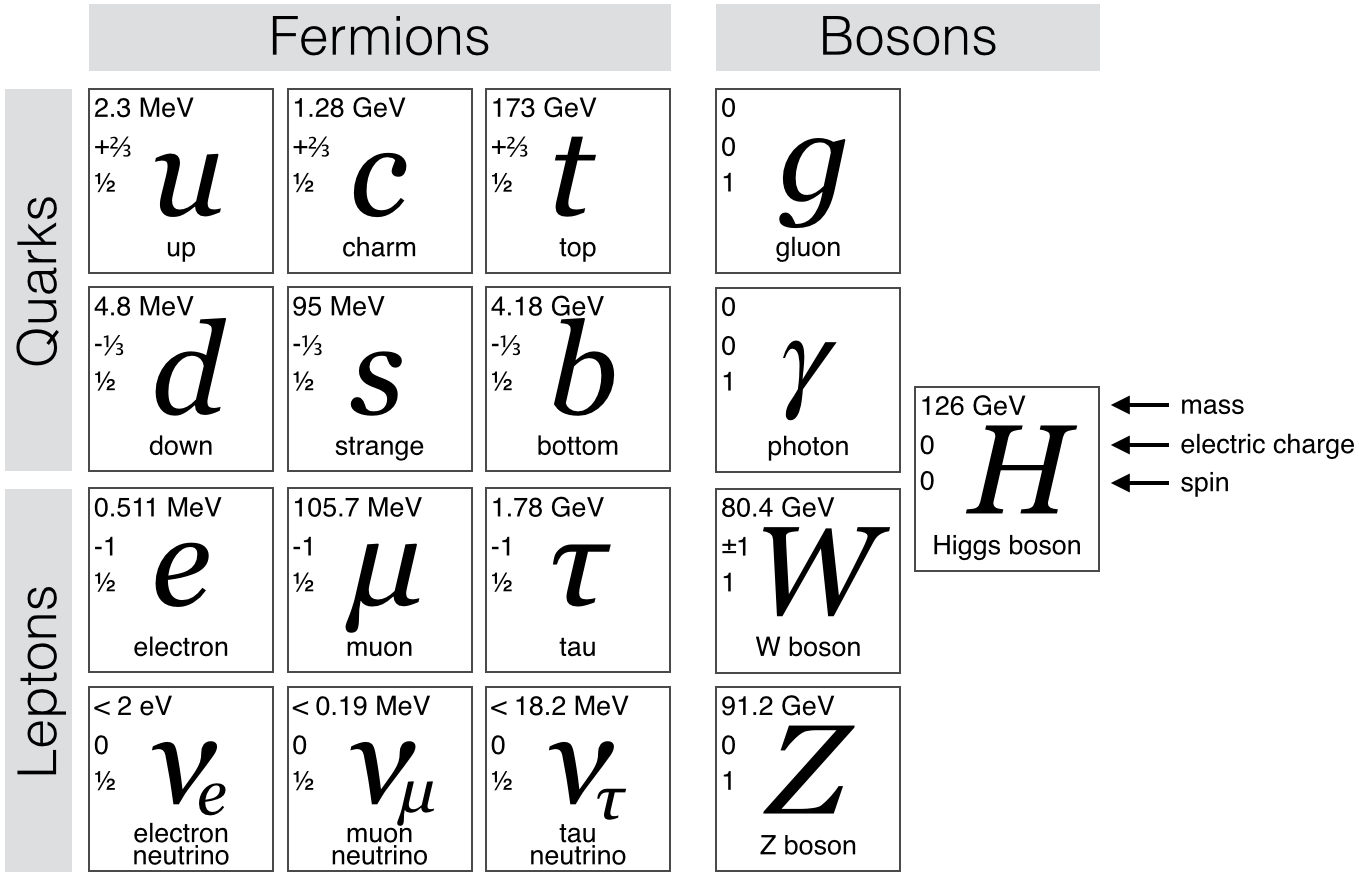
\includegraphics[width=\largefigwidth]{tex/motivation/sm_particles}
	\caption{The particle content of the \ac{SM}. Particle masses from \cite{PDG}.
	\todo[inline]{Should I remove the Higgs mass here?}}
	\label{fig:sm_particles}
\end{figure}

The elementary particles of the \ac{SM} are summarised in \Figure~\ref{fig:sm_particles}.
They are naturally separated into bosons (integer spin) and fermions (half-integer spin).
In addition to the gauge bosons previously introduced, the Higgs boson is a by-product
of electroweak symmetry breaking (described in \Section~\ref{sec:ewsb}) and its
couplings are proportional to mass. The twelve flavours of fermions are categorised 
according to the interactions they experience, or equivalently the charges they posses: 
quarks (strong, electromagnetic, weak), charged leptons (electromagnetic, weak) and 
neutrinos (weak). The fermions are also arranged in three generations of increasing
mass - the first generation are stable since they cannot decay to lower mass particles.
Most particles have an associated antiparticle with identical mass but inverted internal 
quantum numbers.

    \section{Electroweak unification}
      \label{sec:ewsb}
      %!TEX root = ../../thesis.tex

The first theory of weak interactions was a four-point interaction with Fermi coupling 
constant \unit{$G_{\text{F}} = 1.166\times 10^{-5}$}{\GeV\rpsquared}. Although successful 
in describing low energy phenomena, such as nuclear $\beta$-decay and muon decay, at 
energies above \unit{\about300}{\GeV} the theory predicted cross sections which violate 
unitarity \cite{Aitchison}.

The solution was to introduce charged vector bosons (\PWpm bosons) to mediate the weak 
interaction, similar to the exchange of photons in \ac{QED}. However, unlike \ac{QED}, 
the weak interaction is short ranged and therefore its exchange bosons must be massive. 
Since the propagator for a particle of mass $m$ and momentum $p$ contains a factor 
$1 / (p^2 - m^2)$, in the low energy limit we can relate to Fermi's theory and identify
\begin{equation}
	G_{\text{F}} \sim g^2 / m_{\PW}^2
\end{equation}
where $g$ is the coupling of the vector boson. Thus, at low energies, the strength of the 
weak interaction is suppressed by the mass of the exchange boson.

At this time, there were two key obstacles to unifying the electromagnetic and weak 
interactions. First, the discovery of parity violation in cobalt-60 $\beta$-decay 
implied the weak interaction has a \VminusA structure, whereas \ac{QED} has a pure V 
structure \cite{Wu:1957}.\footnote{
	Five bilinear covariants can be constructed from the Dirac $\gamma$ matrices, which 
	are named according to how they transform under parity: scalar, pseudoscalar, vector, 
	axial vector and tensor.
}
Second, the \PWpm bosons are massive whilst photons are massless. This was a major 
problem because gauge bosons are inherently massless.\footnote{
	Consider the gauge transformation of a Yang-Mills gauge field 
	$\bvec{W}_{\mu} \rightarrow \bvec{W}_{\mu} - \partial_{\mu} \bvec{\alpha}(x)
	- g \lbrack \bvec{\alpha}(x) \times \bvec{W}_{\mu} \rbrack$. Clearly the mass term 
	$-\tfrac{1}{2}m^2 \bvec{W}_{\mu} \cdot \bvec{W}^{\mu}$ is not gauge invariant, and 
	hence the gauge boson is massless.}
In fact, fermion masses were also forbidden by the chiral nature of the weak interaction, 
but were known to exist.\footnote{
	Consider a spinor as the sum of its left- and right-handed chiral states 
	$\psi = \psi_{\text{L}} + \psi_{\text{R}}$. Then the Dirac mass term is 
	$-m \bar{\psi} \psi = -m (\bar{\psi}_{\text{R}} \psi_{\text{L}} + 
	\bar{\psi}_{\text{L}} \psi_{\text{R}})$. For a chiral theory, $\psi_{\text{L}}$ and
	$\psi_{\text{R}}$ behave differently under gauge transformations and thus the mass 
	term is not gauge invariant.
}

Glashow's proposal of an \EWgroup group was a major step forward \cite{Glashow:1961}. 
This model describes three gauge fields \rowthreevec{W^1_{\mu}}{W^2_{\mu}}{W^3_{\mu}} 
which couple to weak isospin $T$ with strength $g$, and a single gauge field $B_{\mu}$ 
which couples to weak hypercharge $Y$ with strength $g'$. The subscript L indicates 
that only left-handed chiral particles couple to the $W^i_{\mu}$ fields, explaining the 
\VminusA nature of the weak interaction whilst preserving \ac{QED}. The physical gauge 
fields are obtained through the mixing of these fields
\begin{align}
	W^{\pm}_{\mu} &= (W^1_{\mu} \mp i W^2_{\mu}) / \sqrt{2} \label{eq:Wfield} \\
	Z_{\mu} &= \cos\thetaW W^3_{\mu} - \sin\thetaW B_{\mu} \label{eq:Zfield} \\
	A_{\mu} &= \sin\thetaW W^3_{\mu} + \cos\thetaW B_{\mu} \label{eq:Afield}
\end{align}
where
\begin{equation}
	\cos\thetaW = g/\sqrt{g^2 + g'^2}
	\quad\quad \text{and} \quad\quad
	\sin\thetaW = g'/\sqrt{g^2 + g'^2} \,. 
	\label{eq:weak_mixing}
\end{equation}
We identify $W^{\pm}_{\mu}$ with the \PWpm bosons, $A_{\mu}$ with the photon 
and $Z_{\mu}$ with a new neutral \PZ boson. Weak neutral currents were later confirmed 
experimentally \cite{Gargamelle:1973}. 

Glashow's \EWgroup theory therefore predicts the interaction of fermions, in left-handed 
\SUgroup{2} doublets and right-handed \SUgroup{2} singlets (see 
\Table~\ref{tab:ew_fermions}), with \PWpm, \PZ and \Pphoton 
exchange bosons. Gauge boson self-interactions are also expected due to the non-abelian 
nature of the \ac{EW} theory. The \PWpm bosons couple to weak isospin $T$ with strength 
$g$, the \PZ boson couples vectorially to $c_{\text{V}}$ and axially to $c_{\text{A}}$ 
with strength $g/(2\cos\thetaW)$, and the photon couples to electric charge $Q$ with 
strength $e = g\sin\thetaW$, where
\begin{align}
	c_{\text{V}} &= T_3 - 2 Q \sin^2\thetaW \,,\quad\quad c_{\text{A}} = T_3 \\
	Q   &= T_3 + \frac{Y}{2} \,.
\end{align}

\begin{table}[b]
	\begin{tabular}{ccc@{\hskip 1cm}cccc}
		\toprule
		& & & $T$ & $T_3$ & $Y$ & $Q$ \\
		\midrule
		\multirow{2}{*}{$\colvector{\Pnue\\ \Pe}_{\!\!\!\text{L}}$} & 
		\multirow{2}{*}{$\colvector{\Pnum\\ \Pmu}_{\!\!\!\text{L}}$} & 
		\multirow{2}{*}{$\colvector{\Pnut\\ \Ptau}_{\!\!\!\text{L}}$} & 
		$\tfrac{1}{2}$ & $+\tfrac{1}{2}$ & $-1$ & 0 \\
		& & & $\tfrac{1}{2}$ & $-\tfrac{1}{2}$ & $-1$ & $-1$ \\
		$\Pnue_{\text{R}}$ & $\Pnum_{\text{R}}$ & $\Pnut_{\text{R}}$ & 0 & 0 & 0 & 0 \\
		$\Pe_{\text{R}}$ & $\Pmu_{\text{R}}$ & $\Ptau_{\text{R}}$ & 0 & 0 & $-2$ & $-1$ \\
		\midrule
		\multirow{2}{*}{$\colvector{\Pup\\ \Pdown'}_{\!\!\!\text{L}}$} & 
		\multirow{2}{*}{$\colvector{\Pcharm\\ \Pstrange'}_{\!\!\!\text{L}}$} & 
		\multirow{2}{*}{$\colvector{\Ptop\\ \Pbottom'}_{\!\!\!\text{L}}$} & 
		$\tfrac{1}{2}$ & $+\tfrac{1}{2}$ & $+\tfrac{1}{3}$ & $+\tfrac{2}{3}$ \\
		& & & $\tfrac{1}{2}$ & $-\tfrac{1}{2}$ & $+\tfrac{1}{3}$ & $-\tfrac{1}{3}$ \\
		$\Pup_{\text{R}}$ & $\Pcharm_{\text{R}}$ & $\Ptop_{\text{R}}$ & 0 & 0 & $+\tfrac{4}{3}$ & $+\tfrac{2}{3}$ \\
		$\Pdown_{\text{R}}$ & $\Pstrange_{\text{R}}$ & $\Pbottom_{\text{R}}$ & 0 & 0 & $-\tfrac{2}{3}$ & $-\tfrac{1}{3}$ \\
		\bottomrule
	\end{tabular}
	\caption{The weak isospin $T$, weak hypercharge $Y$ and electric charge $Q$ of the 
	fermions. In charged currents, the states that couple to \Pup-type 
	quarks are superpositions of \Pdown-type quarks and are denoted with a prime. 
	Although right-handed neutrinos are decoupled, recent observations of neutrino 
	oscillations suggest these might exist.}
	\label{tab:ew_fermions}
\end{table}

Unfortunately, it was necessary to explicitly break the symmetry by adding mass terms for 
the \PWpm and \PZ bosons by hand. Initial attempts to invoke a mechanism of \ac{SSB} were 
hindered by the Goldstone theorem.



\subsection{The Goldstone theorem}
\label{sec:ewsb:goldstone}
\ac{SSB} arises when the vacuum state does not respect the symmetry in question. This can 
occur when a field acquires a non-zero vacuum expectation value. To see this, consider a 
complex scalar field $\phi$ described by the Lagrangian
\begin{equation}
	\mathcal{L} 
	= \parenths{\partial_{\mu}\phi^{\dagger}} \parenths{\partial^{\mu}\phi} 
	+ \mu^2 \phi^{\dagger}\phi - \lambda \parenths{\phi^{\dagger}\phi}^2
	\label{eq:lagr:goldstone}
\end{equation}
with positive $\mu^2$ and $\lambda$, giving a sombrero potential 
(\Figure~\ref{fig:sombrero}). 
Although $\mathcal{L}$ is invariant under global \Ugroup{1} transformations 
$\phi \rightarrow \eexp{-i\alpha} \phi$, there are infinite degenerate vacua
$\phi = \mu\eexp{-i\theta}/\sqrt{2\lambda}$ that are not invariant. In order to interact 
with the system, a single vacuum must be arbitrarily chosen, spontaneously breaking the 
\Ugroup{1} symmetry.

\begin{figure}[b]
	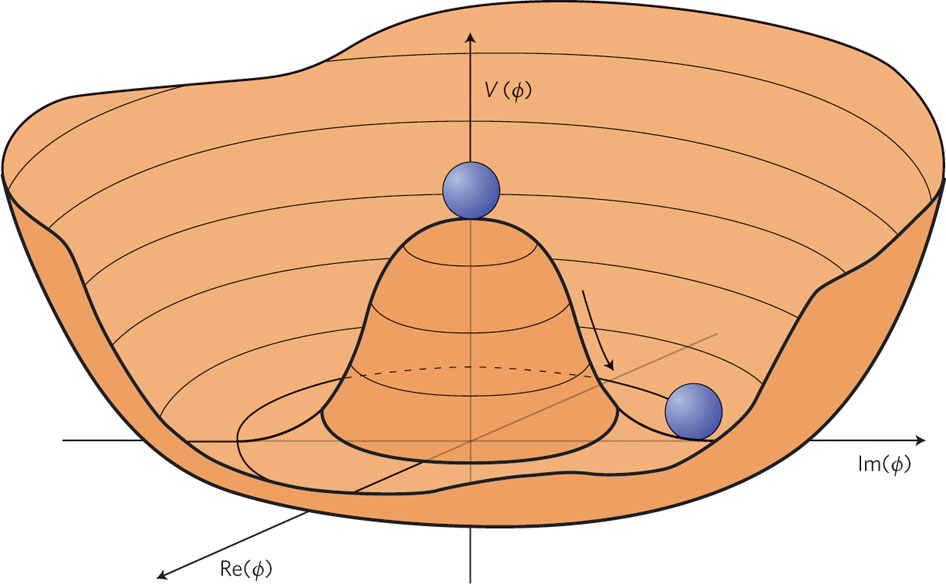
\includegraphics[width=\mediumfigwidth]{tex/motivation/sombrero}
	\caption{The sombrero potential, in which a vacuum state must be arbitrarily chosen, 
	spontaneously breaking the symmetry of the underlying Lagrangian.
	Fluctuations in the azimuthal direction correspond to a massless Nambu-Goldstone 
	boson. Fluctuations in the radial direction correspond to a massive Higgs boson.}
	\label{fig:sombrero}
\end{figure}

The Goldstone theorem states that \ac{SSB} of a continuous global symmetry will lead to 
the existence of a number of massless scalar Nambu-Goldstone bosons \cite{Goldstone:1962}.
This can be seen by considering radial and azimuthal excitations, $h\parenths{x}$ and 
$\theta\parenths{x}$, about the vacuum 
\begin{equation}
	\phi\parenths{x} = \frac{1}{\sqrt{2}} \sqbracs{v + h\parenths{x}} \eexp{-i\theta\parenths{x} / v}
\end{equation}
where $v = \mu/\sqrt{\lambda}$. When substituted into (\ref{eq:lagr:goldstone}), we get
\begin{equation}
	\mathcal{L} = \tfrac{1}{2}\partial_{\mu}\theta \partial^{\mu}\theta
	+ \tfrac{1}{2}\partial_{\mu}h \partial^{\mu}h
	- \mu^2 h^2
	+ \dots
\end{equation}
where the dots denote terms neither kinetic nor mass. 
We identify a massless Nambu-Goldstone boson (the $\theta$-mode) and a Higgs boson of 
mass $\sqrt{2}\mu$ (the $h$-mode).

In order to explain massive \PWpm and \PZ bosons, the electroweak symmetry must be broken.
But the Goldstone theorem suggested that this would predict massless scalar bosons, which
were not experimentally observed.



\subsection{The Higgs mechanism}
\label{sec:ewsb:higgs}
However, when \ac{SSB} of a continuous \textit{local} symmetry is studied, something 
remarkable happens. The Nambu-Goldstone bosons of the theory are `eaten' by the gauge 
bosons, giving them mass. The associated degrees of freedom appear as longitudinal 
components of the massive gauge bosons. This is known as the Higgs mechanism 
\cite{Englert:1964,Higgs:1964a,Higgs:1964b,Guralnik:1964,Higgs:1966}.

Consider the Lagrangian for a \Ugroup{1} gauge theory with a sombrero potential
\begin{equation}
	\mathcal{L} 
	= \parenths{D_{\mu}\phi}^{\dagger} \parenths{D^{\mu}\phi}
	- \tfrac{1}{4} F_{\mu\nu} F^{\mu\nu}
	+ \mu^2 \phi^{\dagger} \phi - \lambda \parenths{\phi^{\dagger} \phi}^2
	\label{eq:lagr:abelHiggs}
\end{equation}
where $D_{\mu} = \partial_{\mu} + iqA_{\mu}$ is the covariant derivative and $F_{\mu\nu} 
= \partial_{\mu}A_{\nu} - \partial_{\nu}A_{\mu}$ is the field tensor. This is invariant 
under local \Ugroup{1} transformations $\phi \rightarrow \eexp{-i\alpha\parenths{x}} \phi$
when accompanied by a gauge transformation of the potential 
$A_{\mu} \rightarrow A_{\mu} + \tfrac{1}{q}\partial_{\mu} \alpha\parenths{x}$.

We are free to choose the unitary gauge $\alpha\parenths{x} = -\theta\parenths{x}/v$,
absorbing the $\theta$-mode into the photon field 
$A_{\mu} \rightarrow A_{\mu} - \tfrac{1}{qv}\partial_{\mu} \theta\parenths{x}$. 
Ultimately, the final result is gauge-independent, but other choices require the 
Nambu-Goldstone bosons to be explicitly included in the Feynman rules. Since the 
$\theta$-mode is `gauged away', excitations about the vacuum become
\begin{equation}
	\phi\parenths{x} = \frac{1}{\sqrt{2}} \sqbracs{v + h\parenths{x}}
\end{equation}
and the Lagrangian (\ref{eq:lagr:abelHiggs}) becomes
\begin{equation}
	\mathcal{L}
	= \tfrac{1}{2} q^2 v^2 A_{\mu} A^{\mu}
	- \tfrac{1}{4} F_{\mu\nu}F^{\mu\nu}
	+ \tfrac{1}{2} \partial_{\mu}h \partial^{\mu}h
	- \mu^2 h^2
	+ \dots
\end{equation}
where the dots denote terms neither kinetic nor mass. 
The Nambu-Goldstone boson is no longer present and the photon has acquired a mass $qv$.
Again, there is a massive scalar Higgs boson as a by-product of the \ac{SSB}.



\subsection{Glashow-Salam-Weinberg electroweak theory}
The Higgs mechanism can be extended to non-abelian gauge theories, as was necessary to 
describe electroweak symmetry breaking \cite{Kibble:1967,Weinberg:1967,Salam:1968}.
Consider the Lagrangian for an \SUgroup{2}\cross\Ugroup{1} gauge theory with a sombrero
potential
\begin{equation}
	\mathcal{L} 
	= \parenths{D_{\mu}\phi}^{\dagger} \parenths{D^{\mu}\phi}
	- \tfrac{1}{4} \bvec{F}_{\mu\nu} \cdot \bvec{F}^{\mu\nu}
	- \tfrac{1}{4} G_{\mu\nu} G^{\mu\nu}
	+ \mu^2 \phi^{\dagger} \phi - \lambda \parenths{\phi^{\dagger} \phi}^2
	\label{eq:lagr:ewHiggs}
\end{equation}
where $D_{\mu} = \partial_{\mu} + \tfrac{i}{2} g \bvec{\tau} \cdot \bvec{W}_{\mu} + 
\tfrac{i}{2} g' Y B_{\mu}$ is the covariant derivative, and $\bvec{F}_{\mu\nu} = 
\partial_{\mu}\bvec{W}_{\nu} - \partial_{\nu}\bvec{W}_{\mu} - g \bvec{W}_{\mu} \cross 
\bvec{W}_{\nu}$ and $G_{\mu\nu} = \partial_{\mu}B_{\nu} - \partial_{\nu}B_{\mu}$ are the
field tensors. In this case, $\phi$ is an \SUgroup{2} doublet of complex scalar fields
\begin{equation}
	\phi = \colvector{\phi^+\\\phi^0} = \frac{1}{\sqrt{2}} \colvector{ \phi_1 + i\phi_2\\ \phi_3 + i\phi_4}.
\end{equation}

Again, there are infinite degenerate vacua satisfying 
$\parenths{\phi_1^2 + \phi_2^2 + \phi_3^2 + \phi_4^2} = \mu^2/\lambda$. In analogue with 
the abelian Higgs mechanism, the unitary gauge absorbs the $\phi_1$, $\phi_2$ and 
$\phi_4$-modes into the gauge fields. Thus, considering excitations about the vacuum
\begin{equation}
	\phi\parenths{x} = \frac{1}{\sqrt{2}} \colvector{0\\  
	v + h\parenths{x}} \label{eq:higgs_doublet}
\end{equation}
the Lagrangian (\ref{eq:lagr:ewHiggs}) becomes
\begin{align}
	\mathcal{L} &= \tfrac{1}{8} g^2 v^2 \bvec{W}_{\mu} \cdot \bvec{W}^{\mu} - \tfrac{1}{4} \bvec{F}_{\mu\nu} \cdot \bvec{F}^{\mu\nu} + \tfrac{1}{8} v^2 g'^2 B_{\mu} B^{\mu} - \tfrac{1}{4} v^2 gg' B_{\mu} W_{3}^{\mu} - \tfrac{1}{4} G_{\mu\nu} G^{\mu\nu} \nonumber \\
	&\quad\quad {} + \tfrac{1}{2} \partial_{\mu}h \partial^{\mu}h - \mu^2 h^2 + \dots \\
	&= \tfrac{1}{4} g^2 v^2 W^{+}_{\mu} W^{-\mu} - \tfrac{1}{2} \parenths{\partial_{\mu}W^{+}_{\nu} - \partial_{\nu}W^{+}_{\mu}} \parenths{\partial^{\mu}W^{-\nu} - \partial^{\nu}W^{-\mu}} \nonumber \\
	&\quad\quad {} + \tfrac{1}{8} v^2 \parenths{g^2 + g'^2} Z_{\mu} Z^{\mu} - \tfrac{1}{4} \parenths{\partial_{\mu}Z_{\nu} - \partial_{\nu}Z_{\mu}} \parenths{\partial^{\mu}Z^{\nu} - \partial^{\nu}Z^{\mu}} - \tfrac{1}{4} F_{\mu\nu} F^{\mu\nu} \nonumber \\
	&\quad\quad {} + \tfrac{1}{2} \partial_{\mu}h \partial^{\mu}h - \mu^2 h^2 + \dots
\end{align}
where the dots denote terms neither kinetic nor mass, $F_{\mu\nu}$ is the field tensor of
\ac{QED}, and the expression has been rewritten in terms of the physical gauge fields 
using (\ref{eq:Wfield}), (\ref{eq:Zfield}) and (\ref{eq:Afield}). The \PWpm bosons 
acquire a mass $gv/2$ and the \PZ boson acquires a mass $v \sqrt{\parenths{g^2+g'^2}}/2$, 
while the photon is massless. Again, all Nambu-Goldstone bosons are gone and a Higgs 
boson has appeared as a by-product of the \ac{SSB}.

This theory predicts a striking relation between the gauge boson masses, using 
(\ref{eq:weak_mixing})
\begin{equation}
	\mW = \mZ \cos\thetaW
\end{equation}
which was experimentally verified once the \PW and \PZ bosons were discovered 
\cite{UA1:Wboson,UA2:Wboson,UA1:Zboson,UA2:Zboson,UA1:1989}. It also predicted a massive 
scalar Higgs boson, whose mass could not be determined from the other parameters of the 
theory.

Fermion masses can also be incorporated into \ac{EW} theory through Yukawa couplings.
Consider a coupling between the electron-type \SUgroup{2} doublet (see 
\Table~\ref{tab:ew_fermions}), the Higgs doublet $\phi$ given in 
(\ref{eq:higgs_doublet}), and the electron \SUgroup{2} singlet
\begin{align}
	\mathcal{L}_{\Pe}^{\text{Yuk}} &= -g_{\Pe} \parenths{\overline{\Plepton}_{\Pe \text{L}} \phi \Pe_{\text{R}} + \overline{\Pe}_{\text{R}} \phi^{\dagger} \Plepton_{\Pe \text{L}}} \\
	&= -\frac{g_{\Pe}}{\sqrt{2}} \sqbracs{v + h} \parenths{\overline{\Pe}_{\text{L}} \Pe_{\text{R}} + \overline{\Pe}_{\text{R}} \Pe_{\text{L}}}
\end{align}
where $g_e$ is the electron Yukawa coupling. The electron has acquired a mass 
$g_{\Pe}v/\sqrt{2}$ and the coupling of the Higgs boson to the electron is proportional 
to that mass (specifically $m_e/v$).

Finally, we note a similar phenomenon in superconductors. There, the \Ugroup{1} symmetry 
of \ac{QED} is spontaneously broken, as in \Section~\ref{sec:ewsb:higgs}, giving mass to 
the photon and thereby producing the Meissner effect. In fact, Higgs bosons have been 
observed in the Raman spectra of superconductors \cite{Superconductivity}. However, a 
major difference is that the bosonic field is a Bose-Einstein condensate of loosely bound 
electron pairs (known as Cooper pairs), and therefore the \ac{SSB} is dynamic. This is 
only possible due to lattice vibrations of the underlying solid. It is natural to ask 
whether a similar dynamic mechanism could be used to break \ac{EW} symmetry, where the 
Higgs boson is a composite particle. This is an active area of research, though will not 
be explored here.

    \section{Properties of the Higgs boson}
      \label{sec:properties}
      %!TEX root = ../../thesis.tex

The Higgs boson is predicted to have zero spin and positive parity, whilst being 
electrically neutral and colourless. It couples directly to massive particles. Other 
properties, such as production cross sections and branching ratios (BRs) of decay, must be 
calculated as a function of its mass, which is not predicted by the SM.

% Experimental signatures for the Higgs boson are categorised according to production 
% mode and decay channel.

At a hadron collider such as the LHC, the important production modes are gluon-gluon 
fusion (ggF), vector boson fusion (VBF), Higgs-strahlung (\WH and \ZH) and top fusion 
(\ttH). Example Feynman diagrams are shown in \Figure~\ref{fig:feyn}. We note that the 
Higgs boson does not couple to massless gluons, therefore ggF proceeds via loops of 
massive coloured particles (predominantly the top quark due to its large mass). 

\begin{figure}[b]
	\null\hfill
	\begin{subfigure}[b]{0.4\textwidth}
		\centering
		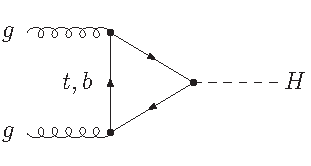
\includegraphics[width=\textwidth]{axodraw/ggF.pdf}
		\caption{Gluon-gluon fusion (ggF)}
		\label{fig:feyn:ggF}
	\end{subfigure}
	\hfill
	\begin{subfigure}[b]{0.4\textwidth}
		\centering
		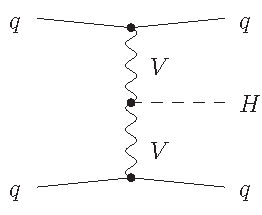
\includegraphics[width=0.75\textwidth]{axodraw/VBF.pdf}
		\caption{Vector boson fusion (VBF)}
		\label{fig:feyn:VBF}
	\end{subfigure}
	\hfill\null
	\\\bigskip
	\null\hfill
	\begin{subfigure}[b]{0.4\textwidth}
		\centering
		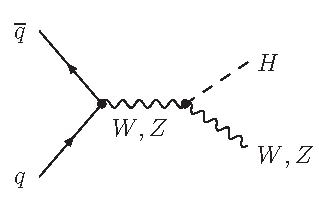
\includegraphics[width=0.8\textwidth]{axodraw/VH.pdf}
		\caption{Higgs-strahlung (\WH and \ZH)}
		\label{fig:feyn:VH}
	\end{subfigure}
	\hfill
	\begin{subfigure}[b]{0.4\textwidth}
		\centering
		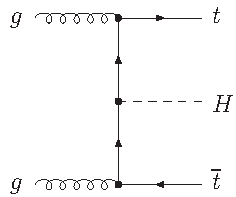
\includegraphics[width=0.625\textwidth]{axodraw/ttH.pdf}
		\caption{Top fusion (\ttH)}
		\label{fig:feyn:ttH}
	\end{subfigure}
	\hfill\null
	\caption{Examples of tree-level Feynman diagrams for the Higgs production processes relevant at the LHC.}
	\label{fig:feyn}
\end{figure}

The production cross sections at the LHC are shown in \Figure~\ref{fig:higgs_xs}. 
Whilst ggF clearly dominates these rare processes, it suffers from large 
experimental backgrounds. The four other modes feature additional final state particles 
which can aid identification. For example, VBF has two well-separated quarks with no 
colour exchange between them.

\begin{figure}
	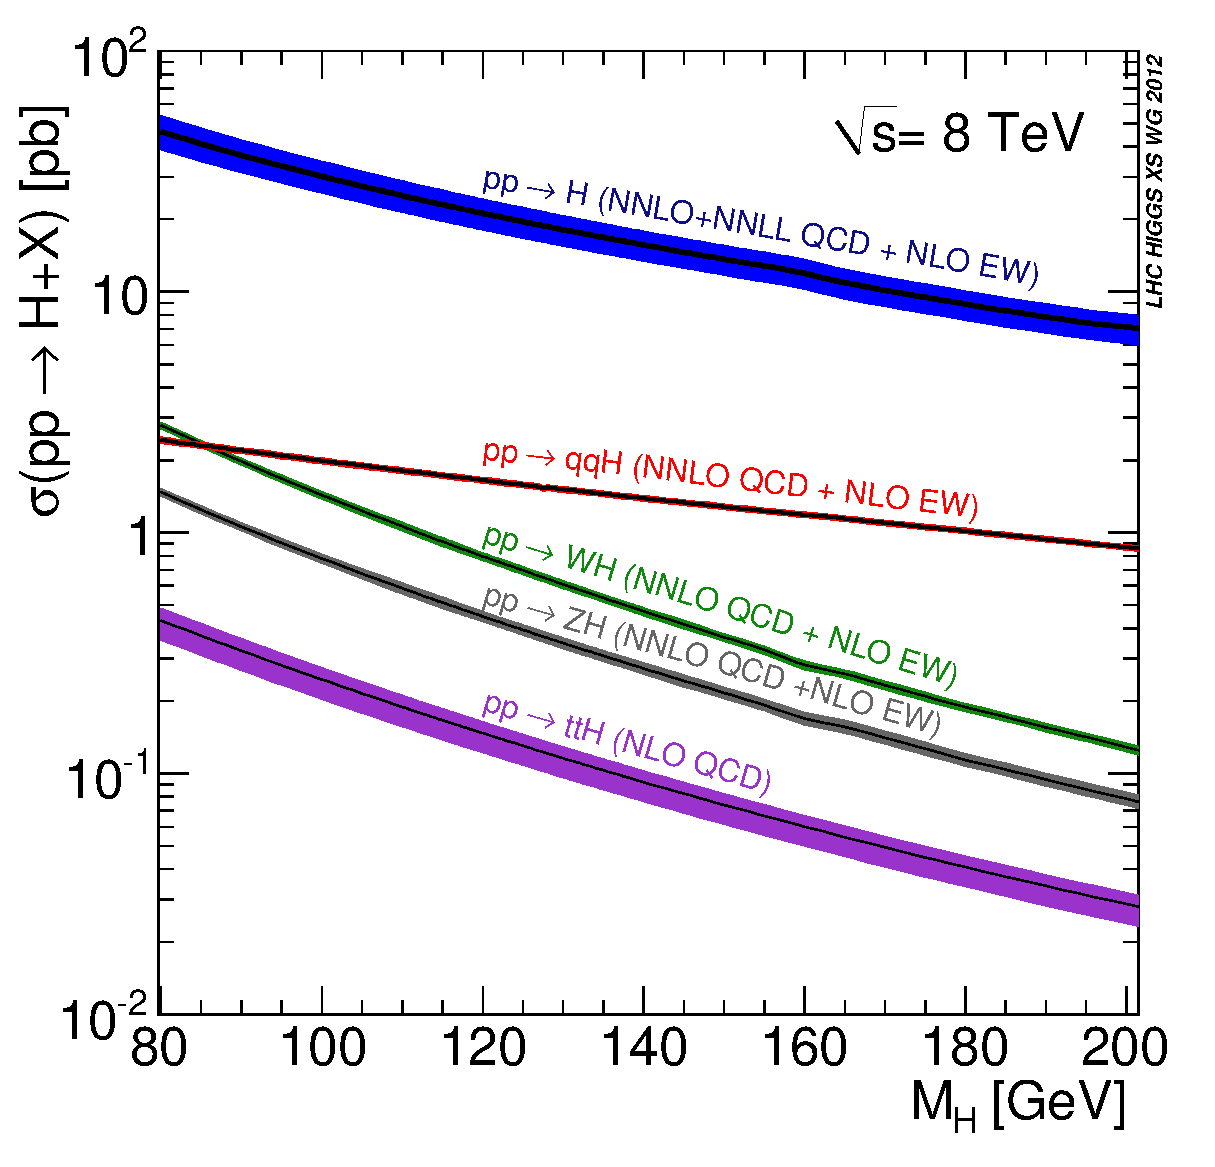
\includegraphics[width=0.48\textwidth]{tex/motivation/xs_lowrange}
	\hfill
	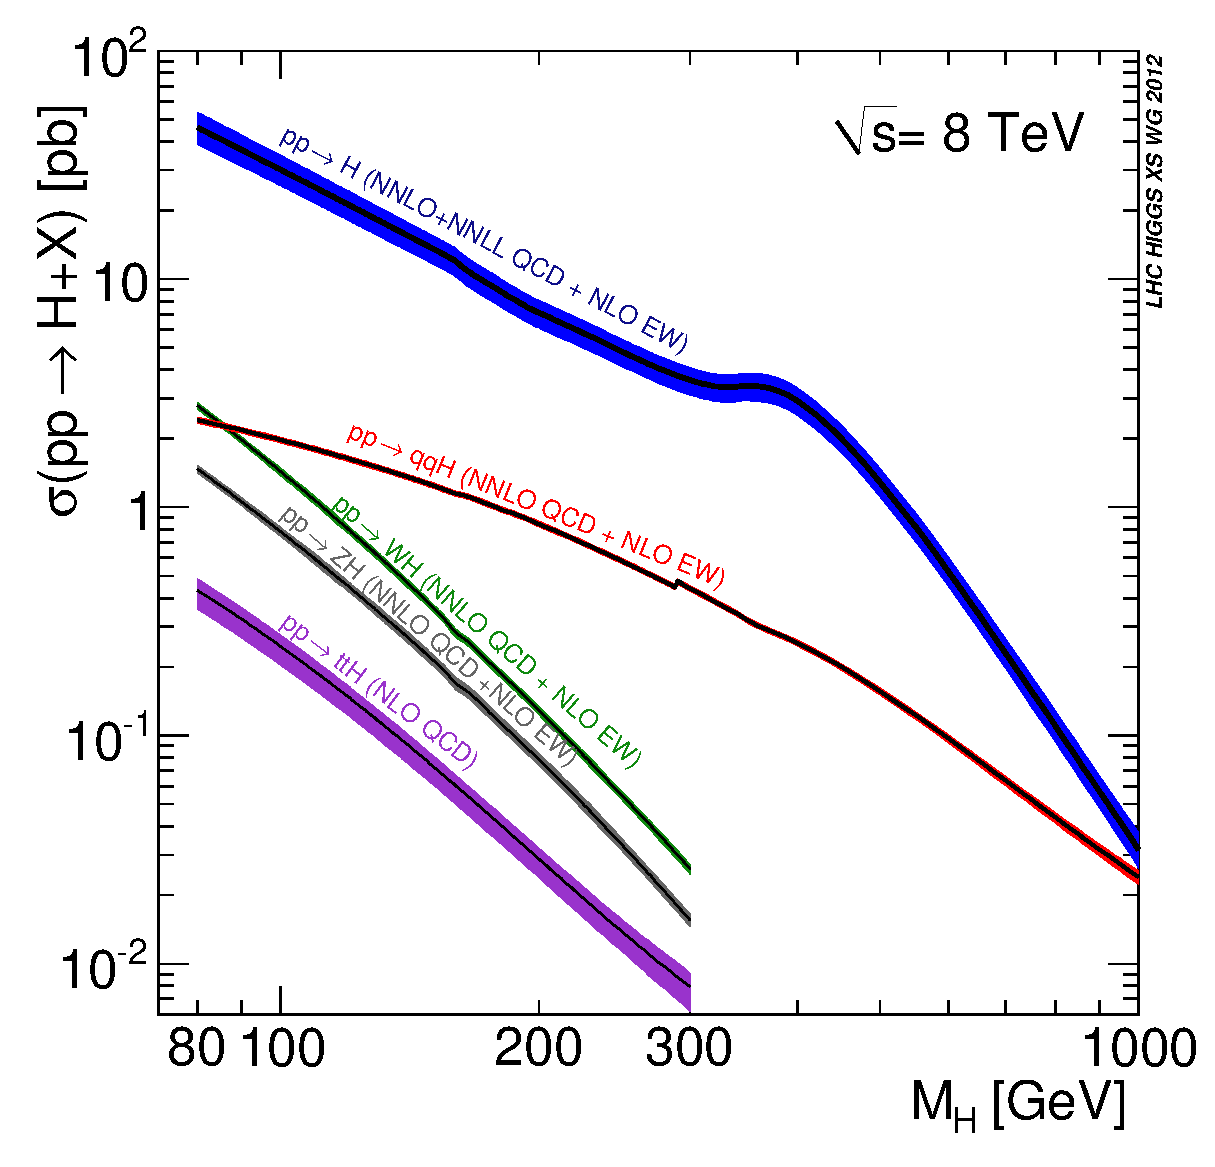
\includegraphics[width=0.48\textwidth]{tex/motivation/xs_fullrange}
	\caption{Higgs boson production cross sections versus mass at 
	\unit{$\sqrt{s} = 8$}{\TeV} for a low mass range (left) and an expanded mass range 
	(right) \cite{YR2}. Theoretical uncertainties are shown as bands. The production modes
	are ggF (blue), VBF (red), \WH (green), \ZH (grey) and \ttH (purple).}
	\label{fig:higgs_xs}
\end{figure}

Since the lifetime of the Higgs boson is very short, it is never directly observed in a 
detector. Therefore it is important to understand the BRs of its decays 
(\Figure~\ref{fig:higgs_br}). Na\"{i}vely, these are understood from the Higgs boson coupling to mass and the kinematic requirement $m_{\PHiggs} > m_X + m_Y$ for a decay
\HepProcess{\PHiggs \HepTo XY}. This is complicated by off-shell particles (\eg a low mass
Higgs boson may decay to \HepProcess{\PW \PW^{*}}). 
Also, the \HepProcess{\Pphoton \Pphoton}, \HepProcess{\PZ \Pphoton} and 
\HepProcess{\Pgluon \Pgluon} decay modes are different since they feature massless 
particles, and therefore proceed via loops of massive charged particles (electric charge 
for \HepProcess{\Pphoton \Pphoton} and \HepProcess{\PZ \Pphoton}, colour charge for 
\HepProcess{\Pgluon \Pgluon}).

Designing a sensitive experimental search strategy for the Higgs boson can be difficult. 
In decay channels featuring weak bosons, the subsequent decay of the \PW or \PZ boson must 
also be considered. These are more likely to decay to quarks than to leptons, but the 
former suffers from large backgrounds at hadron colliders. Similarly, the 
\HepProcess{\Pbottom \APbottom} decay has the largest BR for low \mH but suffers from 
huge backgrounds. The sensitivity can be improved by combining with a more distinguished 
production mode, such as \WH or \ZH, but this reduces the production cross section.

\begin{figure}
	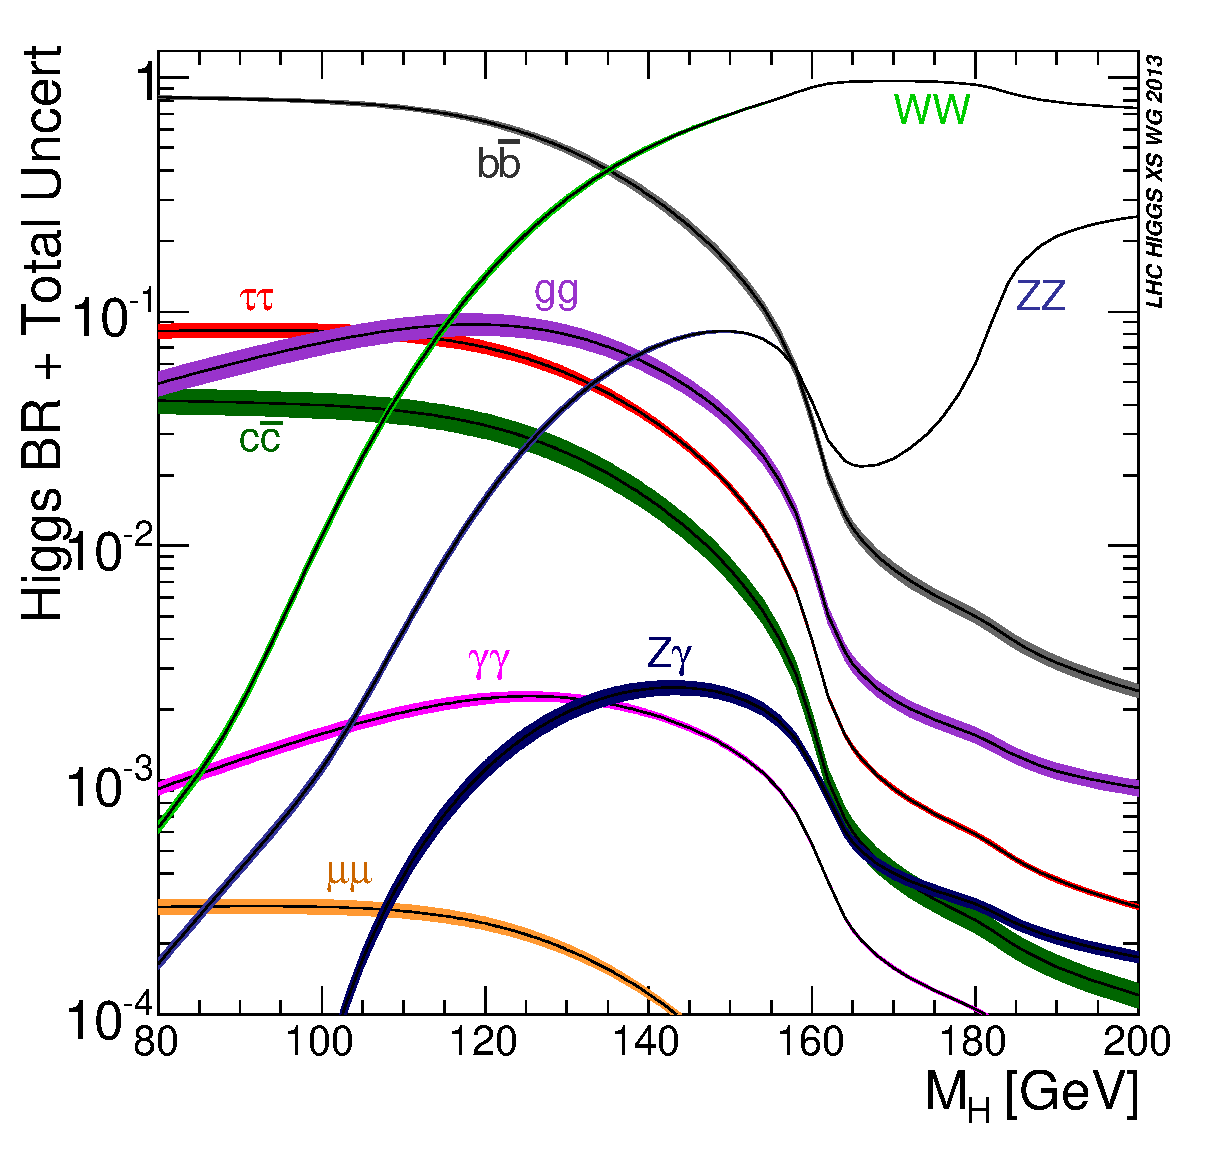
\includegraphics[width=0.48\textwidth]{tex/motivation/BR_lowrange}
	\hfill
	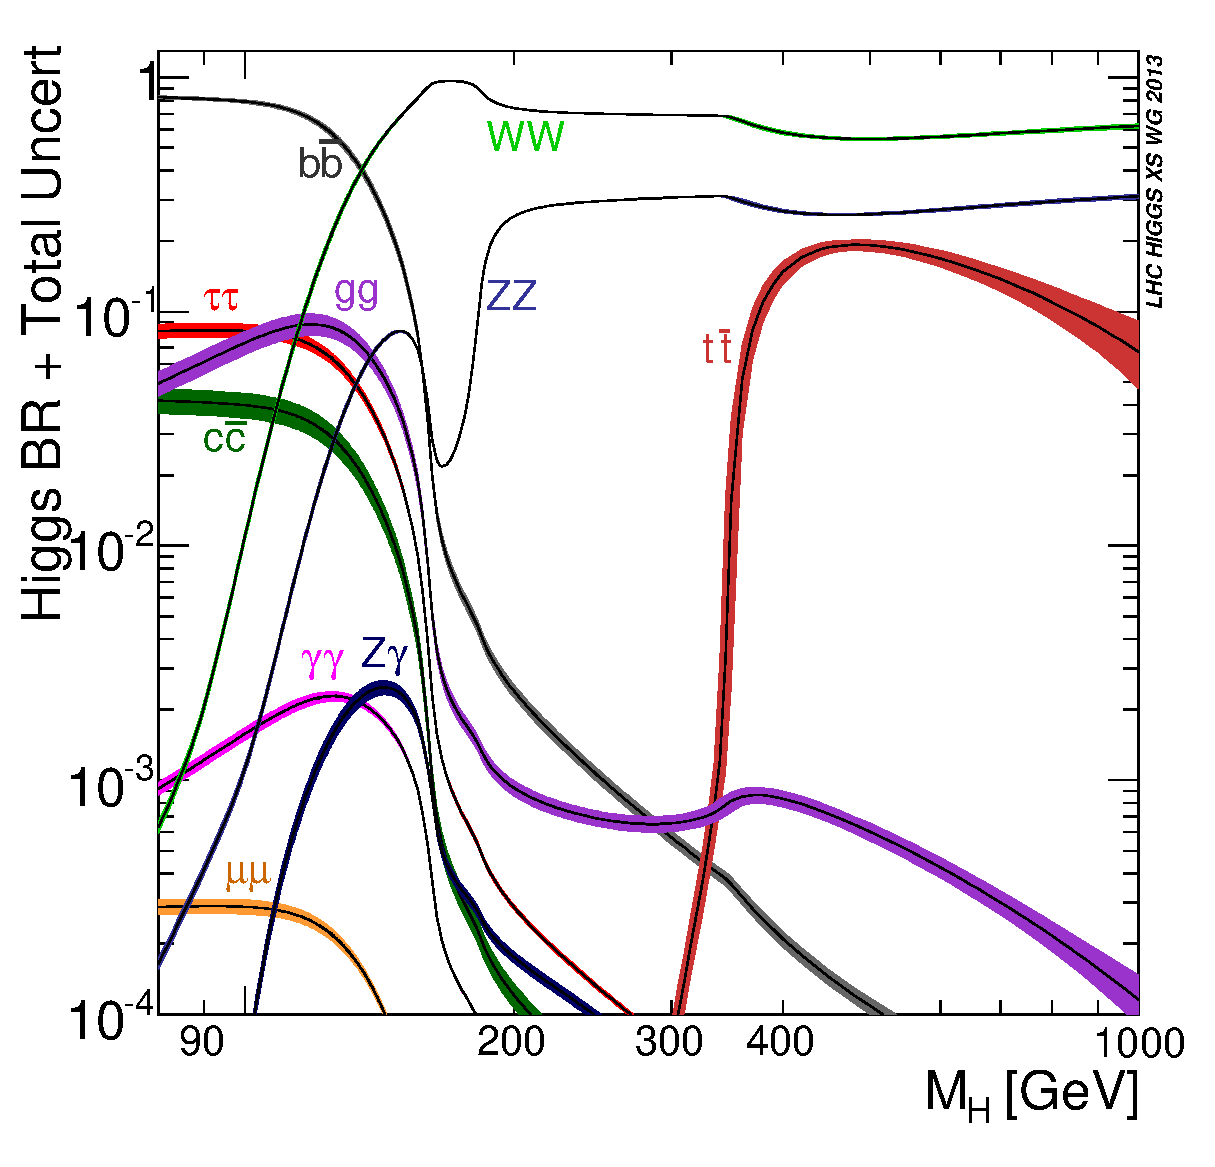
\includegraphics[width=0.48\textwidth]{tex/motivation/BR_fullrange}
	\caption{Branching ratios of Higgs boson decay versus mass for a low mass range (left) 
	and an expanded mass range (right) \cite{YR3}. Theoretical uncertainties are shown as 
	bands.}
	\label{fig:higgs_br}
\end{figure}

    \section{Pre-LHC constraints on the Higgs boson mass}
      \label{sec:prior_constraints}
      %!TEX root = ../../thesis.tex

Neglecting Yukawa interactions, the EW sector of the SM contains several free 
parameters that must be experimentally determined: two couplings ($g$, $g'$) and two 
Higgs sector parameters ($\mu$, $\lambda$). Using relations in \Section~\ref{sec:ewsb}, 
it is advantageous to choose an alternative set of independent parameters more closely 
connected to experiment: \alphaEM, \mW, \mZ, \mH. Finding the Higgs boson and 
measuring its mass is therefore of fundamental importance to understanding the EW 
sector, and this was a primary goal of the LHC physics program.

Prior to the LHC, the value of \mH was constrained through direct searches at 
previous colliders, global fits of other electroweak observables and theoretical 
considerations.



\subsection{Direct searches}
\label{sec:prior_constraints:direct}

Although masses below \unit{4}{\GeV} were excluded from \PB, \PUpsilon and \PK meson 
decays \cite{PDG:1988}, the first meaningful searches for a Higgs boson were 
performed at LEP (CERN, Geneva), which ran from 1989 to 2000. This was a circular 
\epluseminus collider with a centre-of-mass (CM) energy tuned to the \PZ-pole and then 
later varied between 189 and \unit{209}{\GeV}. A combined search for \ZH was performed 
using a total integrated luminosity of \unit{2.5}{\invfb}, which excluded 
\unit{$\mH < 114.4$}{\GeV} at the 95\% confidence level (CL) \cite{LEP:2003}.

Further searches were performed at the Tevatron (FNAL, Illinois), which ran from 1987
to 2011. This was a circular \ppbar collider with CM energies of \unit{1.8}{\TeV}
and \unit{1.96}{\TeV}. In 2010, searches using a variety of production and decay modes 
were combined across experiments using a total integrated luminosity of up to
\unit{12.6}{\invfb}. Masses below \unit{109}{\GeV} and between 158 and \unit{175}{\GeV} 
were excluded at the 95\% CL \cite{Tevatron:2010}.

% \begin{figure}
% 	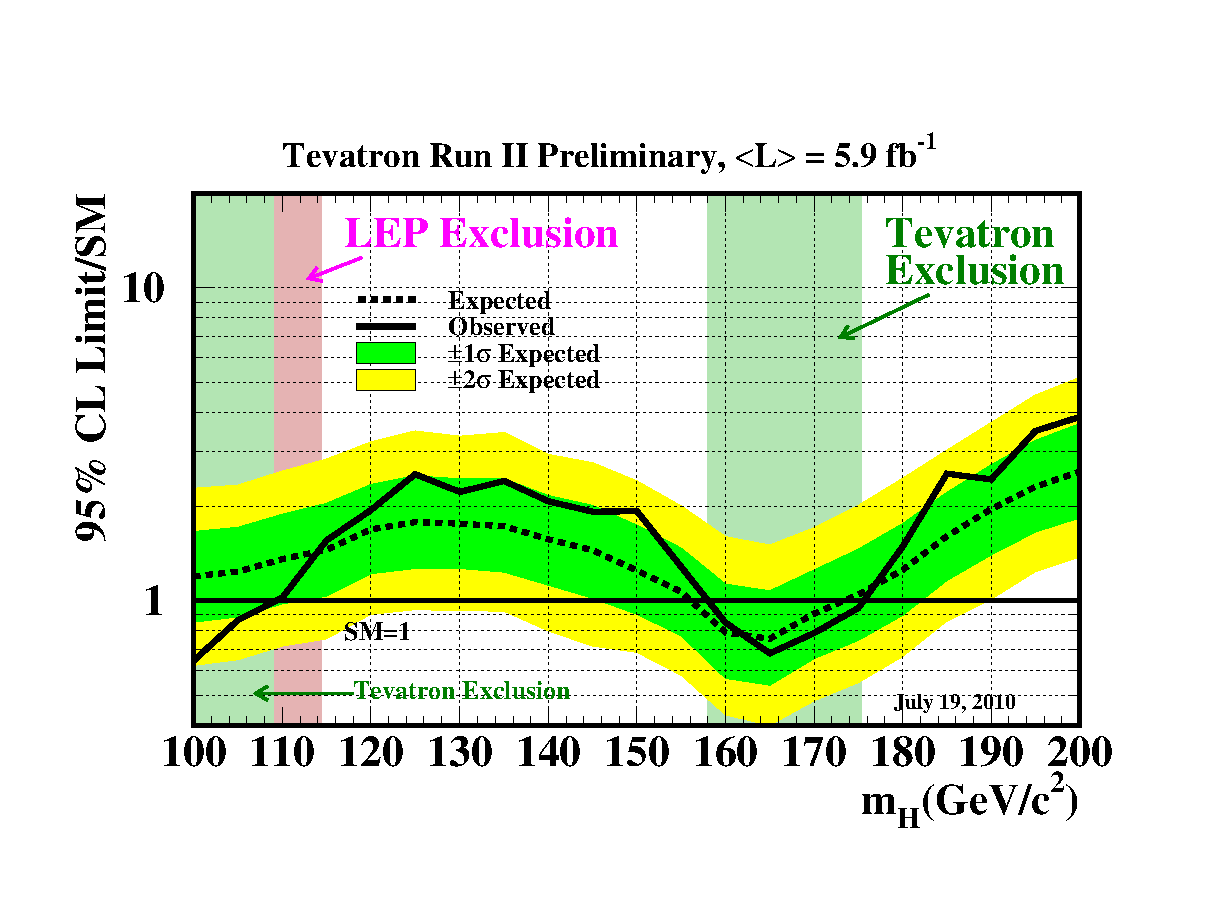
\includegraphics[width=\mediumfigwidth]{tex/motivation/tevatron_limit}
% 	\caption{Observed and expected 95\% \ac{CL} upper limits on the ratio to the \ac{SM} 
% 	cross section versus \mH, obtained through combination of multiple CDF and \dzero 
% 	analyses \cite{Tevatron:2010}. The analyses use datasets corresponding to integrated 
% 	luminosities up to \unit{5.9}{\invfb} at CDF and up to \unit{6.7}{\invfb} at \dzero.}
% 	\label{fig:existing_limits}
% \end{figure}



\subsection{Precision electroweak fits}
\label{sec:prior_constraints:ew_fits}

The SM predicts that many observables will depend upon \mH through loop corrections,
and it is therefore possible to infer \mH through precision EW measurements. Since 
the leading \mH dependence is logarithmic, the inferred constraints are weaker than those
used to predict the top mass (where the dependence is quadratic).

Performing a global fit of various electroweak measurements at the LEP, SLC and
Tevatron colliders (\eg \mW, \mZ, $m_{\Ptop}$), in July 2010 it was possible to exclude 
\mH $>$ \unit{158}{\GeV} at the 95\% CL \cite{Gfitter:2008}. However, the best fit 
value was excluded by direct searches, as shown in \Figure~\ref{fig:ewfit}.

\begin{figure}[t]
	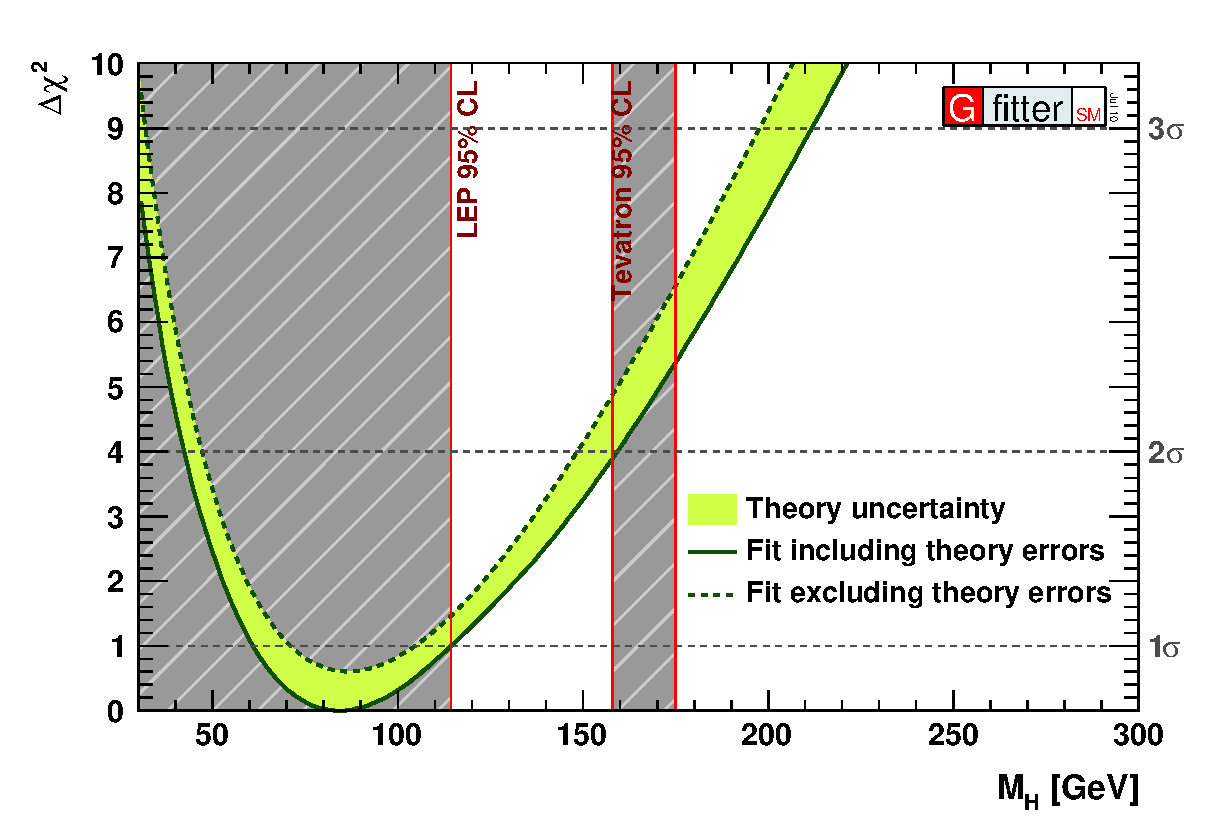
\includegraphics[width=0.495\textwidth]{tex/motivation/ewfit_nodirect}
	\hfill
	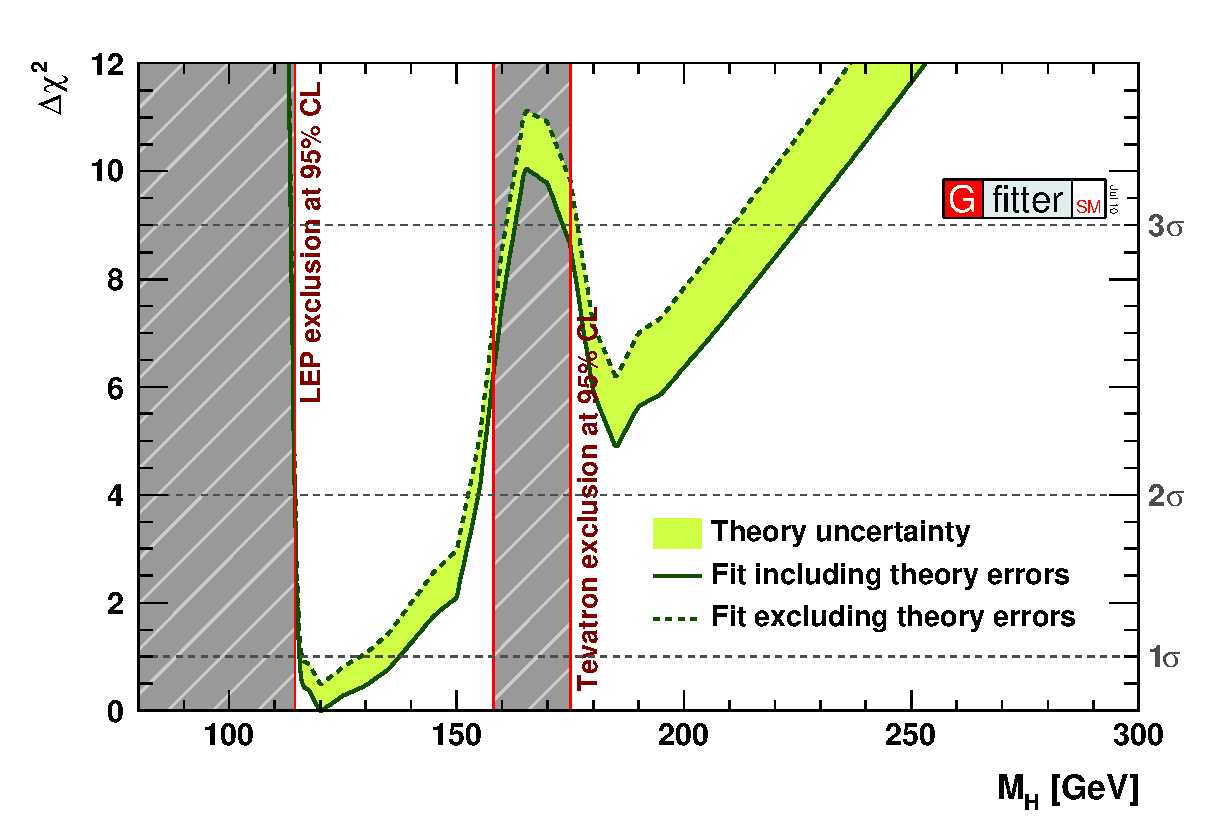
\includegraphics[width=0.495\textwidth]{tex/motivation/ewfit_withdirect}
	\caption{The observed $\Delta\chi^2 = \chi^2 - \chi^2_{\min}$ of electroweak fits 
	versus \mH, neglecting (left) and including (right) results from direct searches
	\cite{Gfitter:2008}. The exclusion limits from LEP and the Tevatron are also shown.
	These results were produced in July 2010. 
	With kind permission from Springer Science and Business Media.}
	\label{fig:ewfit}
\end{figure}

% \begin{figure}
% 	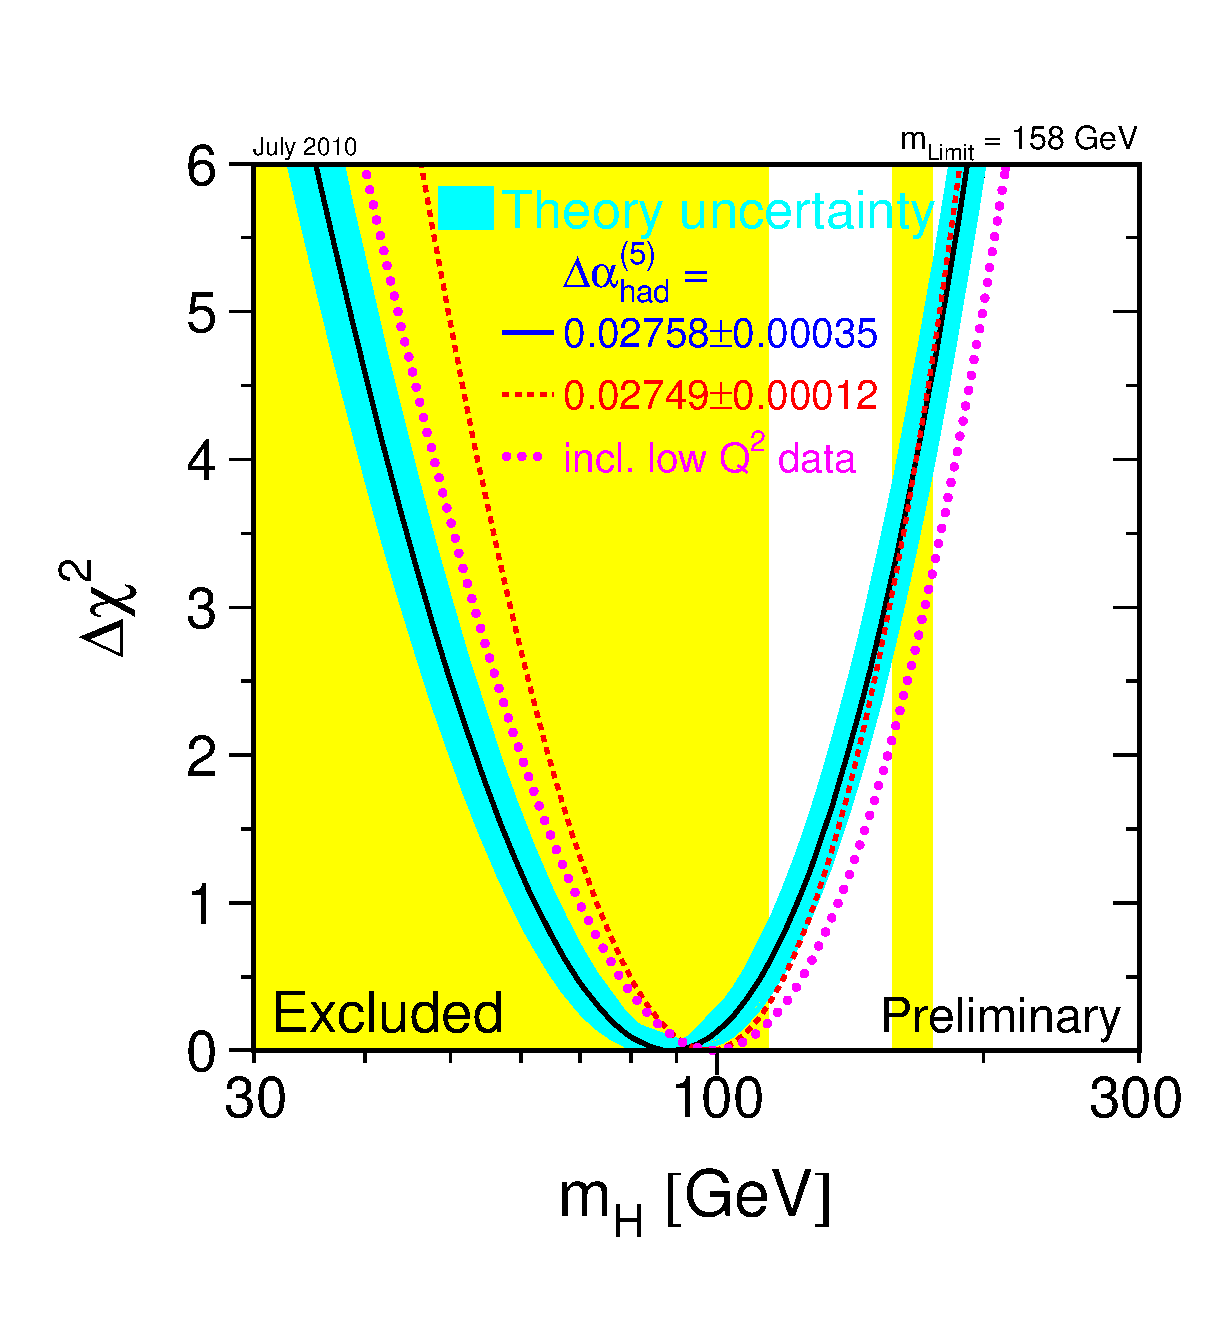
\includegraphics[width=\mediumfigwidth]{tex/motivation/ew_fit_chi2}
% 	\caption{The observed $\Delta\chi^2 = \chi^2 - \chi^2_{\min}$ of electroweak fits 
% 	versus \mH \cite{Grunewald:2010}. The line is fit using \PZ-pole data and direct 
% 	measurements of \mW, $\Gamma_{\PW}$ and $m_{\Ptop}$, and the band is an estimate of 
% 	the uncertainty due to missing higher order corrections. The dashed line uses an 
% 	alternative value of the hadronic vacuum polarisation to show the effect of 
% 	uncertainty in $\alpha(m_{\PZ}^2)$. The dotted line includes low-$Q^2$ experimental 
% 	data. The vertical bands show the 95\% \ac{CL} exclusion limits on \mH arising from 
% 	direct searches at the \ac{LEP} and the Tevatron.}
% 	\label{fig:ewfit}
% \end{figure}



\subsection{Theoretical constraints}
\label{sec:prior_constraints:theory}

Like all coupling constants in a renormalisable theory (see 
\Section~\ref{sec:qcd:renormalisation}), the Higgs quartic coupling $\lambda$ `runs' with 
energy scale $\Lambda$, as described by the renormalisation group equations (RGEs). The 
running is characterised by the $\beta$-function:
\begin{equation*}
	\beta_{\lambda} = \frac{\partial \lambda}{\partial \log\Lambda} \,.
\end{equation*}

For high \mH, self-couplings dominate $\beta_{\lambda}$, which have a
positive contribution. Therefore $\lambda$ increases with the scale, and above some 
critical scale $\Lambda_{\text{c}}$ the EW theory is no longer perturbative. Thus we 
would either expect to observe non-perturbative behaviour at scales 
\about$\Lambda_{\text{c}}$ or new physics at a scale $<\Lambda_{\text{c}}$ that 
circumvents this issue. Larger values of \mH lead to lower values of $\Lambda_{\text{c}}$ 
and are therefore disfavoured (blue line in \Figure~\ref{fig:theory_constraints}). 
Requiring perturbativity up to the reduced Planck scale of 
\unit{$\bar{\Lambda}_{\text{P}}~\about~10^{18}$}{\GeV} (where we expect new physics 
describing gravity) places an upper bound on \mH of \unit{175}{\GeV} \cite{Ellis:2009}.

For small \mH, top loops dominate $\beta_{\lambda}$, which have a negative 
contribution. Therefore $\lambda$ decreases as the scale increases, and above some 
critical scale $\Lambda_{\text{c}}$ the coupling becomes negative. Then the EW 
vacuum is simply a local minimum and it is possible for the Universe to collapse through
quantum tunnelling into the more stable vacuum state (yellow band in 
\Figure~\ref{fig:theory_constraints}). Requiring vacuum stability up to 
$\bar{\Lambda}_{\text{P}}$ places a lower bound on \mH of \unit{129}{\GeV} 
\cite{Ellis:2009}. 
It is also possible to consider a metastable Universe whose expected lifetime is longer 
than its age. Accounting for thermal fluctuations up to temperatures 
\about$\bar{\Lambda}_{\text{P}}$, the EW vacuum has a lifetime longer than the age 
of the Universe if \mH $>$ \unit{122}{\GeV} (pale blue band in 
\Figure~\ref{fig:theory_constraints}) \cite{Ellis:2009}. These bounds are rather 
sensitive to the top mass, which is 
$m_{\Ptop} = \statsyst{173.34}{0.27}{0.71}~\GeV$ \cite{TopMass}.

\begin{figure}[t]
	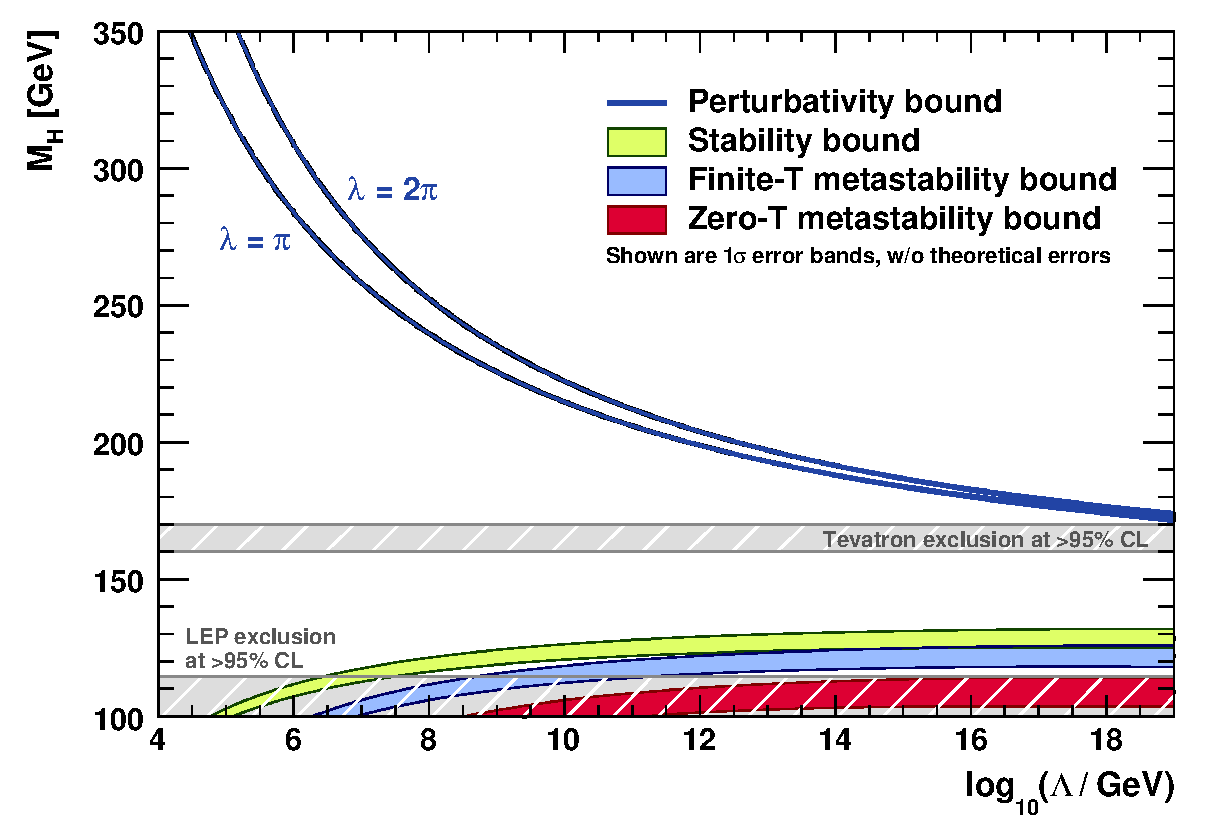
\includegraphics[width=\mediumfigwidth]{tex/motivation/theory_constraints}
	\caption{The scale $\Lambda$ at which the Higgs quartic coupling becomes 
	non-perturbative (blue lines) or an instability in the EW vacuum appears
	(yellow band) \cite{Ellis:2009}. The two blue lines represent different degrees of 
	non-perturbativity (lower line corresponds to a two-loop correction of 25\%, upper 
	line is 50\%), and their difference is indicative of the theoretical uncertainty in 
	this bound. The blue and red bands are bounds for a metastable Universe including and
	neglecting thermal fluctuations respectively. Reprinted from Physics Letters~B \textbf{679}, 4,
	J.~Ellis, J.~R.~Espinosa, G.~F.~Giudice, A.~Hoecker and A.~Riotto, \textit{The Probable 
	Fate of the Standard Model}, 369--375, Copyright (2009), with permission from Elsevier.}
	\label{fig:theory_constraints}
\end{figure}


  \chapter{Computational techniques for the LHC}
    \label{chap:tools}
    %!TEX root = ../../thesis.tex

Although the search for the Higgs boson is motivated by the electroweak interaction, a
detailed knowledge of \ac{QCD} is required to make precise predictions at a hadron-hadron
collider such as the \acs{LHC}. The science of calculating such experimentally verifiable
predictions is known as phenomenology, and this chapter will introduce some of the tools
used in this thesis.

    \section{Quantum chromodynamics}
      \label{sec:qcd}
      %!TEX root = ../../thesis.tex

\ac{QCD} is the theory of the strong interaction, describing coloured particles (quarks 
and gluons) \cite{Ellis:1996}. Two crucial features of \ac{QCD} are \textit{confinement} 
and \textit{asymptotic freedom}. Confinement refers to the observation that quarks and 
gluons are only found within hadrons, and never as isolated states. Asymptotic freedom 
states that, within the hadron, the constituent partons are relatively free to move. Both 
concepts can be understood in terms of a running coupling constant.



\subsection{Renormalisation and the running coupling}
\label{sec:qcd:renormalisation}

When calculating observables within perturbative quantum field theory, ultraviolet (UV) 
divergences are often introduced by Feynman diagrams containing loops. Through careful 
consideration, these UV divergences can be absorbed into renormalised definitions of the 
coupling constant and particle masses. The idea is that the `bare' quantities contain 
compensating divergences, such that the physically measurable quantities are finite:
\begin{equation}
	g_{\text{physical}} = g_{\text{bare}} + \delta g
	\quad\quad\text{and}\quad\quad
	m_{\text{physical}} = m_{\text{bare}} + \delta m
\end{equation}
where $\delta g$ and $\delta m$ are the loop contributions. This procedure is known as 
\textit{renormalisation}.

It is necessary to introduce an unphysical \textit{renormalisation scale} $\mu_R$, above 
which loops are absorbed into renormalised quantities, and below which loops are 
calculated in perturbation theory. Clearly couplings and masses will depend upon $\mu_R$,
though physical observables must not -- however, truncation of the perturbative series 
results in a residual $\mu_R$ dependence. Usually $\mu_R$ is chosen to be the energy 
scale $Q$ of the process under consideration, leading to the concept of a `running 
coupling constant'.

For \ac{QCD}, the coupling constant \alphaS is shown in \Figure~\ref{fig:alpha_s}. At 
small scales (large distances), \alphaS is large and the theory is non-perturbative. 
Though not analytically proven\footnote{
	A mathematically rigorous proof of confinement is one of seven Millennium Prize 
	Problems of the Clay Mathematics Institute, with a bounty of \$1,000,000.
}, confinement has been verified by lattice \ac{QCD} in this regime \cite{Wilson:1974}. 
At high scales (small distances), \alphaS is small -- this is asymptotic freedom 
\cite{Gross:1973,Politzer:1973}. Note that \alphaEM in \acs{QED} exhibits an opposing 
trend, though remains perturbative at accessible energies.
\begin{figure}
	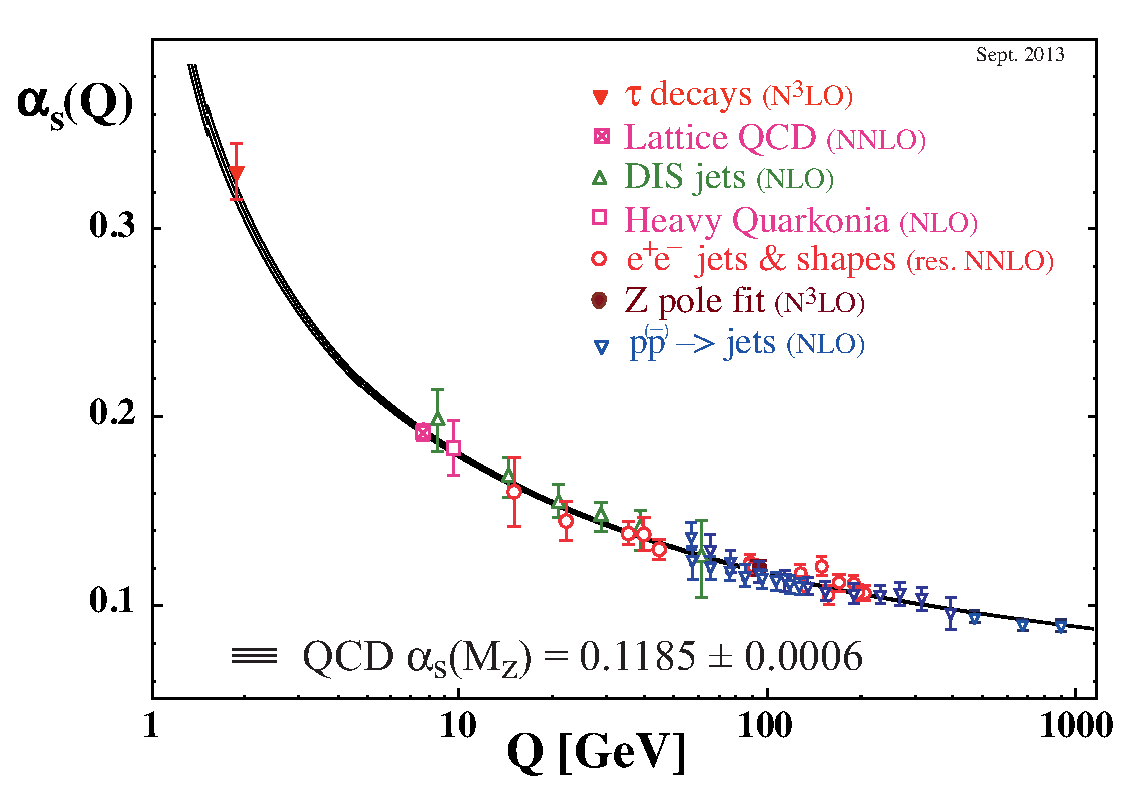
\includegraphics[width=\mediumfigwidth]{tex/tools/alpha_s}
	\caption{The running of the strong coupling constant \alphaS with energy scale $Q$ 
	\cite{PDG:2012}. Experimental measurements at various scales are also shown.}
	\label{fig:alpha_s}
\end{figure}



\subsection{Perturbative QCD}
\label{sec:qcd:pqcd}

Most \acs{LHC} processes of interest involve large momentum transfer where partons are 
asymptotically free. Thus, parton-level cross sections may be calculated with Feynman 
diagrams as a convergent perturbative series in \alphaS
\begin{equation}
	\hat{\sigma} = \sum\limits_{m=0}^{\infty} \alpha_S^{k+m} \hat{\sigma}^{(m)}
\end{equation}
where the hat denotes a parton-level quantity, $k$ is the number of \ac{QCD} vertices at 
tree-level, and $\hat{\sigma}^{(m)}$ is the $m$th order contribution to the cross section.

As mentioned above, the cross section $\hat{\sigma}$ is independent of the 
renormalisation scale
\begin{equation}
	\frac{\d{\hat{\sigma}}}{\d{\mu_R}} = 0 \,.
	\label{eq:xs_rge}
\end{equation}
However, real-life calculations always truncate the series after $n$ terms, leaving a 
residual $\mu_R$ dependence. Inserting the truncated series into (\ref{eq:xs_rge}), we 
find that
\begin{equation}
	\frac{\d{}}{\d{\mu_R}} \sum\limits_{m=0}^{n} \alpha_S^{k+m} \hat{\sigma}^{(m)}
	= \ofOrder{\alpha_S^{k+n+1}}
\end{equation}
and it follows that the residual $\mu_R$ dependence can be used to probe the effect of 
missing higher order terms in the series.

In addition to the UV divergences handled by renormalisation, infrared (IR) divergences 
arise from the soft and collinear emission of massless gluons. However, the 
Kinoshita-Lee-Nauenberg theorem states that these will cancel with IR divergences in 
corresponding loop diagrams \cite{Kinoshita:1962,Lee:1964}.



\subsection{Parton shower}
\label{sec:qcd:ps}

\subsection{Parton distribution functions}
\label{sec:qcd:pdf}

dependence on muF is DGLAP equation

\begin{equation}
	\sigma_{\HepProcess{\Pproton \Pproton \HepTo X}}\parenths{P_1, P_2} = 
	\sum\limits_{a, b} \! \int \! \d{x_1} \d{x_2} \,
	f_a \parenths{x_1, \mu_F^2} f_b \parenths{x_2, \mu_F^2} \,
	\hat{\sigma}_{\HepProcess{ab \HepTo X}} \parenths{p_1, p_2, \alphaS\parenths{\mu_R^2}, \frac{Q^2}{\mu_F^2}, \frac{Q^2}{\mu_R^2}} 
\end{equation}

    \section{Monte Carlo event generation}
      \label{sec:mc}
      %!TEX root = ../../thesis.tex

Monte Carlo (MC) event generators provide a fully-exclusive hadron-level simulation of 
\pp collision events at the LHC \cite{MCnet:general}. This section will describe the 
basic features of a simulated event, before discussing some more advanced techniques 
that shall be used throughout the thesis.



\subsection{The anatomy of an event}

\Figure~\ref{fig:mcevent} shows how the MC event generation is factorised into 
several components, each describing a certain regime of momentum transfer.

\begin{figure}[p]
	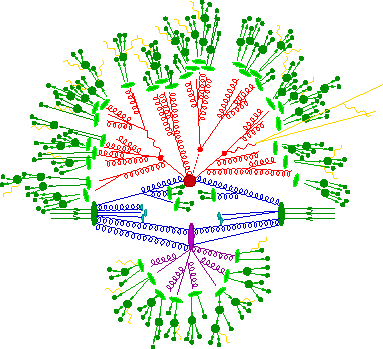
\includegraphics[width=\hugefigwidth]{tex/tools/event}
	\caption{Schematic diagram of a simulated \ttH event, showing how factorisation allows 
	the physics at different scales of momentum transfer $Q$ to be treated independently 
	\cite{MCnet:MatchingLectures}.
	At high-$Q$ is the hard scatter (red circle). As the scale evolves down, partons are 
	radiated in the initial state (blue) and final state (red). At low-$Q$, incoming 
	partons are confined to the beam protons, while outgoing partons hadronise (green 
	blobs). The underlying event comprises multiple partonic interactions (purple blob) 
	and beam remnants (blue blobs). Photons and leptons (yellow) are also radiated.}
	\label{fig:mcevent}
\end{figure}

\begin{description}
\item[Hard scatter] \hfill \\
	The high scale process can be selected as desired (\eg Higgs boson production via 
	gluon-gluon fusion). The relevant parton-level matrix elements (MEs) are calculated 
	using fixed order perturbative QCD, either by the event generator itself or an 
	external program. Historically, these MEs were usually LO, though improvements are 
	discussed in Sections~\ref{sec:mc:merging} and \ref{sec:mc:matching}.
\item[Parton distribution functions (PDFs)] \hfill \\
	Incoming parton momenta are sampled from a proton PDF, usually probed at the 
	scale of the hard scatter ($\muf = Q$). The LHAPDF interface \cite{LHAPDF} provides 
	access to the PDFs of several fitting collaborations, such as CTEQ \cite{CTEQ}, 
	MSTW \cite{MSTW} and NNPDF \cite{NNPDF}. PDFs differ because they are fit with 
	different subsets of experimental data, massive quark treatments, parametrisation 
	models and $\alphaS \parenths{\mZ}$ values.
\item[Final state radiation (FSR)] \hfill \\
	Soft and collinear radiation from outgoing partons is simulated by a universal parton 
	shower, evolving the scale from the hard scatter to the hadronisation scale of 
	\about\unit{1}{\GeV}. The successive emissions are ordered to avoid double-counting --
	typical order parameters are virtuality, transverse momentum and opening angle.

	For the correct treatment of soft emissions, it is vital to preserve colour 
	coherence. This is inherent in an angular ordered shower, but must be manually 
	implemented otherwise. Alternatively, a \textit{dipole shower} considers emissions 
	from colour-connected pairs of partons, and is also inherently coherent.
\item[Initial state radiation (ISR)] \hfill \\
	Soft and collinear radiation from incoming partons is similarly described by a parton 
	shower. However, the small probability of evolving two partons with the kinematics 
	required by the hard process necessitates a \textit{backwards evolution}. Thus, the 
	probability that a parton originated from one of higher momentum and lower scale is 
	calculated, rather than an emission probability.
\item[Hadronisation] \hfill \\
	The confinement of partons to hadrons is non-perturbative, and must be described by a 
	hadronisation model. The \textit{string model} stretches strings between colour 
	partners. At some distance it becomes favourable to convert the potential energy to a 
	\HepProcess{\Pquark \APquark} pair, breaking the string. Once there is insufficient 
	energy to create \HepProcess{\Pquark \APquark} pairs, the hadrons `freeze out'. The 
	\textit{cluster model} splits gluons into \HepProcess{\Pquark \APquark} pairs, which 
	group into colourless clusters with a mass spectrum predicted by QCD. These 
	clusters then decay to the physical hadrons. Note that all hadronisation models 
	require tuning to experimental data.
\item[Hadron and \Ptau decays] \hfill \\
	Many of the hadrons produced during hadronisation are unstable, and must be decayed to
	particles that are stable on a detector traversal timescale, while observing 
	conservation laws and measured branching ratios. Similarly, the \Ptau lepton must be 
	decayed, hadronically or leptonically.
\item[Multiple partonic interactions (MPI)] \hfill \\
	The \textit{underlying event} (UE) is the additional soft hadronic activity caused by 
	partons inactive in the hard scatter. It comprises the breakup of the beam remnants 
	and \textit{multiple partonic interactions} (MPI) between the protons. The size of 
	the MPI activity is correlated to the scale of the hard scatter. 

	In order to calculate the number of additional interactions, the spatial distribution 
	of partons within the proton must be modelled, the impact parameter of the \pp 
	collision must be known, and an IR cut-off must be imposed. This requires 
	non-perturbative models that must be tuned to experimental data.
\item[QED radiation] \hfill \\
	Electrically charged particles can emit photons at any stage of the event generation.
\end{description}



\subsection{Summary of event generators}
\label{sec:mc:generators}

Three event generators are commonly used at the LHC, mainly differing in their 
choice of hadronisation and MPI models, and their parton shower order parameter. 
Efforts to rewrite the older Fortran-based programs in \cpp have led to a generation of 
`out-of-date' Fortran programs that are no longer actively developed. Even so, they are 
still in common usage, and so are included in the descriptions below.

\begin{description}
\item[Herwig] \hfill \\
	\fherwig (Fortran) \cite{fHerwig} and \herwigpp (\cpp) \cite{Herwig++} both employ an 
	angular ordered parton shower and a cluster hadronisation model. An MPI model is 
	included in \herwigpp, but in \fherwig this was provided by \jimmy \cite{Jimmy}.
\item[Pythia] \hfill \\
	\pythia{6} (Fortran) \cite{Pythia6} and \pythia{8} (\cpp) \cite{Pythia8} both use a 
	string hadronisation model and an advanced MPI model. \pythia{8} uses a dipole 
	shower ordered in transverse momentum, whereas \pythia{6} offers a choice of 
	virtuality or transverse momentum ordered parton showers with colour coherence 
	implemented manually.
\item[Sherpa] \hfill \\
	\sherpa (\cpp) \cite{Sherpa} uses a dipole shower ordered in transverse momentum, 
	which is convenient for multi-leg merging (see \Section~\ref{sec:mc:merging}). It 
	uses a cluster hadronisation model and an MPI model similar to that of \pythia{8}.
\end{description}



\subsection{Multi-leg merging}
\label{sec:mc:merging}

Although a parton shower excellently describes the emissions of large numbers of soft and 
collinear partons, it fails to accurately model hard and isolated emissions. It can be 
desirable to describe these using fixed order MEs, which are better suited to the 
task. In doing so, a couple of immediate issues arise. First, we require a smooth 
transition from the emissions of an ME to those of the parton shower. Second, each 
ME is inclusive, and attempting to combine MEs of differing multiplicity 
naturally leads to problems of double counting.

By using a merging prescription, such as the CKKW-L algorithm \cite{CKKW,Lonnblad:2002} 
employed by \sherpa or the MLM algorithm \cite{Merging} employed by \alpgen \cite{Alpgen} 
and \madgraph \cite{MadGraph}, it is possible to consistently combine LO matrix 
elements with differing multiplicities, whilst matching to the parton shower correctly. 
This does require the introduction of a merging scale though. This scale separates the 
ME and parton shower descriptions of the emissions, though the details of the 
separation depend upon the merging prescription.



\subsection{NLO matching}
\label{sec:mc:matching}

It is also possible to match an NLO ME to a parton shower, to improve the accuracy
of both the normalisation and distribution of observables \cite{Nason:2012}. Such a 
calculation must include the LO, virtual-loop and real-emission diagrams, while 
mapping smoothly onto the parton shower for soft emissions. There are currently two valid 
matching prescriptions:

\begin{description}
\item[MC@NLO] \hfill \\
	Simply adding a parton shower to an NLO ME introduces double counting of 
	emissions. The \mcatnlo method compensates for this overlap through a correction to 
	the NLO calculation. This renders the ME dependent upon the parton shower 
	used in the MC event generator. It also introduces negatively weighted events.

	Originally implemented in the \mcatnlo program for matching to \fherwig 
	\cite{MCatNLO-Herwig} and \herwigpp \cite{MCatNLO-Herwig++}, the method has now been 
	automated within the \amcatnlo program \cite{aMCatNLO} and extended for use with 
	\pythia{6} and \pythia{8} \cite{MCatNLO-Pythia}. It is now also included in \sherpa.
\item[POWHEG] \hfill \\
	The \powhegmethod method requires the hardest emission to always be generated by 
	the ME. It achieves the correct hard and soft behaviour by convolving the LO
	ME with a modified Sudakov factor, and then reweighting the differential cross 
	section to the NLO result. Thus the ME is independent of the subsequent 
	parton shower. However, if the parton shower is not transverse momentum ordered, it is
	necessary to use truncated and vetoed parton showers to correctly fill the phase 
	space.

	Originally implemented in \powhegbox \cite{Powheg-method,Powheg-method2,PowhegBox}, 
	variants are now also included in \herwigpp and \sherpa.
\end{description}



\subsection{Additional considerations}
\label{sec:mc:other}

\begin{description}
\item[Detector simulation] \hfill \\
	In order to compare MC events to experimental events recorded at the LHC, 
	it is vital to simulate how the outgoing particles interact with the detector. This 
	is also necessary to calibrate the detector response and estimate efficiencies. 
	\geant \cite{GEANT4,ATLAS-simulation} is used to simulate the energy deposition of 
	each particle during its trajectory through the ATLAS detector (see 
	\Chapter~\ref{chap:experiment}). Since long-lived particles will decay \textit{en 
	route}, particles with lifetime \unit{$c\tau > 10$}{\milli\metre} are decayed by 
	\geant rather than the MC generator. The majority of the simulation time is 
	spent modelling the complex calorimeter geometry; in some cases the simulation is 
	performed by \atlfast \cite{Atlfast}, which contains a simplified calorimeter 
	simulation.

	\textit{Digitisation} converts the energy deposition into readout voltages and 
	currents. Following this, the events can be treated like experimental collision 
	events.
\item[Pile-up simulation] \hfill \\
	As described in \Chapter~\ref{chap:experiment}, each LHC bunch crossing can 
	result in soft proton-proton interactions, known as \textit{pile-up}, in addition to 
	the hard process. This obscures the interesting physics and is important to model 
	accurately.

	In-time pile-up (same bunch crossing as the hard process) is modelled by overlaying 
	simulated energy deposits from soft \pp interactions generated with \pythia{8}. The 
	number of overlaid events depends upon the beam conditions (see 
	\Section~\ref{sec:dataset}).

	Out-of-time pile-up (different bunch crossing to the hard process) affects detector 
	sub-systems whose latency is longer than the bunch spacing. For such sub-systems, 
	signals from out-of-time pile-up are overlaid with corresponding time shifts; again 
	this depends on the beam conditions.
\end{description}



\subsection{Parton shower tuning study}
\label{sec:mc:ps_tuning}

When studying MC modelling uncertainties in the ggF process (see \Section~\ref{sec:ggf_mc}), 
a discrepancy was observed at high jet multiplicity between \meps{\powhegbox}{\pythia{8}} 
and \meps{\powhegbox}{\pythia{6}} (see the green and black lines in 
\Figure~\ref{fig:mc:ps_tuning}). It is also observed in other electroweak processes.

\begin{figure}[t]
	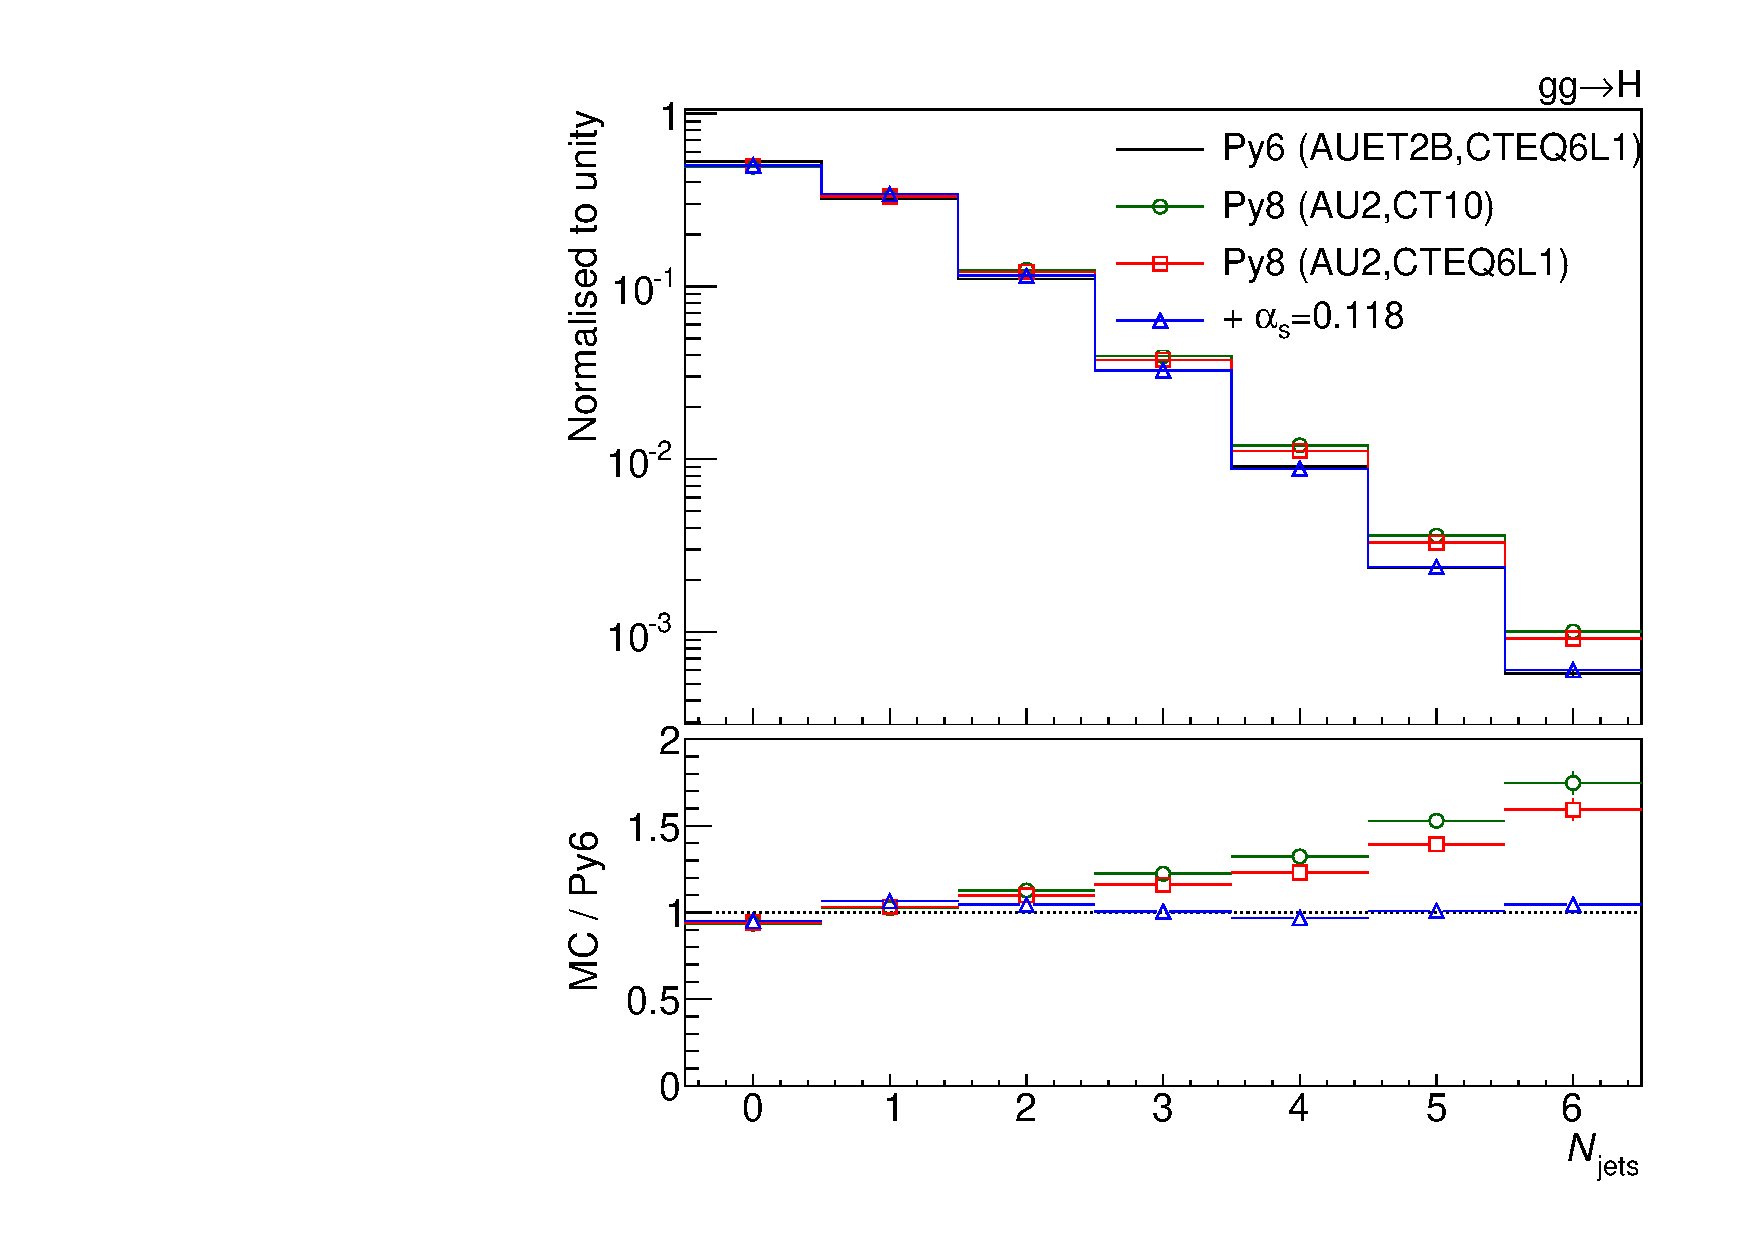
\includegraphics[width=\smallfigwidth]{tex/signal/matching}
	\caption{Jet multiplicity produced by \meps{\powhegbox}{\pythia{8}} with a selection 
	of shower tunes. The green circles correspond to the tune used in the analysis. The red 
	squares change the parton shower PDFs from CT10 to CTEQ6L1. The blue triangles 
	additionally change the parton shower $\alphaS\parenths{\mZ}$ from 0.137 to 0.118 (in 
	agreement with \powhegbox). \meps{\powhegbox}{\pythia{6}} is shown in black for 
	reference, and is in good agreement with \meps{\powhegbox}{\fherwig}.}
	\label{fig:mc:ps_tuning}
\end{figure}

The hadronisation and UE models of standalone \pythia{8} have been tuned to ATLAS 
UE data with a variety of PDF sets (known as AU2 tunes) \cite{ATLAS:tune:2012}.
However, the parton shower was not tuned since the default settings successfully described 
experimental data. 

When modelling ggF with \powhegbox, the AU2-CT10 tune was used in order to match the 
PDFs used in the matrix element calculation. Technically speaking, a dedicated 
\meps{\powhegbox}{\pythia{8}} tune should have been used, but this was unavailable. 
Unfortunately, a couple of issues had a negative impact on the NLO-PS matching. First, 
the parton shower evolves \alphaS at LO, whilst NLO PDFs were used in the shower. 
Second, there was a mismatch between the \alphaS used in \powhegbox, 
$\alphaS\parenths{\mZ} = 0.118$, and the default value in the parton shower, 
$\alphaS\parenths{\mZ} = 0.137$. The effect of these issues is shown in 
\Figure~\ref{fig:mc:ps_tuning}.

Identification of this poor matching has led to improvements in the latest round of MC 
tuning, where dedicated \meps{\powhegbox}{\pythia{8}} tunes are fit using an adjusted 
parton shower \cite{ATLAS:tune:2013}.



    \section{Jet algorithms}
      \label{sec:jets}
      %!TEX root = ../../thesis.tex

We have seen in \Section~\ref{sec:mc} how coloured partons produced in a hard subprocess 
(in the \ac{ME}) or radiated from the incoming partons (\ac{ISR}) will each produce a 
shower of partons, which subsequently hadronise. By measuring the energy and direction of 
the resulting collimated \textit{jet} of hadrons, it is possible to infer information 
about the original quark or gluon. This is very useful for probing the perturbative hard 
scatter.

A \textit{jet algorithm} defines how the large number of final state particle four-momenta 
are grouped into a small number of jet four-momenta. Such an algorithm should satisfy a 
number of criteria, the most important being infrared and collinear safety 
\cite{Salam:2010}. This requires that the jets are insensitive to additional soft or 
collinear emissions.

Multiple jet algorithms are implemented in the \fastjet software library \cite{FastJet}. 
In particular, \textit{sequential recombination algorithms} are popular at the \acs{LHC}, 
which iteratively combine the closest pair of particles according to some distance measure 
$d_{ij}$. 

Consider an algorithm where all the inter-particle distances $d_{ij}$ and particle-beam 
distances $d_{i\text{B}}$ are calculated. If the minimum is a $d_{ij}$, then particles $i$ 
and $j$ are combined into single new particle. If the minimum is a $d_{i\text{B}}$, then 
particle $i$ is declared a jet and removed from the list of particles. Then the algorithm 
restarts. We define the distances
\begin{equation}
	d_{ij} &= \min\parenths{p^{2m}_{\text{T}i}, p^{2m}_{\text{T}j}} \frac{\Delta R^2_{ij}}{R^2} \,,
	&& \Delta R^2_{ij} = \parenths{y_i - y_j}^2 + \parenths{\phi_i - \phi_j}^2 \\
	d_{i\text{B}} &= p^{2m}_{\text{T}i}
\end{equation}
where $p_{\text{T}i}$, $y_i$ and $\phi_i$ are the transverse momentum, rapidity and 
azimuthal angle of particle $i$ with respect to the beam axis, respectively. $R$ and $m$ 
are parameters of the algorithm, with $R$ effectively determining the size of the jet.

With $m=1$, known as the $k_{\text{T}}$ algorithm, combinations between soft particles are 
favoured. This follows the evolution of \ac{QCD}, but leads to rather irregular jet shapes.

With $m=-1$, known as the \antikt algorithm \cite{antikt}, combinations between hard 
particles are favoured. This means the jets grow outwards from a hard `seed', ultimately 
producing more circular jets. However, the jet substructure can no longer be used to infer 
details of the jet evolution history. The jets used in this thesis were \antikt jets with 
$R=0.4$, though shall be described in more detail in \Section~\ref{sec:objects:jets}.


  \chapter{The ATLAS experiment}
    \label{chap:experiment}
    %!TEX root = ../../thesis.tex

The ATLAS experiment is a general purpose particle detector operated by a collaboration of 
more than 3000 scientists. It was designed to search for a broad range of new phenomena by 
precisely studying the collisions of high energy protons, which are provided by the 
\ac{LHC} accelerator at CERN, Geneva.

The \ac{LHC} and the \pp collision data it provides are described in \Section~\ref{sec:lhc}
and \Section~\ref{sec:dataset} respectively. Then, the ATLAS detector is described in
\Section~\ref{sec:atlas}.

    \section{The Large Hadron Collider}
      \label{sec:lhc}
      %!TEX root = ../../thesis.tex

The LHC is the world's largest and most energetic particle accelerator. It is 
installed in a \unit{27}{\kilo\metre} tunnel at a mean depth of \unit{100}{\metre} beneath 
the French--Swiss border, which was previously occupied by the Large Electron--Positron 
collider (LEP). It accelerates beams of protons (or lead ions) to high energy and then 
collides them within the ATLAS, CMS, LHCb and ALICE detectors. Although the design 
centre-of-mass (CM) collision energy is \unit{14}{\TeV}, it operated at \unit{7}{\TeV} and 
\unit{8}{\TeV} during Run I, as described in \Section~\ref{sec:dataset}.

The LHC proton beams have humble beginnings as hydrogen molecules in a standard gas 
bottle, before being stripped of their electrons and entering the LHC accelerator 
complex shown in \Figure~\ref{fig:lhc}. The LHC accelerator features 16 
radio-frequency cavities to provide acceleration and restore energy losses, 1232 
dipole magnets to bend the beam into a nearly circular path, 392 quadrupole magnets to 
focus the beam, and many other magnetic components.\footnote{
	Former DG of CERN Christopher Llewellyn Smith chose the magnet colour to resemble Oxford blue.
}
Most of these magnets rely on unprecedented superconducting twin-bore magnet technology 
operating at cryogenic temperatures.

\begin{figure}[t]
	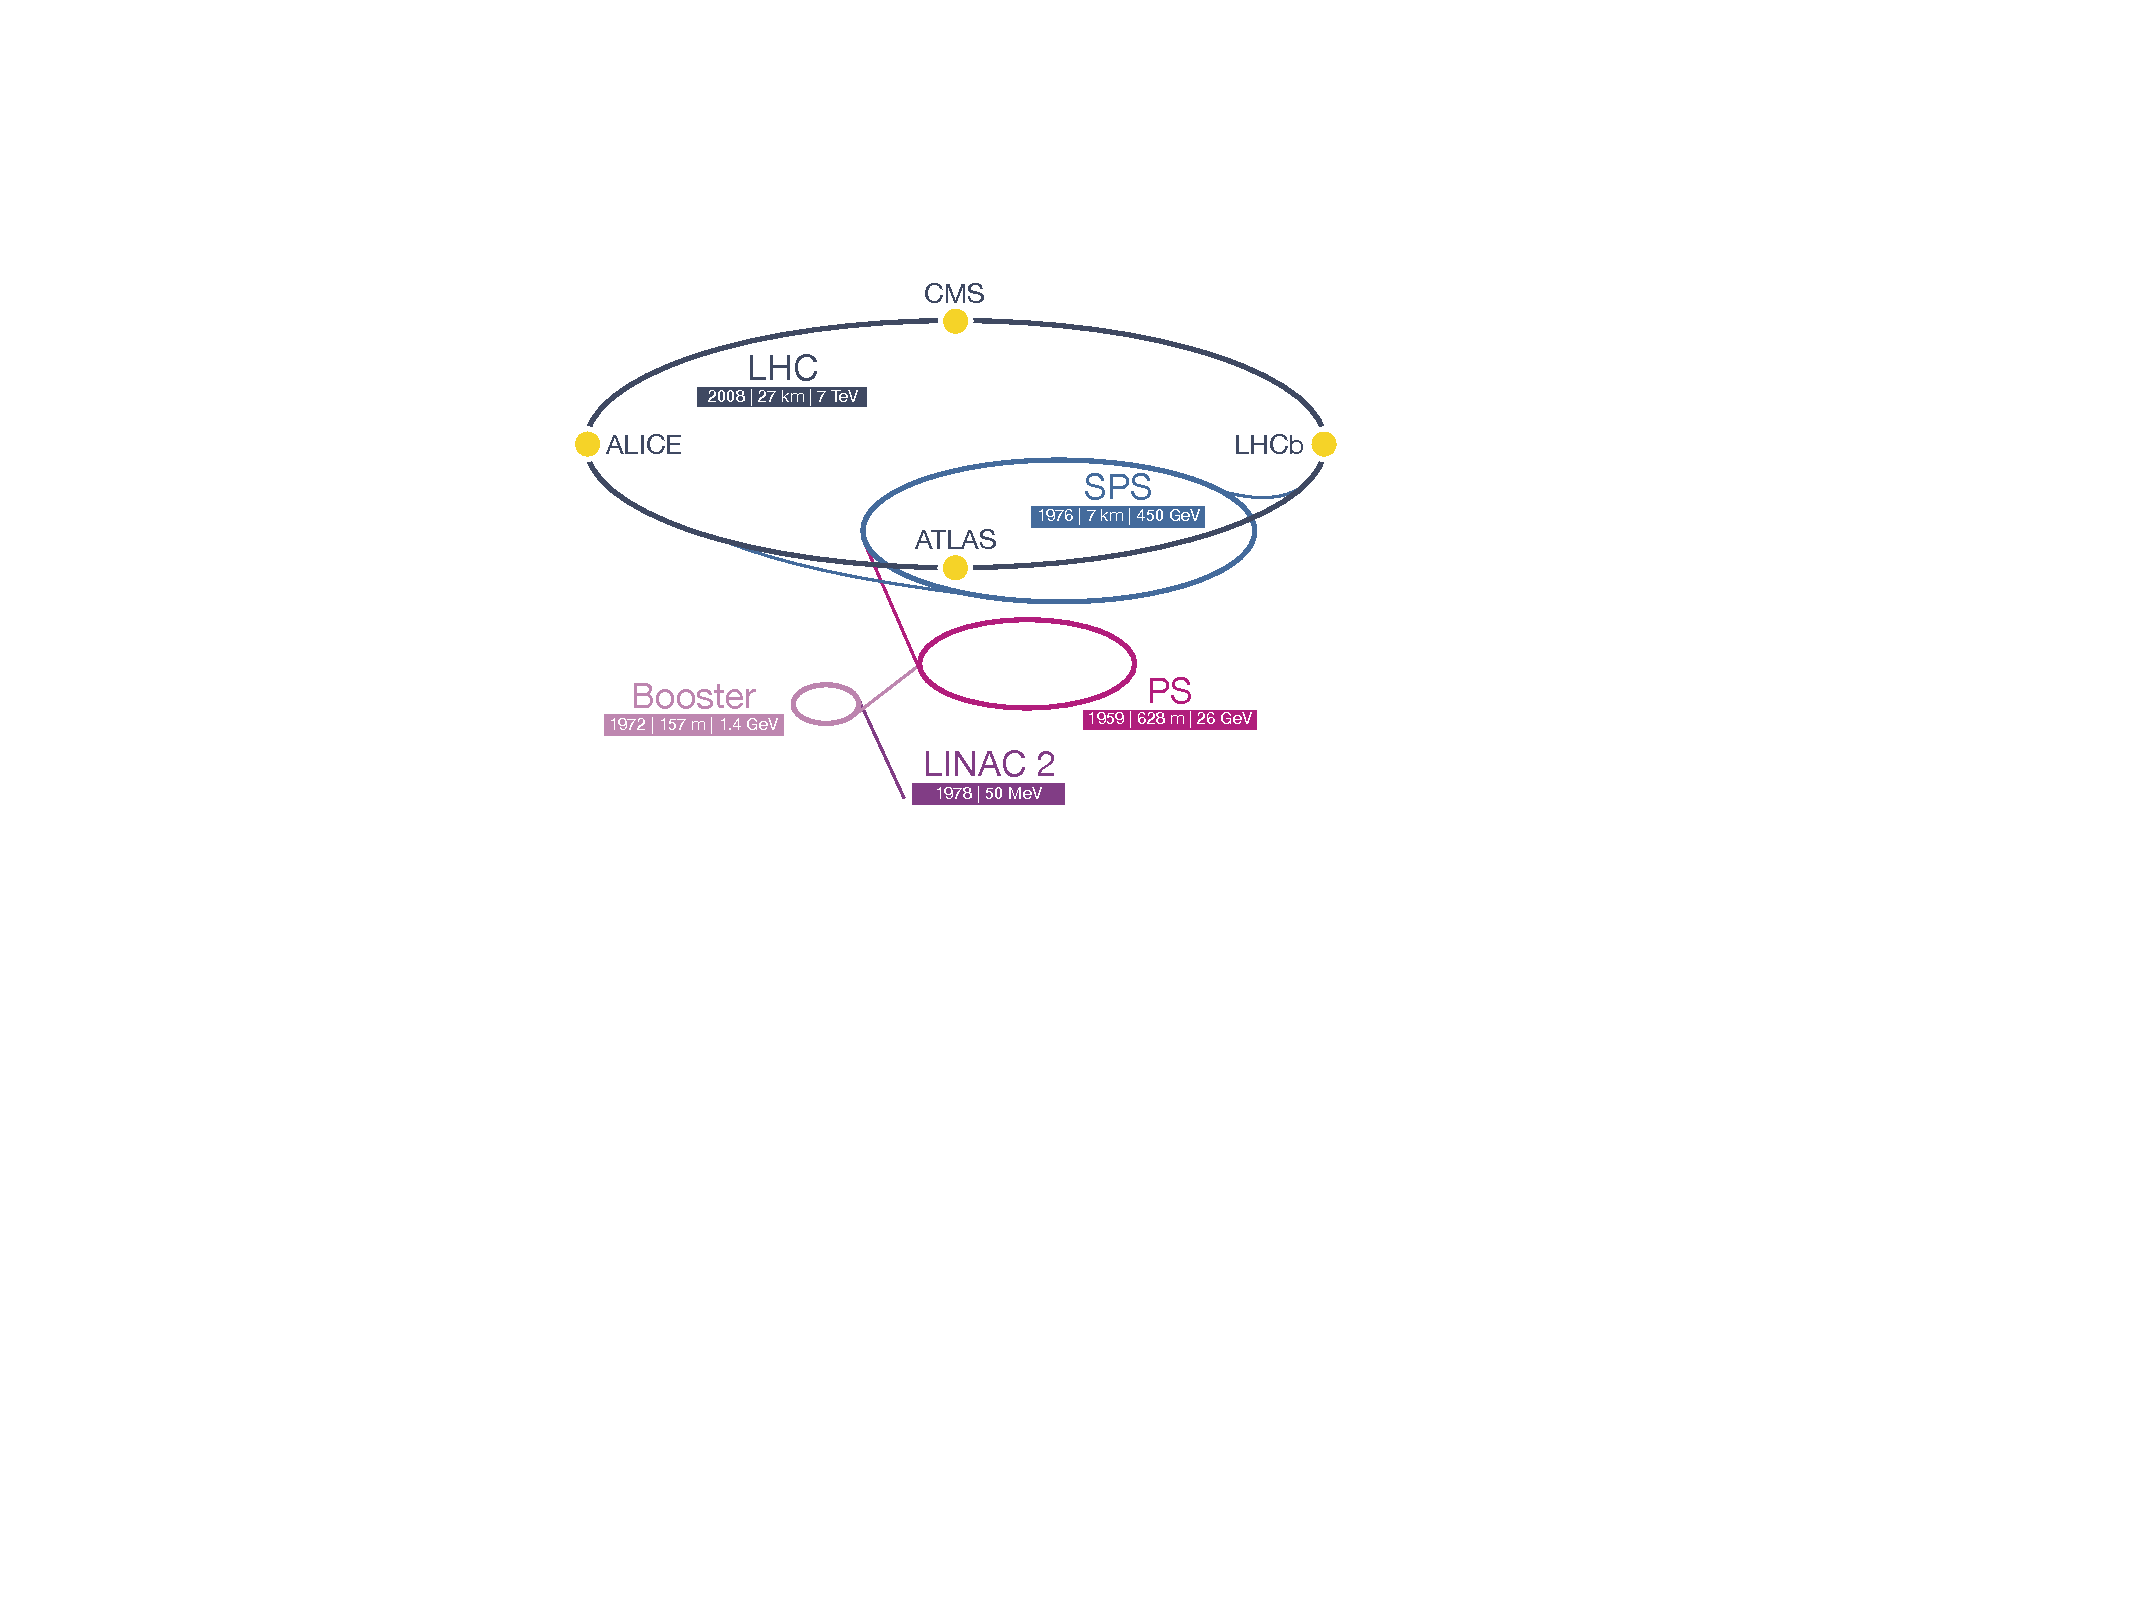
\includegraphics[width=\largefigwidth,clip=true,trim=9.7cm 13.4cm 13.4cm 4.7cm]{custom_images/accelerators}
	\caption{The LHC accelerator complex at CERN. The successively higher energy 
	accelerators are: Linear Accelerator 2 (LINAC 2), Proton Synchrotron Booster, Proton 
	Synchrotron (PS), Super Proton Synchrotron (SPS), and finally the Large Hadron 
	Collider (LHC). The four main LHC detectors are also shown.}
	\label{fig:lhc}
\end{figure}

For experiments to be sensitive to rare processes with small cross sections, such as Higgs 
boson production, the detectors must record a large integrated luminosity. This is seen by 
considering the expected number of events produced for process $i$
\begin{equation}
	N_i = \sigma_i \! \int \! L \, \d{t}
	\label{eq:event_rate}
\end{equation}
where $\sigma_i$ is the cross section and $L$ is the instantaneous luminosity, a figure of 
merit for a collider. The instantaneous luminosity can be increased by optimising the
parameters of
\begin{equation}
	L = \frac{N_{\text{b}}^2 n_{\text{b}} f_{\text{rev}}}{4\pi \varSigma_x \varSigma_y} F
	\label{eq:lumi_beam}
\end{equation}
where $N_{\text{b}}$ is the number or particles per bunch, $n_{\text{b}}$ is the number of 
bunches per beam, $f_{\text{rev}}$ is the revolution frequency, $\varSigma_x$ and 
$\varSigma_y$ are the $x$ and $y$ components of the beam size, and $F$ is a reduction 
factor due to the crossing angle at the interaction point. The LHC is designed to 
hold 2808 proton bunches, corresponding to \unit{25}{\nano\second} bunch spacing, each 
containing $1.15\times10^{11}$ protons. The other design parameters are 
\unit{$\varSigma_{x,y} = 16.7$}{\micro\metre} and \unit{$f_{\text{rev}} = 11.25$}{\kHz}, 
giving a design luminosity of \unit{$L \approx 10^{34}$}{\lumiunits} \cite{LHC}.

A trade-off for higher luminosity is a larger number of additional proton-proton 
interactions, known as \textit{pile-up}. Although a rare interesting event will trigger 
the detector readout, these common uninteresting events will simultaneously be recorded, 
obscuring the interesting physics and degrading detector performance. Increasing 
$N_{\text{b}}$ gives more interactions within the same bunch crossing, known as 
\textit{in-time pile-up}. For large $n_{\text{b}}$, the bunch spacing can be shorter than 
the detector latency, and interactions from other bunch crossings can affect the 
measurement; this is known as \textit{out-of-time pile-up}. Reducing $\varSigma_{x,y}$ 
will increase both types of pile-up.

    \section{\pp collision data}
      \label{sec:dataset}
      %!TEX root = ../../thesis.tex

It is clear from (\ref{eq:event_rate}) that the luminosity delivered to the detector is a 
key input when studying \pp collisions at the LHC. It is directly proportional to the 
expected number of events, and uncertainties in its value will be propagated to measured 
cross sections. The measurement of the luminosity delivered to the ATLAS detector is 
described in \Section~\ref{sec:dataset:lumi}, followed by a description of the dataset 
used in this thesis.



\subsection{Luminosity measurement}
\label{sec:dataset:lumi}

Beam losses incurred by the collisions cause the luminosity to decay (a typical run lasts 
${\approx}10$ hours). Thus, it is necessary to measure the instantaneous luminosity in 
real-time.

At the LHC, the number of inelastic \pp interactions per bunch crossing follows a 
Poisson distribution, with a mean value $\mu$. As mentioned in \Section~\ref{sec:lhc}, 
a large luminosity results in $\mu > 1$ (a condition known as pile-up). Thus, the 
luminosity $L$ can be monitored ``online'' by measuring the observed number of interactions
per crossing $\mu_{\text{vis}}$, using \cite{Lumi2011}
\begin{equation}
	L = \frac{\mu n_{\text{b}} f_{\text{rev}}}{\sigma_{\text{inel}}}
	= \frac{\mu_{\text{vis}} n_{\text{b}} f_{\text{rev}}}{\sigma_{\text{vis}}}
	\label{eq:lumi_measure}
\end{equation}
where $\sigma_{\text{inel}}$ is the inelastic \pp cross section. The expression is 
rewritten with ``visible'' quantities, owing to inefficiencies in the detector and 
algorithm used to measure $\mu$.

The beam conditions monitor (BCM) and LUCID detectors, respectively situated 
\unit{2}{\metre} and \unit{17}{\metre} down the beamline, each count the number of 
activated readout channels per bunch crossing, which is highly correlated with 
$\mu_{\text{vis}}$. The BCM consists of 16 small diamond sensors, and was primarily 
designed to issue beam-abort requests when beam losses risk damaging the ATLAS detector. 
LUCID comprises 16 tubes of C$_4$F$_{10}$ gas, which radiate and collect Cherenkov 
photons when struck by charged particles.

BCM and LUCID are calibrated during dedicated van der Meer (vdM) scans, effectively 
determining $\sigma_{\text{vis}}$ in (\ref{eq:lumi_measure}). In a vdM scan, event rates 
are measured while the beams are separated in steps of known distance, allowing direct 
measurement of beam sizes $\varSigma_x$ and $\varSigma_y$. The absolute luminosity is 
then determined through (\ref{eq:lumi_beam}). The uncertainty in the vdM calibration 
dominates the uncertainty in the delivered luminosity.

Additional methods, such as measuring average particle rates with the ATLAS calorimeters, 
can be used to improve the luminosity estimation offline.



\clearpage
\subsection{Run~I dataset}
\label{sec:dataset:dataset}

Data-taking operations during Run~I of the LHC were incredibly successful, and some 
important parameters of the \pp datasets are summarised in \Table~\ref{tab:dataset} and 
\Figure~\ref{fig:dataset}. These show that a larger dataset was obtained in 2012 compared 
with 2011, but at the expense of a higher pile-up environment.

\begin{table}
	\begin{tabular}{l@{\hskip 0.3in}c@{\hskip 0.3in}c@{\hskip 0.3in}c@{\hskip 0.3in}c}
		\toprule
		& 2010 & 2011 & 2012 & Design \\
		\midrule
		Centre-of-mass energy (\TeV)         & 7 & 7 & 8 & 14 \\
		Minimum bunch spacing (\nano\second) & 150 & 50 & 50 & 25 \\
		Peak luminosity (\unit{$10^{33}$}{\lumiunits}) & 0.2 & 3.6 & 7.7 & 10 \\
		Delivered luminosity (\invfb)       & 0.047 & 5.46 & 22.8 & -- \\
		Recorded luminosity (\invfb)        & 0.044 & 5.08 & 21.3 & -- \\
		Luminosity uncertainty $\delta L/L$ & 3.5\% & 1.8\% & 2.8\% & -- \\
		\bottomrule
	\end{tabular}
	\caption{Summary of \pp collision data during LHC Run~I. Luminosities use the 
	offline calibration.}
	\label{tab:dataset}
\end{table}

\begin{figure}
	\begin{subfigure}[b]{0.495\textwidth}
		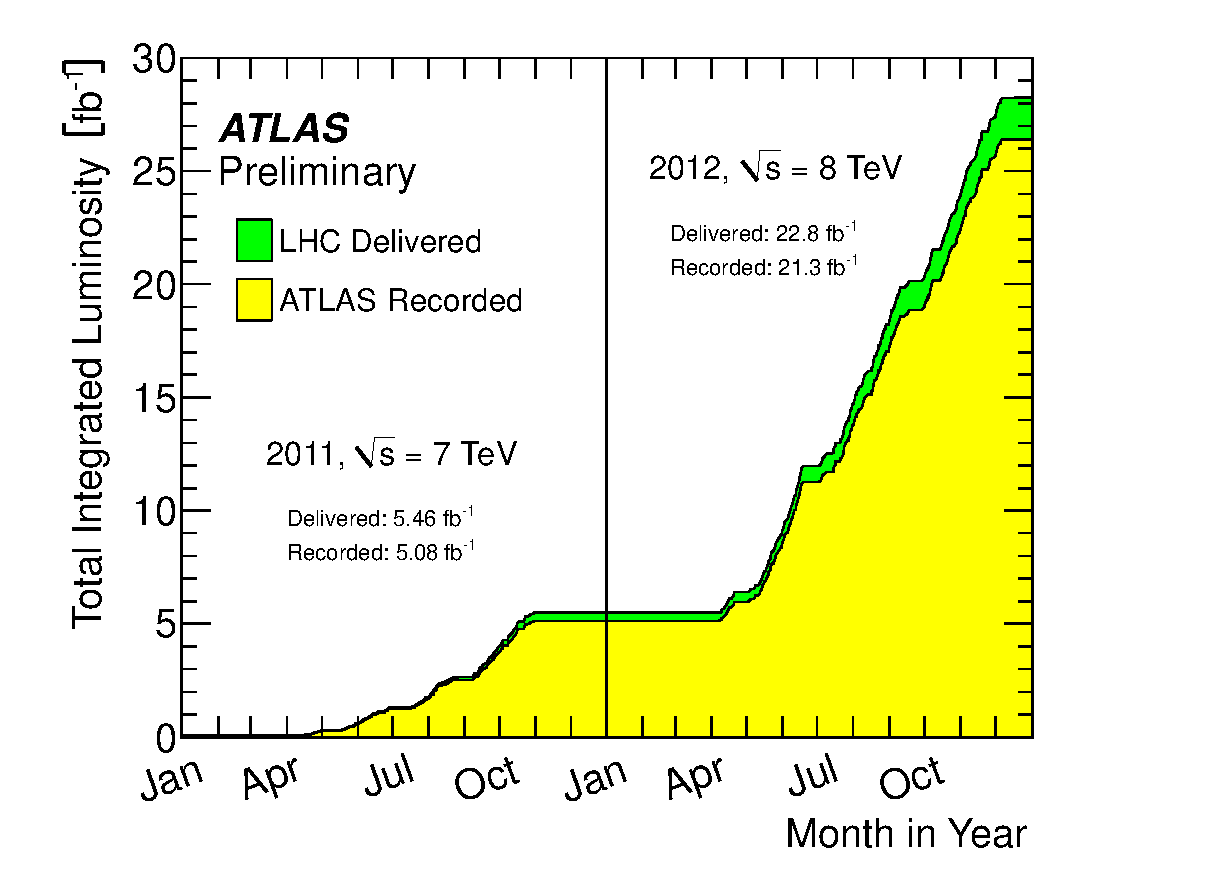
\includegraphics[width=\textwidth]{tex/experiment/luminosity}
		\caption{Luminosity}
		\label{fig:dataset:lumi}
	\end{subfigure}
	\hfill
	\begin{subfigure}[b]{0.495\textwidth}
		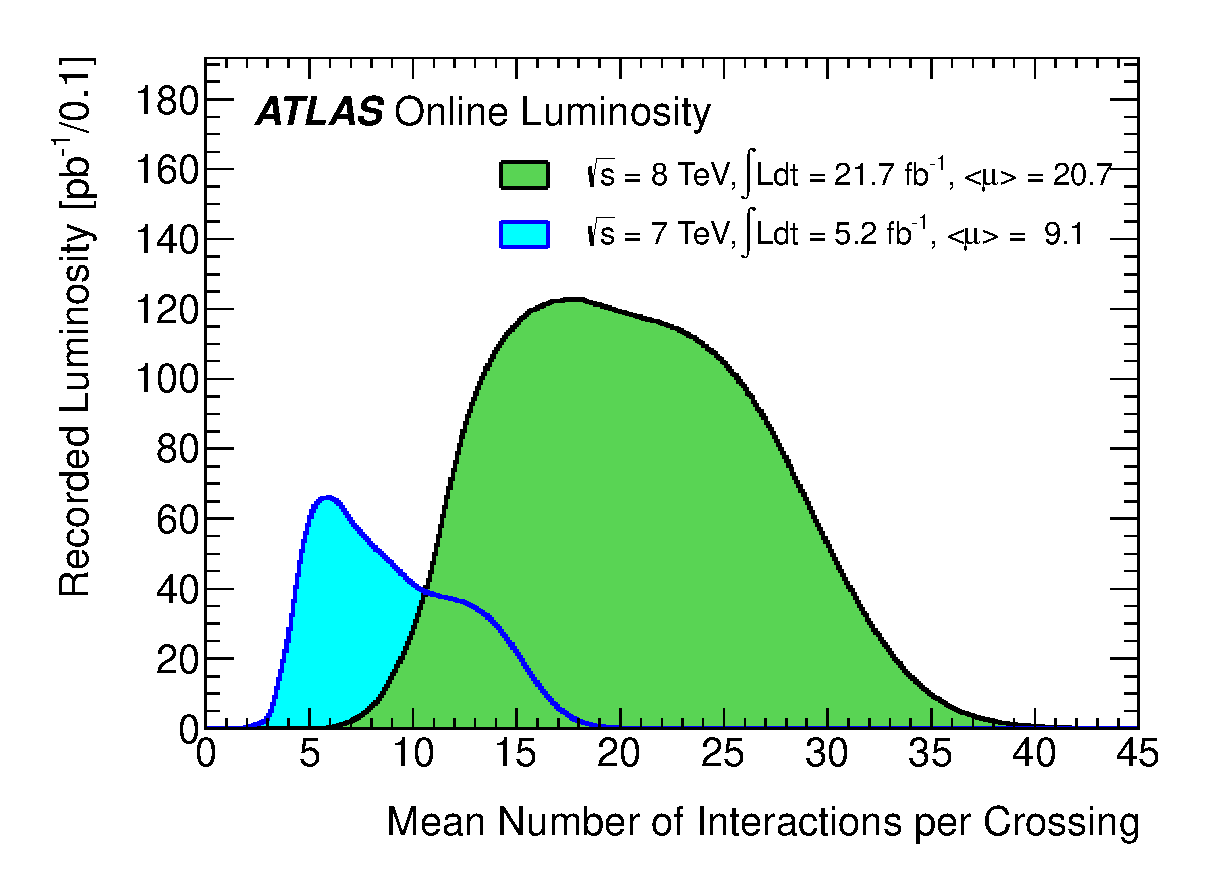
\includegraphics[width=\textwidth]{tex/experiment/pileup}
		\caption{Pile-up}
		\label{fig:dataset:pileup}
	\end{subfigure}
	\caption{(a) Cumulative luminosity delivered (green), recorded (yellow), and declared 
	`good for physics' (blue) during 2011 and 2012. Luminosities use the offline 
	calibration.
	(b) Mean number of interactions per bunch crossing $\mu$ for the 2011 (blue) and 
	2012 (green) datasets, calculated with an inelastic \pp cross section of 
	\unit{71.5}{\milli\barn} at \unit{$\sqrt{s} = 7$}{\TeV} and 
	\unit{73.0}{\milli\barn} at \unit{$\sqrt{s} = 8$}{\TeV}.
	Luminosities use the online calibration.}
	\label{fig:dataset}
\end{figure}


    \section{The ATLAS detector}
      \label{sec:atlas}
      %!TEX root = ../../thesis.tex

ATLAS is a general-purpose particle detector for probing hadron-hadron collisions 
\cite{ATLAS-detector}, from precise measurements of Standard Model (SM) processes to 
searches for signatures of new physics. As such, it must achieve a good performance in 
the reconstruction of all physics objects interacting with the detector (leptons, photons 
and jets), and infer the existence of non-interacting particles through transverse 
momentum imbalance. A good vertex resolution is needed for jet flavour tagging and to 
distinguish pile-up events. Other requirements include a fast trigger system to select 
interesting events to record.

The design of ATLAS exhibits cylindrical and forward-backward symmetries with the nominal 
interaction point at the centre.\footnote{
	ATLAS uses a right-handed coordinate system with its origin at the nominal 
	interaction point. The $x$-axis points to the centre of the LHC ring, the 
	$y$-axis points upwards, and the $z$-axis points along the beam line. Positions and 
	directions within the detector are given in spherical coordinates $(r, \theta, \phi)$ 
	where $r$ is the radial distance, $\theta$ is the polar angle and $\phi$ is the 
	azimuthal angle. Usually the polar angle is replaced with pseudorapidity 
	$\eta = -\ln\tan(\theta/2)$. The distance between two positions in $\eta\mhyphen\phi$ 
	space is $\Delta R = \sqrt{\Delta\eta^2 + \Delta\phi^2}$.
	Observables labelled ``transverse'' are projected into the $x\mhyphen y$ plane.
} 
The three detector sub-systems (tracking, calorimetry and the muon spectrometer) 
follow a consistent design of a central barrel with end-caps at both ends, giving a high 
degree of hermeticity (see \Figure~\ref{fig:atlas_whole}). Barrel components are arranged 
on concentric cylinders around the beam axis, while end-cap components are on disks 
perpendicular to the beam axis.

\begin{figure}
	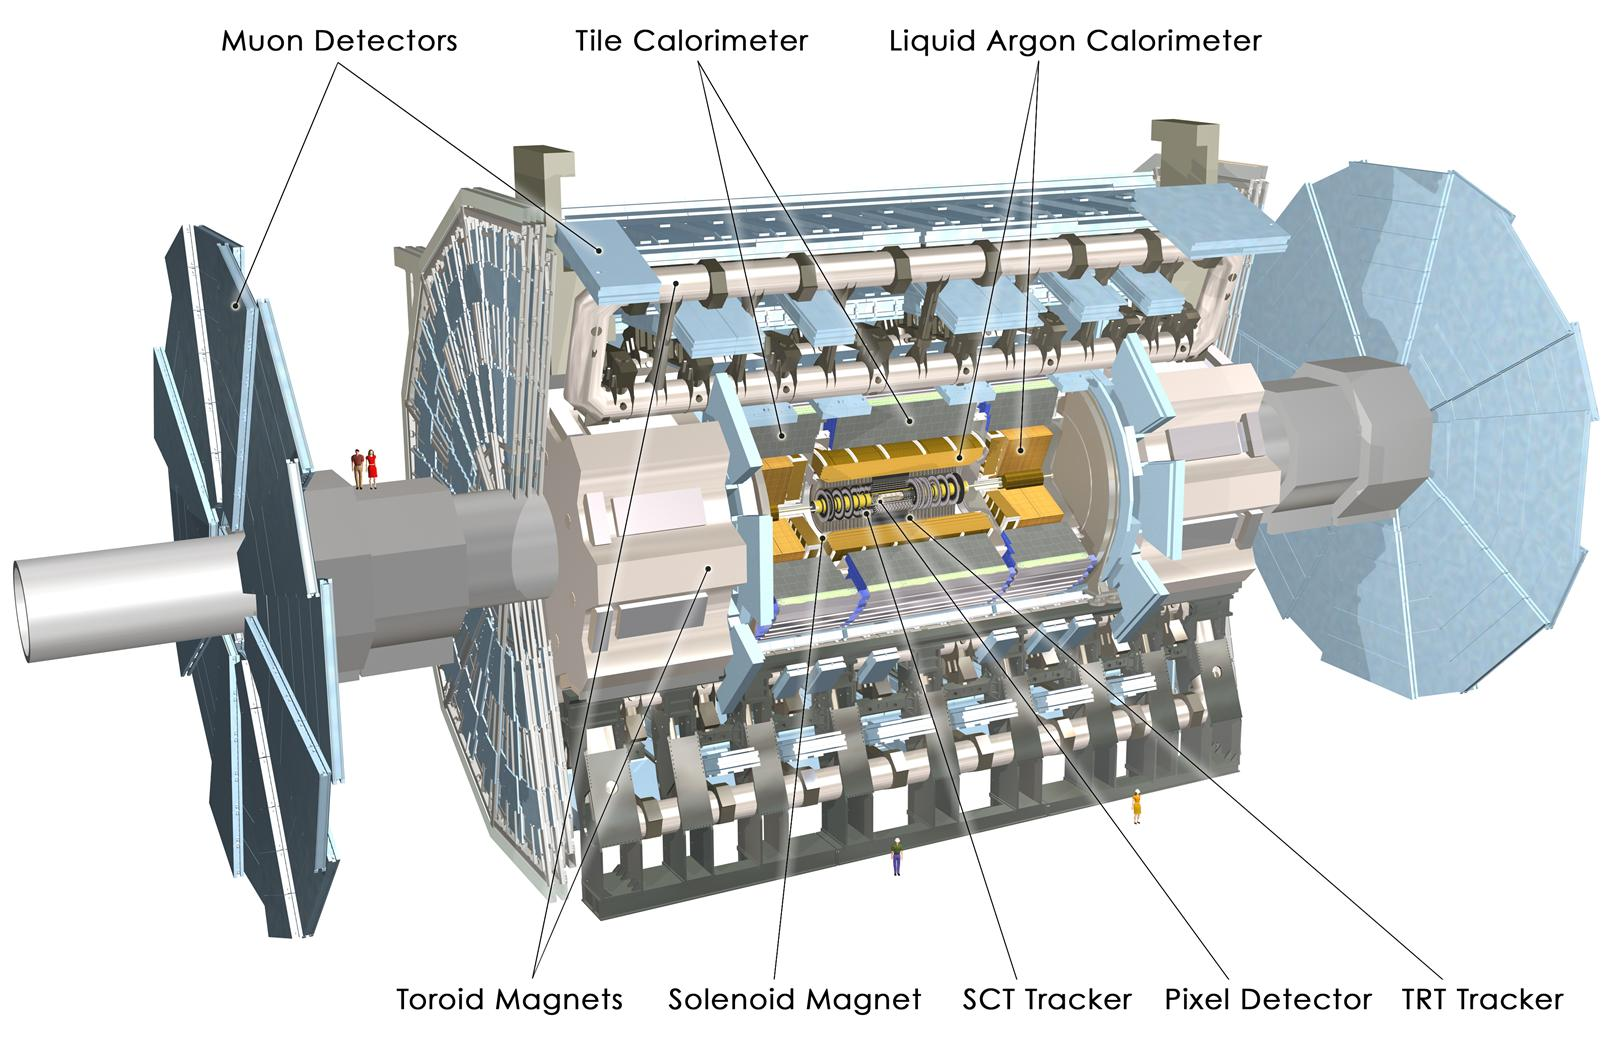
\includegraphics[width=\hugefigwidth]{tex/experiment/atlas_whole}
	\caption{Cut-away view of the ATLAS detector \cite{ATLAS-detector}. It has a height 
	of \unit{25}{\metre}, a length of \unit{44}{\metre} and weighs 7000~tonnes.}
	\label{fig:atlas_whole}
\end{figure}

\Figure~\ref{fig:atlas_wedge} shows how different particles interact with the various 
parts of the detector. Next to the beam pipe is the inner detector which precisely tracks 
the trajectories of charged particles. Then there are the electromagnetic and hadronic 
calorimeters which absorb and measure the energy of interacting particles. Since 
high-\pt muons act as minimum ionising particles, they survive the calorimeters and are 
tracked by the muon spectrometer. Superconducting solenoid and toroid magnets provide 
magnetic fields to the inner detector and muon spectrometer respectively, allowing the 
momenta of charged particles to be measured from the curvature of their tracks.

\begin{figure}
	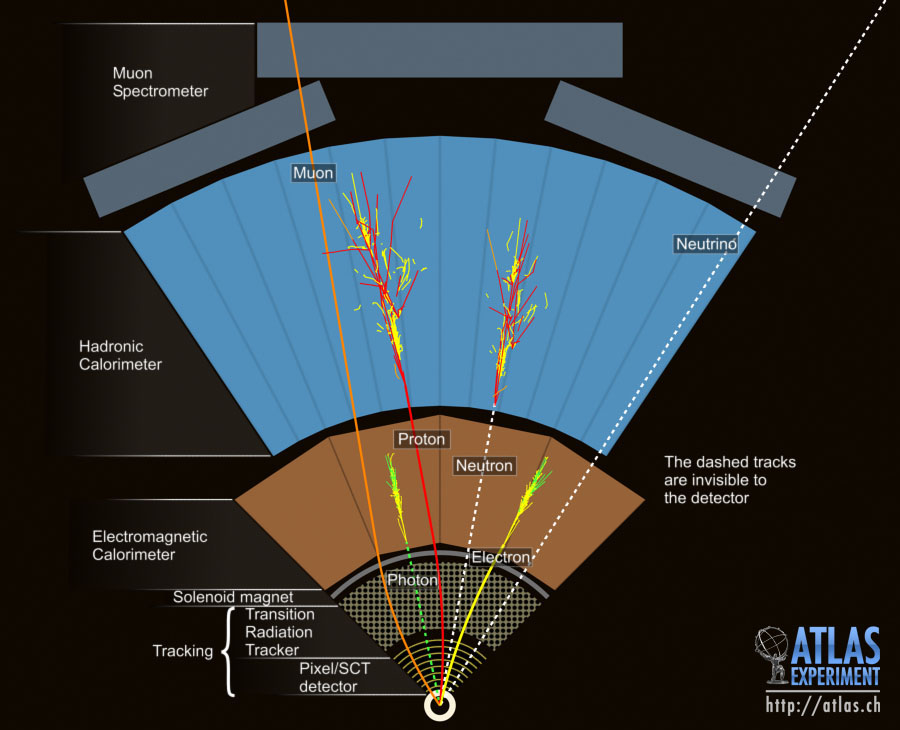
\includegraphics[width=0.98\largefigwidth]{tex/experiment/atlas_wedge}
	\caption{Cross-sectional view of ATLAS, showing how different particles interact with 
	the sub-detectors. ATLAS Experiment \copyright\xspace 2013 CERN.}
	\label{fig:atlas_wedge}
\end{figure}



\subsection{Tracking}
\label{sec:atlas:id}

\begin{figure}[t]
	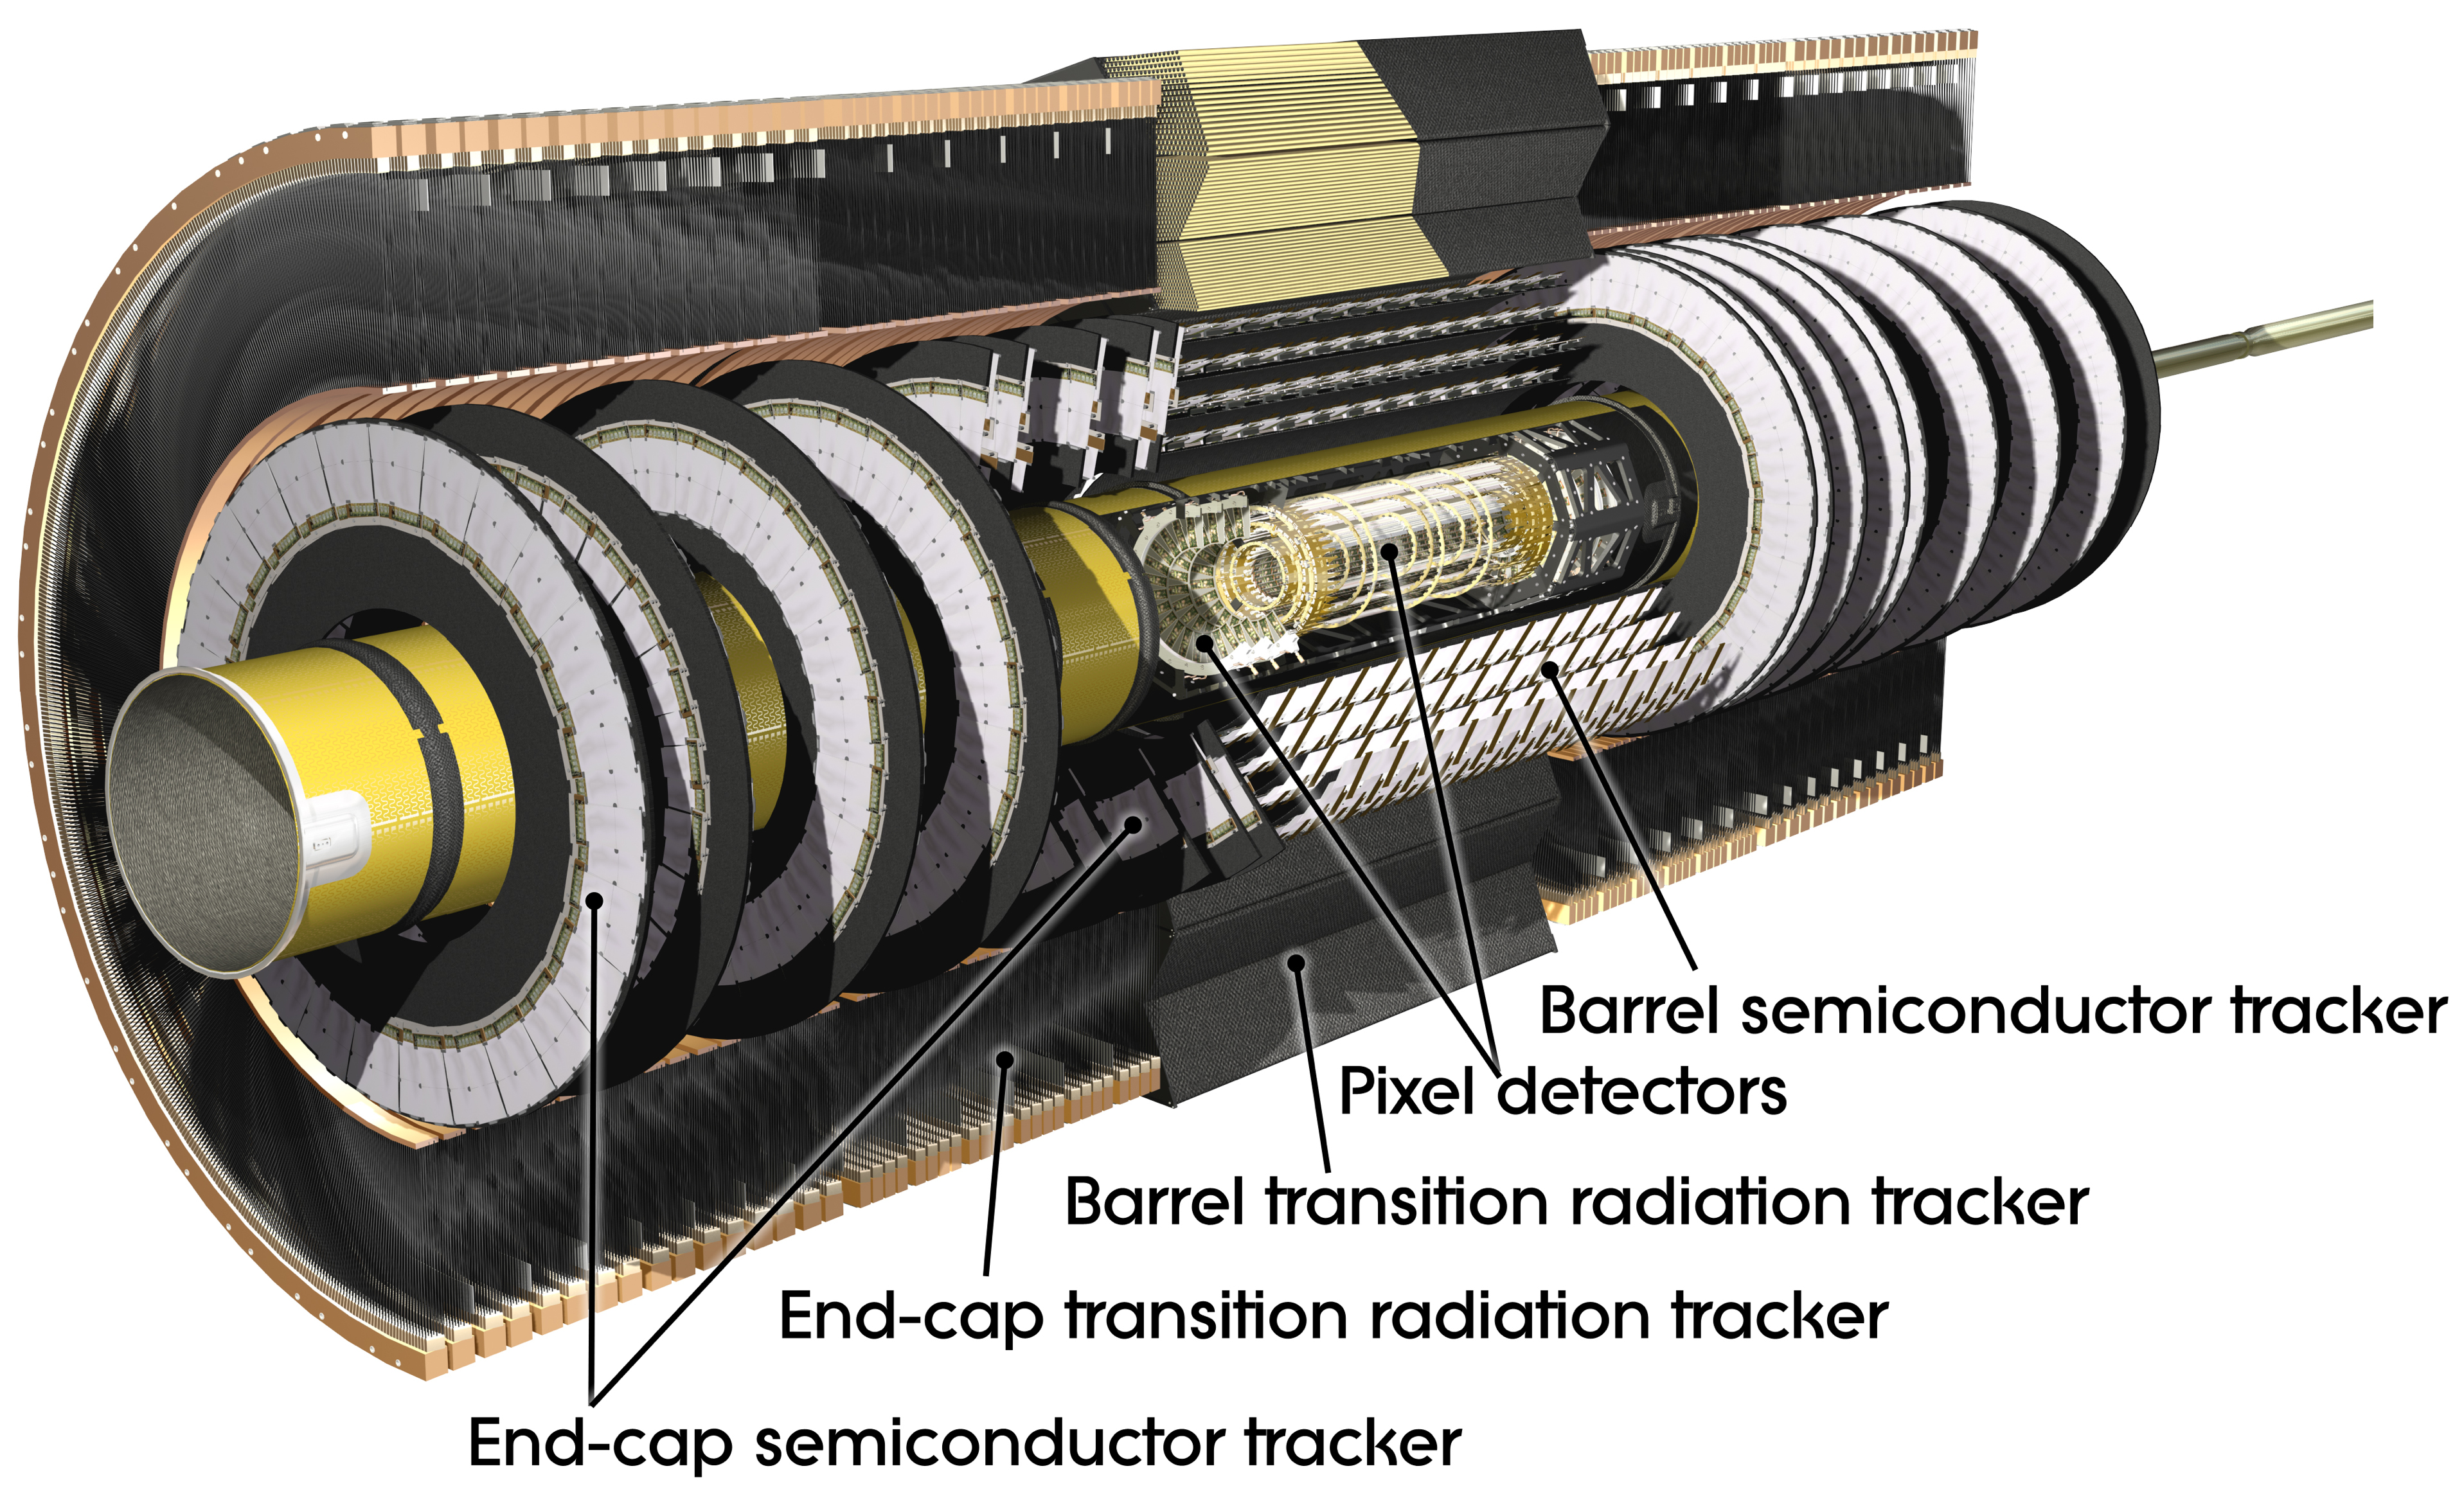
\includegraphics[width=0.55\textwidth]{tex/experiment/id_whole}
	\hfill
	\includegraphics[width=0.44\textwidth]{tex/experiment/id_wedge}
	\caption{The ATLAS inner detector: cut-away view (left) and cross-sectional view 
	showing a trajectory through the three sub-detectors (right) \cite{ATLAS-detector}. 
	The inner detector has a length of \unit{6.2}{\metre} and a radius of 
	\unit{1.1}{\metre}. The beam pipe radius is \unit{29}{\milli\metre}.}
	\label{fig:inner_detector}
\end{figure}

Pattern recognition algorithms are used to precisely track the trajectories of charged 
particles through the inner detector (ID), shown in \Figure~\ref{fig:inner_detector}. The 
ID is immersed in a \unit{2}{\tesla} solenoidal magnetic field, which enables the 
momentum of a particle to be measured from the curvature of its track. Momentum and 
vertex measurements both require an excellent spatial resolution, which is achieved 
through fine detector granularity. The ID covers the region $\mods{\eta} < 2.5$ and 
consists of three complementary sub-detectors:
\begin{description}
\item[Pixel detector] \hfill \\
	The pixel detector is installed in three layers closest to the beam pipe, and 
	therefore requires the highest granularity to handle the large particle fluxes.
	It comprises more than 80 million silicon pixels, each of area 
	\unit{$50 \times 400$}{\micro\metre\squared} and thickness \unit{250}{\micro\metre}. 
	The intrinsic accuracy is \unit{10}{\micro\metre}$\,\times\,$\unit{115}{\micro\metre} 
	in $r\phi \mhyphen z$ ($r\phi \mhyphen r$) space in the barrel (end-cap).

	A silicon particle detector consists of a reverse-biased p-n junction. When a charged
	particle passes through the depletion region it creates an electron-hole pair, which 
	travel to the respective electrodes and produce a signal current.
\item[Semiconductor tracker (SCT)] \hfill \\
	The SCT features 15,912 silicon strip sensors, each consisting of 770 strips 
	with a pitch of \unit{80}{\micro\metre} and a length of \unit{6}{\centi\metre}. Pairs 
	of sensors are sandwiched together into modules with a stereo angle of 
	\unit{40}{\milli\radian}, enabling the coordinate parallel to the strip to be 
	measured. There are four (nine) layers of modules in the barrel (end-cap), which 
	ensures that each track passes through at least four modules. 
	The intrinsic accuracy is \unit{17}{\micro\metre}$\,\times\,$\unit{580}{\micro\metre} 
	in $r\phi \mhyphen z$ ($r\phi \mhyphen r$) space for the barrel (end-cap).
\item[Transition radiation tracker (TRT)] \hfill \\
	The TRT features 370,000 drift chambers, known as straws, which simultaneously 
	function as a straw tracker to enhance particle tracking and as a transition 
	radiation detector to aid electron identification. Straws are aligned with the beam 
	pipe in the barrel and radially in the end-caps. The TRT covers the region 
	$\mods{\eta} < 2.0$.

	Each \unit{4}{\milli\metre} diameter straw has a 
	Kapton\textsuperscript{\circledR}\xspace wall with a conductive coating, which 
	acts as a cathode at \unit{$-1530$}{\volt}, and a central tungsten wire anode. The 
	straws are filled with a xenon-based gas mixture that is ionised by a traversing 
	charged particle. The freed electrons drift to the anode and produce a signal current.
	The drift time is used to measure the impact parameter of the incident charged 
	particle relative to the anode and, since a track typically traverses 36 straws, 
	collectively this information yields an intrinsic accuracy of \unit{130}{\micro\metre}
	in $r\phi$ (much smaller than the straw diameter). However, there is no tracking 
	information parallel to the straw.

	The layers of straws are interleaved with polypropylene radiator fibres or foils, and 
	the changes in refractive index cause charged particles to emit X-ray transition 
	radiation (TR). The TR is absorbed by the xenon gas in the straws; TR signals are 
	distinguished from tracking signals by a higher threshold. Since the probability of 
	TR is proportional to the particle's $\gamma$-factor, for a given energy lighter 
	particles produce more TR than heavier particles. This aids electron-pion 
	discrimination.
\end{description}



\subsection{Calorimetry}
\label{sec:atlas:calo}

Particle energies are measured with sampling calorimeters, which consist of alternating 
layers of absorber and active material. The dense absorber causes energy deposition 
via a particle shower, whilst the active material produces a signal proportional to the 
sampled energy. The length scale of energy loss is the radiation length $X_0$ for 
electrons and photons\footnote{
	High-energy electrons (photons) mostly lose energy in matter by bremsstrahlung 
	(\epluseminus pair production). In this regime, $X_0$ is (a) the mean distance in 
	which an electron loses all but $\eexp{-1}$ of its energy, (b) $\tfrac{7}{9}$ of the 
	mean free path of a photon, and (c) the characteristic scale of electromagnetic 
	showers.
} and the nuclear interaction length $\lambda$ for hadronic showers\footnote{
	Hadrons lose energy in matter through inelastic hadronic interactions, forming hadronic showers (though neutral pions create electromagnetic showers). $\lambda$ is 
	(a) the mean free path of a hadron, and (b) the characteristic scale of hadronic showers.
}, while muons act as minimum ionising particles and escape the calorimeters. Since 
punch-through into the muon system must be minimised, $X_0$ and $\lambda$ set the size of 
the calorimeter. Conversely, limits to detector size constrain the materials that can be
used.

\begin{figure}[t]
	\includegraphics[width=\largefigwidth]{tex/experiment/calo_whole}
	\caption{Cut-away view of the ATLAS calorimeter system \cite{ATLAS-detector}.}
	\label{fig:calorimeters}
\end{figure}

The ATLAS calorimeter consists of an inner electromagnetic calorimeter (for electrons and 
photons) and an outer hadronic calorimeter (for jets), as shown in 
\Figure~\ref{fig:calorimeters}. They cover the regions $\mods{\eta} < 3.2$ and 
$\mods{\eta} < 4.9$ respectively. The total thickness of the electromagnetic calorimeter 
corresponds to more than $22 X_0$ and the total thickness of the entire calorimeter 
corresponds to more than $10 \lambda$.
\begin{description}
\item[Electromagnetic calorimeter (ECal)] \hfill \\
	The ECal uses a lead absorber and a liquid argon (LAr) active material arranged 
	in an accordion geometry, which ensures uniform $\phi$-coverage. The LAr is ionised 
	by charged particles, and the freed electrons produce a signal current in the readout 
	electrodes. LAr was chosen for its linear behaviour, stability and radiation-hardness.

	A fine granularity is required to make precise electron and photon measurements, and 
	to distinguish single photons from $\HepProcess{\Ppizero \HepTo \Pphoton \Pphoton}$. 
	Thus, the ECal is typically segmented into three layers with a minimum 
	$\Delta\eta\times\Delta\phi$ granularity of $0.003 \times 0.025$. The transition 
	between the barrel and the end-cap, $1.37 < \mods{\eta} < 1.52$, is used for detector 
	services. Since this material is difficult to model, this ``crack'' region is usually 
	excluded when reconstructing electrons.

	For $\mods{\eta} < 1.8$, a LAr presampler is installed before the first lead layer. 
	This enables estimation of the energy lost by electrons and photons before 
	encountering the ECal.
\item[Hadronic calorimeter (HCal)] \hfill \\
	The HCal consists of a tile calorimeter covering $\mods{\eta} < 1.7$, a hadronic 
	end-cap (HEC) covering $1.5 < \mods{\eta} < 3.2$, and a forward calorimeter (FCal) 
	covering $3.1 < \mods{\eta} < 4.9$. The HCal has a coarser granularity than the
	ECal: it is typically segmented into three layers with a minimum 
	$\Delta\eta\times\Delta\phi$ granularity of $0.1 \times 0.1$.

	The tile calorimeter uses a steel absorber with scintillator tiles as the active 
	material. The scintillation light is collected by optical fibres and turned into a 
	signal by photomultiplier tubes. The HEC and FCal both use LAr active material.
	The HEC uses a copper absorber, whereas the FCal uses copper in the first layer (for 
	electromagnetic measurements) and tungsten in the two subsequent layers.
\end{description}



\subsection{Muon spectrometer}
\label{sec:atlas:ms}

\begin{figure}[t]
	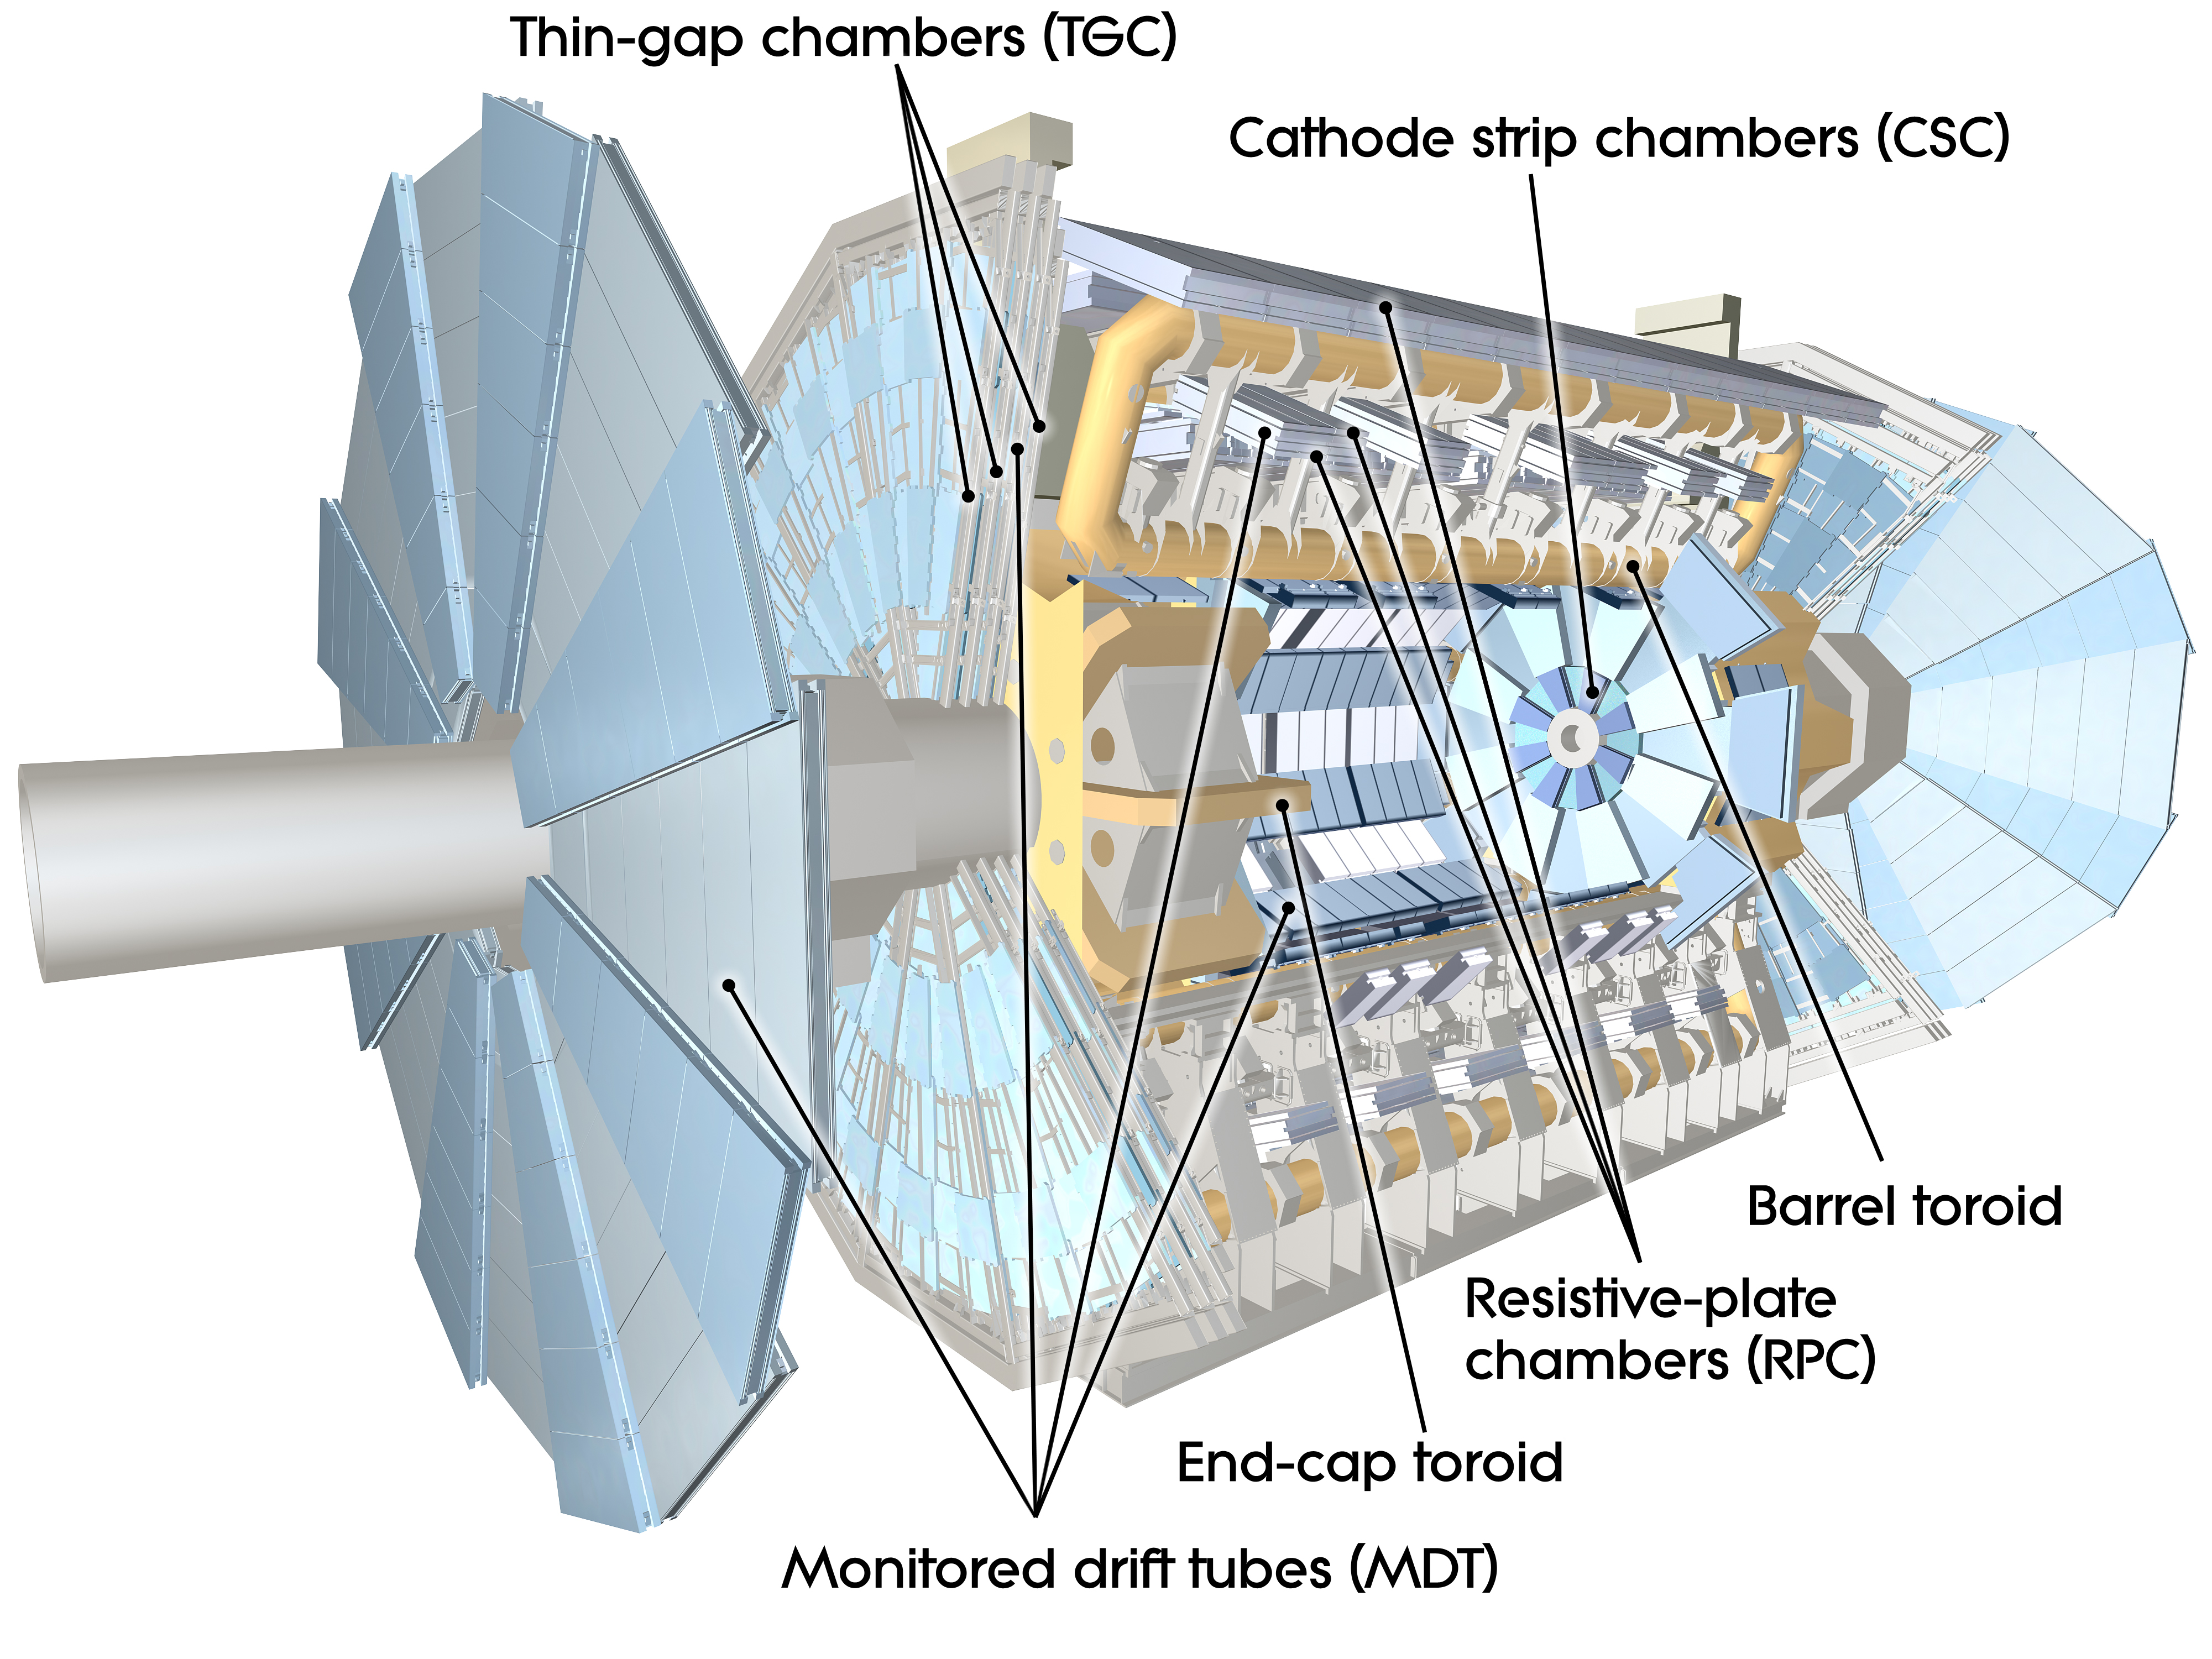
\includegraphics[width=\mediumfigwidth]{tex/experiment/ms_whole}
	\caption{Cut-away view of the ATLAS muon spectrometer \cite{ATLAS-detector}.}
	\label{fig:muon_spectrometer}
\end{figure}

The muon spectrometer (MS) provides precise tracking of muons that have exited the 
calorimeters. A huge air-core toroid magnet system generates a \unit{0.5}{\tesla} 
(\unit{1}{\tesla}) field in the barrel (end-caps), enabling momentum to be inferred from 
track curvature measurements. Four types of tracking chamber are installed in three 
layers (see \Figure~\ref{fig:muon_spectrometer}):
\begin{description}
\item[Monitored drift tubes (MDTs) and cathode strip chambers (CSCs)] \hfill \\
	MDTs and CSCs provide precise momentum measurement, with a resolution of 
	about \unit{40}{\micro\metre} in the bending plane. MDTs cover the region 
	$\mods{\eta} < 2.7$, but the innermost end-cap is replaced with CSCs to 
	withstand the higher particle flux. CSCs are multiwire proportional chambers 
	with cathode planes segmented into strips in orthogonal directions.
\item[Resistive plate chambers (RPCs) and thin gap chambers (TGCs)] \hfill \\
	RPCs and TGCs provide less precise tracking, but at a faster readout speed needed for 
	triggering. They also provide orthogonal coordinates to those of the MDTs and CSCs. 
	RPCs are gas-filled parallel plate detectors operated in avalanche mode.
	TGCs are multiwire proportional chambers operated in quasi-saturated mode.
\end{description}



\subsection{Trigger and data acquisition}
\label{sec:atlas:trig}

It is technically infeasible to record the detector readout (\unit{1.6}{\mega\bel} per 
event) at the bunch crossing rate expected at the LHC (\unit{40}{\mega\hertz}).
Moreover, the majority of these events are uninteresting in terms of the LHC physics 
program. For these reasons, ATLAS has a trigger system to identify and retain interesting
events for further analysis offline.

The trigger is split into three levels with successively lower event rates: level~1 (L1), 
level~2 (L2) and the event filter (EF). This is achieved by affording a longer latency 
for later levels to apply more refined selection criteria, as shown in 
\Figure~\ref{fig:trigger}. The L2 and EF triggers are collectively referred to as the 
high level trigger (HLT), and are implemented on an off-detector computer farm.

\begin{figure}[t]
	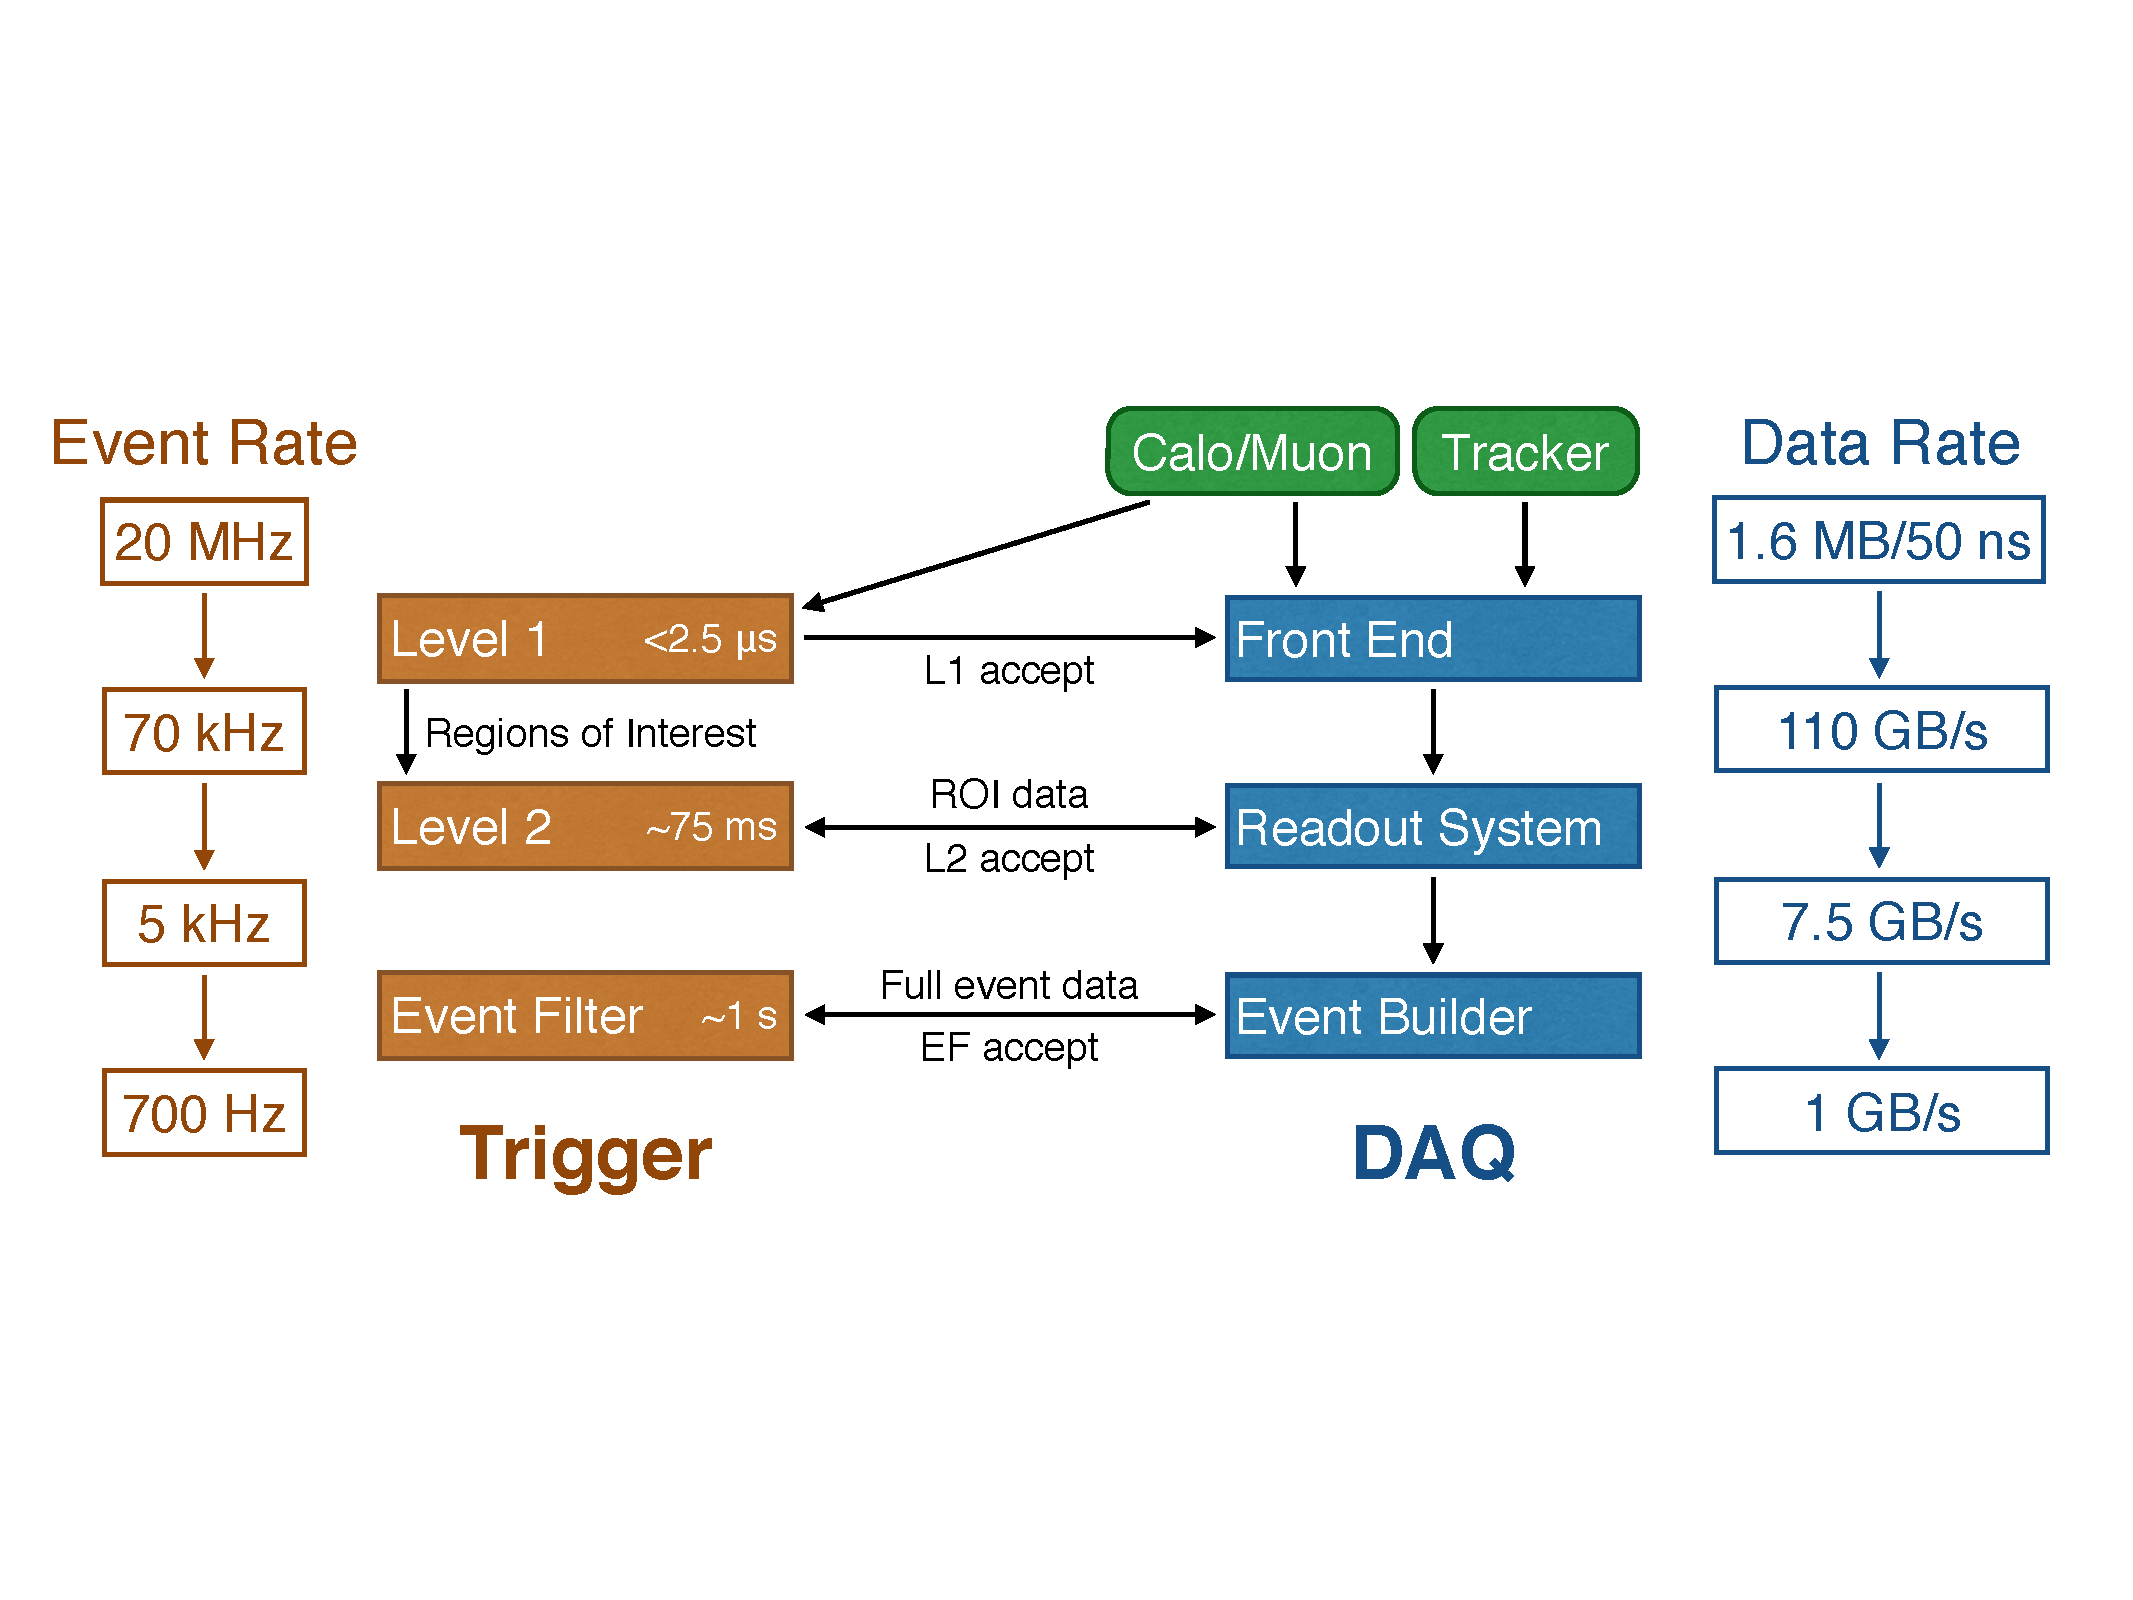
\includegraphics[width=\textwidth,clip=true,trim=0.9cm 6.8cm 1.4cm 6.8cm]{custom_images/trigger}
	\caption{Schematic diagram of the ATLAS trigger and data acquisition (DAQ) system.
	Typical values for event rates, data rates and trigger latencies during the 2012 run 
	are taken from \cite{TriggerNumbers}.}
	\label{fig:trigger}
\end{figure}

The L1 trigger searches for high-\pt leptons, photons and jets, in addition to 
events with significant total transverse energy or transverse energy imbalance. The 
decision is made using muon trigger chamber information (RPCs and TGCs) and 
reduced-granularity calorimeter information. Since the decision latency 
(\unit{2.5}{\micro\second}) is longer than the bunch spacing (\unit{25}{\nano\second}),
event data is stored in pipelines while a decision is made.

The detector coordinates of interesting features identified by the L1 trigger, known 
as regions of interest (ROIs), are passed on to the L2 trigger. The L2 trigger 
then requests the full degree of detector information for these ROIs (\about 2\% of total
event data), in order to make a more informed decision. Finally, the EF trigger has
access to the full event data, and further reduces the data rate such that it can be 
written to tape. The entire trigger system reduces the data rate from 
\unit{64}{\tera\bel\per\second} to about \unit{1}{\giga\bel\per\second}.



\subsection{Performance goals}

The performance goals of each sub-detector are shown in \Table~\ref{tab:atlas_targets}. 
The $\sigma_{\pt}/\pt$ of the tracker has a term proportional to \pt due to the 
intrinsic spatial resolution of the detector, and a constant term due to multiple 
scattering. The $\sigma_{E}/E$ of the calorimeters has a constant term due to 
non-uniformities in the response, and a term proportional to $1/\sqrt{E}$ due to 
statistical fluctuations in the hadronic shower (the \textit{stochastic term}). 

\begin{table}[h]
	\begin{tabular}{lr@{\;{=}\;}lcc}
		\toprule
		\multirow{2}{*}{Detector component} & 
		\multicolumn{2}{c}{\multirow{2}{*}{Required resolution}} & 
		\multicolumn{2}{c}{$\mods{\eta}$ coverage} \\
		& \multicolumn{2}{c}{} & Measurement & L1 trigger \\
		\midrule
		Tracker                  & $\sigma_{\pt}/\pt$ & $0.05\% \times \pt \oplus 1\%$ &
		$<2.5$ & -- \\
		EM calorimeter           & $\sigma_{E}/E$ & $10\% / \sqrt{E} \oplus 0.7\%$ &
		$<3.2$ & $<2.5$ \\
		Hadronic calorimeter     & \multicolumn{2}{l}{} & & \\
		\quad barrel and end-cap & $\sigma_{E}/E$ & $50\% / \sqrt{E} \oplus 3\%$ &
		$<3.2$ & $<3.2$ \\
		\quad   forward          & $\sigma_{E}/E$ & $100\% / \sqrt{E} \oplus 10\%$ &
		$3.1\text{ -- }4.9$ & $3.1\text{ -- }4.9$ \\
		Muon spectrometer        & $\sigma_{\pt}/\pt$ & $10\%$ at $\pt=\unit{1}{\TeV}$ &
		$<2.7$ & $<2.4$ \\
		\bottomrule
	\end{tabular}
	\caption{Performance goals of the ATLAS sub-detectors \cite{ATLAS-detector}. Energies 
	and momenta are given in \GeV. The quoted MS performance is independent of the 
	ID. The contribution of electronic noise to $\sigma_{E}/E$ is neglected (a term 
	proportional to $1/E$).}
	\label{tab:atlas_targets}
\end{table}

  
  \chapter{Overview of the \HWW analysis}
    \label{chap:selection}
    %!TEX root = ../../thesis.tex

The \WW decay of the Higgs boson is a promising search channel as it has a large \ac{BR} 
for a wide range of \mH. In fact, it is the most probable decay for 
\unit{$\mH > 135$}{\GeV} (see \Figure~\ref{fig:higgs_br}). This chapter will describe the 
experimental search for \ggHWWlvlv (where $\Plepton = \Pe, \Pmu$) using the 2012 dataset 
of \pp collisions at \unit{$\sqrt{s} = 8$}{\TeV}. The search strategy is optimised for a 
low mass Higgs boson, as favoured by electroweak fits, and thus accounts for off-shell \PW 
bosons.

The experimental signature of this search involves electrons, muons, jets and transverse 
momentum imbalance, and is 
outlined in \Section~\ref{sec:signature}. Then, \Section~\ref{sec:objects} details how 
each of these objects is reconstructed by the ATLAS detector. Finally, 
\Section~\ref{sec:selection} describes the criteria by which Higgs boson events are 
selected and background events are rejected. In doing so, it is necessary to make 
reference to many exclusive observables of signal and background processes. However, 
the modelling and estimation of these observables shall be described later, in 
Chapters~\ref{chap:signal}, \ref{chap:ww} and \ref{chap:backgrounds}.

    \section{Experimental signature}
      \label{sec:signature}
      %!TEX root = ../../thesis.tex

Following the \HWW decay, each \PW boson will decay leptonically or hadronically, with 
$\text{BR}\parenths{\HepProcess{\PW\HepTo\Plepton\Pnu}} = 10.8\%$ and 
$\text{BR}\parenths{\HepProcess{\PW\HepTo \text{hadrons}}} = 67.6\%$ \cite{PDG:2012}. 
Thus, \textit{dileptonic}, \textit{semi-leptonic} and \textit{hadronic} final states are 
conceivable. Although the dileptonic channel is suppressed by \acp{BR}, it is ultimately 
the most sensitive as the other two have larger experimental backgrounds. This chapter 
will describe the dileptonic search, and henceforth 
`lepton' and \Plepton shall refer to an electron or muon.\footnote{
	Events with one or two \HepProcess{\PW\HepTo\Ptau\Pnu} decays can 
	contribute to the dileptonic search when the \Ptau decays to an electron or muon. This 
	contribution is small however, since
	$\text{BR}\parenths{\HepProcess{\Ptau\HepTo\Plepton\Pnulepton\Pnut}} = 17.6\%$ 
	\cite{PDG:2012}. Also, the kinematics of such events are different due to the 
	additional decay(s) and neutrinos.
}

Electroweak fits favour a Higgs boson with mass $\mH < 2\mW$ (see \Figure~\ref{fig:ewfit}).
It is therefore important for the \HWW search to be sensitive to off-shell \PW bosons. 
Experimentally, this means using leptons with lower \pt thresholds, which unfortunately 
are more susceptible to fakes.

Since neutrinos do not interact with the detector, it is only possible to infer their 
transverse momentum from an imbalance in the visible momenta, called \met. When there are 
multiple neutrinos, only the transverse component of the vector sum of the neutrino 
momenta can be inferred from the \met. Thus, it is not possible to fully reconstruct a 
mass peak in the \HWWlvlv search, and to be sensitive to the Higgs boson it becomes 
crucial to understand the many background processes.

The basic experimental signature is two oppositely charged leptons and significant \met. 
However, there are background processes that exhibit the same signature. Others have an 
aspect of the signature faked by mismeasurement, or some part of their final state fails 
reconstruction. \Table~\ref{tab:bkg_summary} introduces the different backgrounds. Jets 
are a convenient way to separate the contributions of different background processes.

Jets can also be used to separate the \ac{ggF} and \ac{VBF} production modes of the Higgs 
boson (see \Section~\ref{sec:properties}). The search described below is designed for the 
\ac{ggF} production mode though, and this shall become particularly apparent when 
describing the \twojet bin in \Section~\ref{sec:selection:2j}.

\begin{table}
	\begin{tabular}{l@{\hskip 0.3in}l}
		\toprule
		Background        & Mechanism of \HepProcess{\Plepton\Plepton + \met} signature \\
		\midrule
		\WW               & irreducible \\
		\ttbar, \HepProcess{\PW \Ptop} & irreducible (aided by jet \Pbottom-tagging) \\
		other single top  & jet fakes lepton \\
		\DYll             & fake \met \\
		\DYtt             & irreducible \\
		\Wjets, dijet     & jet(s) fake lepton(s) \\
		\Wgamma           & photon fakes electron \\
		\WZ, \Wgstar, \ZZ & lepton(s) fail selection \\
		\bottomrule
	\end{tabular}
	\caption{Summary of how each background produces the 
	\HepProcess{\Plepton\Plepton + \met} experimental signature.}
	\label{tab:bkg_summary}
\end{table}

    \section{Reconstruction of physics objects}
      \label{sec:objects}
      %!TEX root = ../../thesis.tex

\subsection{Electrons}
\subsection{Muons}
\subsection{Jets}
\subsection{Missing transverse momentum}

    \section{Event selection criteria}
      \label{sec:selection}
      %!TEX root = ../../thesis.tex

\Section~\ref{sec:signature} outlined the basic experimental signature of the search as 
two oppositely charged leptons and significant \met. Thus, the initial stages of the 
event selection are responsible for finding this signature. Subsequent criteria, or 
\textit{cuts}, target specific background processes. Their aim is to improve the analysis 
sensitivity by suppressing backgrounds whilst retaining a sufficient number of signal events.



\subsection{Data quality}
\label{sec:selection:quality}

The \pp dataset (see \Section~\ref{sec:dataset:dataset}) is hierarchically split into 
\textit{periods} of broadly consistent beam conditions, \textit{runs} typically 
corresponding to LHC fills, and \textit{luminosity blocks} of \about 2~minutes where the 
instantaneous luminosity is approximately constant. Luminosity blocks are included in the 
analysis if the detector was operating sufficiently for the recorded data to be 
considered `good for physics' (see \Figure~\ref{fig:dataset:lumi}).\footnote{
	ATLAS good runs list: \texttt{data12\symbol{95}8TeV.periodAllYear\symbol{95}DetStatus-v61-pro14-02\symbol{95}DQDefects-00-01
	-00\symbol{95}PHYS\symbol{95}StandardGRL\symbol{95}All\symbol{95}Good.xml}
} 
For the 2012 dataset, this corresponds to a total integrated luminosity of 
\unit{20.3}{\invfb}.

Individual events are also vetoed if certain data quality criteria are failed by:
\begin{itemize}[noitemsep,nolistsep]
	\item a noise burst in the LAr calorimeter,
	\item data corruption caused by a restart of the synchronisation system,
	\item a \textit{looser} jet is reconstructed with \unit{$\pt > 20$}{\GeV} (indicative 
	of an HCal spike),
	\item a jet is reconstructed near a `hot' HCal tile (1st -- 8th May 2012 only).
\end{itemize}
A further quality criterion requires that the primary vertex considered as the hard 
scatter (that with the highest $\sum p_{\text{T}}^2$) must be associated with at least 
three tracks. This reduces the cosmic ray background to negligible levels.



\subsection{Trigger}
\label{sec:selection:trigger}

It is infeasible to record all the delivered collisions; ATLAS employs a trigger system to 
identify and record interesting events (see \Section~\ref{sec:atlas:trig}). In the \HWWlvlv 
search it is natural to trigger on high-\pt leptons, using algorithms similar to, though less 
sophisticated than, those in \Section~\ref{sec:objects:electrons} and 
\Section~\ref{sec:objects:muons}.

A trigger is characterised by its efficiency versus \pt curve (though it also depends on 
$\eta$), which has a turn-on followed by a plateau, as shown in 
\Figure~\ref{fig:sel:trig_eff}. It is preferable to operate on the plateau, where the 
efficiency is more stable and has smaller uncertainty. To maximise the signal yield, it is 
desirable to use a trigger with a lower turn-on \pt. However, increased backgrounds and 
limitations to trigger latency and bandwidth require a compromise to be found. The lowest 
unprescaled\footnote{
	A \textit{prescaled} trigger reduces the turn-on \pt by recording only 1 in $N$ 
	events passing the trigger, and weighting such events by a factor $N$. In doing so, 
	some statistical power is lost.
}
single lepton triggers available in 2012 had nominal \pt thresholds of \unit{24}{\GeV}. 
Fortunately, it is possible to recover trigger efficiency at lower \pt by using dilepton 
triggers, because the backgrounds are much smaller.

\begin{figure}[t]
	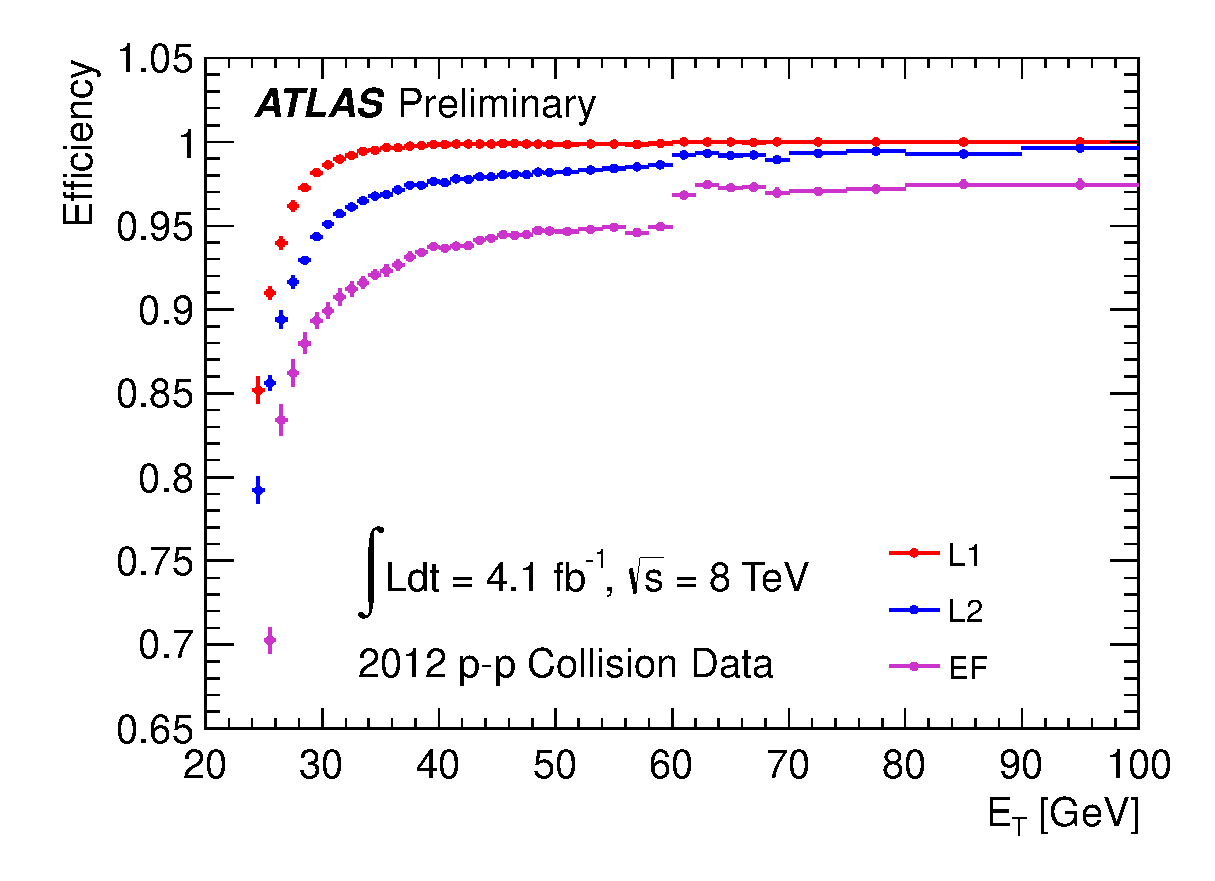
\includegraphics[width=0.495\textwidth]{tex/selection/trigger_eff_el}
	\hfill
	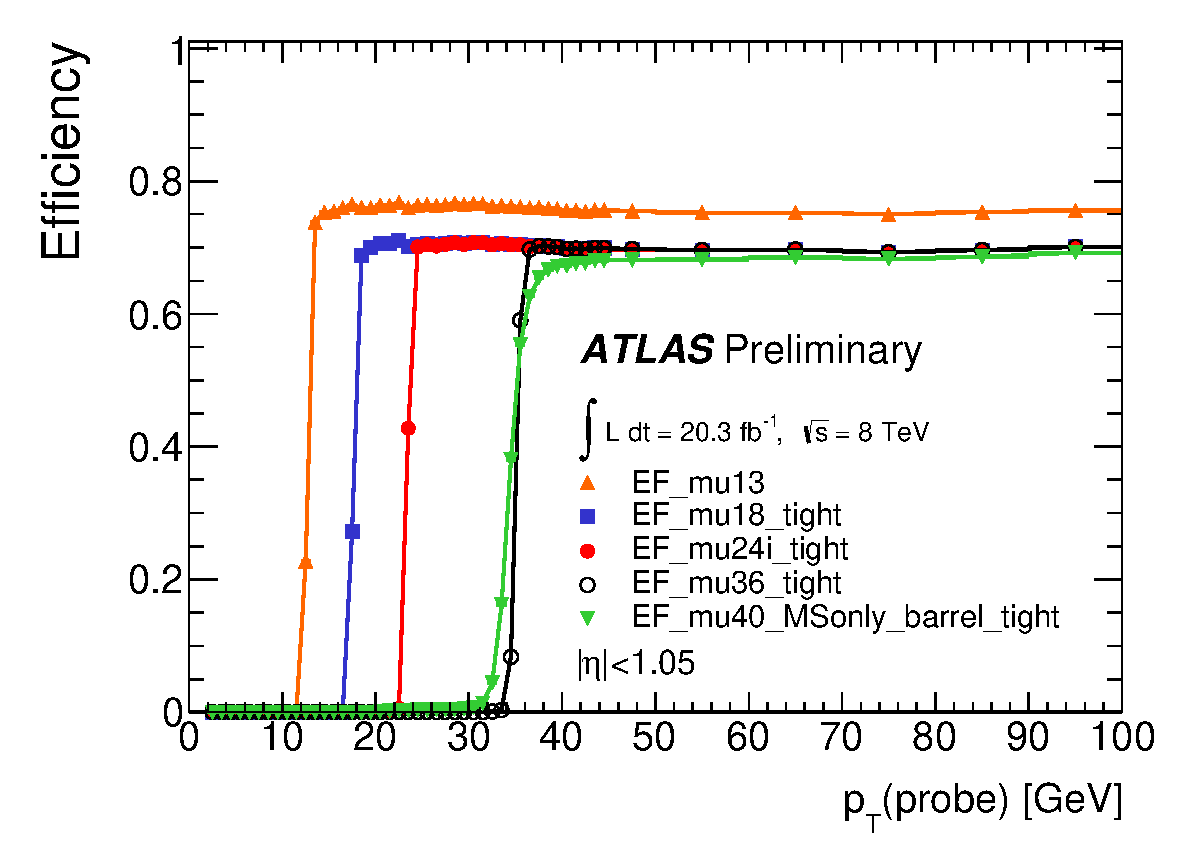
\includegraphics[width=0.495\textwidth]{tex/selection/trigger_eff_mu}
	\caption{Efficiencies of the single lepton triggers for electrons with respect to 
	offline \textit{medium} identification (left) and muons with respect to offline 
	reconstruction (right).}
	\label{fig:sel:trig_eff}
\end{figure}

\begin{table}[t]
	\begin{tabular}{lllcl}
		\toprule
		\multirow{2}{2.5cm}{Single lepton triggers} & \Pe  & \verb|EF_e24vhi_medium1| & or & \verb|EF_e60_medium1| \\
		& \Pmu & \verb|EF_mu24i_tight| & or & \verb|EF_mu36_tight|  \\
		\midrule
		\multirow{3}{2.5cm}{Dilepton triggers} & \HepProcess{\Pe\Pe} & \verb|EF_2e12Tvh_loose1| & or & \verb|EF_2e12Tvh_loose1_L2StarB| \\
		& \HepProcess{\Pmu\Pmu} & \multicolumn{3}{l}{\texttt{EF\symbol{95}mu18\symbol{95}tight\symbol{95}mu8\symbol{95}EFFS}} \\
		& \HepProcess{\Pe\Pmu}  & \multicolumn{3}{l}{\texttt{EF\symbol{95}e12Tvh\symbol{95}medium1\symbol{95}mu8}} \\
		\bottomrule
	\end{tabular}
	\caption{Employed triggers. \texttt{EF} refers to event filter, \texttt{e} is an 
	electron, \texttt{mu} is a muon, the following number is the \pt threshold, 
	\texttt{vh} indicates calorimeter isolation, \texttt{i} indicates track isolation, 
	and \texttt{tight}, \texttt{medium} or \texttt{loose} is the identification. Other 
	parts relate to the trigger chain. Criteria are looser than those applied 
	offline.}
	\label{tab:sel:triggers}
\end{table}

Events are required to pass at least one trigger listed in \Table~\ref{tab:sel:triggers}. 
The single lepton triggers include a tighter low-\pt trigger and a looser high-\pt 
trigger in order to maximise the efficiency. Dilepton triggers are then used to recover some 
efficiency at lower \pt. Together, these triggers support a \pt threshold of \unit{22}{\GeV} 
on the leading lepton (in the offline analysis), whilst operating on the plateau.

Additionally, events are required to have at least one lepton passing the offline 
reconstruction that is matched within $\Delta R < 0.15$ of a triggered lepton object.
Single lepton triggers are matched to offline leptons with $\pt > \unit{25}{\GeV}$. On 
the other hand, dilepton triggers comprise two triggered objects: \texttt{mu8} is matched 
to offline muons with $\pt > \unit{10}{\GeV}$, \texttt{mu18} is matched to offline muons 
with $\pt > \unit{20}{\GeV}$, and \texttt{e12} is matched to offline electrons with 
$\pt > \unit{15}{\GeV}$.\footnote{
	It follows that events featuring an electron with \unit{$\pt < 15$}{\GeV} must fire a 
	single lepton trigger, and thus the leading lepton must have \unit{$\pt > 25$}{\GeV}.
}

Lepton trigger efficiencies are measured via tag-and-probe of 
\HepProcess{\PZ \HepTo \Plepton\Plepton} events, where the tag and probe have both 
passed the offline lepton selection and the tag has successfully matched to a triggered 
lepton object. For example, single lepton trigger efficiencies are displayed in 
\Figure~\ref{fig:sel:trig_eff}. Comparison with MC yields efficiency scale factors.



\subsection{Pre-selection of dilepton + \met signature}
\label{sec:selection:presel}

Following the trigger selection, events are required to have two oppositely charged 
leptons passing the offline selection (see \Section~\ref{sec:objects}). The lepton with 
the highest \pt, called the \textit{leading lepton}, must have 
\unit{$\ptleadlep > 22$}{\GeV} in order to operate on the trigger plateau. The 
\textit{subleading lepton} must have \unit{$\ptsubleadlep > 10$}{\GeV}, as specified in 
\Section~\ref{sec:objects}. Events containing a third lepton are vetoed in order to 
reject backgrounds with three or more leptons in the final state, such as \WZ production.

At this point, it is possible to split the dilepton final state into four channels 
according to the flavours of the two leptons: \eech, \mmch, \emch, \mech (where the first 
flavour is that of the leading lepton). This is very useful because the background 
compositions of the channels are dramatically different. For example, the \DYll background 
is much larger in the same flavour channels (\eech/\mmch) than the different flavour 
channels (\emch/\mech).

Low mass hadronic resonances with dileptonic decays (\eg \PJpsi) are removed from the 
\eech/\mmch channels by requiring the mass of the dilepton system \unit{$\mll > 12$}{\GeV}. 
This also greatly suppresses the low mass \DY background. For the \emch/\mech channels, 
a cut of \unit{$\mll > 10$}{\GeV} suppresses leptons from heavy flavour decays. The 
\eech/\mmch channels are hugely dominated by the \DY background (see 
\Figure~\ref{fig:sel:mll}), but most of these events can be rejected by 
vetoing a window around the \PZ mass, \unit{$\mods{\mll - \mZ} > 15$}{\GeV}.

\begin{figure}
	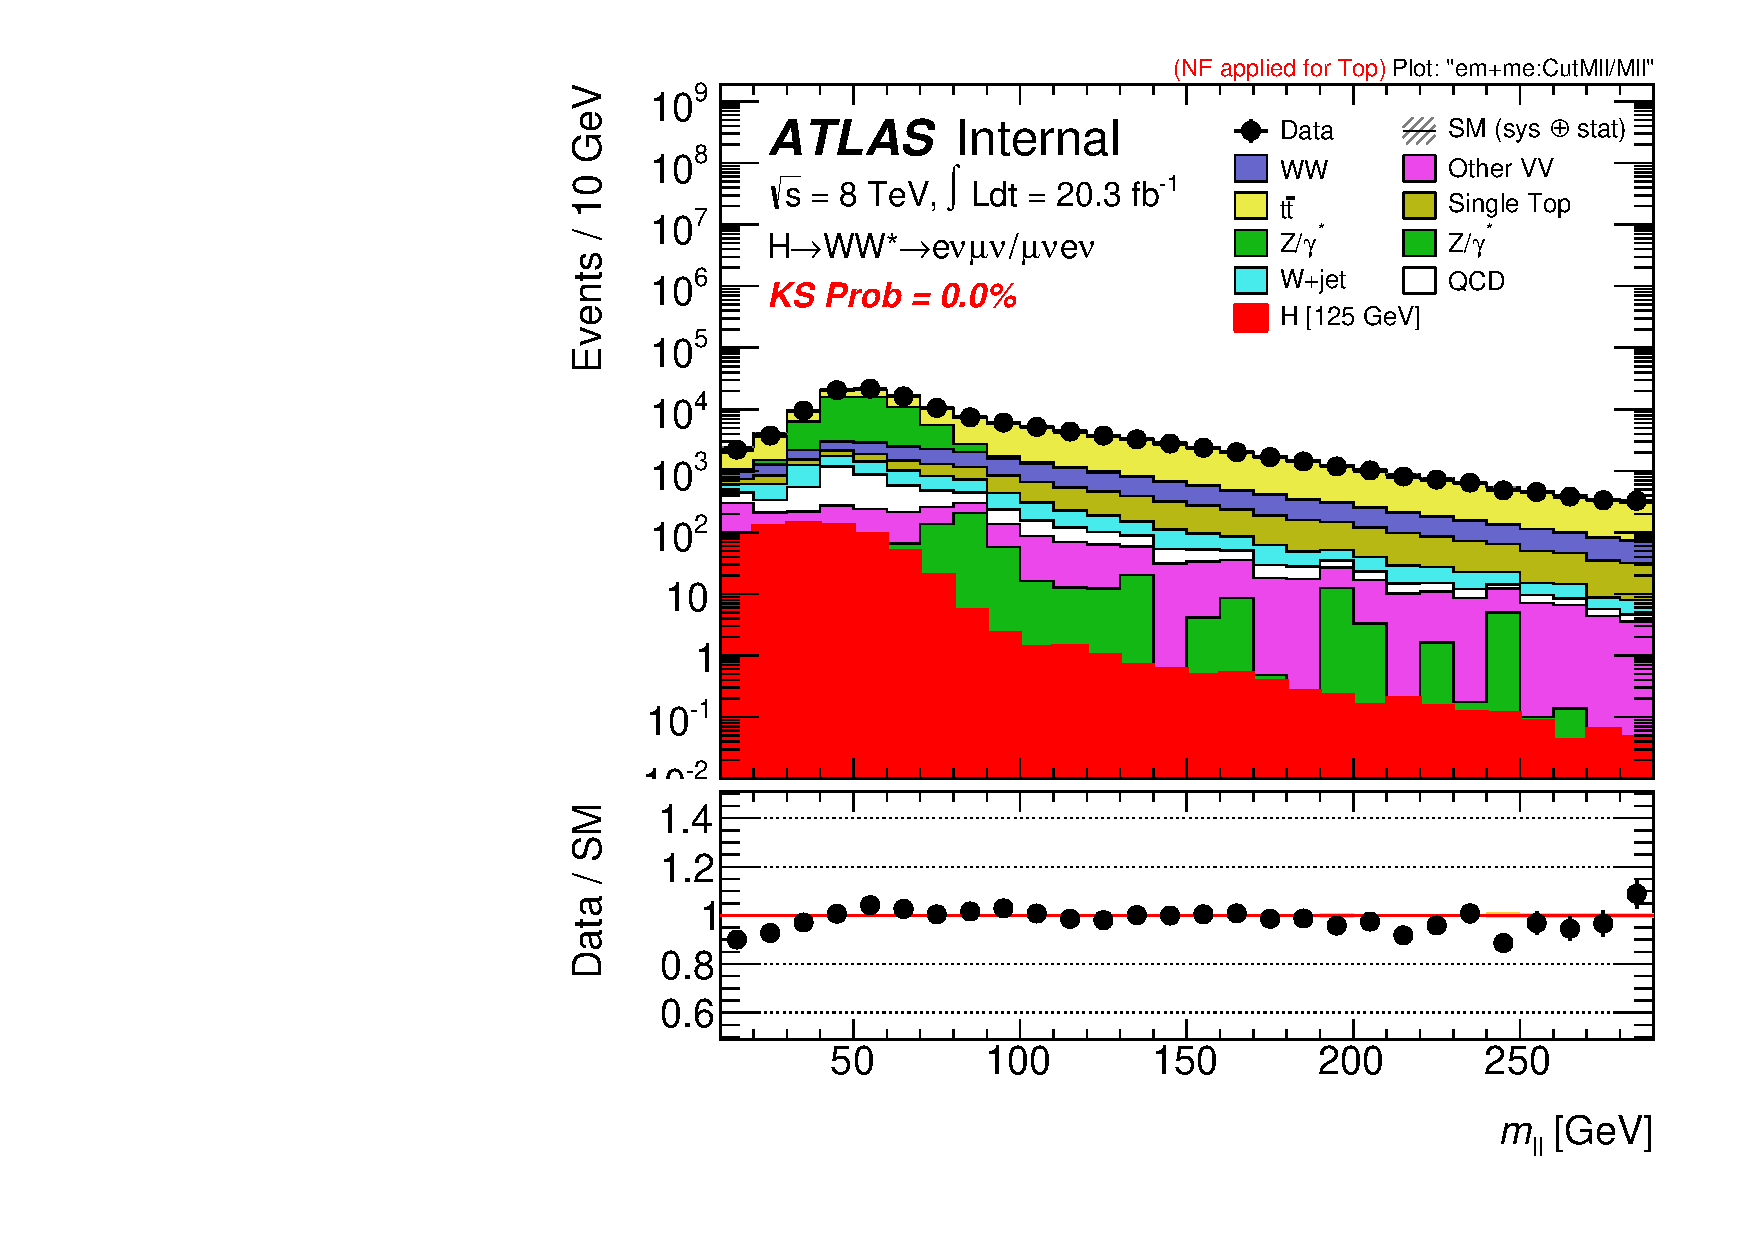
\includegraphics[width=0.495\textwidth]{tex/selection/emme_CutMll_Mll_mh125_log}
	\hfill
	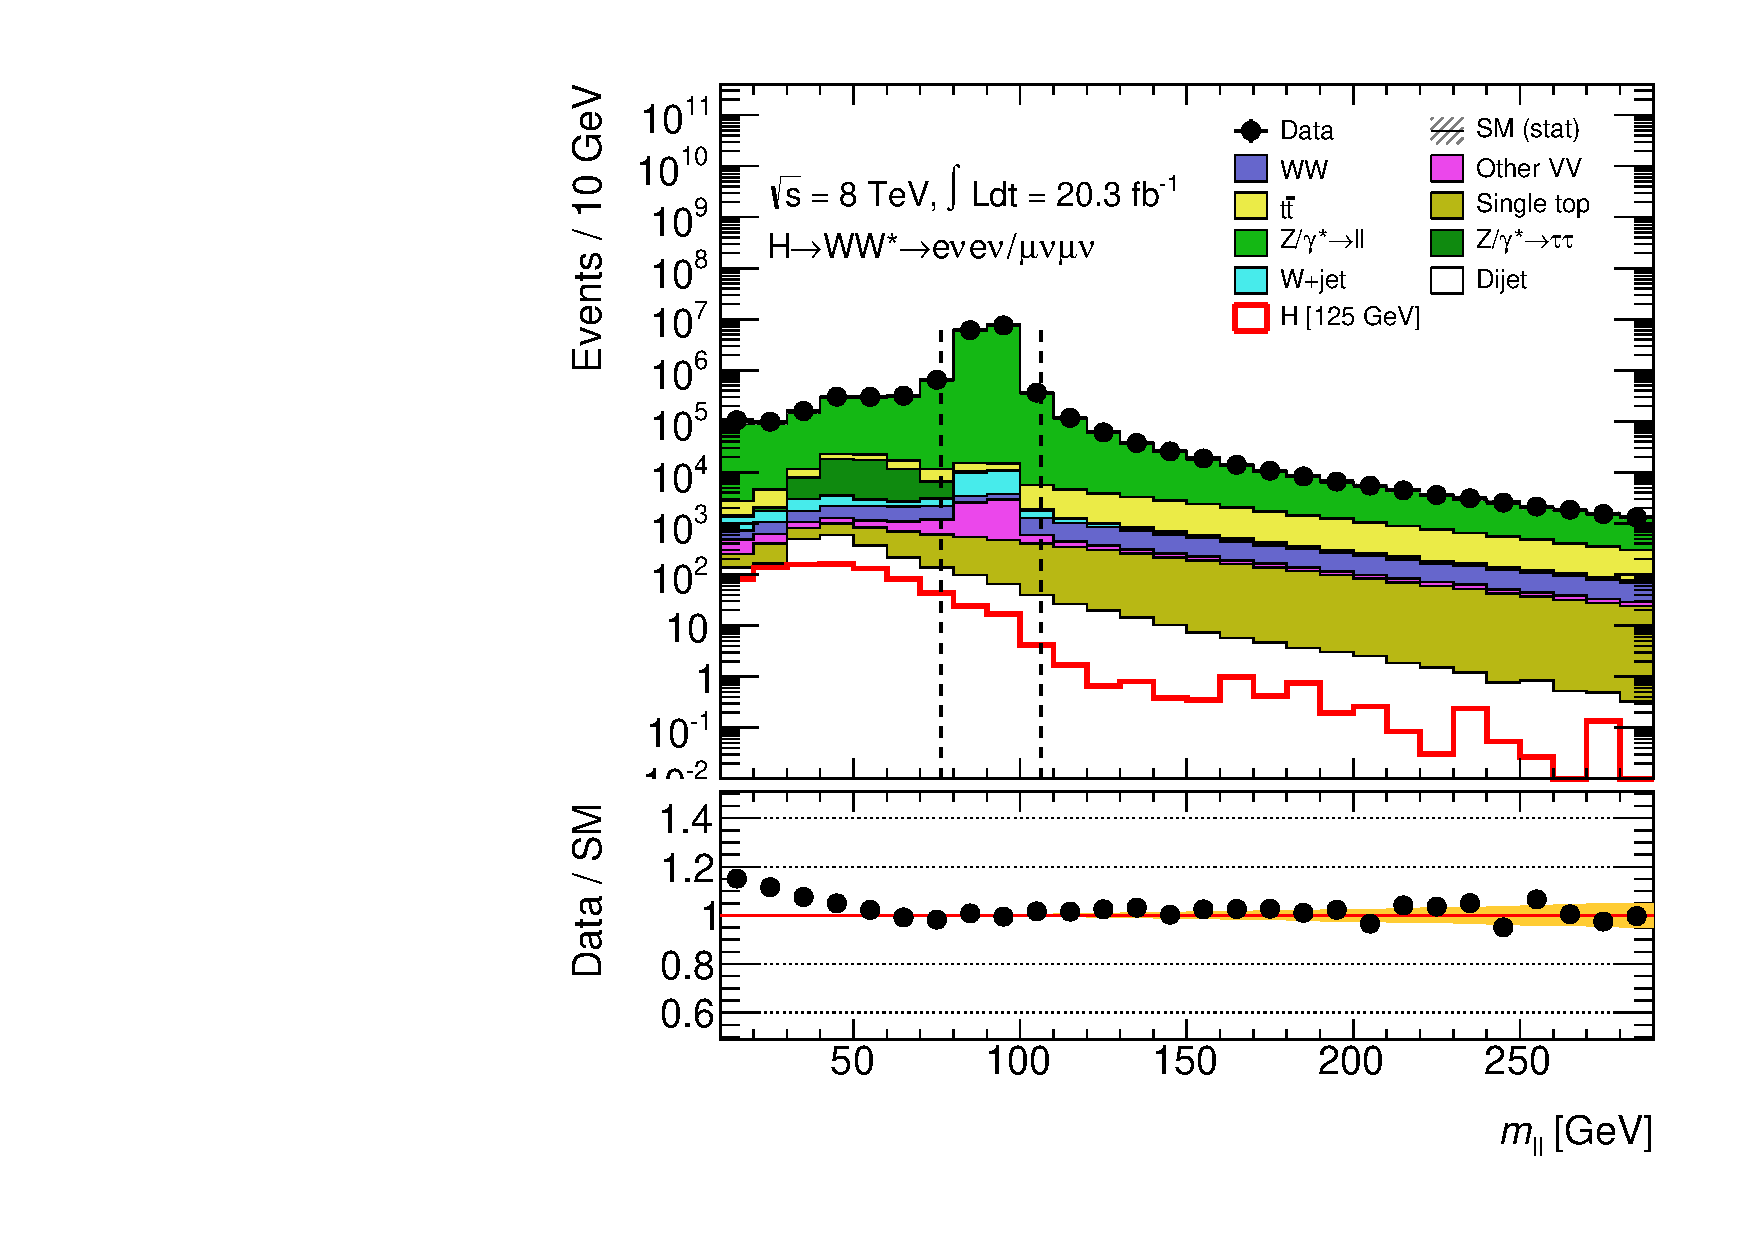
\includegraphics[width=0.495\textwidth]{tex/selection/eemm_CutMll_Mll_mh125_log}
	\caption{The \mll distribution in the \emch/\mech (left) and \eech/\mmch (right) 
	channels. These are made after the low \mll cut.}
	\label{fig:sel:mll}
\end{figure}

\begin{figure}
	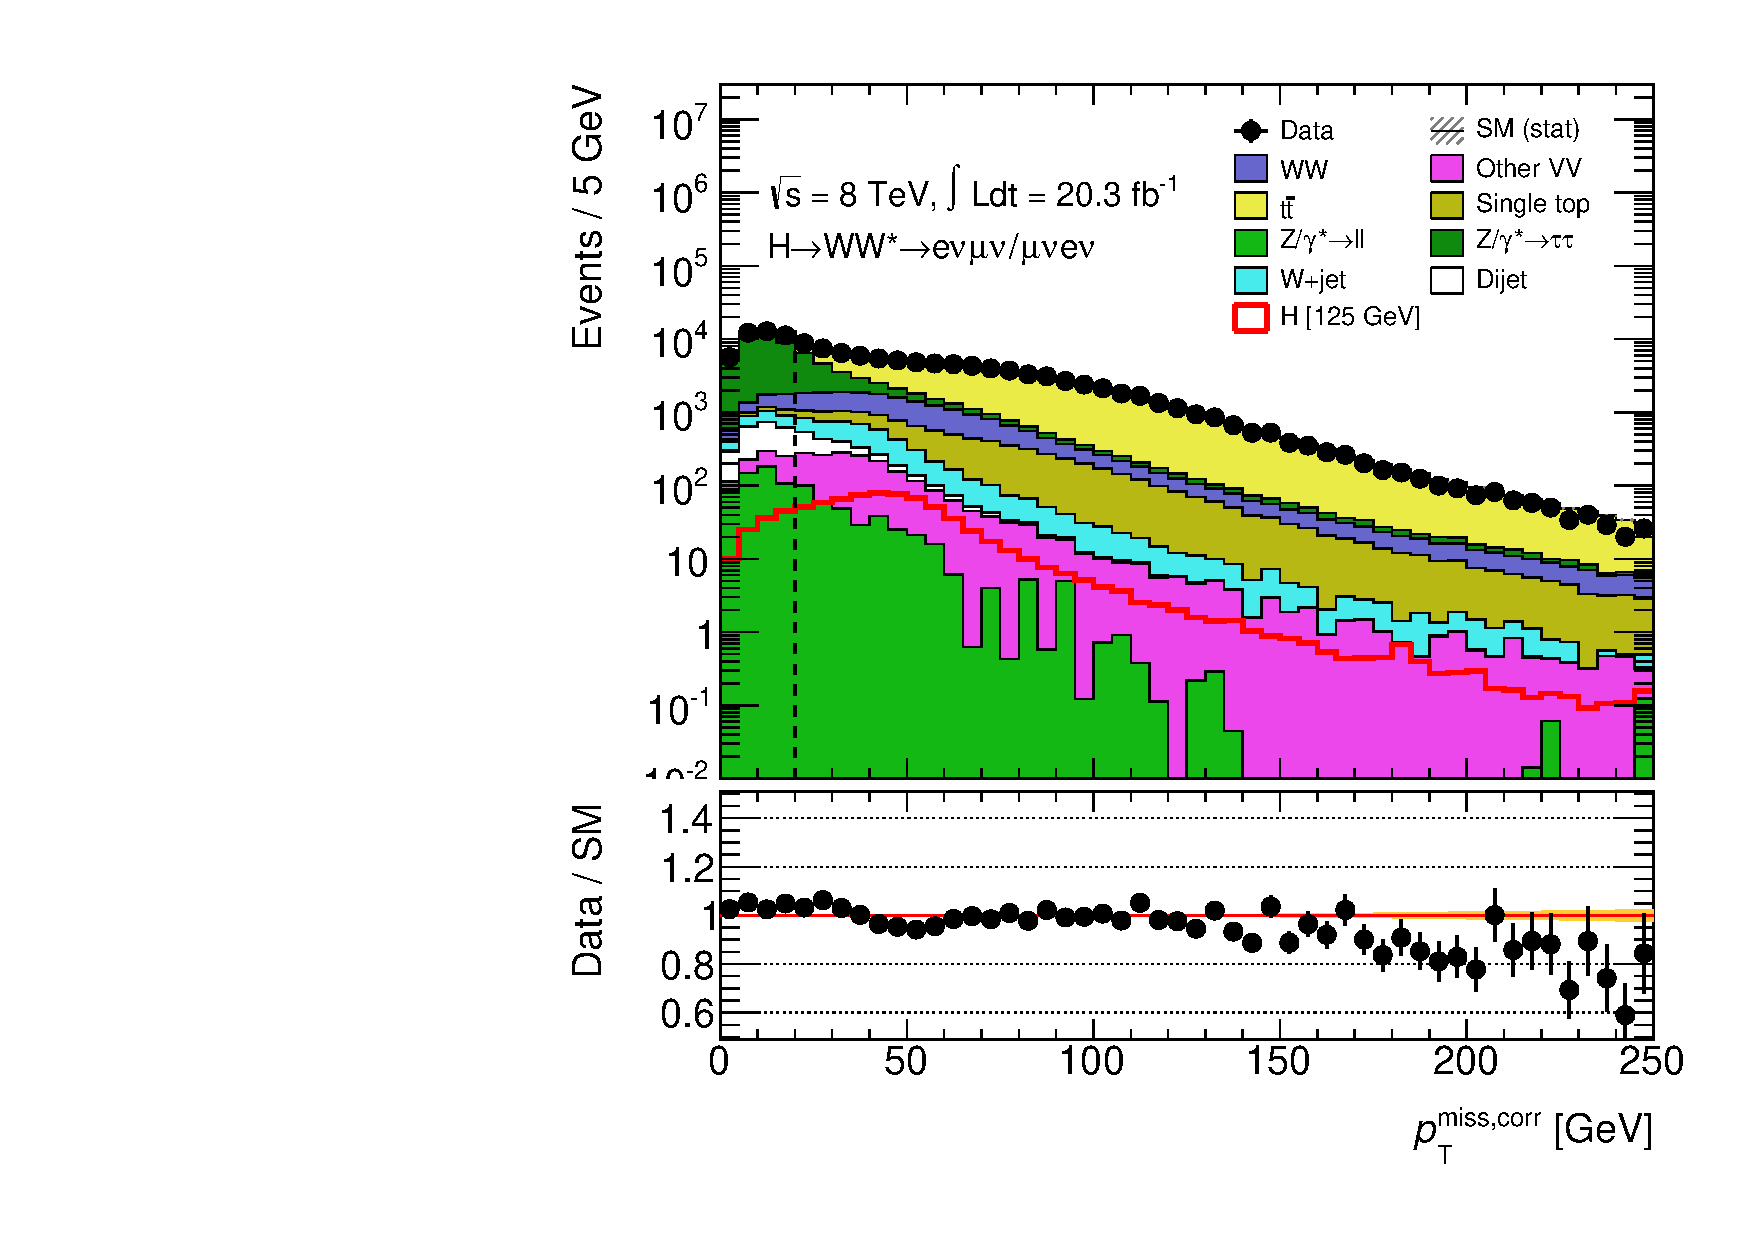
\includegraphics[width=0.495\textwidth]{tex/selection/emme_CutZVeto_MET_TrackHWW_Clj_mh125_log}
	\hfill
	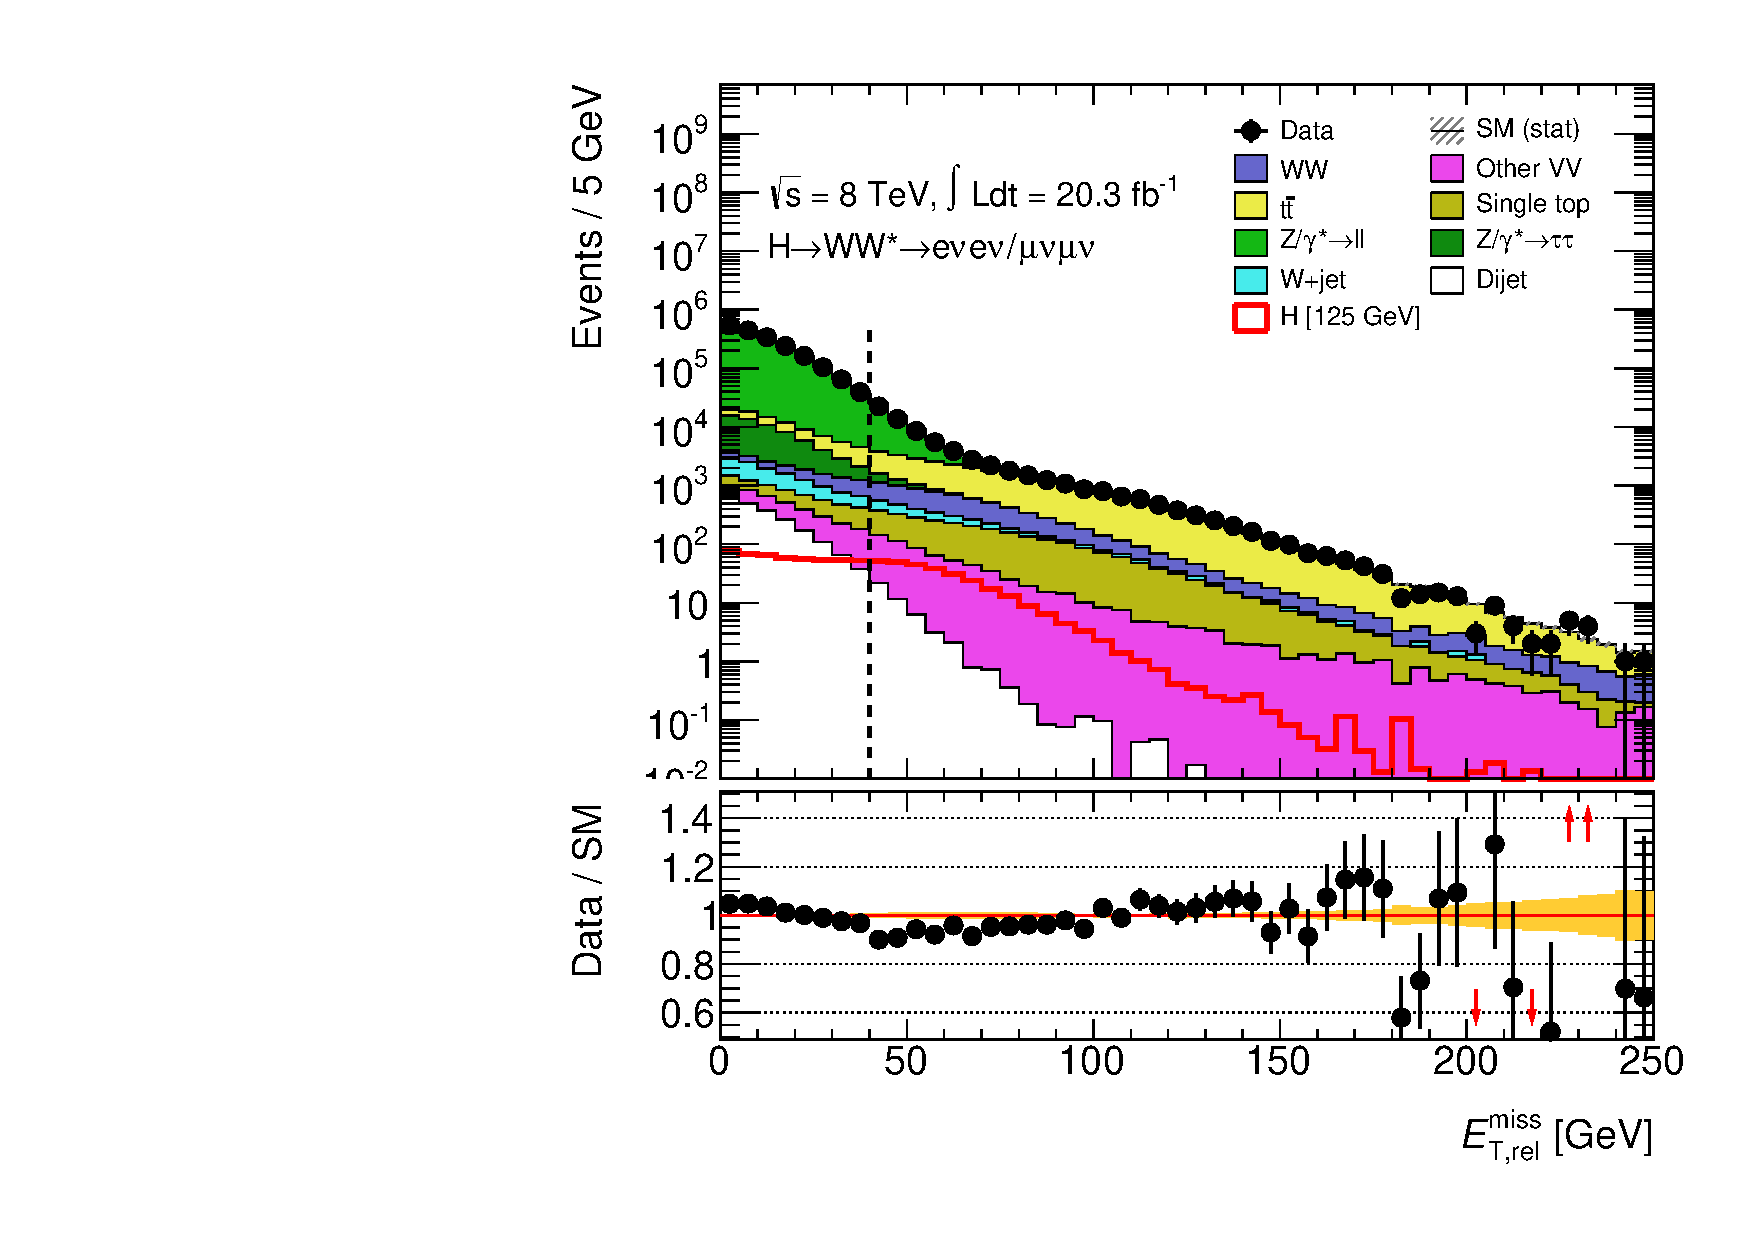
\includegraphics[width=0.495\textwidth]{tex/selection/eemm_CutZVeto_METRel_mh125_log}
	\caption{The \met variable cut upon in the \emch/\mech (left) and \eech/\mmch (right) 
	channels. These are made after the \PZ mass veto cut.}
	\label{fig:sel:met}
\end{figure}

Requiring significant \met suppresses the \DYll and dijet backgrounds (see 
\Figure~\ref{fig:sel:met}). It also suppresses the \DYtt background as its neutrinos have a 
propensity to cancel in the \met calculation. We require \unit{$\corrtrackmet > 20$}{\GeV} 
in the \emch/\mech channels and \unit{$\metrel > 40$}{\GeV} in the \eech/\mmch channels. In 
the \emch/\mech channels, the \met cut is relaxed because the \DYll background is smaller. 

Following the selection of dilepton events with significant \met, the \emch/\mech 
channels are dominated by top background and the \eech/\mmch channels are dominated by 
\DYll. However, the background compositions of all channels are highly dependent upon the 
number of jets (see \Figure~\ref{fig:sel:njets}). Thus, at this stage the analysis is 
binned according to jet multiplicity (0-jet, 1-jet, \twojet), so that backgrounds can be 
targeted individually. In the \twojet bin, only the \emch/\mech channels are used.

\begin{figure}[t]
	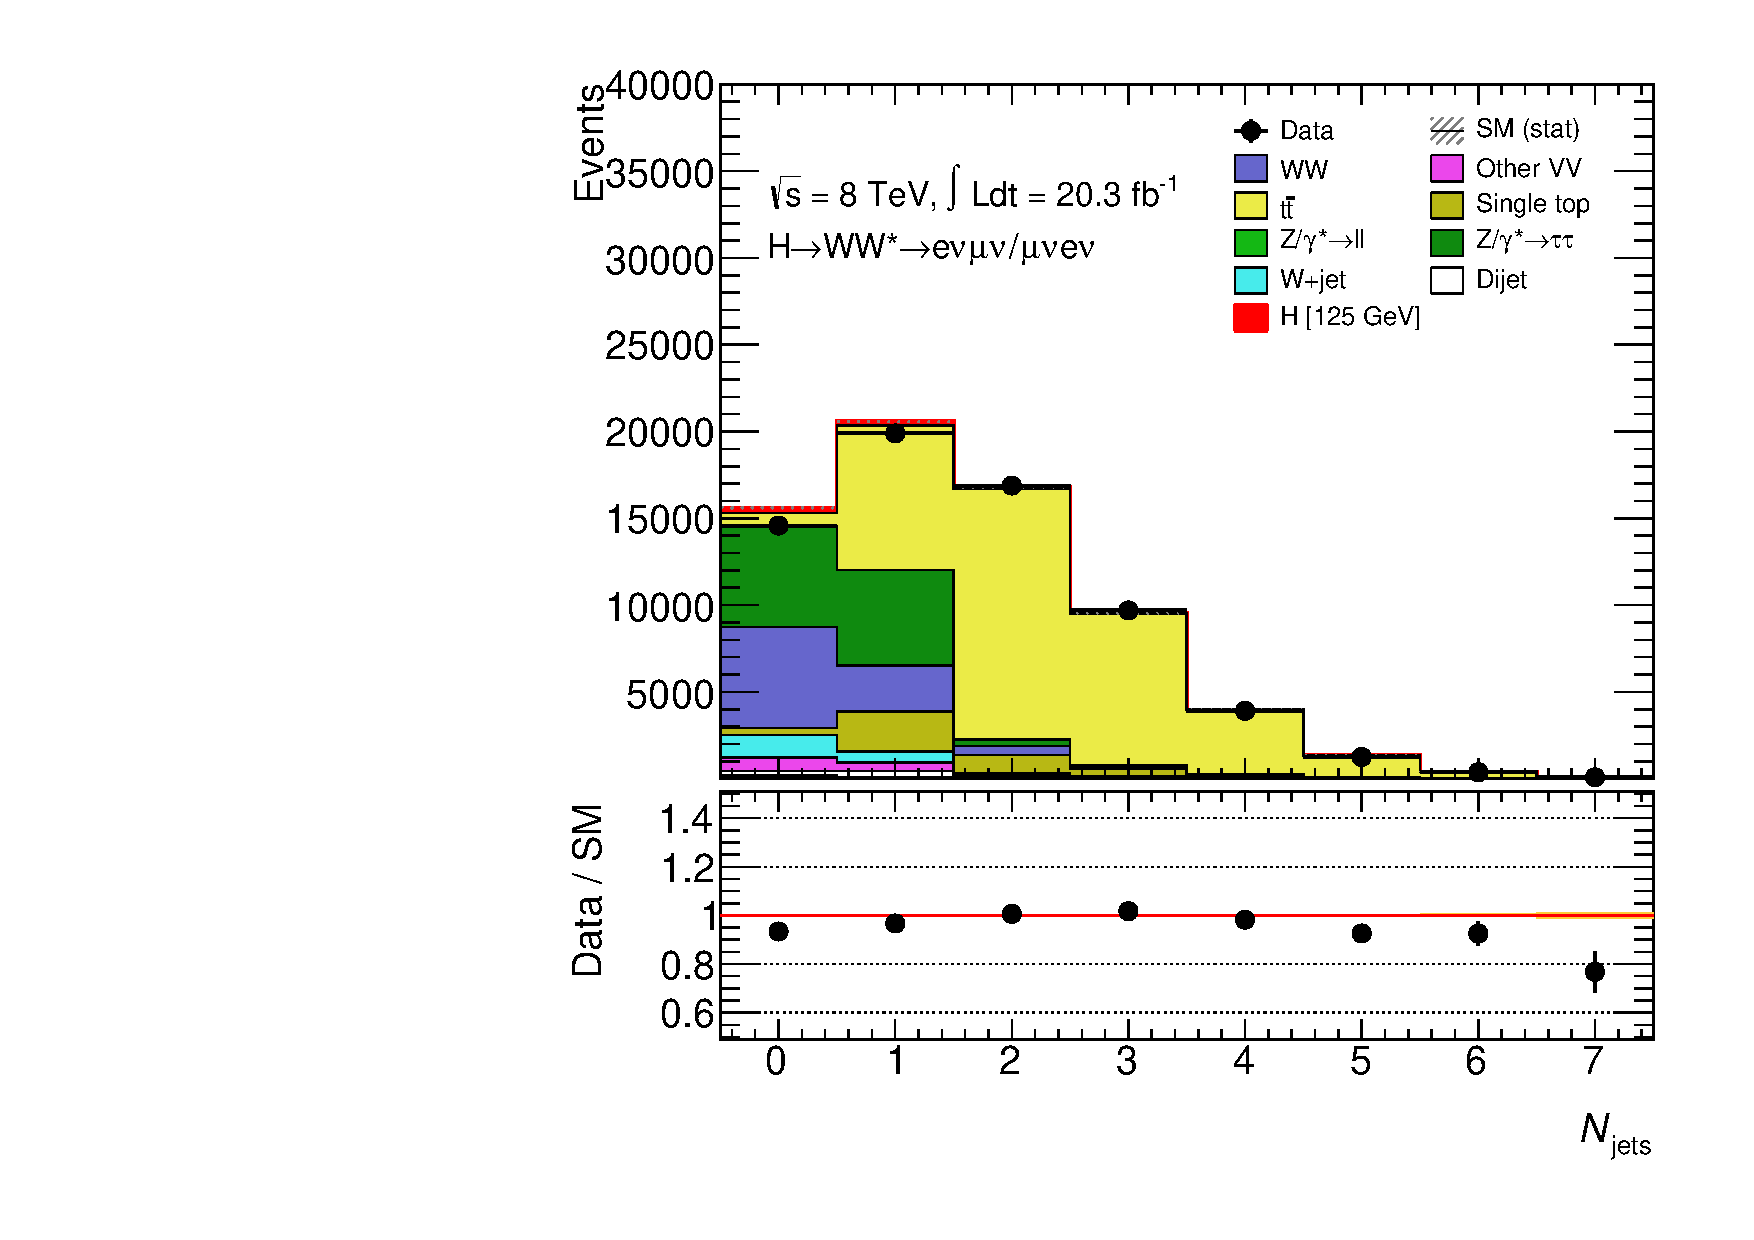
\includegraphics[width=0.495\textwidth]{tex/selection/emme_CutMETRel_m_jet_n_upTo7_mh125_lin}
	\hfill
	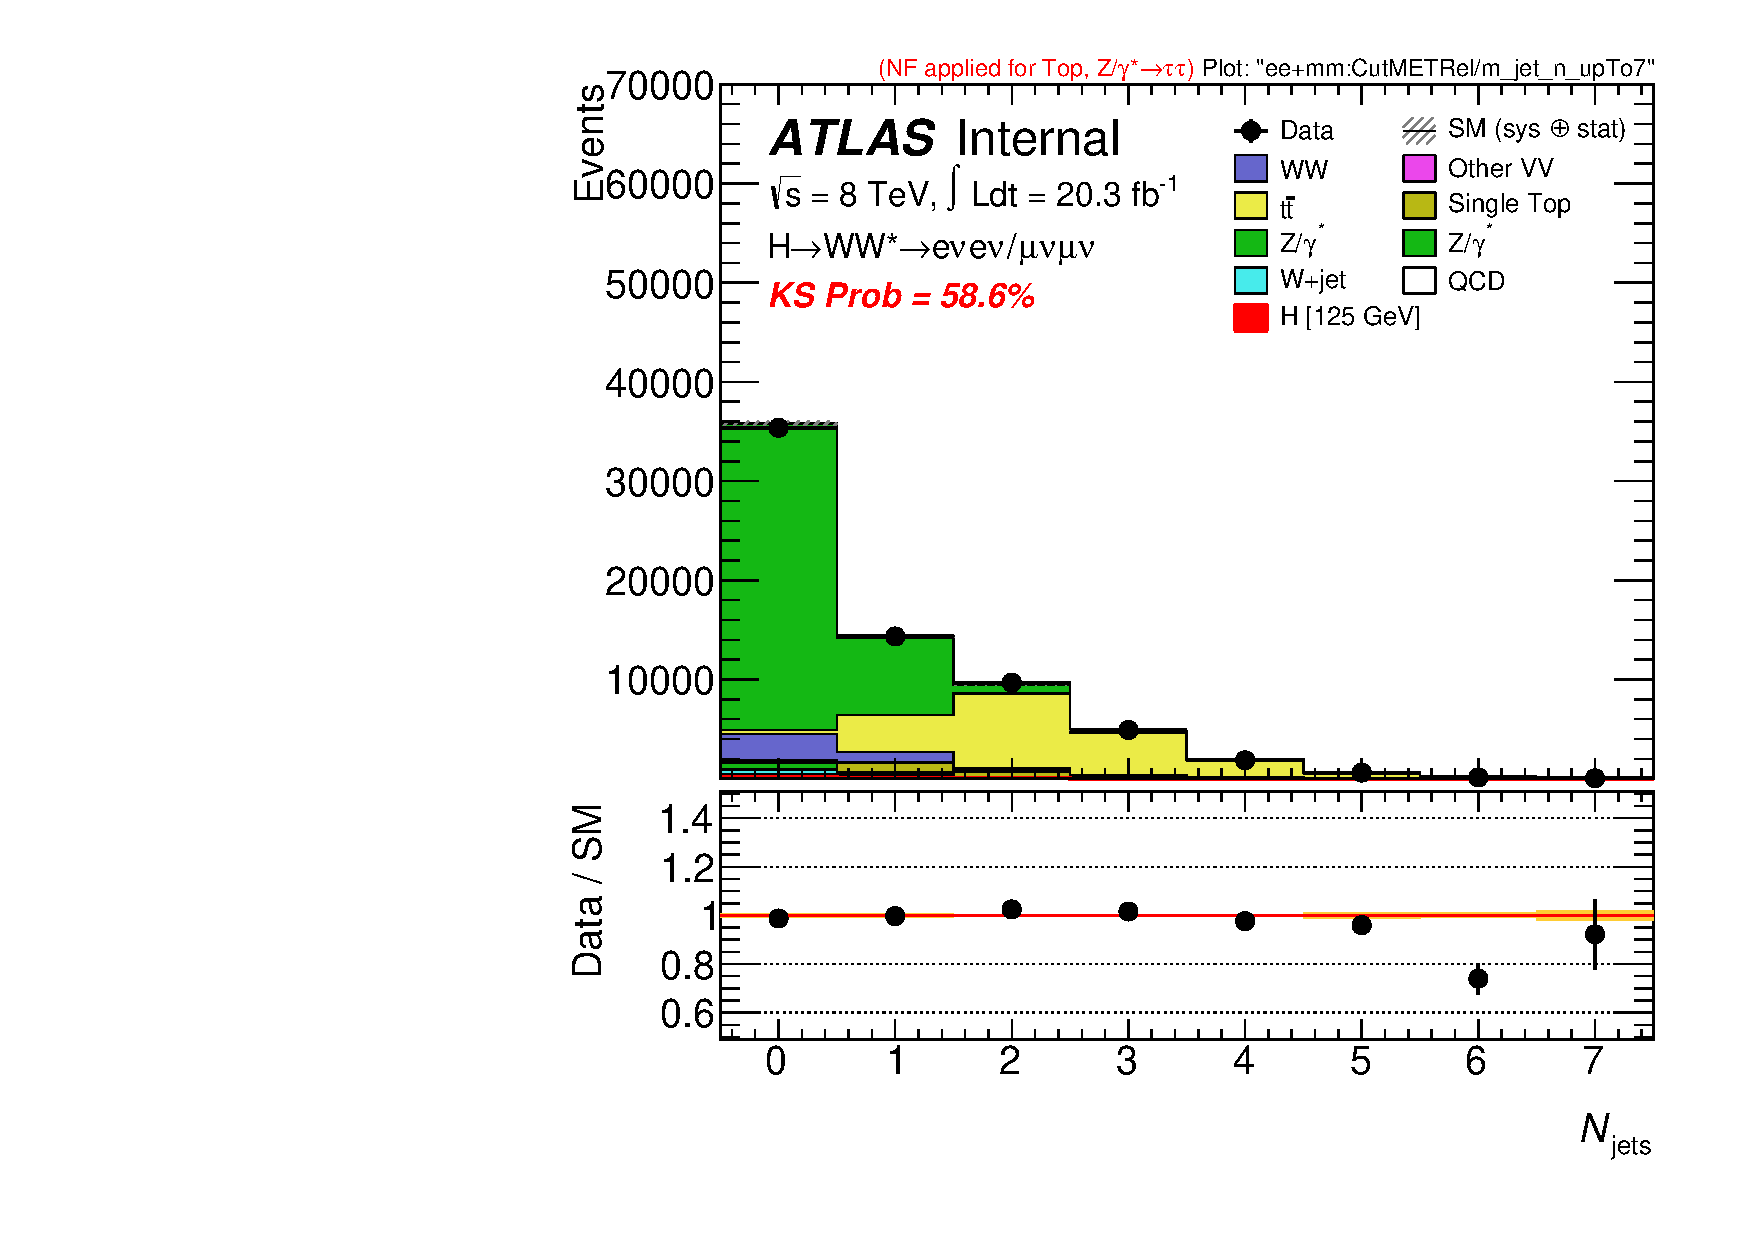
\includegraphics[width=0.495\textwidth]{tex/selection/eemm_CutMETRel_m_jet_n_upTo7_mh125_lin}
	\caption{Jet multiplicity distribution in the \emch/\mech (left) and \eech/\mmch (right) 
	channels. These are made following the pre-selection.}
	\label{fig:sel:njets}
\end{figure}



\subsection{\HWWlvlv decay topology}
\label{sec:selection:higgs_decay}

The discrimination of \HWW signal from irreducible backgrounds that also feature a \WW pair 
is a problem common to all jet bins. Thus, the topology of the \HWWlvlv decay is discussed 
before continuing with the event selection.

Firstly, the spin-0 nature of the Higgs boson and the \VminusA structure of the weak 
interaction (see \Section~\ref{sec:ewsb}) imply that a small opening angle between the 
two leptons is preferred. This follows from spin conservation and the extremely small 
masses of the neutrinos. Consequently, the mass of the dilepton system, \mll, is also 
small. This follows from $m_{\Plepton\Plepton}^2 \simeq m_{\Plepton_1}^2 + 
m_{\Plepton_2}^2 + 2 E_{\Plepton_1} E_{\Plepton_2} \parenths{1 - \cos\vartheta}$, where 
$\vartheta$ is the opening angle. Thus, signal events are selected with the criteria 
$\dphill < 1.8$ and \unit{$\mll < 55$}{\GeV}.

Secondly, the invariant mass of the dilepton + dineutrino system should correspond to 
\mH (modified by a Breit-Wigner distribution). Unfortunately, as discussed above, it is 
only possible to infer the \textit{transverse} component of the dineutrino system 
momentum. We therefore construct a transverse mass variable
\begin{equation}
	\mt = \sqrt{\parenths{\etll + \corrtrackmet}^2 - \mods{\ptllvec + \corrtrackmetvec}^2}
\end{equation}
where $E_{\text{T,\HepProcess{\Plepton\Plepton}}}^2 = 
p_{\text{T,\HepProcess{\Plepton\Plepton}}}^2 + m_{\Plepton\Plepton}^2$ and 
\corrtrackmetvec 
is used as it has the best resolution (see \Section~\ref{sec:objects:met}). At 
hadron-level this is an event-by-event lower bound on \mH, though at detector-level the 
sharp cut-off is smeared by the poor \corrtrackmet resolution. This \mt observable is used in 
the statistical fitting procedure.



\subsection{0-jet selection}
\label{sec:selection:0j}

The 0-jet bin is dominated by \DY and \WW backgrounds. A small number of pathological 
events where \metvec is near \ptllvec are rejected by requiring $\dphillmet > \pi/2$.

Considering the \DYll background, the boson \pt will generally be less than the \pt 
threshold used in jet selection, since no jet has been found. Thus, the \DY background is 
greatly reduced by requiring \unit{$\ptll > 30$}{\GeV} (see 
\Figure~\ref{fig:sel:0j:ptll}). In the \eech/\mmch channels only, the \DYll background is 
also suppressed by an additional cut \unit{$\trackmetrel > 40$}{\GeV} (see 
\Figure~\ref{fig:sel:0j:sf_cuts}).

\begin{figure}[t]
	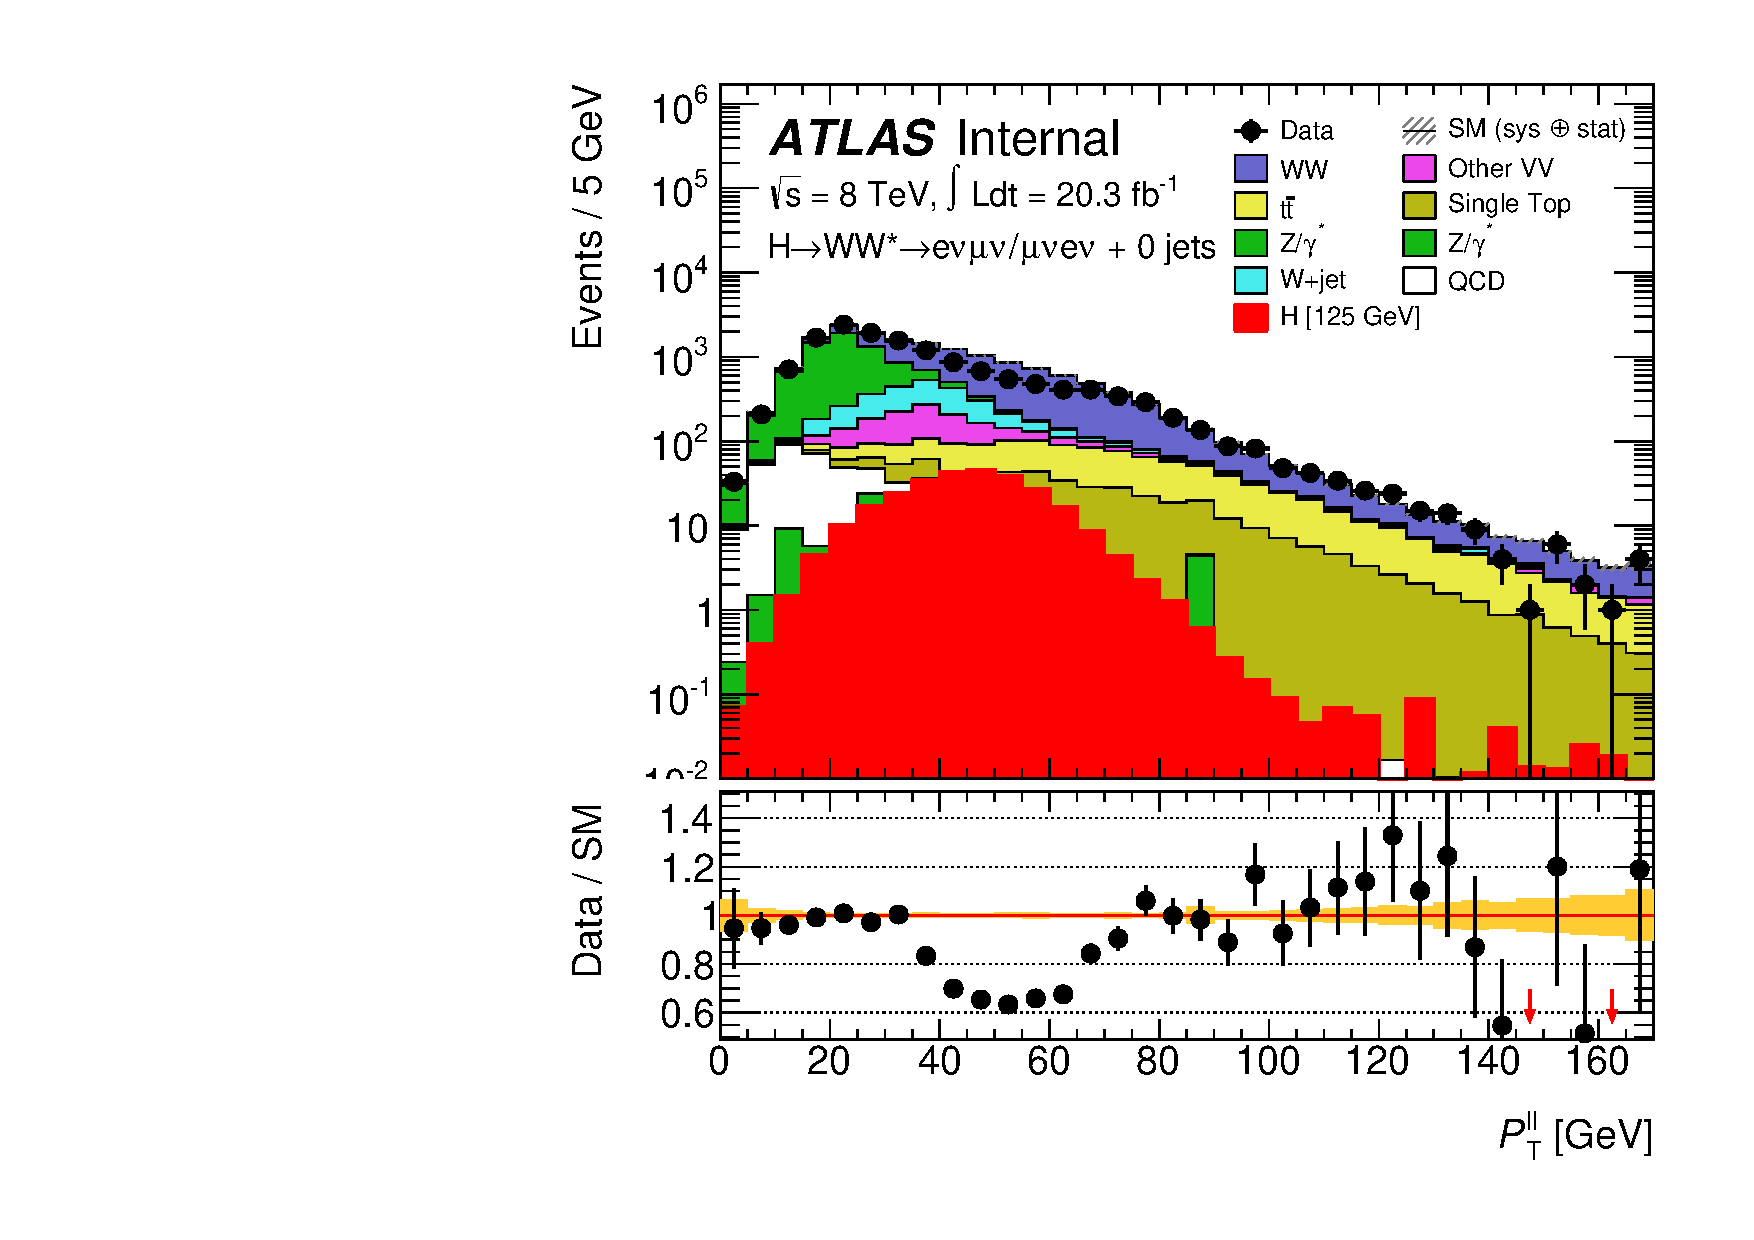
\includegraphics[width=0.495\textwidth]{tex/selection/emme_CutDPhillMET_0jet_Ptll_mh125_log}
	\hfill
	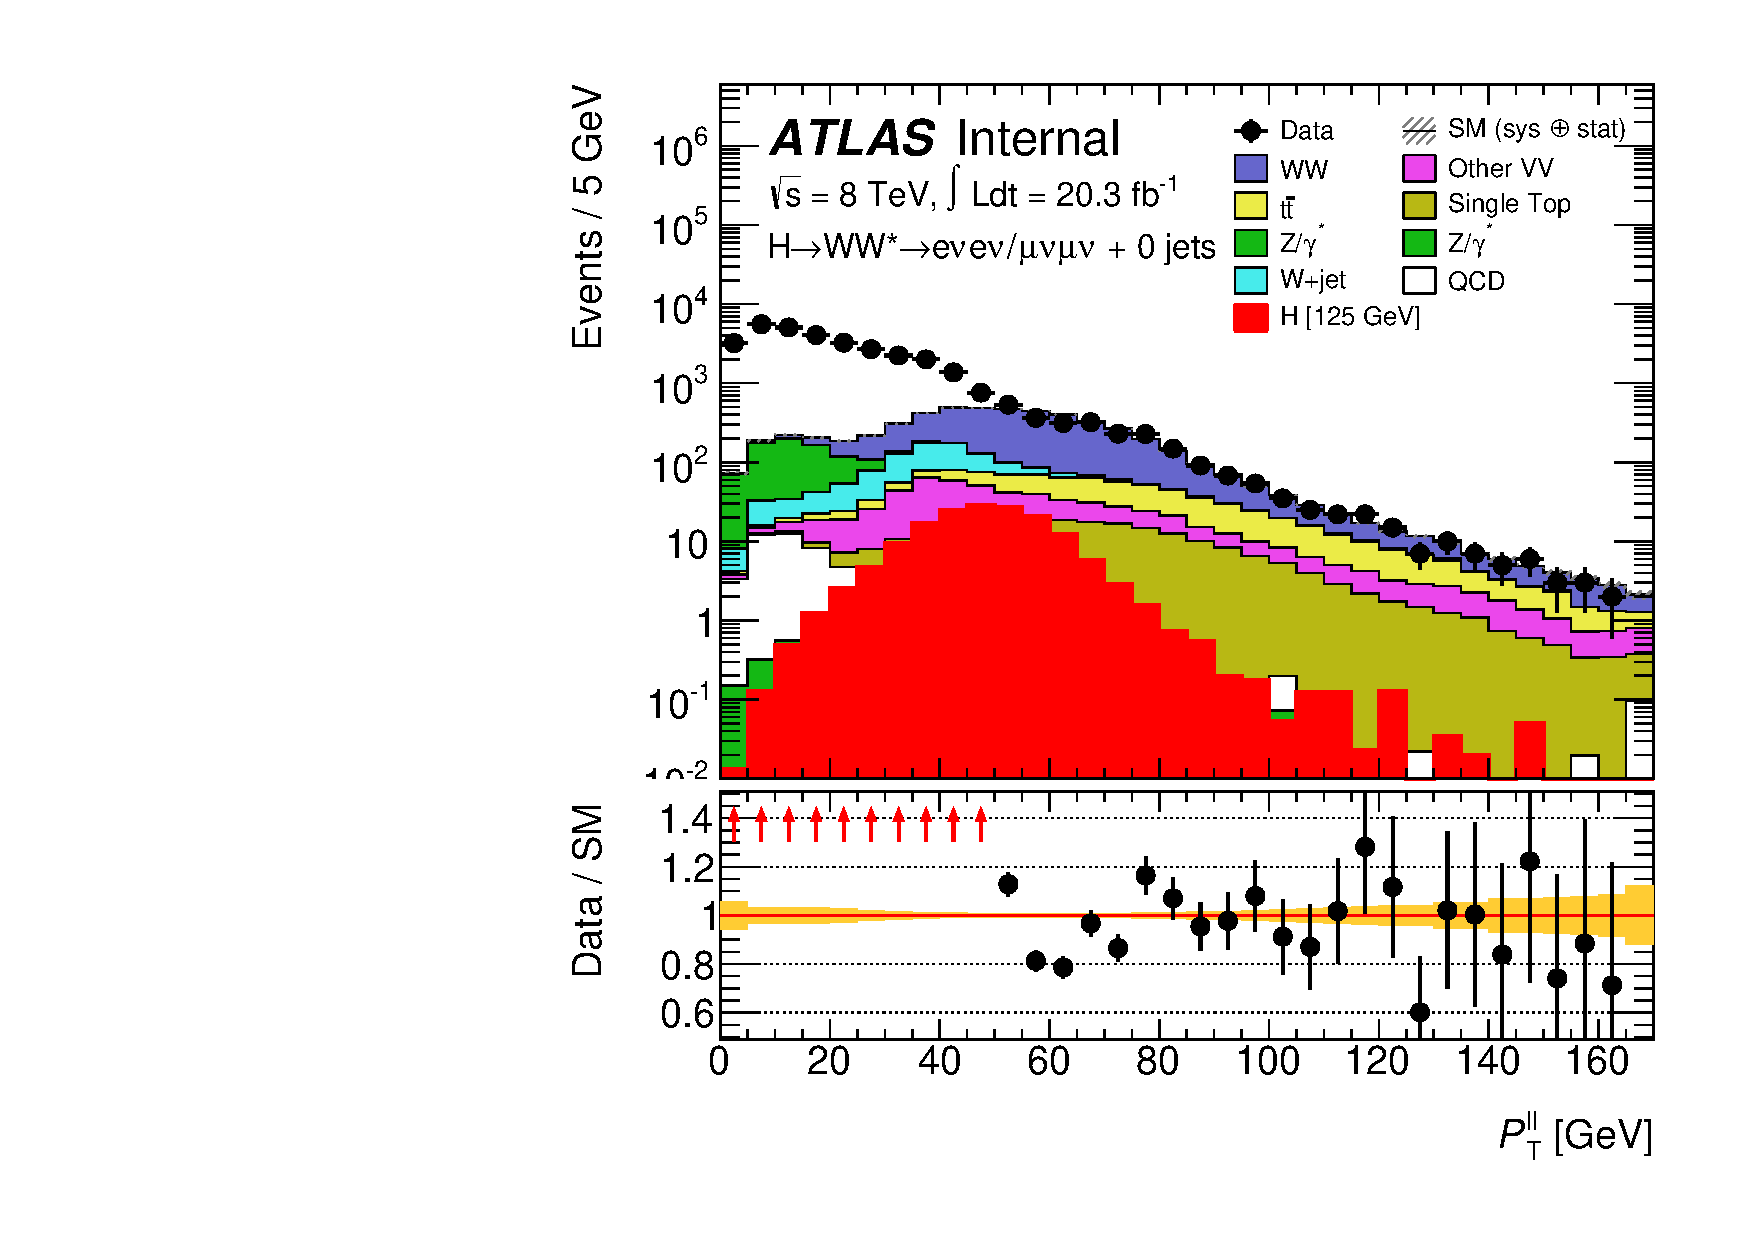
\includegraphics[width=0.495\textwidth]{tex/selection/eemm_CutDPhillMET_0jet_Ptll_mh125_log}
	\caption{The \ptll distribution in the \emch/\mech (left) and \eech/\mmch (right) 
	channels. These are made in the 0-jet bin, after the \dphillmet cut.}
	\label{fig:sel:0j:ptll}
\end{figure}

After the signal topology selection (see \Section~\ref{sec:selection:higgs_decay}), a 
large \DYll background remains in the \eech/\mmch channels, despite the significant \met 
requirements. This can be further suppressed by searching for soft hadronic activity to 
balance the dilepton system. First, jets with \unit{$\pt > 10$}{\GeV} and $\mods{\eta} < 
4.5$ are found (as detailed in \Section~\ref{sec:objects:jets}, minus the JVF cut). 
Then a discriminant is defined
\begin{equation}
	\frecoil = \left. \mods{\sum\limits_{j\text{ in }\wedge} \text{JVF}_{j} \cdot \bvec{p}_{\text{T,}j}} \, \middle/ \ptll \right.
	\label{eq:frecoil}
\end{equation}
where $\wedge$ is the detector quadrant centred on $-\ptllvec$. This is essentially the 
fraction of \ptll that can be balanced by soft hadronic activity in the opposing quadrant,
and so is larger in \DYll than processes with neutrinos. We require $\frecoil < 0.1$ in 
the \eech/\mmch channels (see \Figure~\ref{fig:sel:0j:sf_cuts}). \frecoil is also 
instrumental in estimating the \DYll background, and shall be revisited in 
\Section~\ref{sec:dy}.

\begin{figure}
	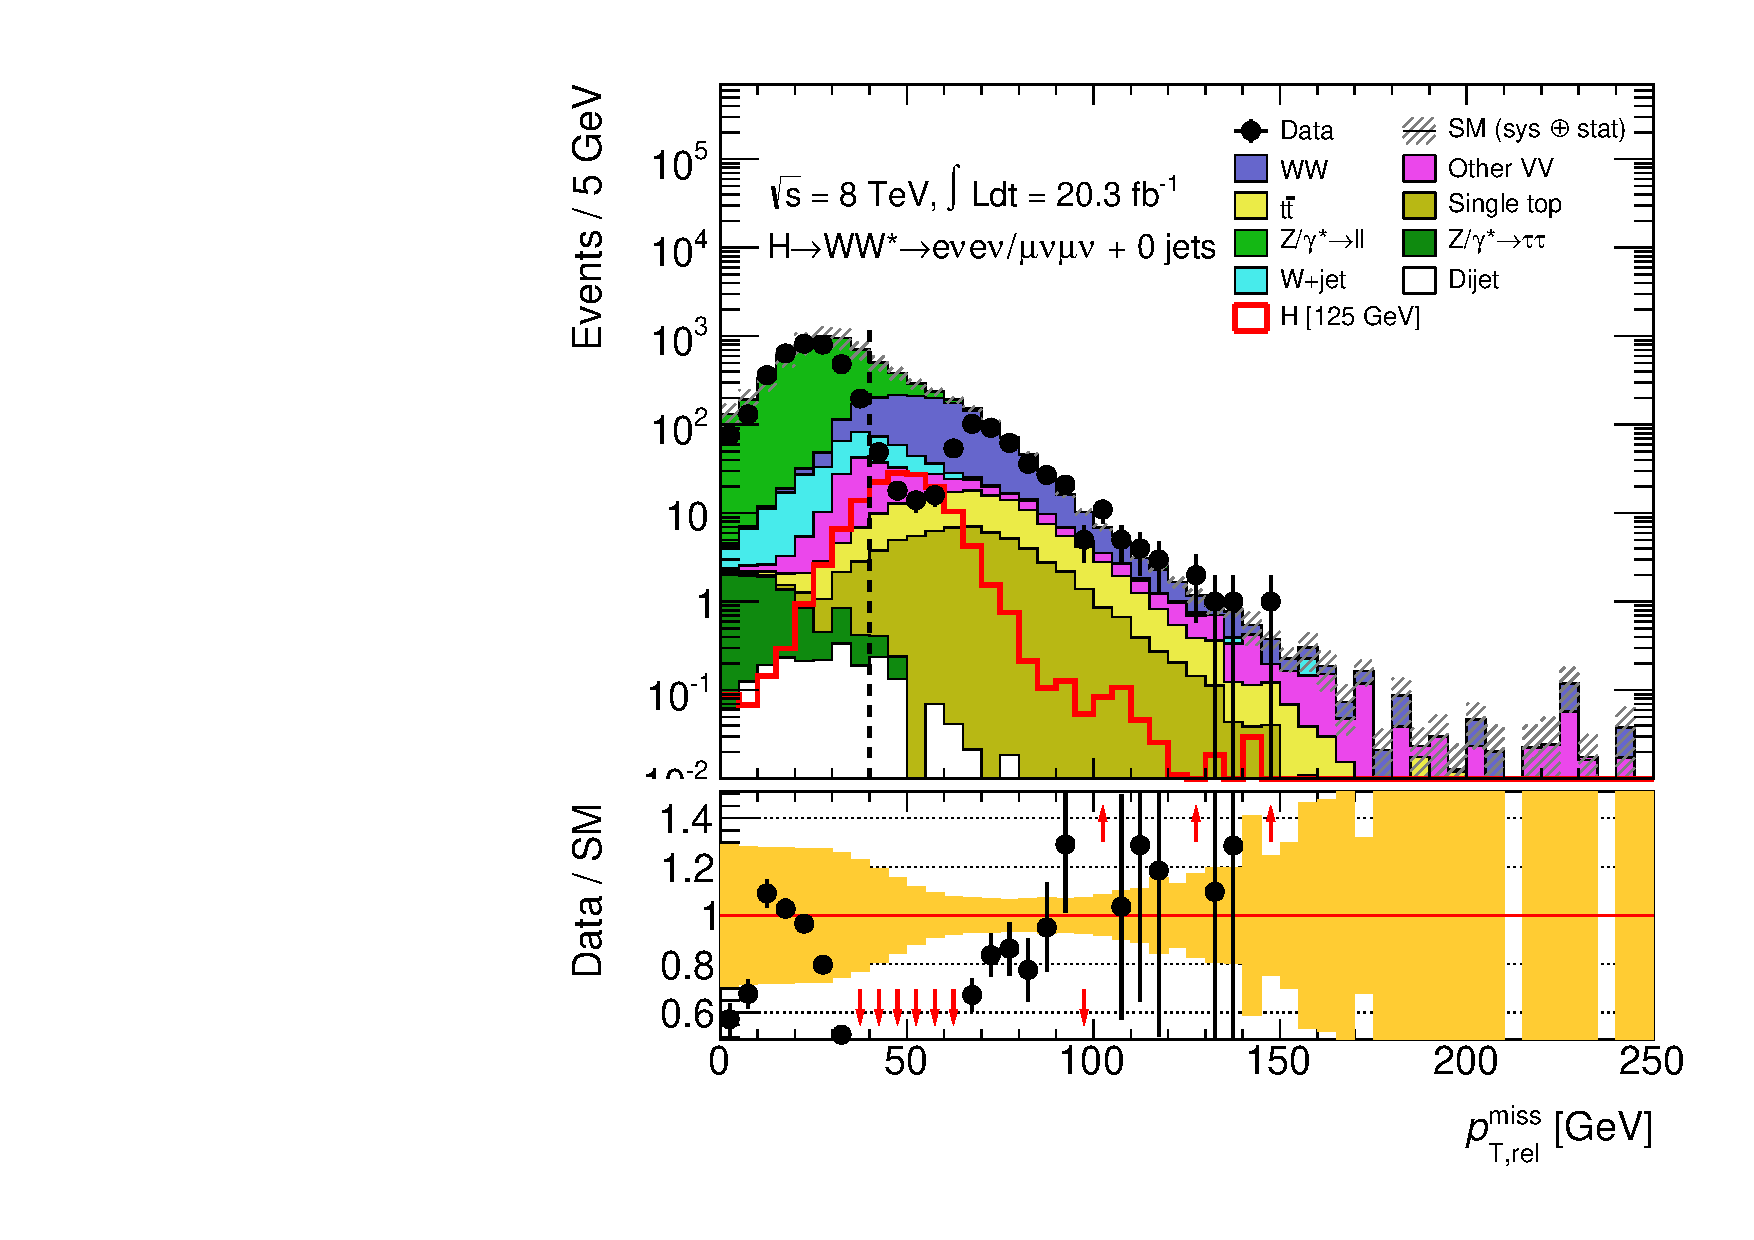
\includegraphics[width=0.495\textwidth]{tex/selection/eemm_CutTopoMll_0jet_METRel_TrackHWW_mh125_log}
	\hfill
	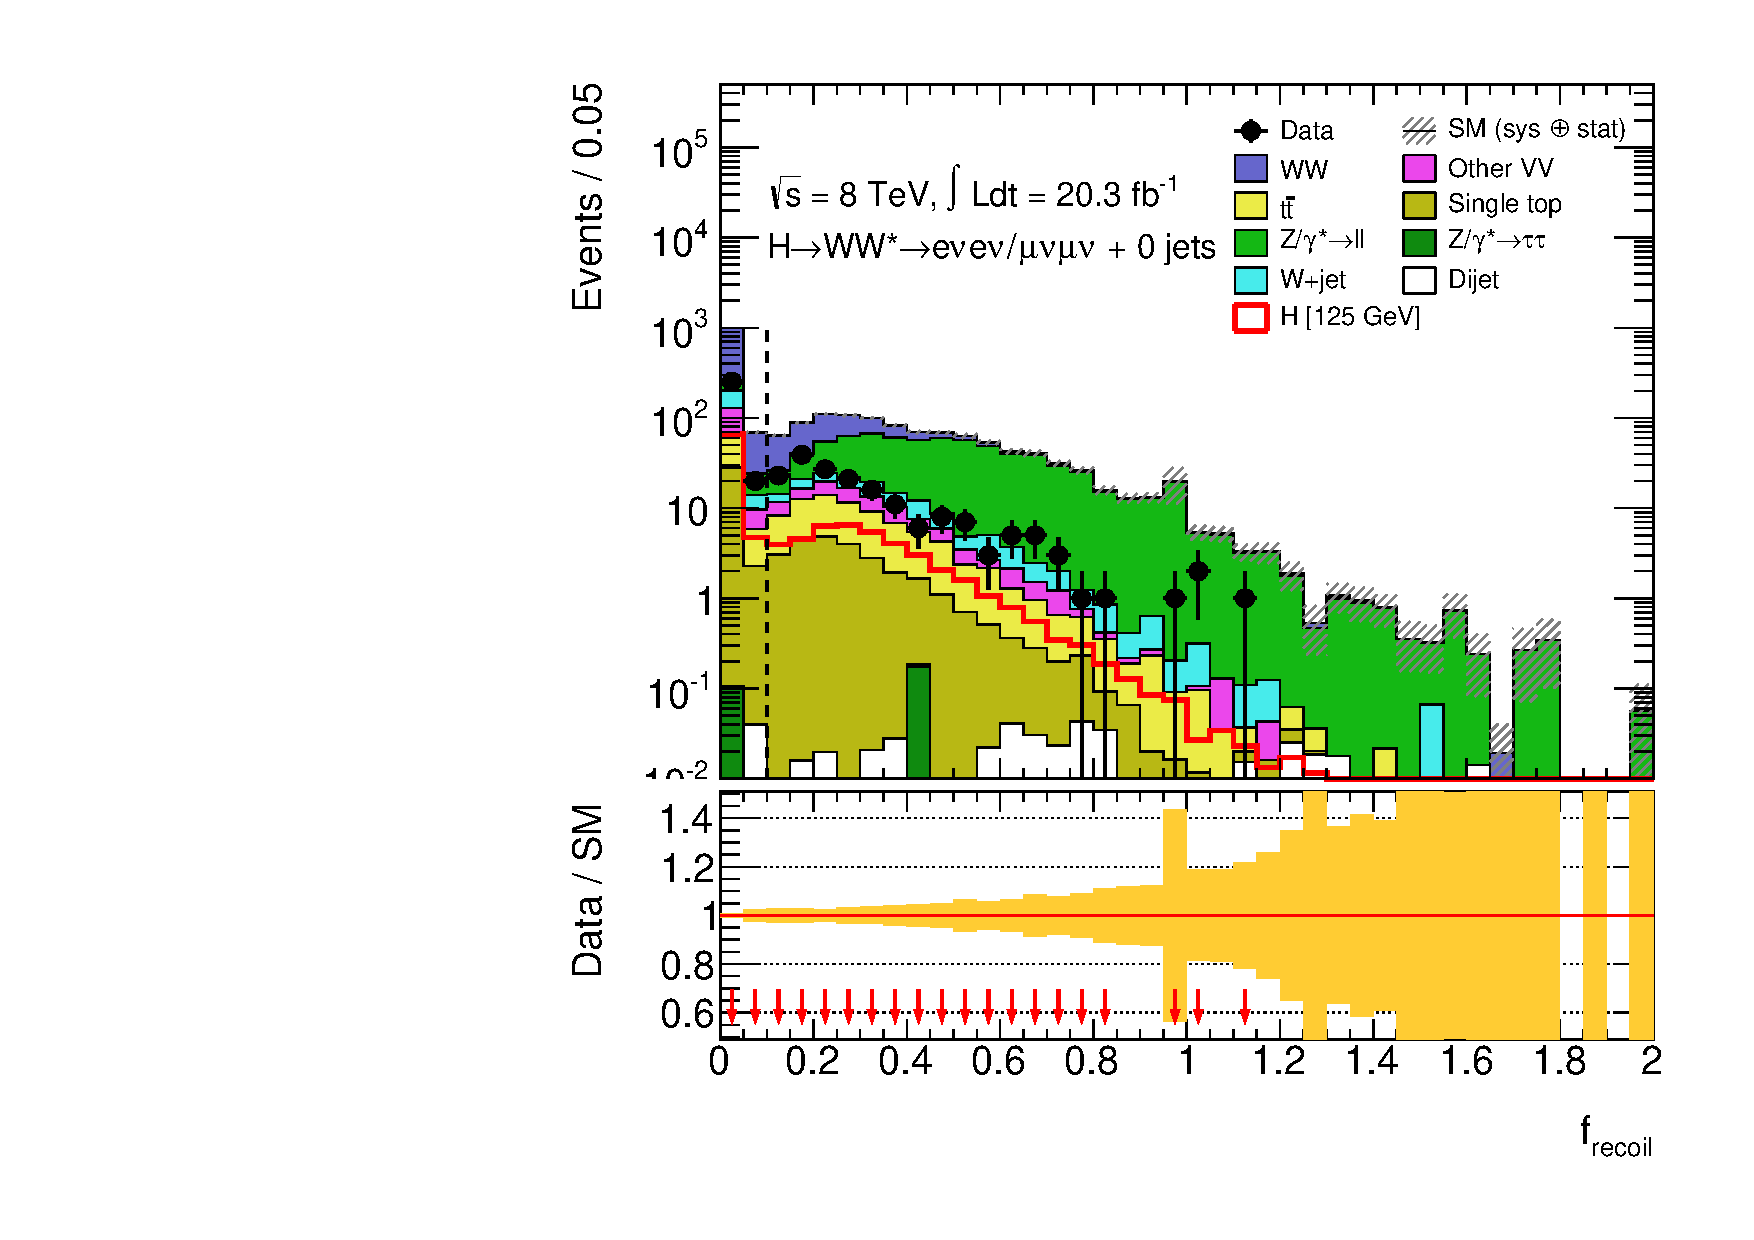
\includegraphics[width=0.495\textwidth]{tex/selection/eemm_CutTopoDPhill_0jet_f_recoil_mh125_log}
	\caption{The \trackmetrel (left) and \frecoil (right) distributions in the \eech/\mmch 
	channels, directly before they are cut upon.}
	\label{fig:sel:0j:sf_cuts}
\end{figure}

The event yields of the 0-jet selection are provided in \Appendix~\ref{app:sr_yields}, 
and the \mt distributions of the selected events are shown in \Figure~\ref{fig:sel:0j:mt}.

\begin{figure}
	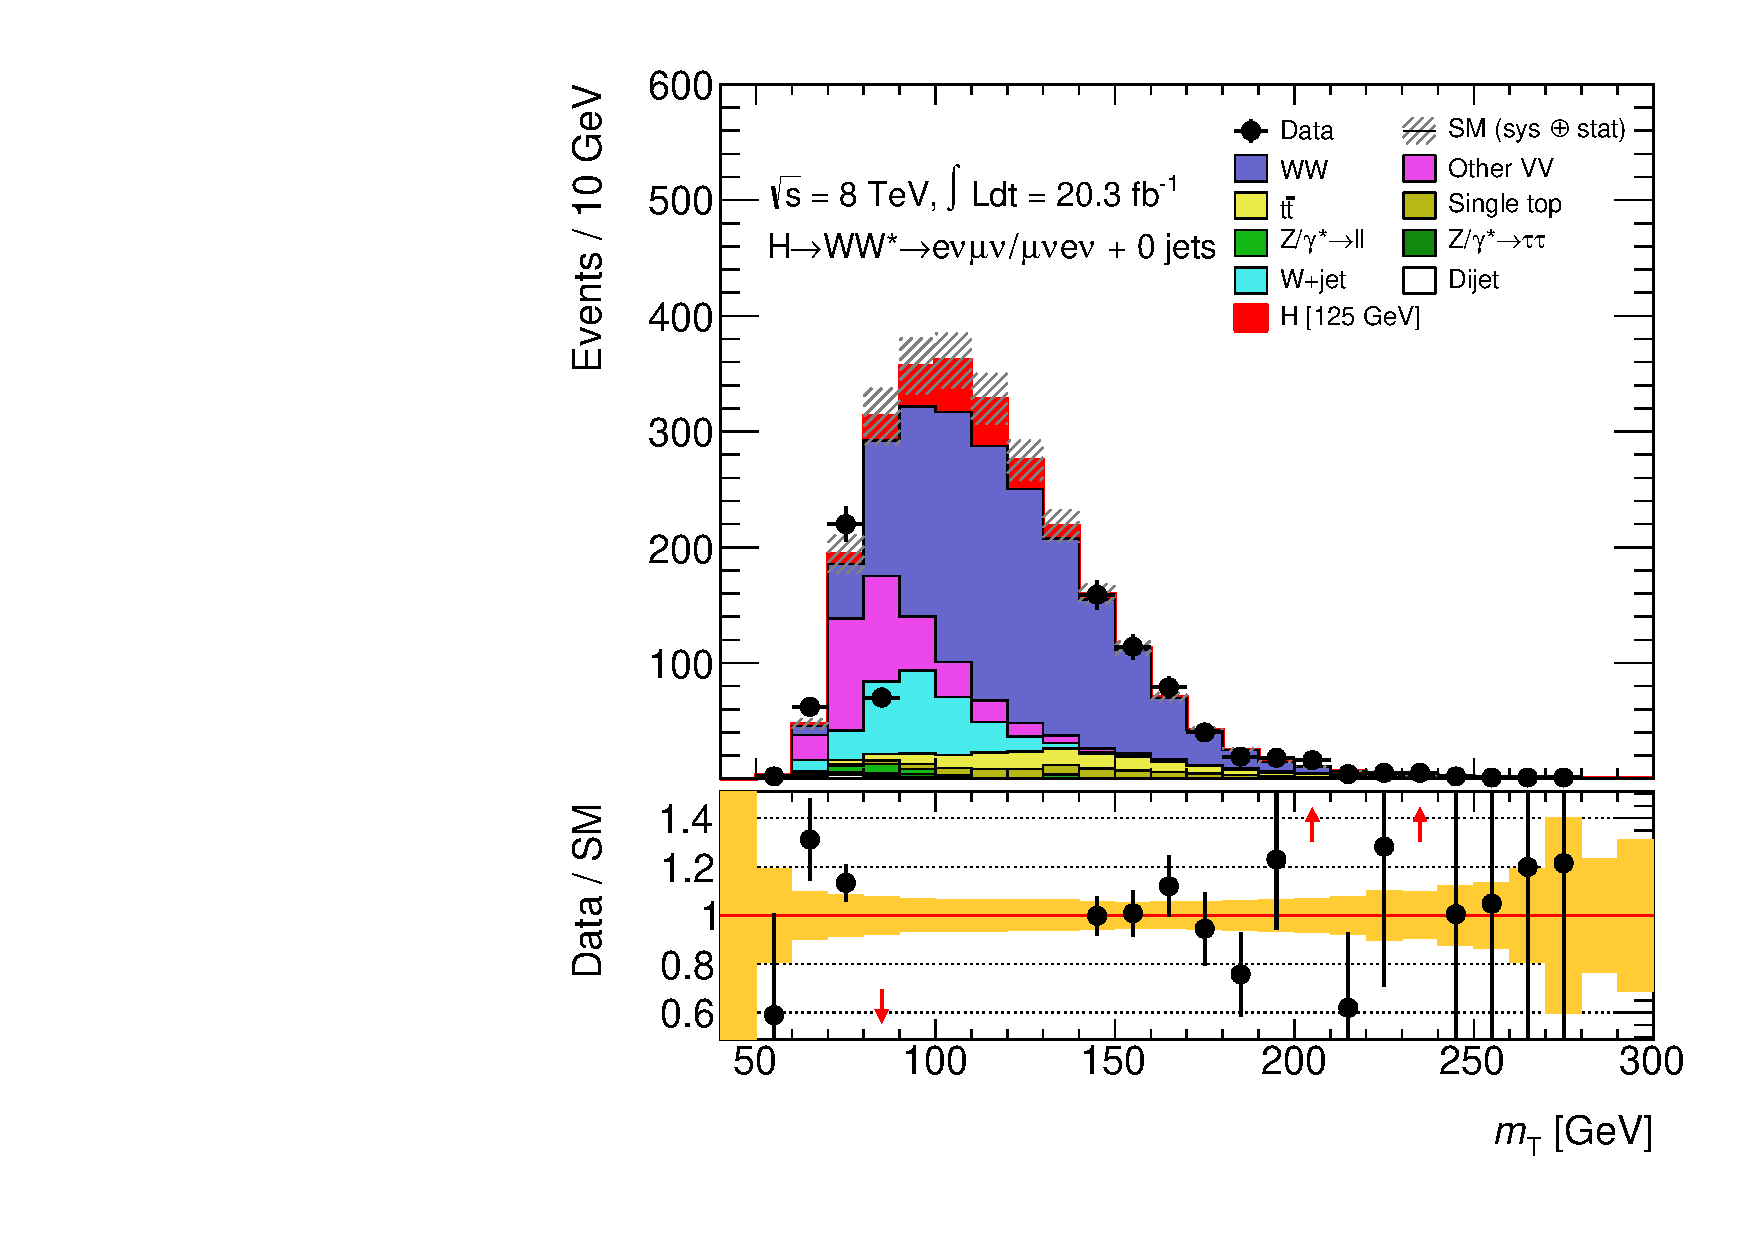
\includegraphics[width=0.495\textwidth]{tex/selection/emme_CutFRecoil_0jet_MT_TrackHWW_Clj_mh125_lin}
	\hfill
	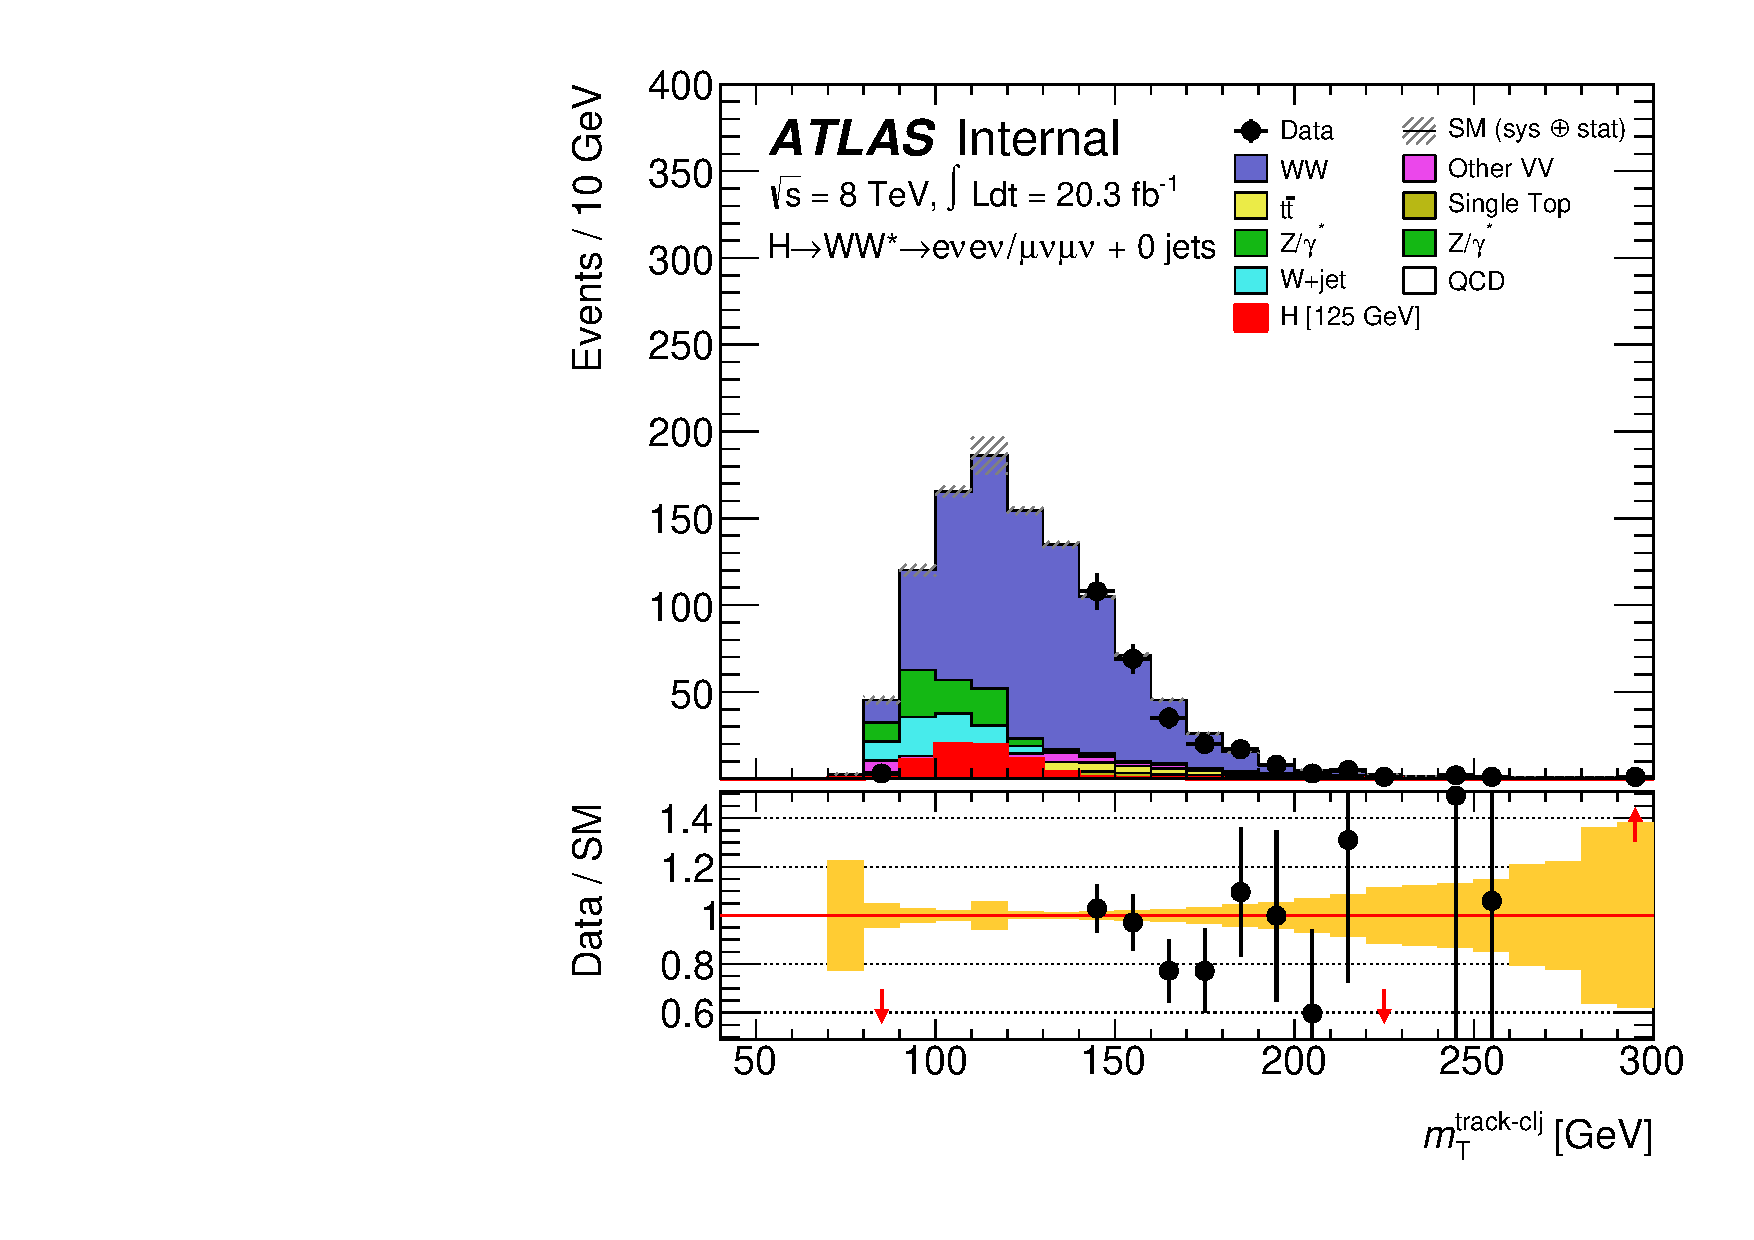
\includegraphics[width=0.495\textwidth]{tex/selection/eemm_CutFRecoil_0jet_MT_TrackHWW_Clj_mh125_lin}
	\caption{The \mt distribution of the selected 0-jet events, in the \emch/\mech (left) and 
	\eech/\mmch (right) channels.}
	\label{fig:sel:0j:mt}
\end{figure}



\subsection{1-jet selection}
\label{sec:selection:1j}

The 1-jet bin is initially dominated by the \DY and top backgrounds (see 
\Figure~\ref{fig:sel:njets}), though the top background is efficiently reduced by vetoing 
events containing a \Pbottom-tagged jet with \unit{$\pt > 20$}{\GeV} (see 
\Section~\ref{sec:objects:bjets}).

In order to reduce the dijet background, which has a large uncertainty, two single-lepton 
transverse mass variables are constructed
\begin{equation}
	m_{\text{T,}\Plepton_i} = \sqrt{2 \, p_{\text{T,}\Plepton_i} \, \corrtrackmet 
	\sqbracs{1 - \cos\Delta\phi\parenths{\Plepton_i, \corrtrackmet}}} \,.
\end{equation}
Their maximum, \maxmtw, tends to peak at lower values for processes with fake \met (see 
\Figure~\ref{fig:sel:1j:df_cuts}). Therefore we require \unit{$\maxmtw > 50$}{\GeV} in the 
\emch/\mech channels. In the \eech/\mmch channels, the tighter \met cuts reject the dijet 
background.

\begin{figure}[t]
	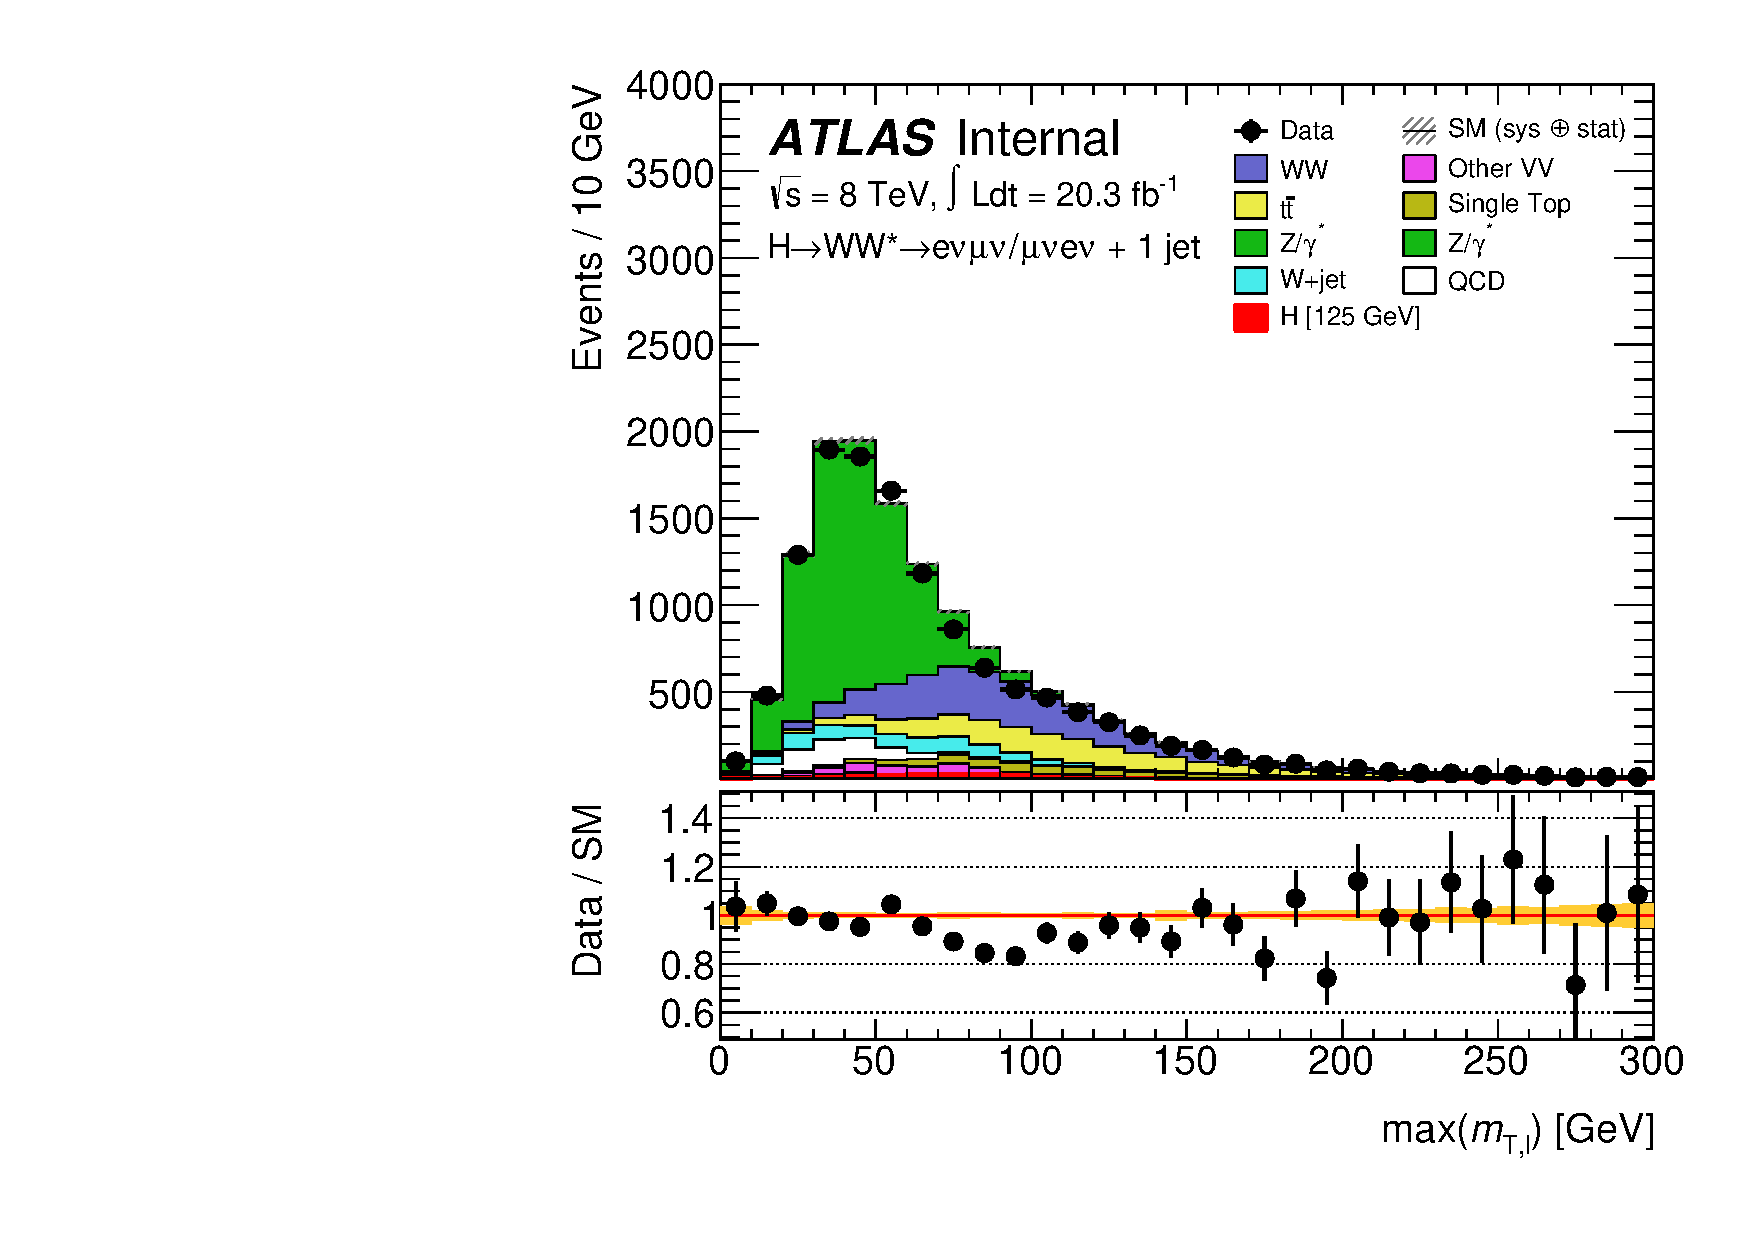
\includegraphics[width=0.495\textwidth]{tex/selection/emme_CutbVeto_1jet_MaxMTW_TrackHWW_Clj_mh125_lin}
	\hfill
	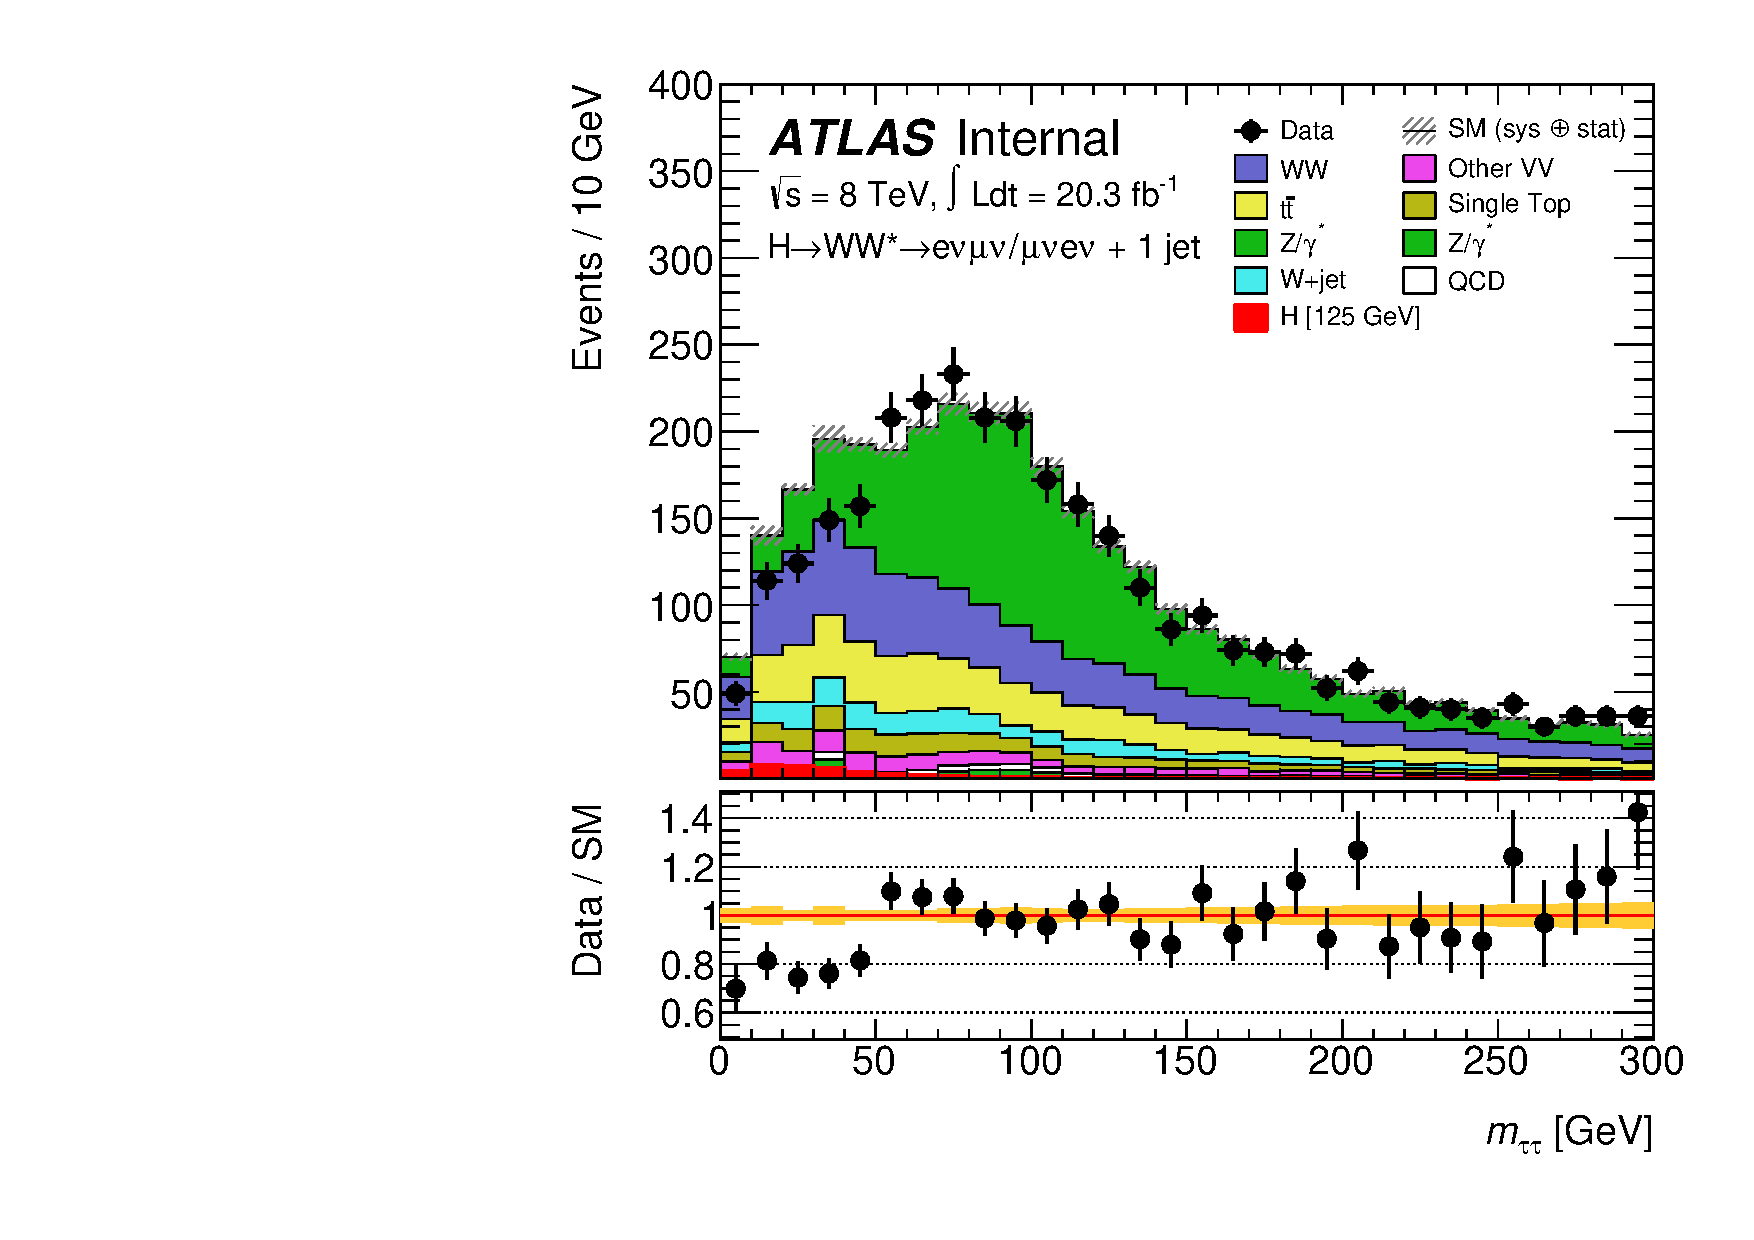
\includegraphics[width=0.495\textwidth]{tex/selection/emme_CutMaxMTlep_1jet_Mtt_TrackHWW_Clj_mh125_lin}
	\caption{The \maxmtw (left) and \mtautau (right) distributions in the \emch/\mech 
	channels, directly before they are cut upon.}
	\label{fig:sel:1j:df_cuts}
\end{figure}

At this stage, the \DYtt background dominates the \emch/\mech channels. To aid 
discrimination, a ditau mass is constructed
\begin{equation}
	\mtautau = 
		\begin{cases}
			\mll \,/ \sqrt{x_1 x_2} &\text{if}~x_1, x_2 > 0 \\
			0 &\text{otherwise}
		\end{cases}
\end{equation}
where $x_i$ is the \pt fraction of the $i$th \Ptau imparted to the $i$th lepton. As $x_i$ 
cannot be directly measured using individual neutrino momenta, \corrtrackmet is split by 
assuming the \Ptau decays collinearly, \ie 
$\Delta\phi\parenths{\Plepton,\HepProcess{\Pnut\Pnulepton}} = 0$. 
This approximation is reasonable since each \Ptau has large \pt. We require 
\unit{$\mtautau < \mZ - 25$}{\GeV} (see \Figure~\ref{fig:sel:1j:df_cuts}). In rare cases 
where the ditau system is poorly reconstructed (\ie $x_i < 0$), the event is accepted.

\begin{figure}[b]
	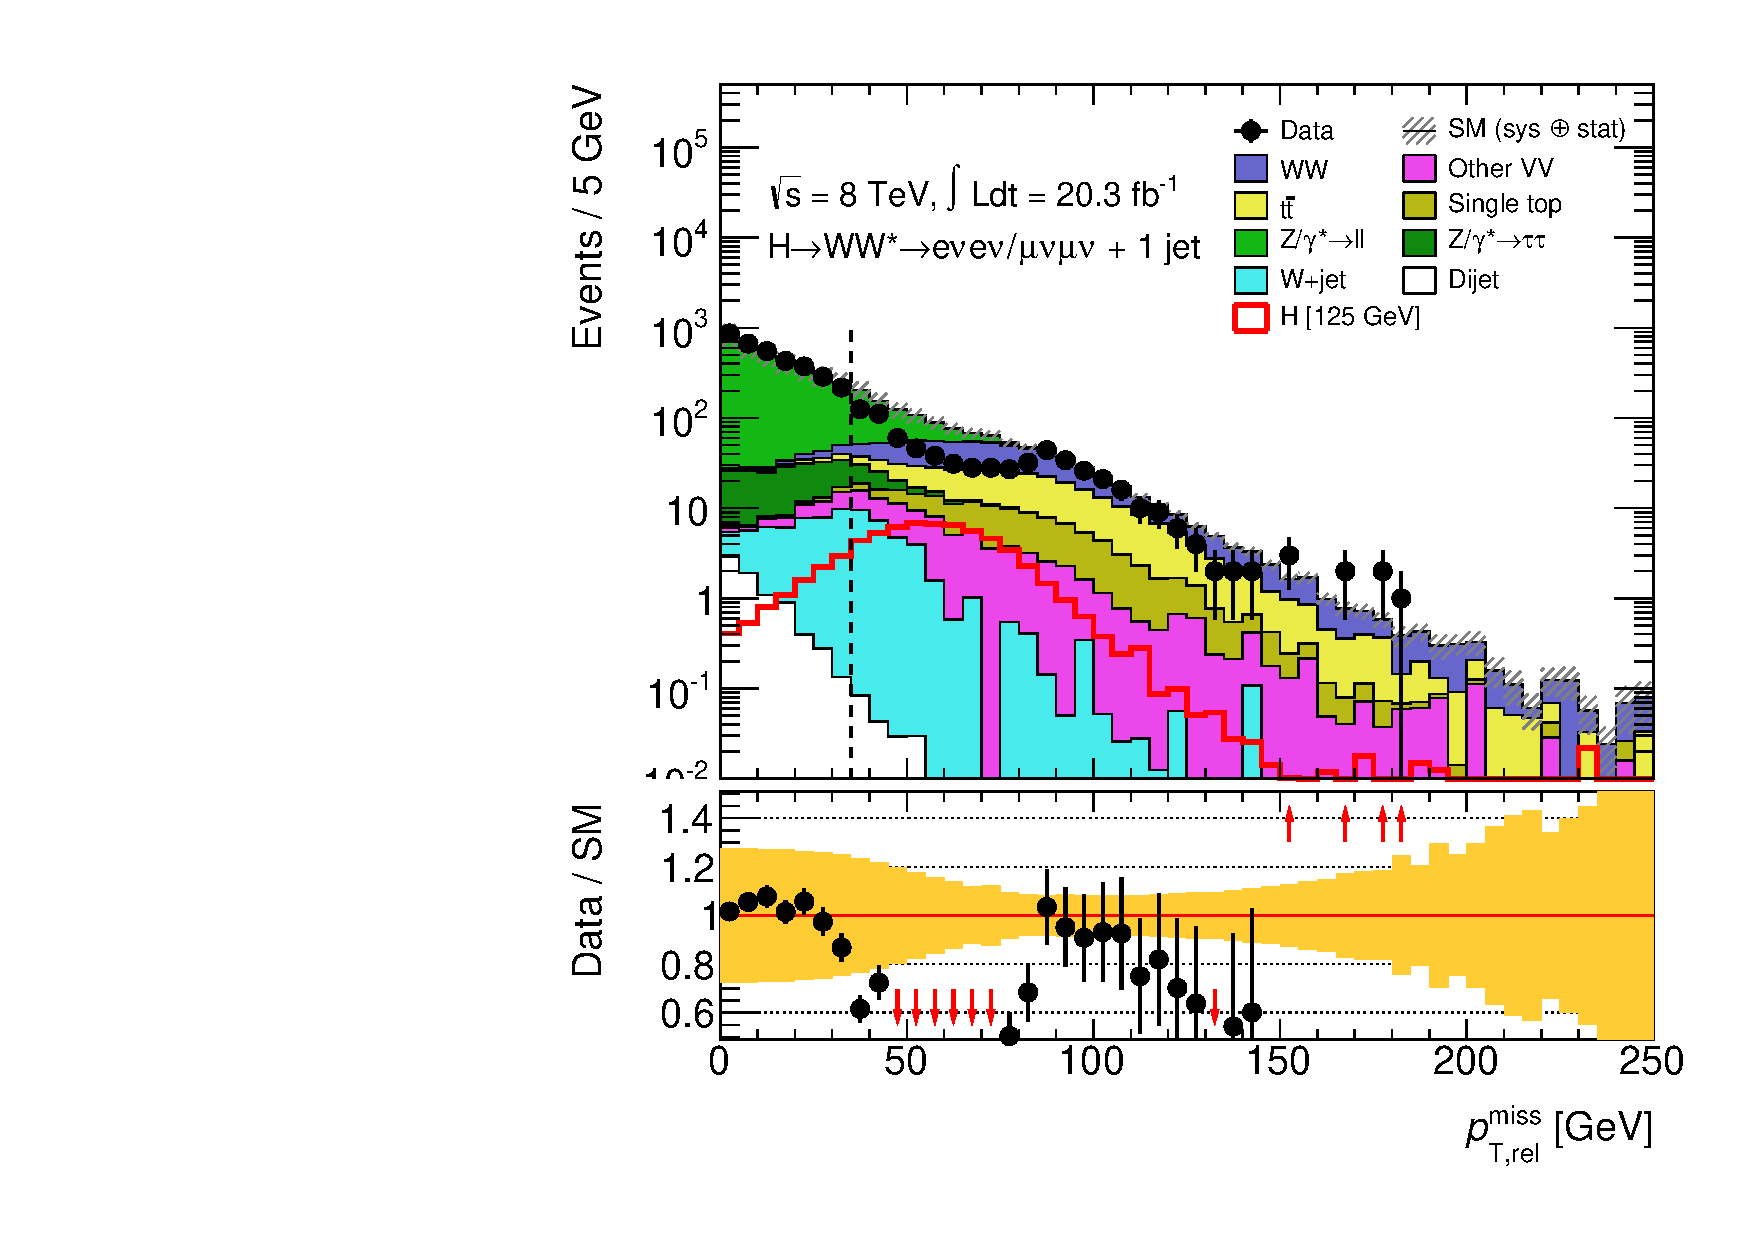
\includegraphics[width=0.495\textwidth]{tex/selection/eemm_CutTopoMll_1jet_METRel_TrackHWW_mh125_log}
	\hfill
	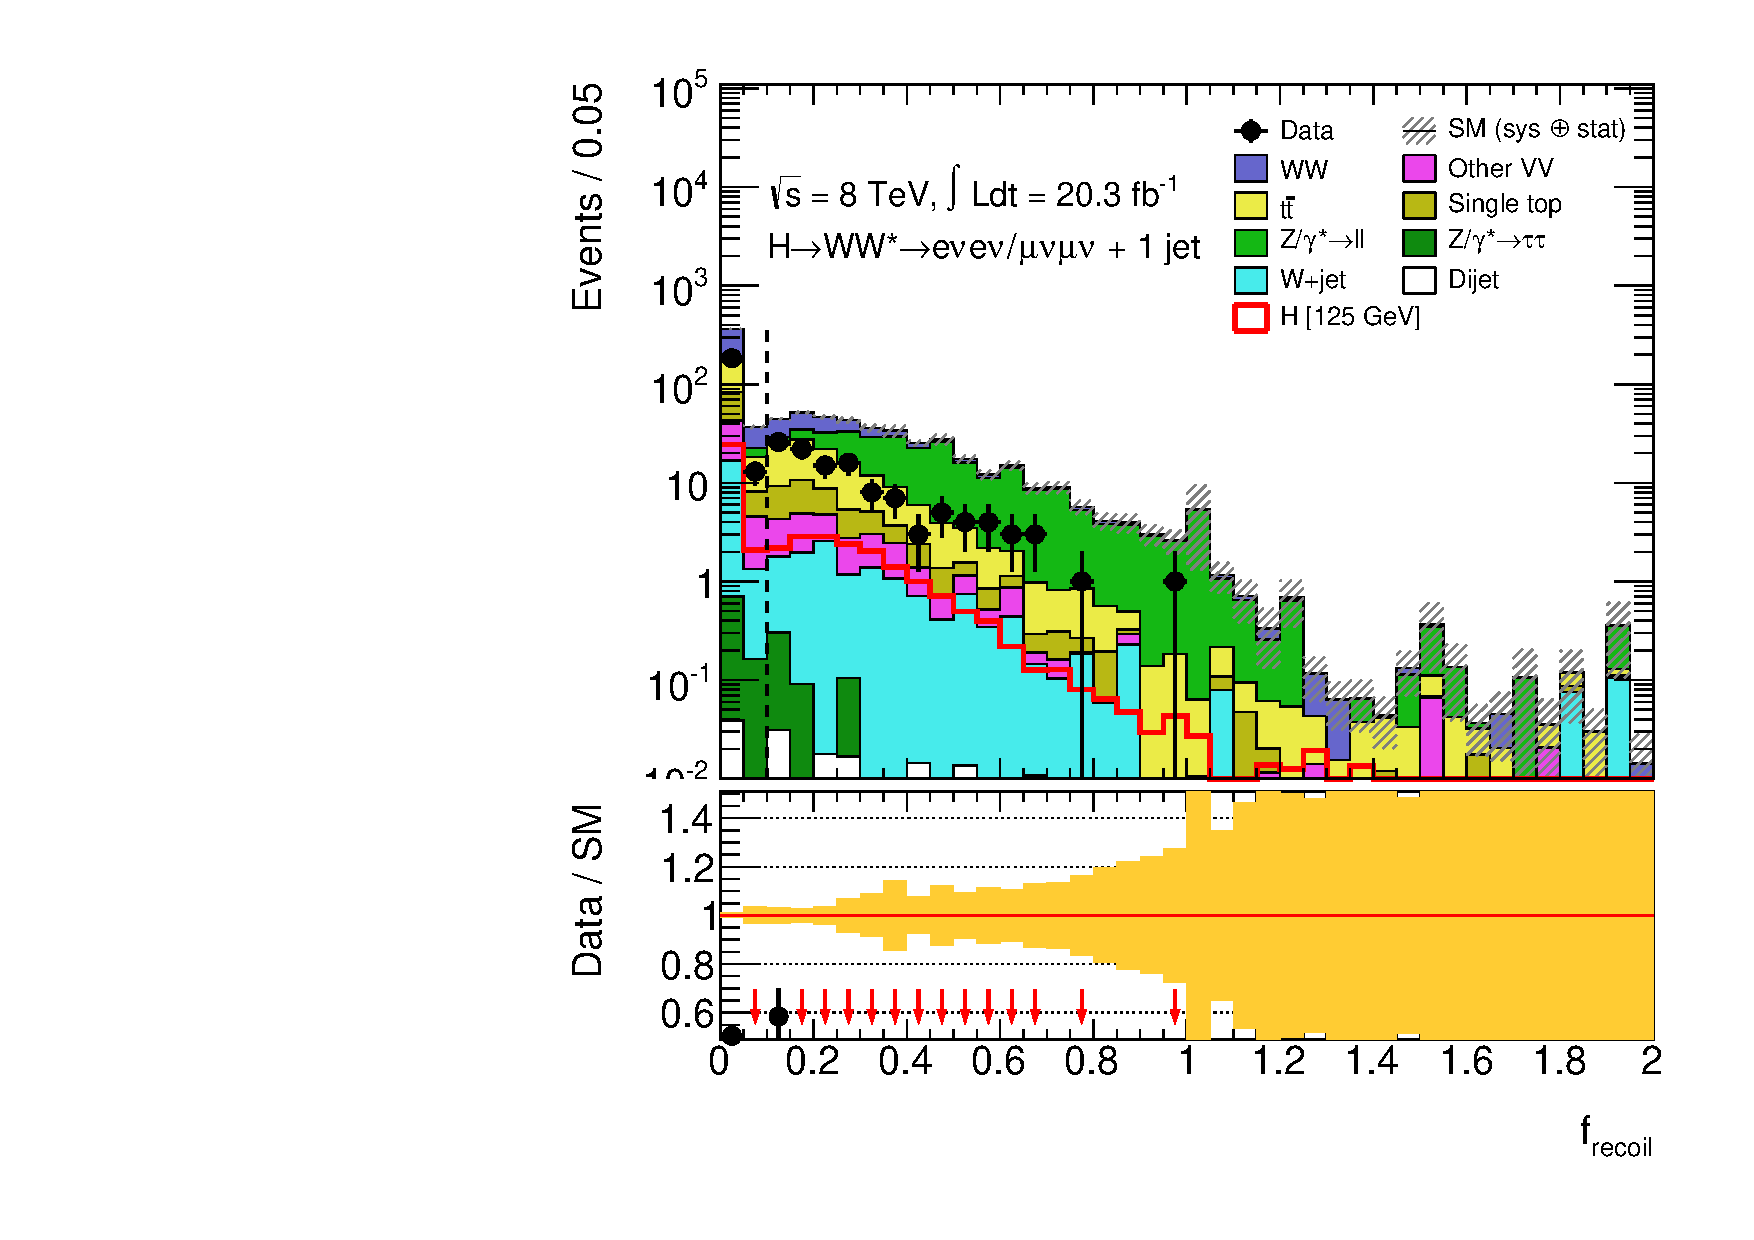
\includegraphics[width=0.495\textwidth]{tex/selection/eemm_CutTopoDPhill_1jet_f_recoil_ext_mh125_log}
	\caption{The \trackmetrel (left) and \frecoil (right) distributions directly 
	before they are cut upon in the \eech/\mmch channels.}
	\label{fig:sel:1j:sf_cuts}
\end{figure}

After the signal topology selection, the \DYll background is suppressed in the 
\eech/\mmch channels by requiring \unit{$\trackmetrel > 35$}{\GeV} and $\frecoil < 0.1$ 
(see \Figure~\ref{fig:sel:1j:sf_cuts}). In the 1-jet bin, the \frecoil definition is 
altered with respect to (\ref{eq:frecoil}): the quadrant $\wedge$ is centred upon 
$-\ptlljvec$ and the denominator becomes \ptllj. This is because a hard jet has been 
found, and so it is the dilepton + jet system that must be balanced by the soft recoil.

The event yields of the 1-jet selection are provided in \Appendix~\ref{app:sr_yields}, 
and the \mt distributions of the selected events are shown in \Figure~\ref{fig:sel:1j:mt}.

\begin{figure}[t]
	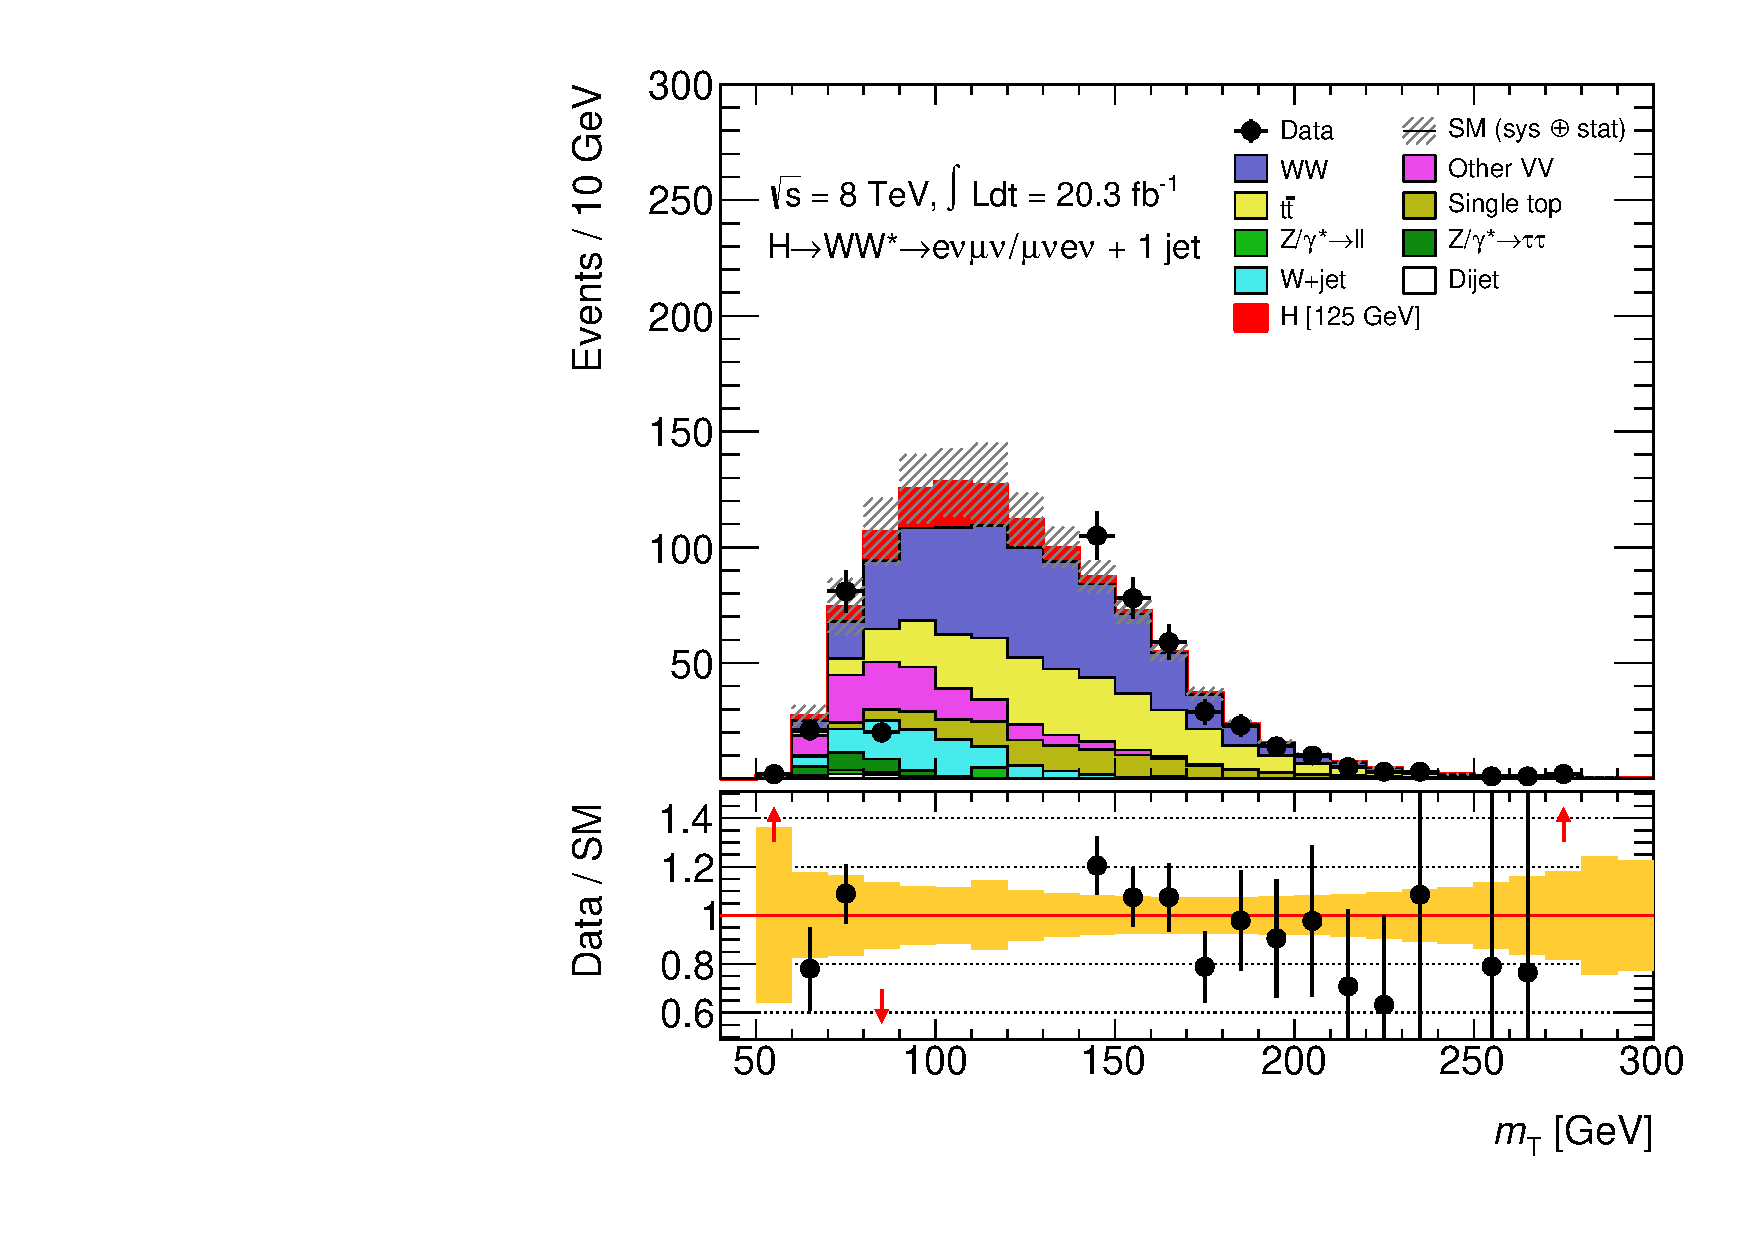
\includegraphics[width=0.495\textwidth]{tex/selection/emme_CutFRecoil_1jet_MT_TrackHWW_Clj_mh125_lin}
	\hfill
	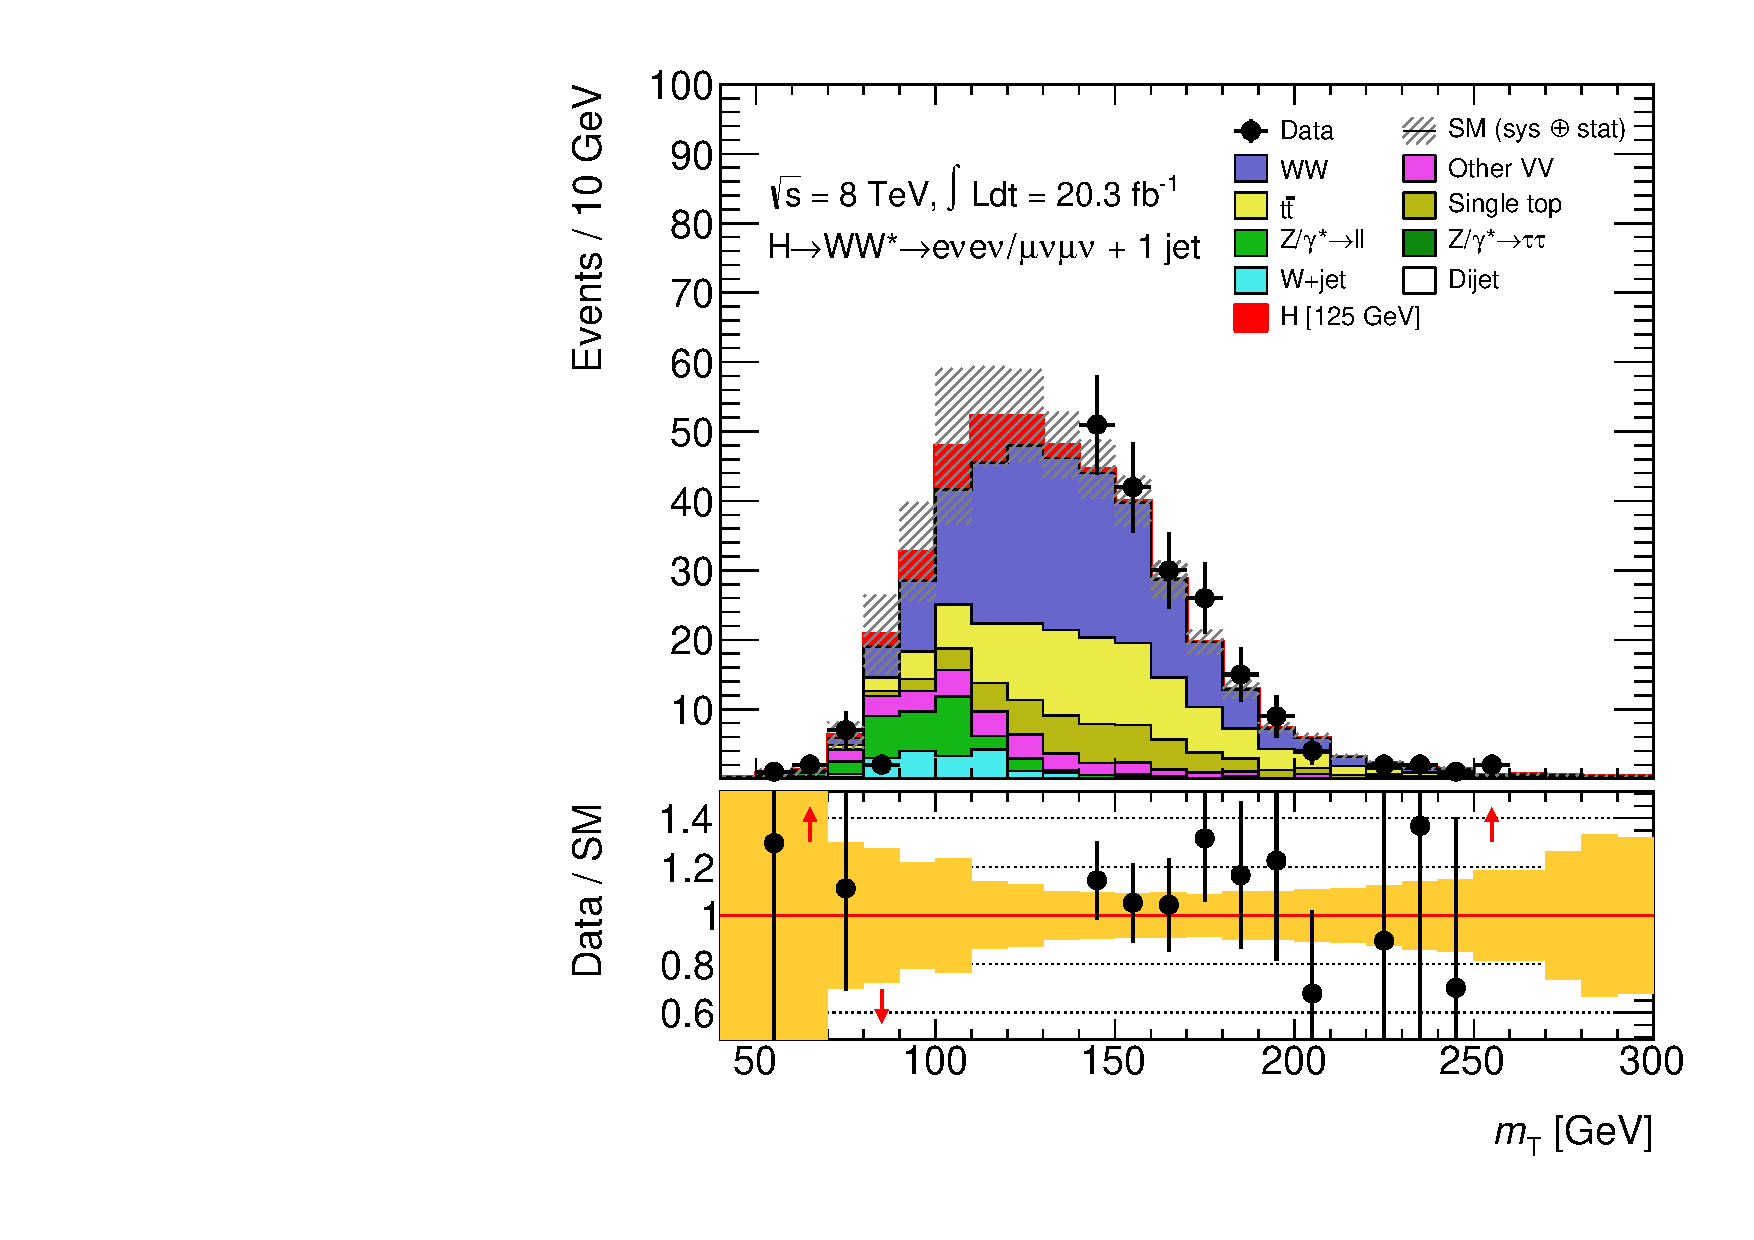
\includegraphics[width=0.495\textwidth]{tex/selection/eemm_CutFRecoil_1jet_MT_TrackHWW_Clj_mh125_lin}
	\caption{The \mt distribution of the selected 1-jet events, in the \emch/\mech (left) and 
	\eech/\mmch (right) channels.}
	\label{fig:sel:1j:mt}
\end{figure}



\subsection{\twojet selection}
\label{sec:selection:2j}

Only the \emch/\mech channels are used in the \twojet bin, which is dominated by top 
background (see \Figure~\ref{fig:sel:njets}). In the following, observable definitions using 
only two jets refer to the two hardest jets. As in the 1-jet bin, the top background is 
greatly suppressed by vetoing events featuring a \Pbottom-tagged jet with 
\unit{$\pt > 20$}{\GeV} (see \Figure~\ref{fig:sel:2j:df_cuts}). Also, the \DYtt background is 
again suppressed by the requirement \unit{$\mtautau < \mZ - 25$}{\GeV} (see 
\Figure~\ref{fig:sel:2j:df_cuts}).

\begin{figure}[t]
	\includegraphics[width=0.495\textwidth]{tex/selection/emme_CutFailVBF_2jetincl_nJets_Pt20_MV1_85_mh125_lin}
	\hfill
	\includegraphics[width=0.495\textwidth]{tex/selection/emme_CutFailVBFbVeto_2jetincl_Mtt_TrackHWW_Clj_mh125_lin}
	\caption{The \nbjets (left) and \mtautau (right) distributions directly 
	before they are cut upon in the \emch/\mech channels.}
	\label{fig:sel:2j:df_cuts}
\end{figure}

At this point, it is necessary to contextualise the analysis. Although this thesis 
describes the search for the ggF production mode, searches for the other production modes 
(see \Section~\ref{sec:properties}) are also performed by the ATLAS collaboration. To 
simplify the statistical combination of these searches, it is helpful to avoid overlap 
between their signal regions. This is particularly important for the \twojet bin.

The VBF production mode features two outgoing quarks at LO (see \Figure~\ref{fig:feyn:VBF}). 
Therefore the \twojet bin is the starting point for the VBF selection. However, the 
absence of colour exchange between the quarks leads to dramatically different event 
topologies compared to ggF events in the \twojet bin; VBF events feature two high-\pt 
jets, separated by a large rapidity gap devoid of hadronic activity. Thus, events 
containing a softer jet with \unit{$\pt > 20$}{\GeV} within this rapidity gap are removed 
from the VBF selection. This is the \textit{central jet veto} (CJV). The VBF selection 
also requires that the leptons lie within this rapidity gap, since the Higgs boson is 
generally produced centrally. This is the \textit{outside lepton veto} (OLV). Finally, a 
boosted decision tree (BDT) \cite{TMVA} is trained to discriminate VBF events based upon 
eight input variables:

\begin{listliketab}
	\begin{tabular}{Ll@{\hskip 0.3in}llll}
		\textbullet & VBF topology:    & \mjj, &\dyjj, &$\eta_{\Plepton}$ centrality, &$\sum_{\Plepton, j} m_{\Plepton j}$ \\
		\textbullet & \HWW decay:      & \mll, &\dphill, &\mt \\
		\textbullet & top suppression: & \pttot \\
	\end{tabular}
\end{listliketab}

\noindent
$\eta_{\Plepton}$ centrality characterises how close the leptons are to the jets. 
$\sum_{\Plepton, j} m_{\Plepton j}$ sums the masses of the four lepton + jet systems 
possible with the two hardest jets, which is higher in VBF events due to the large 
separations involved. \pttot is the sum of \corrtrackmetvec and the \ptvec of each lepton 
and jet, capturing the soft hadronic recoil, which is larger in top background events. 
The BDT scores events between 100\% signal-like ($+1$) and 100\% background-like ($-1$), 
where ggF is considered a background. Events with a score greater than $-0.48$ are selected 
for the VBF analysis.

Another search considers the \WH and \ZH production modes (collectively known as \VH), 
where the vector boson decays hadronically (see \Figure~\ref{fig:feyn:VH}). Again, the 
\twojet bin is the starting point for this selection. As with VBF, the jet kinematics can 
be used to distinguish this from ggF. First, a small rapidity gap is required, $\dyjj < 1.2$. 
Second, the dijet system must have a mass corresponding to a \PW or \PZ boson, 
\unit{$\mods{\mjj - 85} < 15$}{\GeV}.

To maintain orthogonality with the VBF and \VH analyses, the ggF analysis requires that 
events in the \twojet bin must fail at least one cut from each selection. That is, an event 
must fail either the CJV, the OLV \textbf{or} the BDT score cut \textbf{and} it must fail 
either the \dyjj \textbf{or} the \mjj cut.

Finally, the usual signal topology selection is made, \unit{$\mll < 55$}{\GeV} and 
$\dphill < 1.8$. The resulting event yields of the \twojet selection are provided in 
\Appendix~\ref{app:sr_yields}, and the \mt distribution of the selected events are shown in 
\Figure~\ref{fig:sel:2j:mt}.

\begin{figure}[t]
	\includegraphics[width=0.495\textwidth]{tex/selection/emme_CutFailVBFTopoDPhillggFlike_2jetincl_MT_TrackHWW_Clj_mh125_lin}
	\caption{The \mt distribution of the selected \twojet events, in the \emch/\mech 
	channels.}
	\label{fig:sel:2j:mt}
\end{figure}



\subsection{Summary}
\label{sec:selection:summary}

The entire event selection is concisely summarised in \Table~\ref{tab:event_selection}. 
In total, there are 10 different signal regions: $\braces{\emch,\mech,\eech,\mmch} 
\otimes \braces{\text{0-jet,1-jet}}~~\oplus~~\braces{\emch,\mech} \otimes \twojet$. 

\begin{sidewaystable}[p]
	\centering
	\begin{tabularx}{1.05\textwidth}{l *{6}{Y}}
		\toprule
		&&& \multicolumn{2}{c}{All jet bins} \\
		\cmidrule(lr){4-5}
		&&& \emch/\mech & \eech/\mmch \\
		\cmidrule(lr){2-7}
		\ldelim\{{4}{2.5cm}[Pre-selection] 
		& \multicolumn{6}{c}{$\ptleadlep > 22$ and $\ptsubleadlep > 10$} \\
		&&& $\mll > 10$ & $\mll > 12$ \\
		&&& -- & $\mods{\mll - \mZ} > 15$ \\ 
		&&& $\corrtrackmet > 20$ & $\metrel > 40$ \\ [1ex]
		\cmidrule(lr){2-7}
		&\multicolumn{2}{c}{0-jet bin} & \multicolumn{2}{c}{1-jet bin} & \multicolumn{2}{c}{\twojet bin} \\
		\cmidrule(lr){2-3} \cmidrule(lr){4-5} \cmidrule(lr){6-7}
		& \emch/\mech & \eech/\mmch & \emch/\mech & \eech/\mmch & \multicolumn{2}{c}{\emch/\mech} \\
		\cmidrule(lr){2-7}
		\ldelim\{{3}{2.5cm}[Reject \DY] 
		& \multicolumn{2}{c}{$\ptll > 30$} & $\mtautau < \mZ - 25$ & -- & \multicolumn{2}{c}{$\mtautau < \mZ - 25$} \\
		& -- & $\trackmetrel > 40$ & -- & $\trackmetrel > 35$ & \multicolumn{2}{c}{--} \\
		& -- & $\frecoil < 0.1$ & -- & $\frecoil < 0.1$ & \multicolumn{2}{c}{--} \\
		Reject fakes
		& \multicolumn{2}{c}{$\dphillmet > \pi/2$} & $\maxmtw > 50$ & -- & \multicolumn{2}{c}{--} \\
		Reject top 
		& \multicolumn{2}{c}{--} & \multicolumn{2}{c}{$\nbjets = 0$} & \multicolumn{2}{c}{$\nbjets = 0$} \\
		Reject VBF
		& \multicolumn{2}{c}{--} & \multicolumn{2}{c}{--} & \multicolumn{2}{c}{Fail CJV, OLV or BDT} \\
		Reject \VH
		& \multicolumn{2}{c}{--} & \multicolumn{2}{c}{--} & \multicolumn{2}{c}{Fail $\dyjj < 1.2$ or $\mods{\mjj - 85} < 15$} \\ [1ex]
		\cmidrule(lr){2-7}
		&&& \multicolumn{2}{c}{All jet bins} \\
		\cmidrule(lr){4-5}
		&&& \emch/\mech & \eech/\mmch \\
		\cmidrule(lr){2-7}
		\ldelim\{{2}{2.5cm}[Select signal]
		&&& \multicolumn{2}{c}{$\mll < 55$} \\
		&&& \multicolumn{2}{c}{$\dphill < 1.8$} \\
		\bottomrule
	\end{tabularx}
	\caption{Summary of ggF event selection. Cuts on energy, momentum and mass are given 
	in \GeV, and angular cuts are given in radians. The relevant observables are described 
	in the text.}
	\label{tab:event_selection}
\end{sidewaystable}

\Chapter~\ref{chap:results} shall describe how statistical limits are extracted from these 
signal regions, by comparing the observed \mt distribution to that expected. However, some 
key points are summarised here. The majority of the sensitivity lies in the 0-jet and 1-jet 
bins of the \emch/\mech channels. In fact, the sensitivity is further optimised by splitting 
each of these four signal regions into three bins of \ptsubleadlep and two bins of \mll 
(see \Figure~\ref{fig:sel:df_split_sr}). This equates to performing a three-dimensional fit 
of \mt, \mll and \ptsubleadlep. In the other signal regions, a simple one-dimensional \mt 
fit is used.

\begin{figure}[p]
	\includegraphics[width=0.495\textwidth]{tex/selection/emme_CutFRecoil_0jet_lepPtSublead_zoom_mh125_lin}
	\hfill
	\includegraphics[width=0.495\textwidth]{tex/selection/emme_CutFRecoil_0jet_Mll_zoom_mh125_lin}
	\\
	\includegraphics[width=0.495\textwidth]{tex/selection/emme_CutFRecoil_1jet_lepPtSublead_zoom_mh125_lin}
	\hfill
	\includegraphics[width=0.495\textwidth]{tex/selection/emme_CutFRecoil_1jet_Mll_zoom_mh125_lin}
	\caption{The \ptsubleadlep (left) and \mll (right) distributions in the 0-jet (top) and 
	1-jet (bottom) signal regions of the \emch/\mech channels. The dashed lines indicate 
	how the signal regions are split in the fit.}
	\label{fig:sel:df_split_sr}
\end{figure}




  \chapter{Signal modelling}
    \label{chap:signal}
    %!TEX root = ../../thesis.tex

This thesis describes a search for the ggF production mode (see \Figure~\ref{fig:sig:ggF}). 
This exhibits large theoretical uncertainties due to higher order corrections,\footnote{
	The poor convergence of the ggF perturbative series, with respect to similar 
	\HepProcess{\Pquark\APquark}-initiated processes, is thought to be due to the larger 
	colour factor of the gluon.
}
and so its cross section is calculated at NNLO+NNLL in QCD and NLO in EW (see 
\Figure~\ref{fig:higgs_xs}). PDF uncertainties are also significant, since the low-$x$ gluon 
is relatively poorly constrained (see \Figure~\ref{fig:qcd:pdf}). Calculations are also 
sensitive to the treatment of quark masses in the loop.

\Section~\ref{sec:ggf_jetbin} considers the significant theoretical issues introduced by the 
jet binning of the analysis, and then the MC modelling of ggF is discussed in 
\Section~\ref{sec:ggf_mc}.

\begin{figure}[b]
	\includegraphics[width=\mediumfigwidth]{axodraw/ggf_WWlvlv.pdf}
	\caption{Leading order Feynman diagram for gluon-gluon fusion (ggF).}
	\label{fig:sig:ggF}
\end{figure}

    \section{Inclusive cross section}
      \label{sec:ggf_inc}
      %!TEX root = ../../thesis.tex

The perturbative series of \ac{ggF} converges poorly; the $K$-factor, defined as 
$K = \sigma / \sigma_{\text{LO}}$, is typically $K \approx 1.7\text{--}1.9$ at \ac{NLO} 
and $K \approx 2.0\text{--}2.2$ at \ac{NNLO}. The large $K$-factor, with respect to 
similar \HepProcess{\Pquark\APquark}-initiated processes, is thought to be related to the 
larger colour factor of the gluon. Such sizeable higher order corrections lead to large 
theoretical uncertainties (see \Section~\ref{sec:qcd:pqcd}). Uncertainties due to 
\acp{PDF} are also significant, since the low-$x$ gluon (instrumental in \ac{ggF}) is 
relatively poorly constrained (see \Figure~\ref{fig:qcd:pdf}). Calculations are also 
sensitive to the treatment of quark masses in the loop.

The state-of-the-art \ac{ggF} inclusive cross section calculation is detailed in 
\Reference~\cite{YR3}. This is an \ac{NNLO} calculation improved by soft-gluon resummation 
of \acp{NNLL}. Whilst terms up to NL accuracy treat \Ptop, \Pbottom and \Pcharm masses 
exactly, beyond this the large-$m_{\Ptop}$ limit is used. Finally, two-loop \ac{EW} 
corrections are also incorporated. The result is shown in blue in 
\Figure~\ref{fig:higgs_xs} and is reproduced for a number of mass points in 
\Table~\ref{tab:ggF:xs}.

\begin{table}[b]
	\begin{tabular}{ccccccc}
		\multirow{2}{*}{\mH (\GeV)} & \multicolumn{3}{c}{\unit{$\sqrt{s} = 7$}{\TeV}} & \multicolumn{3}{c}{\unit{$\sqrt{s} = 8$}{\TeV}} \\
		& $\sigma$ (\pico\barn) & Scale & PDF+\alphaS & $\sigma$ (\pico\barn) & Scale & PDF+\alphaS \\
		\hline
		115.0 & 17.89 & $^{+7.4\%}_{-8.0\%}$ & $^{+7.7\%}_{-7.0\%}$ 
		      & 22.66 & $^{+7.4\%}_{-8.1\%}$ & $^{+7.6\%}_{-6.8\%}$ \\
		125.0 & 15.13 & $^{+7.1\%}_{-7.8\%}$ & $^{+7.6\%}_{-7.1\%}$ 
		      & 19.27 & $^{+7.2\%}_{-7.8\%}$ & $^{+7.5\%}_{-6.9\%}$ \\
		150.0 & 10.51 & $^{+6.6\%}_{-7.4\%}$ & $^{+7.6\%}_{-7.5\%}$ 
		      & 13.55 & $^{+6.7\%}_{-7.4\%}$ & $^{+7.4\%}_{-7.0\%}$ \\
	\end{tabular}
	\caption{\ac{ggF} cross sections at the \ac{LHC} for the \mH range favoured by 
	electroweak fits, accompanied by corresponding QCD scale and PDF+\alphaS uncertainties 
	\cite{YR3}.}
	\label{tab:ggF:xs}
\end{table}

A dramatic improvement in perturbative convergence is claimed within effective field 
theory via a technique called $\pi^2$-resummation \cite{Becher:2009}. However, this is 
currently considered controversial for reasons outlined in \Section~2.5 of 
\Reference~\cite{YR1}.

    \section{Jet-binned cross sections}
      \label{sec:ggf_jetbin}
      %!TEX root = ../../thesis.tex

The \ggHWW analysis is binned according to jet multiplicity, in order to exploit the vastly 
different background compositions in each jet bin (see \Figure~\ref{fig:sel:njets}); the 
0-jet, 1-jet and \twojet bins each have dedicated event selection criteria. Uncertainties 
in the expected ggF cross section must be evaluated separately for each jet bin, and 
correlations between these bins must be considered when they are combined. Perturbative 
uncertainties in the jet binning itself are considered independently from the other 
selection criteria, since they possess additional subtleties described below.



\subsection{Perturbative uncertainties in jet-binned cross sections}
\label{sec:ggF:naive}

Consider splitting a cross section into two parts: an exclusive 0-jet cross section, 
$\sigma_0$, and an inclusive $\geq\!1$-jet cross section, $\sigma_{\geq1}$:
\begin{equation}
	\sigma_{\total} = \sigma_0 \parenths{\ptcut} + \sigma_{\geq1} \parenths{\ptcut}
\end{equation}
where \ptcut is the jet \pt threshold \cite{YR2}. In $\sigma_{\geq1}$, the requirement of 
a jet with $\pt > \ptcut$ introduces double logarithmic contributions 
$\alpha_{\text{S}}^{k+m} L^{2m}$, where $L \sim \ln\parenths{\ptcut/Q}$ and $Q$ is the 
scale of the hard scatter ($Q = \mH$ for ggF). These terms are analogous to the logarithms 
introduced by soft gluon emission (see \Section~\ref{sec:qcd:resum}), though they depend 
upon the process and also the jet algorithm and parameters (\eg \antikt with $R=0.4$).

The schematic structures of the two inclusive cross sections are
\begin{equation}
	\sigma_{\total} &\sim \alpha_{\text{S}}^k \{1 &+& \alphaS &+& \alpha_{\text{S}}^2 &+& \ofOrder{\alpha_{\text{S}}^3}\} \\
	\sigma_{\geq1}  &\sim \alpha_{\text{S}}^k \{&\phantom{{}=+}&\alphaS (L^2 + L + 1) &+& \alpha_{\text{S}}^2 (L^4 + L^3 + L^2 + L + 1) &+& \ofOrder{\alpha_{\text{S}}^3 L^6}\} \,.
\end{equation}
When $\ptcut \ll \mH$, the logarithms can overcome the \alphaS suppression and provide 
significant corrections to $\sigma_{\geq1}$. When these corrections are similar in size to 
the perturbative corrections to $\sigma_{\total}$, the scale dependence of $\sigma_0 = 
\sigma_{\total} - \sigma_{\geq1}$ is reduced by cancellations between the two series. This 
suggests that na\"{i}vely varying \mur and \muf might underestimate perturbative 
uncertainties. This is confirmed in \Figure~\ref{fig:ggF:naive}, which shows that the 
cancellations at \unit{$\ptcut = 25$}{\GeV} (used in the \HWW analysis) are rather extreme.

\begin{figure}[t]
	\includegraphics[width=\mediumfigwidth]{tex/signal/sigma0_naive}
	\caption{The exclusive 0-jet ggF cross section versus the jet \pt threshold \cite{YR2}. 
	The bands show the perturbative uncertainties evaluated via na\"{i}ve scale variations.}
	\label{fig:ggF:naive}
\end{figure}

When discussing uncertainties in jet-binned cross sections, it is convenient to consider 
a general parametrisation of the covariance matrix. In the \braces{\sigma_0, \sigma_{\geq1}}
basis, the covariance matrix is decomposed into two uncertainty sources
\begin{equation}
	C &= C^{\text{yield}} + C^{\text{migration}} \\
	&= \twomatrix{\parenths{\Delta^{\text{y}}_0}^2 & \Delta^{\text{y}}_0 \Delta^{\text{y}}_{\geq1}}{\Delta^{\text{y}}_0 \Delta^{\text{y}}_{\geq1} & \parenths{\Delta^{\text{y}}_{\geq1}}^2} + \parenths{\Delta_{0\rightarrow}^{\text{mig}}}^2\twomatrix{+1 & -1}{-1 & +1} \,.
\end{equation}
The yield component is fully correlated between jet bins, though can affect each with 
different magnitudes. The migration component is fully anti-correlated and affects both 
bins equally, conserving the normalisation. In the limit setting procedure, these sources 
are treated as nuisance parameters with \braces{\sigma_0, \sigma_{\geq1}} uncertainty 
amplitudes
\begin{equation}
	\begin{array}{l@{}l@{}l}
		\begin{array}{r}
			\kappa^{\text{yield}}              : \Big( \\
			\kappa^{\text{mig}}_{0\rightarrow} : \Big(
		\end{array}
		&
		\begin{array}{@{}rrr@{}}
			\Delta^{\text{y}}_0, & \Delta^{\text{y}}_{\geq1} \\
			\Delta^{\text{mig}}_{0\rightarrow}, & -\Delta^{\text{mig}}_{0\rightarrow}
		\end{array}
		&
		\begin{array}{@{}l}
			\Big) \\ \Big) \,.
		\end{array}
	\end{array}
	\label{eq:ggF:2bin_np}
\end{equation}

Different prescriptions for evaluating perturbative uncertainties are defined by their 
choice of $\Delta^{\text{y}}_0$, $\Delta^{\text{y}}_{\geq1}$ and 
$\Delta^{\text{mig}}_{0\rightarrow}$. This includes a choice of which observables to 
measure uncertainties in, and also the method of measuring the uncertainties. For example, 
the na\"{i}ve prescription described above is equivalent to choosing
\begin{equation}
	\text{Na\"{i}ve:} 
	\quad\quad \Delta^{\text{y}}_0 &= \Delta\sigma_{0},& 
	\quad\quad \Delta^{\text{y}}_{\geq1} &= \Delta\sigma_{\geq1},&
	\quad\quad \Delta^{\text{mig}}_{0\rightarrow} &= 0
\end{equation}
where uncertainties are evaluated at fixed order by varying \mur and \muf.

In the \HWW analysis, there is also an exclusive 1-jet bin. The second jet veto introduces 
an additional source of migrations, now between the 1-jet and \twojet bins. 
Therefore, in the \braces{\sigma_0, \sigma_1, \sigma_{\geq2}} basis, the covariance 
matrix has three components
\begin{equation}
	C &= 
	\threematrix{
		\parenths{\Delta^{\text{y}}_0}^2 & 
		\Delta^{\text{y}}_0 \Delta^{\text{y}}_1 & 
		\Delta^{\text{y}}_0 \Delta^{\text{y}}_{\geq2}
	}{
		\Delta^{\text{y}}_0 \Delta^{\text{y}}_1 & 
		\parenths{\Delta^{\text{y}}_1}^2 & 
		\Delta^{\text{y}}_1 \Delta^{\text{y}}_{\geq2}
	}{
		\Delta^{\text{y}}_0 \Delta^{\text{y}}_{\geq2} & 
		\Delta^{\text{y}}_1 \Delta^{\text{y}}_{\geq2} & 
		\parenths{\Delta^{\text{y}}_{\geq2}}^2
	}
	\nonumber \\
	&+ \parenths{\Delta^{\text{mig}}_{0\rightarrow}}^2
	\threematrix{
		+1 & -\parenths{1-\rho} & -\rho
	}{
		-\parenths{1-\rho} & \parenths{1-\rho}^2 & \rho\parenths{1-\rho}
	}{
		-\rho & \rho\parenths{1-\rho} & \rho^2
	}
	+ \parenths{\Delta^{\text{mig}}_{1\rightarrow}}^2
	\threematrix{
		0 & 0 & 0
	}{
		0 & +1 & -1
	}{
		0 & -1 & +1
	}
\end{equation}
where $\rho$ is the fraction of migrations from the 0-jet bin that enter the \twojet bin. 
In this case, there are three nuisance parameters with uncertainty amplitudes
\begin{equation}
	\begin{array}{l@{}l@{}l}
		\begin{array}{r}
			\kappa^{\text{yield}}              : \Big( \\
			\kappa^{\text{mig}}_{0\rightarrow} : \Big( \\
			\kappa^{\text{mig}}_{1\rightarrow} : \Big(
		\end{array}
		&
		\begin{array}{@{}rrr@{}}
			\Delta^{\text{y}}_0, & \Delta^{\text{y}}_1, & \Delta^{\text{y}}_{\geq2} \\
			\Delta^{\text{mig}}_{0\rightarrow}, & -\parenths{1-\rho} \Delta^{\text{mig}}_{0\rightarrow}, & -\rho \Delta^{\text{mig}}_{0\rightarrow} \\
			0, & \Delta^{\text{mig}}_{1\rightarrow}, & -\Delta^{\text{mig}}_{1\rightarrow}
		\end{array}
		&
		\begin{array}{l}
			\Big) \\ \Big) \\ \Big) \,.
		\end{array}
	\end{array}
	\label{eq:ggF:3bin_np}
\end{equation}
So it is $\Delta^{\text{y}}_0$, $\Delta^{\text{y}}_1$, $\Delta^{\text{y}}_{\geq2}$, 
$\Delta^{\text{mig}}_{0\rightarrow}$, $\Delta^{\text{mig}}_{1\rightarrow}$ and $\rho$ 
that must be determined. Two different prescriptions for evaluating these shall now be 
examined.



\subsection{Combined inclusive prescription}
\label{sec:ggF:ci}

The \textit{combined inclusive} (CI) prescription\footnote{
	The CI prescription is also called the Stewart-Tackmann prescription, after its 
	original proponents.
} \cite{Stewart-Tackmann:2012} uses scale variations of $\sigma_{\geq1}$ and 
$\sigma_{\geq2}$ to probe the size of the higher order logarithmic corrections, and 
identifies that they are related to the bin migration uncertainties. It therefore chooses
\begin{equation}
	\text{CI:}
	\quad\quad \Delta^{\text{y}}_0 &= \Delta\sigma_{\total},&
	\quad\quad \Delta^{\text{y}}_1 &= 0,&
	\quad\quad \Delta^{\text{y}}_{\geq2} &= 0, \nonumber \\
	\quad\quad \Delta^{\text{mig}}_{0\rightarrow} &= \Delta\sigma_{\geq1},&
	\quad\quad \Delta^{\text{mig}}_{1\rightarrow} &= \Delta\sigma_{\geq2},&
	\quad\quad \rho &= 0
\end{equation}
where $\Delta\sigma_{\total}$, $\Delta\sigma_{\geq1}$ and $\Delta\sigma_{\geq2}$ are 
evaluated at fixed order by varying \mur and \muf.

This is equivalent to assuming inclusive cross sections have uncorrelated uncertainties
\begin{equation}
	\text{CI:} \quad\quad
	\sigma_N = \sigma_{\geq N} - \sigma_{\geq N+1}
	\quad\quad\Rightarrow\quad\quad
	\Delta\sigma_N^2 = \Delta\sigma_{\geq N}^2 + \Delta\sigma_{\geq N+1}^2 \,.
\end{equation}
Although this assumption is not believed to be exact, the CI prescription offers a 
practical solution to the cancellations described in \Section~\ref{sec:ggF:naive} (see 
\Figure~\ref{fig:ggF:ci}). It ensures that uncertainties in exclusive cross sections are 
larger than those in the corresponding inclusive cross section, \ie $\Delta\sigma_{N} > 
\Delta\sigma_{\geq N}$, and the large-\ptcut limit agrees with expectations. 

\begin{figure}[t]
	\includegraphics[width=0.495\textwidth]{tex/signal/sigma0_naive}
	\hfill
	\includegraphics[width=0.495\textwidth]{tex/signal/sigma0_CI}
	\caption{The exclusive 0-jet ggF cross section versus the jet \pt threshold 
	\cite{YR2}. The bands show the perturbative uncertainties evaluated using the 
	na\"{i}ve prescription (left) and the combined inclusive prescription (right).}
	\label{fig:ggF:ci}
\end{figure}

It should be emphasised that each inclusive cross section must be evaluated at the same 
order in \alphaS (\eg $\sigma_{\total}^{\text{NNLO}}$, $\sigma_{\geq1}^{\text{NLO}}$ and 
$\sigma_{\geq2}^{\text{LO}}$). This can restrict the application of the CI prescription. 
For example, an exclusive 2-jet bin cannot be added until $\sigma_{\total}$ is calculated 
at N$^3$LO in QCD. For the ggF contamination to the VBF signal region (defined with a 
central jet veto), $\sigma_{\geq2}^{\text{NLO}}$ and $\sigma_{\geq3}^{\text{LO}}$ can be 
used since they are evaluated in a significantly different phase space 
($\Delta\sigma_{\geq2}^{\text{NLO}}$ and $\Delta\sigma_{\geq2}^{\text{LO}}$ are treated as 
fully correlated).

\hnnlo \cite{HNNLO} is used to compute $\sigma_{\total}^{\text{NNLO}}$, 
$\sigma_{\geq1}^{\text{NLO}}$ and $\sigma_{\geq2}^{\text{LO}}$. However, the CI 
prescription can be improved by using the NNLO+NNLL(QCD)+NLO(EW) $\sigma_{\total}$ 
calculation \cite{YR3}, which has smaller perturbative uncertainties than 
$\sigma_{\total}^{\text{NNLO}}$. In order to combine these results whilst preserving the 
total normalisation, the jet bin fractions $f_N = \sigma_N/\sigma_{\total}$ from \hnnlo are 
used to propagate the $\Delta\sigma_{\geq N}$ to $\Delta\sigma_{N}$:
\begin{equation}
	\delta\sigma_0^2 &= \frac{1}{f_0^2}\delta\sigma_{\total}^2 + \parenths{\frac{1}{f_0}-1}^{\!\!2}\delta\sigma_{\geq1}^2 \label{eq:ggF:ci_1} \\
	\delta\sigma_1^2 &= \parenths{\frac{1-f_0}{f_1}}^{\!\!2}\delta\sigma_{\geq1}^2 + \parenths{\frac{1-f_0}{f_1}-1}^{\!\!2}\delta\sigma_{\geq2}^2 \label{eq:ggF:ci_2}
\end{equation}
where $\delta\sigma_i = \Delta\sigma_i/\sigma_i$. This assumes the uncertainties are 
Gaussian distributed, though the nuisance parameters are implemented as log-normal 
distributions in the fitting code. The $\Delta\sigma_{\geq N}$ are evaluated via 
independent variation of \mur and \muf in the range $\mH/4 \leq \mur,\muf \leq \mH$, whilst 
observing the constraint $1/2 \leq \mur/\muf \leq 2$. These are then propagated to 
$\Delta\sigma_N$ using (\ref{eq:ggF:ci_1}) and (\ref{eq:ggF:ci_2}), as shown in 
\Table~\ref{tab:ggF:ci}.

\begin{table}
	\begin{tabular}{r@{\hskip 0.3in}c@{\hskip 0.3in}r@{\hskip 0.3in}r}
		\toprule
		\multicolumn{1}{c@{\hskip 0.3in}}{$i$} & $f_i = \sigma_i/\sigma_{\total}$ & \multicolumn{1}{c@{\hskip 0.3in}}{$\sigma_i$ (\pico\barn)} & \multicolumn{1}{c}{$\Delta\sigma_i/\sigma_i$} \\
		\midrule
		$\geq\!0$ & --    & 19.27 &  7.8\% \\
		$\geq\!1$ & --    & \multicolumn{1}{c@{\hskip 0.3in}}{--} & 20.2\% \\
		$\geq\!2$ & --    & \multicolumn{1}{c@{\hskip 0.3in}}{--} & 69.7\% \\
		\midrule
		\cline{3-4}
		$0$       & 0.614 & \multicolumn{1}{|r@{\hskip 0.3in}}{11.83} & \multicolumn{1}{r|}{18.0\%} \\
		$1$       & 0.267 &  \multicolumn{1}{|r@{\hskip 0.3in}}{5.15} & \multicolumn{1}{r|}{42.6\%} \\
		$\geq\!2$ & --    &  \multicolumn{1}{|r@{\hskip 0.3in}}{2.29} & \multicolumn{1}{r|}{69.7\%} \\
		\cline{3-4}
		\bottomrule
	\end{tabular}
	\caption{Inputs and outputs (boxed) of the combined inclusive prescription for ggF, 
	with \unit{$\mH = 125$}{\GeV} and \unit{$\sqrt{s} = 8$}{\TeV}. All inputs computed by 
	\hnnlo except $\sigma_{\total}$ and $\Delta\sigma_{\total}$, which are from 
	\Reference~\cite{YR3}.}
	\label{tab:ggF:ci}
\end{table}



\subsection{Jet veto efficiency prescription}
\label{sec:ggF:jve}

The \textit{jet veto efficiency} (JVE) prescription \cite{JVE:NLL,JVE:NNLL} considers each 
exclusive cross section as a product of the total cross section and jet veto efficiencies
\begin{equation}
	\sigma_0 &= \sigma_{\total} \epsilon_0 \\
	\sigma_1 &= \sigma_{\total} \parenths{1-\epsilon_0} \epsilon_1 \\
	\sigma_{\geq2} &= \sigma_{\total} \parenths{1-\epsilon_0} \parenths{1-\epsilon_1}
\end{equation}
where $\epsilon_0$ and $\epsilon_1$ are the first and second jet veto efficiencies. That 
is, $\epsilon_0 = \epsilon_0\parenths{\ptcut}$ is the efficiency of a veto upon jets with 
$\pt > \ptcut$, and $\epsilon_1 = \epsilon_1\parenths{p_{\text{T}}^{\text{sel}}, \ptcut}$ 
is the efficiency of a veto upon additional jets with $\pt > \ptcut$ given that there is 
already a jet with $\pt > p_{\text{T}}^{\text{sel}}$. In the \HWW analysis, 
$\ptcut = p_{\text{T}}^{\text{sel}} = \unit{25}{\GeV}$.\footnote{
	Since the jets are predominantly central, the raising of \ptcut to \unit{30}{\GeV} in 
	the forward region is neglected. This approximation is conservative, since the 
	$\Delta\sigma_N$ decrease with higher \ptcut.
}

The JVE prescription assumes that uncertainties in $\sigma_{\total}$ and the $\epsilon_N$ 
are uncorrelated, which ensures that uncertainties in exclusive cross sections are larger 
than those in the total cross section, \ie $\Delta\sigma_N > \Delta\sigma_{\total}$.
This is equivalent to choosing
\begin{equation}
	\text{JVE:}
	\quad\quad \Delta^{\text{y}}_0 &= \Delta\sigma_{\total} \, \frac{\sigma_{0}}{\sigma_{\total}} \,,&
	\quad\quad \Delta^{\text{y}}_1 &= \Delta\sigma_{\total} \, \frac{\sigma_{1}}{\sigma_{\total}} \,,&
	\quad\quad \Delta^{\text{y}}_{\geq2} &= \Delta\sigma_{\total} \, \frac{\sigma_{\geq2}}{\sigma_{\total}} \,, \nonumber \\
	\quad\quad \Delta^{\text{mig}}_{0\rightarrow} &= \Delta\epsilon_0 \, \sigma_{\total} \,,&
	\quad\quad \Delta^{\text{mig}}_{1\rightarrow} &= \Delta\epsilon_1 \, \sigma_{\geq1} \,,&
	\quad\quad \rho &= 1-\epsilon_1 \,. \label{eq:jve}
\end{equation}
Thus, the JVE prescription requires six inputs: $\sigma_{\total}$, $\epsilon_0$, 
$\epsilon_1$, $\Delta\sigma_{\total}$, $\Delta\epsilon_0$ and $\Delta\epsilon_1$.
As in the CI prescription, $\sigma_{\total}$ and $\Delta\sigma_{\total}$ are taken from the 
NNLO+NNLL(QCD)+NLO(EW) calculation. However, the $\epsilon_N$ contain similar cancellations 
to those discussed in \Section~\ref{sec:ggF:naive}, and so the $\Delta\epsilon_N$ must be 
treated with care.

There is an ambiguity in the definition of $\epsilon_N$ that is not present in the fixed 
order $\sigma_{\geq N}$ calculations \cite{JVE:NLL}. For example, considering NNLO terms 
with respect to the $N$-jet process, three alternative definitions of $\epsilon_N$ may be 
identified
\begin{equation}
	\epsilon_N^{\parenths{\text{a}}} &= 1 - \frac{\sigma_{\geq N+1}^{\text{NLO}}}{\sigma_{\geq N}^{\text{NNLO}}} \label{eq:jve:scheme_a} \\
	\epsilon_N^{\parenths{\text{b}}} &= 1 - \frac{\sigma_{\geq N+1}^{\text{NLO}}}{\sigma_{\geq N}^{\text{NLO}}} \label{eq:jve:scheme_b} \\
	\epsilon_N^{\parenths{\text{c}}} &= 1 - \frac{\sigma_{\geq N+1}^{\text{NLO}}}{\sigma_{\geq N}^{\text{LO}}} + \parenths{\frac{\sigma_{\geq N}^{\text{NLO}}}{\sigma_{\geq N}^{\text{LO}}} - 1} \frac{\sigma_{\geq N+1}^{\text{LO}}}{\sigma_{\geq N}^{\text{LO}}} \label{eq:jve:scheme_c} \,.
\end{equation}
Although scheme (a) is the most intuitive definition, schemes (b) and (c) differ by N$^3$LO 
terms and therefore probe higher order corrections.\footnote{
	Processes whose perturbative series converge more quickly, such as 
	\HepProcess{\Pquark\APquark \HepTo \PZ}, exhibit better agreement between schemes. 
	This supports using these schemes to evaluate perturbative uncertainties.
} 
However, this probing is less susceptible to the accidental cancellations than scale 
variations. Thus, $\epsilon_N^{\parenths{\text{a}}}$ is used as the nominal $\epsilon_N$, 
whilst $\Delta\epsilon_N$ is evaluated by scale variations in 
$\epsilon_N^{\parenths{\text{a}}}$ or by the difference between the schemes, whichever is 
larger.

\begin{figure}[t]
	\includegraphics[width=0.495\textwidth]{tex/signal/eps0_jve_fixedorder}
	\hfill
	\includegraphics[width=0.495\textwidth]{tex/signal/eps0_jve_resummed}
	\caption{Jet veto efficiency $\epsilon_0$ versus the jet \pt threshold, computed with 
	fixed order (left) and resummed (right) calculations by \jetvheto \cite{JVE:NNLL}. The 
	bands show scale uncertainties. The bands of schemes (b) and (c) are not used in 
	$\Delta\epsilon_0$.}
	\label{fig:ggF:jve_eps1}
\end{figure}

\Figure~\ref{fig:ggF:jve_eps1} shows how scheme differences of $\epsilon_0$ inflate the 
perturbative uncertainties compared to scale variations of 
$\epsilon_0^{\parenths{\text{a}}}$. At \unit{$\ptcut = 25$}{\GeV}, it increases 
$\Delta\epsilon_0$ from \about5\% to \about20\%. \Figure~\ref{fig:ggF:jve_eps1} also shows 
how resummation of the $\ln\parenths{\ptcut/\mH}$ logarithms to all orders of \alphaS can 
improve the estimation of $\epsilon_0$, resulting in better agreement between schemes and 
consequently reducing $\Delta\epsilon_0$. This resummation includes NNLL terms and is 
performed by \jetvheto \cite{JVE:NNLL}.

The three NNLO schemes (\ref{eq:jve:scheme_a}), (\ref{eq:jve:scheme_b}) and 
(\ref{eq:jve:scheme_c}) can also be used to define $\epsilon_1$. This offers an improvement 
compared to the CI prescription, which is currently limited to using 
$\sigma_{\geq1}^{\text{NLO}}$ and $\sigma_{\geq2}^{\text{LO}}$ (see 
\Section~\ref{sec:ggF:ci}). Unfortunately, it is not possible to calculate 
$\epsilon_1^{\text{(a)}}$ since a full $\sigma_{\geq1}^{\text{NNLO}}$ calculation is not 
yet available. Instead, we choose $\epsilon_1 = (\epsilon_1^{\text{(b)}} + 
\epsilon_1^{\text{(c)}})/2$ and $\Delta\epsilon_1$ is evaluated by an envelope of scale 
uncertainties in both $\epsilon_1^{\text{(b)}}$ and $\epsilon_1^{\text{(c)}}$.
The validity of this approximation is tested using \HepProcess{\Pgluon\Pgluon}-initiated 
diagrams only, for which a $\sigma_{\geq1}^{\text{NNLO}}$ calculation exists 
\cite{H+1j:NNLO}. For $k_{\text{T}}$ jets with $R = 0.5$ and \unit{$\ptcut = 30$}{\GeV}, we 
find that $\epsilon_1^{\text{(a)}} = 0.831$, $\epsilon_1^{\text{(b)}} = 0.761$ and 
$\epsilon_1^{\text{(c)}} = 0.843$.

The NNLO+NNLL(QCD)+NLO(EW) $\sigma_{\total}$ calculation, the \jetvheto $\epsilon_0$ 
calculation and the \mcfm $\epsilon_1$ calculation are used as inputs to the JVE 
prescription (\ref{eq:jve}). \Table~\ref{tab:ggF:jve} shows the jet-binned cross sections 
and uncertainties obtained using simple Gaussian propagation of uncertainties.

\begin{table}[t]
	\begin{tabular}{l@{\hskip 0.3in}r@{$\,\pm\,$}l}
		\toprule
		$\sigma_{\total}$ (\pico\barn) & 19.27 & 1.50 \\
		$\epsilon_0$                   & 0.613 & 0.072 \\
		$\epsilon_1$                   & 0.615 & 0.061 \\
		\midrule
		$\sigma_0$ (\pico\barn)        & 11.81 & 1.66 \\
		$\sigma_1$ (\pico\barn)        &  4.59 & 1.03 \\
		$\sigma_{\geq2}$ (\pico\barn)  &  2.87 & 0.73 \\
		\bottomrule
	\end{tabular}
	\caption{Results of the jet veto efficiency prescription for ggF, with 
	\unit{$\mH = 125$}{\GeV} and \unit{$\sqrt{s} = 8$}{\TeV}. $\sigma_{\total}$ is from 
	\Reference~\cite{YR3}, $\epsilon_0$ is from \jetvheto and $\epsilon_1$ is from \mcfm.}
	\label{tab:ggF:jve}
\end{table}

\Figure~\ref{fig:ggF:jve_compare} compares the $\epsilon_0$ and $\epsilon_1$ calculations 
described above to a variety of different \meps{\powhegbox}{\pythia{8}} configurations.
The $\epsilon_N$ calculations are performed at parton-level in the large-$m_{\Ptop}$ 
limit; the solid lines show similar configurations of \meps{\powhegbox}{\pythia{8}}, 
and can be considered directly comparable. The effect of consecutively adding 
hadronisation, MPI and finite quark mass effects are also shown. Finally, the blue line 
shows how reweighting the Higgs boson \pt distribution (see \Section~\ref{sec:ggF:pt}) 
influences these observables. \Figure~\ref{fig:ggF:jve_compare} shows that, following 
\ptH reweighting, the MC is within the perturbative uncertainty band for both $\epsilon_0$ 
and $\epsilon_1$.

\begin{figure}[t]
	\includegraphics[width=0.495\textwidth]{tex/signal/eps0_jve_compare}
	\hfill
	\includegraphics[width=0.495\textwidth]{tex/signal/eps1_jve_compare}
	\caption{Veto efficiencies of a first jet (left) and a second jet (right), versus the 
	jet \pt threshold. Fixed order (green) and resummed (red) results are shown with their 
	perturbative uncertainties, and are compared to different MC scenarios.}
	\label{fig:ggF:jve_compare}
\end{figure}



\subsection{Discussion of results}

It is helpful to directly compare the predicted jet-binned cross sections of the two 
prescriptions, as in \Figure~\ref{fig:signal:jetbin_xs_summary}. ``Fixed order CI'' and 
``resummed JVE'' are the prescriptions described in the preceding sections. JVE offers a 
reduction in uncertainty compared to CI, whilst both prescriptions remain consistent with 
the \meps{\powhegbox}{\pythia{8}} MC used, both before and after \ptH reweighting. The 
improvement is due to the resummation of large logarithms in $\epsilon_0$ and including 
higher order terms in $\epsilon_1$.

``Fixed order JVE'' replaces the resummed $\epsilon_0$ calculation with the fixed order 
$\epsilon_0$ calculation (\ie replace the red band with the green band in 
\Figure~\ref{fig:ggF:jve_compare}). This has the same formal accuracy as ``fixed order CI'' 
when calculating $\sigma_0$, and so their comparison in the 0-jet bin directly evaluates 
how conservative each prescription is. JVE appears to be more conservative than CI.

Recently, a more general prescription for evaluating perturbative uncertainties in 
jet-binned cross sections has been proposed, which directly probes each uncertainty 
amplitude in (\ref{eq:ggF:3bin_np}) \cite{BLTPW:2013}. Although it offers a further 
reduction in uncertainty, this prescription was not considered. Time is needed for certain 
details to be discussed: $\sigma_{\total}$ is larger than that presented in 
\Reference~\cite{YR3}, incomplete higher order terms are included in the perturbative 
series, and a controversial $\pi^2$ resummation technique is used.

\begin{figure}[t]
	\includegraphics[width=\largefigwidth]{custom_images/ggF_xs_jetbin}
	\caption{Jet-binned cross sections for ggF production with \unit{$\mH = 125$}{\GeV} and 
	\unit{$\sqrt{s} = 8$}{\TeV}. The error bars show the perturbative uncertainty 
	associated with each prescription. Consistency with \meps{\powhegbox}{\pythia{8}} is also shown, normalised to \unit{19.27}{\pico\barn}.}
	\label{fig:signal:jetbin_xs_summary}
\end{figure}

    \section{Monte Carlo modelling}
      \label{sec:ggf_mc}
      %!TEX root = ../../thesis.tex

The ggF signal is modelled by \meps{\powhegbox}{\pythia{8}}, including the exact mass 
dependence of the \Ptop and \Pbottom quarks in the loop \cite{Powheg-ggF-quarkmasses}, and 
using the CT10 PDF \cite{CTEQ} to describe the incoming partons. Various aspects of this 
modelling are now discussed.



\subsection{Higgs boson transverse momentum}
\label{sec:ggF:pt}

The MC events are produced with the \powhegbox parameter \verb|hfact| tuned to 
$\mH/1.2$.\footnote{
	\texttt{hfact} controls the scale at which the first emission transitions from 
	Sudakov-like to ME-like. Its use in tuning \ptH is discussed in Sections~4.5 and 4.9 of 
	\Reference~\cite{YR2}.
}
This setting reproduces the NLO+NNLL \ptH distribution calculated by \hqt \cite{HqT2} in 
the large-$m_{\Ptop}$ limit, when effects of hadronisation, MPI and finite quark masses are 
turned off in \meps{\powhegbox}{\pythia{8}}.

The \ptH distribution of the generated MC events is reweighted to the best available 
prediction of \ptH.\footnote{
	The reweighting is motivated by the \HepProcess{\PHiggs \HepTo \Pphoton\Pphoton} and 
	\HepProcess{\PHiggs \HepTo \Ptau\Ptau} analyses, which feature boosted categories.
}
This reweighting simultaneously satisfies three criteria:
\begin{itemize}[noitemsep,nolistsep]
	\item inclusive \ptH distribution agrees with \hres \cite{HRes}
	\item \twojet \ptH distribution agrees with \HepProcess{\Pgluon\Pgluon \HepTo 
	\PHiggs jj} process of \meps{\minlo}{\pythia{8}} \cite{Minlo:Hjj}
	\item jet-binned cross sections agree with \Section~\ref{sec:ggf_jetbin}.
\end{itemize}
\hres computes the inclusive \ptH distribution with NLO+NNLL accuracy and includes finite 
$m_{\Ptop}$ and $m_{\Pbottom}$ effects in the loop. It also employs a dynamic scale of 
$\mu_0 = \sqrt{m_{\PHiggs}^2 + p_{\text{T,\PHiggs}}^2}$ as the nominal \mur and \muf scale, 
which improves results at high \ptH compared to the fixed $\mu_0 = \mH$ scale used by \hqt.
\minlo is an improved version of \powhegbox, which includes higher order logarithmic 
contributions through the careful choice of \mur and \muf scales \cite{Minlo:Hjj}. 
\Figure~\ref{fig:signal:jetbin_xs_summary} shows that the reweighting preserves agreement 
with the predicted \njets distribution.



\subsection{Event selection acceptance}
\label{sec:ggF:acc}

In \Section~\ref{sec:ggf_jetbin}, perturbative uncertainties in the jet binning were 
considered. We now consider uncertainties in the acceptance of the remaining event 
selection criteria (and PDF uncertainties in the jet binning). These 
are evaluated at hadron-level (\ie before detector simulation) by changing some aspect of 
the MC modelling and measuring the effect upon the acceptance relative to the jet-binned 
cross sections (in the case of PDF uncertainties, the acceptance is calculated relative to 
the inclusive cross section). The selection criteria are similar to those applied at 
detector-level (see \Table~\ref{tab:signal:acc_truthselection}).

Hadron-level object definitions follow. The MC event record is used to identify leptons 
and neutrinos which descend from the Higgs boson. An \metvec vector is constructed from 
the neutrinos. Each lepton is `dressed' with the four-momenta of photons within a cone of 
$\Delta R < 0.1$, in order to recover energy lost via QED FSR. Jets are found using 
individual particles as inputs (\cf topo-clusters at detector-level). Muons and neutrinos 
are excluded from jet finding since they interact weakly with the calorimeter. Objects 
must pass the same \pt, $\eta$ and overlap removal criteria applied at detector-level.

\begin{table}[t]
	\begin{tabular}{ccc}
		\toprule
		Jet binning & \emch/\mech & \eech/\mmch \\
		\midrule
		Inclusive & \multicolumn{2}{c}{$\ptleadlep > 22$ and $\ptsubleadlep > 10$} \\
		& $\mll > 10$ & $\mll > 12$ \\
		& -- & $\mods{\mll - \mZ} > 15$ \\
		& $\met > 20$ & $\metrel > 40$ \\
		& \multicolumn{2}{c}{$\mll < 55$} \\
		& \multicolumn{2}{c}{$\dphill < 1.8$} \\
		\midrule
		0-jet & \multicolumn{2}{c}{$\dphillmet > \pi/2$} \\
		& \multicolumn{2}{c}{$\ptll > 30$} \\
		\midrule
		1-jet & $\maxmtw > 50$ & -- \\
		& $\mtautau < \mZ - 25$ & -- \\
		\midrule
		\twojet & $\mtautau < \mZ - 25$ & -- \\
		& \multicolumn{2}{c}{Fail $\dyjj > 3.6$ or $\mjj > 600$ or CJV or OLV} \\
		\bottomrule
	\end{tabular}
	\caption{Hadron-level event selection criteria used to calculate ggF acceptance 
	uncertainties. Cuts on energy, momentum and mass are given in \GeV, and angular cuts 
	are given in radians. The CJV and OLV are the central jet veto and outside lepton veto, 
	respectively. See \Chapter~\ref{chap:selection} for a detailed explanation of the 
	criteria.}
	\label{tab:signal:acc_truthselection}
\end{table}

\newpage
Four sources of theoretical uncertainty are considered:
\begin{itemize}[noitemsep,nolistsep]
	\item higher order corrections,
	\item PDFs,
	\item parton shower, hadronisation and underlying event models,
	\item NLO-PS matching scheme.
\end{itemize}

Uncertainties due to higher order corrections are evaluated via independent variation of 
renormalisation and factorisation scales in the range $\mH/2 \leq \mur,\muf \leq 2\mH$, 
whilst observing the constraint $1/2 \leq \mur/\muf \leq 2$. In the \twojet bin, scale 
uncertainties are evaluated \todo{H+2j scale uncertainties in acceptance} with \mcfm 
\cite{MCFM:H2j}. This is necessary because \powhegbox is an NLO generator and therefore 
cannot probe perturbative uncertainties in the \twojet bin.

Uncertainties due to PDFs are evaluated in two ways. First, the acceptance is compared to 
that predicted with the MSTW2008 PDF \cite{MSTW}. Second, the set of PDF eigenvectors 
corresponding to 90\% CL of the CT10 fit were used to evaluate an uncertainty, 
which was then rescaled to 68\% CL. PDF uncertainties are evaluated using \mcatnlo.

Uncertainties due to the parton shower (PS), hadronisation and underlying event (UE) 
models are evaluated by comparing \powhegbox showered by \pythia{8} (nominal), \pythia{6} 
and \fherwig. Uncertainties due to the NLO-PS matching scheme are evaluated by comparing 
\meps{\powhegbox}{\fherwig} to \meps{\mcatnlo}{\herwigpp}.

\Table~\ref{tab:signal:acc_unc} shows the acceptance uncertainties for each signal region 
used in the fitting procedure, including the \ptsubleadlep and \mll split signal regions 
in the \emch/\mech channels.

\begin{table}[p]
	\centering
	\begin{tabular}{ccc|cccccc}
		\toprule
		& \mll & \ptsubleadlep & \multirow{2}{*}{Scale} & \multicolumn{2}{c}{PDF} & \multicolumn{2}{c}{PS/UE} & \multirow{2}{*}{NLO-PS} \\
		& (\GeV) & (\GeV) & & collab. & 68\% CL & \pythia{6} & \fherwig & \\
		\midrule
		\multicolumn{9}{c}{\eech/\mmch channels} \\
		\midrule
		0-jet & 12--55 & $>10$ & 1.4\% & +1.9\% & 3.2\% &   $+1.6\%$ & $+6.4\%$ &   $-2.5\%$ \\
		1-jet & 12--55 & $>10$ & 1.9\% & +1.8\% & 2.8\% & $(-)1.5\%$ & $+2.1\%$ & $(-)1.4\%$ \\
		\midrule
		\multicolumn{9}{c}{\emch/\mech channels} \\
		\midrule
		\multirow{6}{*}{0-jet}
		& \multirow{3}{*}{10--30}
	    &  10--15 & 2.6\% & +1.8\% & 3.2\% &   $-1.7\%$ &   $+5.7\%$ &   $-3.5\%$ \\
		&& 15--20 & 1.3\% & +1.9\% & 3.2\% & $(+)2.4\%$ &   $+4.9\%$ &   $-2.9\%$ \\
		&&  $>20$ & 1.0\% & +1.9\% & 3.2\% &   $-2.2\%$ & $(-)1.6\%$ & $(-)1.4\%$ \\
		\cmidrule(lr){2-9}
		& \multirow{3}{*}{30--55}
		&  10--15 & 1.5\% & +1.8\% & 3.3\% & $(+)2.0\%$ &   $+5.5\%$ &   $-3.8\%$ \\
		&& 15--20 & 1.5\% & +1.9\% & 3.3\% & $(-)2.5\%$ & $(+)2.4\%$ &   $-2.5\%$ \\
		&&  $>20$ & 3.5\% & +1.9\% & 3.3\% &   $-1.9\%$ &   $-2.4\%$ & $(-)1.3\%$ \\
		\cmidrule(lr){1-9}
		\multirow{6}{*}{1-jet}
		& \multirow{3}{*}{10--30}
	    &  10--15 & 3.2\% & +1.7\% & 2.9\% &   $+2.9\%$ &  $+10.8\%$ &   $-3.8\%$ \\
		&& 15--20 & 2.9\% & +1.8\% & 2.9\% & $(+)3.8\%$ & $(+)3.9\%$ & $(+)3.6\%$ \\
		&&  $>20$ & 3.5\% & +1.8\% & 2.7\% & $(+)2.1\%$ & $(+)2.0\%$ & $(-)1.9\%$ \\
		\cmidrule(lr){2-9}
		& \multirow{3}{*}{30--55}
		&  10--15 & 5.8\% & +1.7\% & 3.0\% & $(+)3.2\%$ &  $+11.4\%$ &   $-6.8\%$ \\
		&& 15--20 & 1.0\% & +1.8\% & 3.3\% & $(+)2.6\%$ &  $+13.5\%$ &   $+6.7\%$ \\
		&&  $>20$ & 1.3\% & +1.8\% & 2.8\% & $(-)1.9\%$ & $(-)1.8\%$ & $(+)1.7\%$ \\
		\cmidrule(lr){1-9}
		\twojet & 10--55 & $>10$ &  18\% & +2.0\% & 2.2\% & $(-)1.7\%$ & $(+)1.7\%$ & $-4.5\%$ \\
		\bottomrule
	\end{tabular}
	\caption{Theoretical uncertainties in the ggF acceptance for each signal region used 
	in the fitting procedure. PDF uncertainties are in acceptances relative to the 
	inclusive cross section, whereas others are calculated within jet bins. When the 
	uncertainty is statistically insignificant, the statistical uncertainty on the 
	generator difference is given, and the sign of the generator difference is 
	parenthesised.}
	\label{tab:signal:acc_unc}
\end{table}



\subsection{\mt shape modelling}
\label{sec:ggF:mt}

Theoretical uncertainties in the shape of the \mt distribution are also investigated. 
Uncertainties due to scale, PS/UE and NLO-PS choices are 
considered using the methods described above. The split signal regions are not used in 
this study since the statistical fluctuations in the \mt distributions are large.

Each uncertainty is parametrised by fitting the ratio of the \mt shapes, and then 
symmetrising the fit to produce ``up'' and ``down'' variations. The \mt distributions are 
normalised to unit integral in order to remove effects from acceptance uncertainties. 
In cases where multiple variations exist within a single uncertainty source (such as the 
seven scale variations), the largest deviation from the nominal result is fit. A linear 
fit is used in the central \mt region, and a constant is used in the low-\mt and 
high-\mt tails of the distribution where statistical fluctuations dominate.

These fits allow the hadron-level \mt distribution of the ggF signal to be reweighted 
to the ``up'' and ``down'' variations. In this way, the \mt shape uncertainty is treated 
as a nuisance parameter in the \HWW fitting procedure. The uncertainties for the 0-jet 
and 1-jet signal regions are displayed in \Figure~\ref{fig:signal:mTshape}.

\begin{figure}[t]
	\includegraphics[width=\largefigwidth]{custom_images/mT-shapes/ggf}
	\caption{ggF \mt shape systematic uncertainties in the 0-jet and 1-jet signal regions 
	of the \emch/\mech channels.}
	\label{fig:signal:mTshape}
\end{figure}



\subsection{ME-PS matching}
\label{sec:ggF:meps_matching}

When studying the uncertainties described above, a discrepancy was observed at high jet 
multiplicity between \meps{\powhegbox}{\pythia{8}} and \meps{\powhegbox}{\pythia{6}} (see 
the green and black lines in \Figure~\ref{fig:signal:matching}). Although its effect is 
included in the acceptance uncertainties, it is intrinsically interesting. It is also 
observed in other electroweak processes.

\begin{figure}[t]
	\includegraphics[width=\smallfigwidth]{tex/signal/matching}
	\caption{Jet multiplicity produced by \meps{\powhegbox}{\pythia{8}} with a selection 
	of shower tunes. The green circles is the tune used in the analysis. The red squares 
	change the parton shower PDFs from CT10 to CTEQ6L1. The blue triangles additionally 
	change the parton shower $\alphaS\parenths{\mZ}$ from 0.137 to 0.118 (in agreement 
	with \powhegbox). \meps{\powhegbox}{\pythia{6}} is shown in black for reference.}
	\label{fig:signal:matching}
\end{figure}

The hadronisation and UE models of standalone \pythia{8} have been tuned to ATLAS 
UE data with a variety of PDF sets (known as AU2 tunes) \cite{ATLAS:tune:2012}.
However, the parton shower was not tuned since the default settings successfully described 
experimental data. 

When modelling ggF with \powhegbox, the AU2-CT10 tune was used in order to match the 
PDFs used in the matrix element calculation. Technically speaking, a dedicated 
\meps{\powhegbox}{\pythia{8}} tune should have been used, but this was unavailable. 
Unfortunately, a couple of issues had a negative impact on the NLO-PS matching. First, 
the parton shower evolves \alphaS at LO while NLO PDFs were used in the shower. 
Second, there was a mismatch between the \alphaS used in \powhegbox, 
$\alphaS\parenths{\mZ} = 0.118$, and the default value in the parton shower, 
$\alphaS\parenths{\mZ} = 0.137$. The effect of these issues is shown in 
\Figure~\ref{fig:signal:matching}.

Identification of this poor matching has led to improvements in the latest round of MC 
tuning, where dedicated \meps{\powhegbox}{\pythia{8}} tunes are fit using an adjusted 
parton shower \cite{ATLAS:tune:2013}.



\subsection{Fiducial region acceptances}
\label{sec:ggF:fiducial}

In order to measure the total ggF cross section, it is necessary to estimate the signal 
acceptance of the object and event selection. The extrapolation from the measured phase 
space to the inclusive phase space introduces theoretical uncertainties (see 
\Section~\ref{sec:ggF:acc}). It is helpful to separate these theoretical uncertainties from 
the others by measuring an intermediate cross section in a \textit{fiducial region} of 
phase space, chosen to be similar to that used in the detector-level selection in order to 
minimise the extrapolation.

The measured fiducial cross section is extracted by
\begin{equation}
	\sigma_{\text{ggF}}^{\text{fid}} = \frac{N_{\text{obs}} - N_{\text{bkg}}}{C_{\text{ggF}} \cdot L}
	\label{eq:ggF:fid_xs}
\end{equation}
where $N_{\text{obs}}$ is the observed number of events, $N_{\text{bkg}}$ is the expected 
number of background events, $L$ is the luminosity, and $C_{\text{ggF}}$ is the ratio of 
the expected number of ggF events passing the detector-level selection to those passing 
the fiducial selection. $C_{\text{ggF}}$ accounts for detector effects such as lepton 
trigger and reconstruction efficiencies and object mismeasurement due to the finite 
resolution of the detector.

On the other hand, the measured total cross section is extracted by
\begin{equation}
	\sigma_{\text{ggF}} = \frac{N_{\text{obs}} - N_{\text{bkg}}}{C_{\text{ggF}} \cdot A_{\text{ggF}} \cdot \text{BR} \cdot L}
	\label{eq:ww:total_xs}
\end{equation}
where $A_{\text{ggF}}$ is the ratio of the expected number of ggF events passing the 
fiducial selection to the total expected number of ggF events. $A_{\text{ggF}}$ accounts 
for the acceptance of the event selection criteria. BR incorporates the branching 
ratios of the Higgs and \PW bosons for the channel in question, and includes contributions 
from leptonic \Ptau decays.

Fiducial cross sections are extracted from the combined \emch{}+\mech channel only, since 
these are the most sensitive channels. Also, the split signal regions (by \ptsubleadlep and 
\mll) are combined in the fiducial cross section extraction. Apart from these two points, 
the event selection criteria of the fiducial regions are identical to those described in 
\Section~\ref{sec:ggF:acc}. The signal acceptances $C_{\text{ggF}}$, $A_{\text{ggF}}$ and 
$C_{\text{ggF}} \cdot A_{\text{ggF}}$ are displayed in \Table~\ref{tab:ggF:cggF_aggF}, 
together with their respective uncertainties.\todo{Add \twojet bin?}

\begin{table}[t]
	\begin{tabular}{l@{}c@{\hskip 0.2in}c@{\hskip 0.2in}c}
		\toprule
		& 0-jet & 1-jet & \twojet \\
		\midrule
		$C_{\text{ggF}}$ ($\times 100$) & $46.5\pm2.6$ & $45.6\pm1.8$ &  \\
		\quad Trigger efficiency              & 1.2\% & 1.0\% & \\
		\quad Lepton efficiency               & 3.1\% & 2.7\% & \\
		\quad Lepton \pt scale and resolution & 1.3\% & 1.3\% & \\
		\quad Jet energy scale and resolution & 4.5\% & 1.6\% & \\
		\quad Jet \Pbottom-tagging efficiency & 0.0\% & 1.8\% & \\
		\quad \met modelling                  & 0.2\% & 0.8\% & \\
		\cmidrule(lr){1-4}
		$A_{\text{ggF}}$ ($\times 100$) & $15.0\pm0.7$ & $7.1\pm0.4$ & \\
		\quad \mur and \muf scales & 1.1\% & 1.4\% & \\
		\quad PDFs                 & 3.7\% & 3.4\% & \\
		\quad PS/UE                & 2.2\% & 3.8\% & \\
		\quad NLO-PS               & 1.8\% & 1.1\% & \\
		\cmidrule(lr){1-4}
		$C_{\text{ggF}} \cdot A_{\text{ggF}}$ ($\times 100$) & $7.0\pm0.5$ & $3.2\pm0.2$ & \\
		\bottomrule
	\end{tabular}
	\caption{The signal acceptances $C_{\text{ggF}}$, $A_{\text{ggF}}$ and $C_{\text{ggF}} 
	\cdot A_{\text{ggF}}$. A breakdown of the relative uncertainties from different sources 
	is also shown.}
	\label{tab:ggF:cggF_aggF}
\end{table}



  \chapter{\WW measurement and modelling}
    \label{chap:ww}
    %!TEX root = ../../thesis.tex

    \section{Cross section measurement in the 0-jet bin}
      \label{sec:ww_meas}
      %!TEX root = ../../thesis.tex

This section describes the \WW cross section measurement using the 
\unit{$\sqrt{s} = 7$}{\TeV} dataset, published in \Reference~\cite{WW-7TeV}.
As the experimental signature is the same as \HWW, many backgrounds are shared.
However, there are two key differences between the analyses. 

\begin{enumerate}
	\item The analysis described in \Chapter~\ref{chap:selection} is optimised for low 
	mass (\unit{$\mH \approx 125$}{\GeV}) resonant \WW production. It therefore requires 
	at least one \PW boson to be off-shell, and consequently employs low lepton 
	thresholds (\unit{$\pt > 10$}{\GeV}). Conversely, the search for non-resonant \WW 
	production is optimised for on-shell \PW bosons, and so raises the lepton thresholds 
	to \unit{$\pt > 20$}{\GeV}. This reduces fake leptons, and obviates the need to split 
	the different flavour channel into \emch and \mech parts.

	\item The total \WW cross section at \unit{$\sqrt{s} = 7$}{\TeV} is 
	\unit{$44.7^{+2.1}_{-1.9}$}{\pico\barn}, which is much larger than that of \ggHWW 
	(\unit{$3.3 \pm 0.4$}{\pico\barn} for \unit{$\mH = 125$}{\GeV}). This enables use of 
	tighter criteria to reduce backgrounds, whilst retaining a large number of signal 
	events. For example, only the 0-jet bin is used.
\end{enumerate}



\subsection{Reconstruction of physics objects}

Beam conditions in 2011 were quite different to 2012; in particular, the pile-up 
environment was much less difficult (see \Figure~\ref{fig:dataset:pileup}). Consequently, 
the reconstruction of physics objects is slightly different to that described in 
\Section~\ref{sec:objects}.

\begin{description}
\item[Electrons] \hfill \\
	The Gaussian Sum Filter was not implemented in the 2011 reconstruction, and so the 
	efficiency is lower (see \Figure~\ref{fig:objects:el_recoeff}). To reduce fakes, the 
	cut-based \textit{tight} identification criteria are used. The reduced pile-up allows
	tighter calorimeter isolation to be applied, $\etcone{0.3}/\et < 0.14$, and this in 
	turn allows for looser tracker isolation $\ptcone{0.3}/\et < 0.13$. Finally, the 
	association with the primary vertex is relaxed, with the transverse impact parameter 
	$d_0$ required to be within ten standard deviations of zero. The threshold is raised 
	to \unit{$\pt > 20$}{\GeV}.

\item[Muons] \hfill \\
	Differences to muon reconstruction are minimal. Slightly tighter quality criteria are 
	applied to the ID tracks. The isolation criteria are $\etcone{0.3}/\pt < 0.14$ and 
	$\ptcone{0.3}/\pt < 0.15$. The threshold is raised to \unit{$\pt > 20$}{\GeV}.

\item[Jets] \hfill \\
	A lower pile-up noise threshold is used in topo-clustering, corresponding to 
	$\mu = 8$. Local cluster weighting (LCW) is not performed on topo-clusters, and so 
	jets are corrected directly from the EM scale to the Jet Energy Scale (JES). In 2011, 
	the pile-up subtraction step of the calibration is less sophisticated, and is 
	averaged over \npv and $\mu$ rather than as an event-by-event correction 
	\cite{Jets:PileupCorrection:2011}. The jet vertex fraction criterion is also removed. 
	Finally, a unified threshold of \unit{$\pt > 25$}{\GeV} is used over the entire 
	range $\mods{\eta} < 4.5$.

\item[Missing transverse momentum] \hfill \\
	Calorimeter-based \met is used exclusively throughout the analysis.

\end{description}



\subsection{Event selection criteria}

As mentioned above, the event selection of the \WW measurement can be tighter than that 
of the \HWW search, and does not require such stringent optimisation.

\begin{description}
\item[Data quality] \hfill \\
	The 2011 \pp dataset (see \Section~\ref{sec:dataset:dataset}) is subject to data 
	quality criteria as in 2012, though some criteria are specific to the data-taking 
	conditions of 2011. The selected dataset corresponds to an integrated luminosity of 
	\unit{$4.64 \pm 0.18$}{\invfb}.

\item[Trigger] \hfill \\
	The lowest unprescaled single lepton triggers were used to support 
	\unit{$\ptleadlep > 25$}{\GeV} in the offline analysis, whilst operating on the 
	plateau. These changed throughout the year as data-taking conditions changed, and 
	are displayed in \Table~\ref{tab:ww:triggers}.

	\begin{table}
		\begin{tabular}{ll@{\hskip 0.3in}r@{\;{--}\;}l}
			\toprule
			\multirow{3}{*}{\Pe}  & \verb|EF_e20_medium|     & 14th Apr & 4th Aug \\
			                      & \verb|EF_e22_medium|     & 4th Aug & 22nd Aug \\
			                      & \verb|EF_e22vh_medium1|  & 7th Sep & 30th Oct \\
			\midrule
			\multirow{2}{*}{\Pmu} & \verb|EF_mu18_MG|        & 14th Apr & 29th Jul \\
			                      & \verb|EF_mu18_MG_medium| & 30th Jul & 30th Oct \\
			\bottomrule
		\end{tabular}
		\caption{Single lepton triggers employed in the 2011 \WW cross section 
		measurement. Trigger names are explained in \Table~\ref{tab:sel:triggers}.}
		\label{tab:ww:triggers}
	\end{table}

\item[Event selection] \hfill \\
	The event selection is shown in \Table~\ref{tab:ww:sel} and is similar to the 0-jet 
	\HWW selection in \Table~\ref{tab:event_selection}, although the topological cuts of 
	the Higgs boson decay are obviously not applied. The major differences are the raised 
	lepton thresholds, the raised \met cuts, and the lack of \dphillmet and \frecoil cuts.

	\begin{table}[b]
		\begin{tabularx}{0.5\textwidth}{YY}
			\toprule
			\emch & \eech/\mmch \\
			\midrule
			\multicolumn{2}{c}{$\ptleadlep > 25$ and $\ptsubleadlep > 20$} \\
			$\mll > 10$    & $\mll > 15$ \\
			--             & $\mods{\mll - \mZ} > 15$ \\
			$\metrel > 25$ & $\metrel > 45$ \\
			\multicolumn{2}{c}{$\njets = 0$} \\
			\multicolumn{2}{c}{$\ptll > 30$} \\
			\bottomrule
		\end{tabularx}
		\caption{Summary of \WW event selection. Cuts are given in \GeV.}
		\label{tab:ww:sel}
	\end{table}

\end{description}



\subsection{Analysis strategy}

In contrast to the \HWW search, the signal region of the \WW measurement has a high 
signal-to-background ratio. Thus, it is sufficient to simply count the number of events 
passing the selection, rather than fit a discriminating observable like \mt.

In order to measure the total \WW cross section, it is necessary to estimate the signal 
acceptance of the event selection (see \Section~\ref{sec:ww:signal}). This extrapolation 
from the measured phase space to the inclusive phase space introduces theoretical 
uncertainties. It is helpful to separate these theoretical uncertainties from the others, 
by measuring an intermediate cross section in a \textit{fiducial region} of phase space, 
chosen to be similar to that used in the detector-level selection in order to minimise 
the extrapolation.

The fiducial region is defined by the criteria in \Table~\ref{tab:ww:sel} applied to 
hadron-level objects, which are now described. The MC event record is used to identify 
leptons and neutrinos which descend from the \PW bosons. An \metvec vector is constructed 
from the neutrinos. Each lepton is `dressed' with the four-momenta of photons within a 
cone of $\Delta R < 0.1$, in order to recover energy lost via QED FSR. Jets are found 
using individual particles as inputs (\cf topo-clusters at detector-level). Muons and 
neutrinos are excluded from jet finding since they interact weakly with the calorimeter. 
Objects must pass the same \pt, $\eta$ and overlap removal criteria applied at 
detector-level.

The fiducial cross section is extracted from measurements using
\begin{equation}
	\sigma_{\WW}^{\text{fid}} = \frac{N_{\text{obs}} - N_{\text{bkg}}}{C_{\WW} \cdot L}
	\label{eq:ww:fid_xs}
\end{equation}
where $N_{\text{obs}}$ is the observed number of events passing the event selection, 
$N_{\text{bkg}}$ is the expected number of background events (see 
\Section~\ref{sec:ww:bkg}), $L$ is the luminosity of the dataset, and $C_{\WW}$ is the 
ratio of the expected number of signal events passing the detector-level selection to 
those passing the fiducial selection. $C_{\WW}$ accounts for detector effects such as 
lepton trigger and reconstruction efficiencies and object mismeasurement due to the 
finite resolution of the detector.

Then the total cross section can be extracted using
\begin{equation}
	\sigma_{\WW} = \frac{N_{\text{obs}} - N_{\text{bkg}}}{C_{\WW} \cdot A_{\WW} \cdot \text{BR} \cdot L}
	\label{eq:ww:total_xs}
\end{equation}
where $A_{\WW}$ is the ratio of the expected number of signal events passing the fiducial 
selection to the total expected number of signal events. $A_{\WW}$ accounts for the 
signal acceptance of the event selection criteria. BR incorporates the branching ratios 
of both \PW bosons for the channel in question, and includes contributions from leptonic 
\Ptau decays.

It is clear from (\ref{eq:ww:fid_xs}) and (\ref{eq:ww:total_xs}) that both signal and 
background modelling are important inputs in measuring a cross section. Within the 
broader context of the \HWW analysis, the signal modelling is of most interest though.



\subsection{Signal modelling}
\label{sec:ww:signal}

The \WW process is modelled at NLO by \meps{\mcatnlo}{\fherwig}. The NNLO \ggWW diagrams 
contribute \about3\% to the total cross section, due to the large gluon luminosities at 
the LHC, and are modelled by \meps{\ggtoww}{\fherwig} \cite{gg2ww}. The signal 
acceptances $C_{\WW}$ and $A_{\WW}$ are evaluated using these MC simulations.

The jet veto in the event selection is responsible for the dominant uncertainties in both 
$C_{\WW}$ and $A_{\WW}$. Uncertainties in the jet energy scale (JES) and jet energy 
resolution (JER) lead to large uncertainties in $C_{\WW}$, since the leading jet \pt is a 
rapidly falling distribution. As discussed in \Section~\ref{sec:ggf_jetbin}, restricting 
QCD emissions via a jet veto introduces large theoretical uncertainties to $A_{\WW}$, 
though these are expected to be smaller in \WW than ggF as the perturbative corrections 
are smaller.

For this reason, a data-driven correction factor is included within $C_{\WW}$ in order to 
improve the modelling of the jet veto acceptance $\epsilon_{\WW}$. This correction 
factor is derived using \HepProcess{\PZ \HepTo \Plepton \Plepton} events. Thus, the 
predicted jet veto acceptance is
\begin{equation}
	\epsilon^{\text{pred}}_{\WW} = \epsilon^{\text{MC}}_{\WW} \cdot \frac{\epsilon^{\text{data}}_{\PZ}}{\epsilon^{\text{MC}}_{\PZ}} \,.
\end{equation}
Application of this correction factor effectively calibrates the MC generator to data 
(thus the MC generators used to model $\epsilon^{\text{MC}}_{\WW}$ and 
$\epsilon^{\text{MC}}_{\PZ}$ must be the same). As shown in 
\Table~\ref{tab:ww:jetveto_contrib}, this enables the experimental uncertainty due to the 
jet veto acceptance to be reduced, at the expense of introducing a theoretical 
uncertainty to $C_{\WW}$. However, in the product $C_{\WW} \cdot A_{\WW}$ the 
theoretical uncertainty is also reduced.

Correction factors $\epsilon^{\text{data}}_{\PZ} / \epsilon^{\text{MC}}_{\PZ}$ are 
measured in control regions with high \HepProcess{\PZ \HepTo \Plepton \Plepton} purity. 
Events are selected with \unit{$\ptleadlep > 25$}{\GeV}, \unit{$\ptsubleadlep > 20$}{\GeV}
and \unit{$\mods{\mll - \mZ} < 15$}{\GeV} in the \eech and \mmch channels. The correction 
factor for the \emch channel is taken as the average of the other two. This gave 
correction factors of 0.957, 0.954 and 0.956 for the \eech, \mmch and \emch channels 
respectively. Statistical uncertainties were found to be negligible compared to the 
experimental and theoretical uncertainties.

\begin{table}[b]
	\begin{tabularx}{\textwidth}{c|YY|YY}
		\toprule
		\multirow{2}{*}{Contribution to} & \multicolumn{2}{c|}{No correction factor} & \multicolumn{2}{c}{Jet veto correction factor} \\
		& Exper. & Theor. & Exper. & Theor. \\
		\midrule
		$C_{\WW}$ & $\Delta\epsilon^{\text{MC}}_{\WW}$ & -- & $\Delta\parenths{\epsilon^{\text{MC}}_{\WW} / \epsilon^{\text{MC}}_{\PZ}}$ & $\Delta\epsilon^{\text{MC}}_{\PZ}$ \\
		$A_{\WW}$ & -- & $\Delta\epsilon^{\text{MC}}_{\WW}$ & -- & $\Delta\epsilon^{\text{MC}}_{\WW}$ \\
		$C_{\WW} \cdot A_{\WW}$ & $\Delta\epsilon^{\text{MC}}_{\WW}$ & $\Delta\epsilon^{\text{MC}}_{\WW}$ & $\Delta\parenths{\epsilon^{\text{MC}}_{\WW} / \epsilon^{\text{MC}}_{\PZ}}$ & $\Delta\parenths{\epsilon^{\text{MC}}_{\WW} / \epsilon^{\text{MC}}_{\PZ}}$ \\
		\bottomrule
	\end{tabularx}
	\caption{Summary of how the experimental and theoretical uncertainties on the jet 
	veto acceptance $\epsilon$ contribute to $C_{\WW}$, $A_{\WW}$ and their product. 
	Strategies with and without the jet veto correction factor are considered.}
	\label{tab:ww:jetveto_contrib}
\end{table}

Uncertainties in $\epsilon^{\text{MC}}_{\WW}$ and $\epsilon^{\text{MC}}_{\PZ}$ due to the 
JES are evaluated by increasing and decreasing jet energies by one standard deviation, 
and using the average of the deviations. The JES uncertainty is determined during the 
\textit{in situ} calibration \cite{Jets:Calib:2011}. Similarly, uncertainties due to the 
JER are evaluated by increasing the JER by one standard deviation. The JER uncertainty is 
determined using other \textit{in situ} techniques \cite{Jets:JER:2011}. These 
uncertainties are displayed in \Table~\ref{tab:ww:jetveto_unc}.

Theoretical uncertainties are evaluated at hadron-level by changing some aspect of the MC 
modelling and measuring the effect upon the jet veto acceptance. These uncertainties are 
displayed in \Table~\ref{tab:ww:jetveto_unc}, and their estimation is described below.

\begin{table}
	\begin{tabular}{r|ccccc|cc}
		\toprule
		& \multicolumn{5}{c|}{Uncertainty sources} & \multicolumn{2}{c}{Total} \\
		& JES & JER & Scale & PDF & PS/UE & Exper. & Theor. \\
		\midrule
		\multicolumn{8}{c}{\emch channel} \\
		\midrule
		$\epsilon^{\text{MC}}_{\WW} = 0.662$ 
		& 4.6\% & 2.4\% & 5.3\% & 1.6\% & 0.5\% & 5.1\% & 5.6\% \\
		$\epsilon^{\text{MC}}_{\PZ} = 0.793$ 
		& 3.8\% & 2.6\% & 2.4\% & 0.8\% & 0.4\% & 4.6\% & 2.6\% \\
		$\epsilon^{\text{MC}}_{\WW} / \epsilon^{\text{MC}}_{\PZ} = 0.835$ 
		& 0.7\% & 0.2\% & 3.4\% & 0.9\% & 0.1\% & 0.7\% & 3.5\% \\
		\midrule
		\multicolumn{8}{c}{\eech channel} \\
		\midrule
		$\epsilon^{\text{MC}}_{\WW} = 0.652$ 
		& 4.8\% & 2.0\% & 5.3\% & 1.6\% & 0.5\% & 5.2\% & 5.6\% \\
		$\epsilon^{\text{MC}}_{\PZ} = 0.798$ 
		& 3.7\% & 2.4\% & 2.4\% & 0.8\% & 0.4\% & 4.4\% & 2.6\% \\
		$\epsilon^{\text{MC}}_{\WW} / \epsilon^{\text{MC}}_{\PZ} = 0.817$ 
		& 1.1\% & 0.4\% & 3.4\% & 0.9\% & 0.1\% & 1.2\% & 3.5\% \\
		\midrule
		\multicolumn{8}{c}{\mmch channel} \\
		\midrule
		$\epsilon^{\text{MC}}_{\WW} = 0.655$ 
		& 4.8\% & 2.1\% & 5.3\% & 1.6\% & 0.5\% & 5.2\% & 5.6\% \\
		$\epsilon^{\text{MC}}_{\PZ} = 0.788$ 
		& 4.0\% & 2.8\% & 2.4\% & 0.8\% & 0.4\% & 4.9\% & 2.6\% \\
		$\epsilon^{\text{MC}}_{\WW} / \epsilon^{\text{MC}}_{\PZ} = 0.831$ 
		& 0.8\% & 0.7\% & 3.4\% & 0.9\% & 0.1\% & 1.0\% & 3.5\% \\
		\bottomrule
	\end{tabular}
	\caption{Relative uncertainties in the \WW and \PZ jet veto acceptances, and in their 
	ratio. Results for the \eech, \mmch and \emch channels are shown separately, with 
	$\epsilon^{\text{MC}}_{\PZ}$ for the \emch channel taken as average of the other two.}
	\label{tab:ww:jetveto_unc}
\end{table}

Uncertainties due to higher order corrections are evaluated using the combined inclusive 
method described in \Section~\ref{sec:ggF:ci}. The renormalisation and factorisation 
scales are independently varied in the range $\mu_0/2 \leq \mur,\muf \leq 2\mu_0$, where 
$\mu_0$ is the default scale for the process in question\footnote{
	The default scales used by \mcatnlo are determined by 
	$\mu_0^2 = m_{\Plepton\Plepton}^2 + p_{\text{T,\HepProcess{\Plepton\Plepton}}}^2$ 
	for \PZ production and 
	$\mu_0^2 = (m_{\Plepton\Pnu}^2 + p_{\text{T,\HepProcess{\Plepton\Pnu}}}^2 + 
	m_{\Plepton'\Pnu'}^2 + p_{\text{T,\HepProcess{\Plepton'\Pnu'}}}^2) / 2$
	for \WW production.
}, whilst observing the constraint $1/2 \leq \mur/\muf \leq 2$. The largest deviation is 
used as the uncertainty.

Uncertainties due to \acp{PDF} are evaluated in two ways. The jet veto acceptance 
predicted with the CT10 PDF is compared to that predicted with the MSTW2008 PDF 
\cite{MSTW}. Also, the set of PDF eigenvectors corresponding to 90\% \ac{CL} of the CT10 
fit were used to evaluate an uncertainty.

Uncertainties due to the \ac{PS}, hadronisation and \ac{UE} models are evaluated by 
recomputing the jet veto acceptances with \powhegbox events, and comparing the result 
when showered by \fherwig and \pythia{6}.

By substituting uncertainties from \Table~\ref{tab:ww:jetveto_unc} into the two 
strategies outlined in \Table~\ref{tab:ww:jetveto_contrib}, it is clear that the jet veto 
correction factor offers a significant reduction in uncertainty. Considering the 
$\sigma_{\WW}$ extraction from the \emch channel, the contribution of the experimental 
uncertainty in $\epsilon_{\WW}$ reduces from 5.1\% to 0.7\%, while the theoretical 
uncertainty reduces from 5.6\% to 3.5\%. However, it does introduce a theoretical 
uncertainty to $\sigma^{\text{fid}}_{\WW}$ of 2.6\%.

The signal acceptances $A_{\WW}$, $C_{\WW}$ and $C_{\WW} \cdot A_{\WW}$ are displayed in 
\Table~\ref{tab:ww:cww_aww}. The \mmch channel has the best reconstruction efficiency and 
the event selection of the \emch channel has the highest yield. The uncertainties arising 
from different systematic sources are also shown, with those associated with the jet veto 
separated for clarity. For simplicity, the JES/JER uncertainty in the jet veto acceptance 
are treated as uncorrelated with those of the other cuts. The same is true of the 
theoretical uncertainties in $A_{\WW}$. 

\begin{table}
	\begin{tabular}{lc@{\hskip 0.3in}c@{\hskip 0.3in}c}
		\toprule
		& \emch & \eech & \mmch \\
		\midrule
		$C_{\WW}$ ($\times 100$) & $50.5\pm1.6$ & $40.3\pm1.7$ & $68.7\pm2.1$ \\
		\quad Trigger efficiency & 0.3\% & 0.1\% & 0.6\% \\
		\quad Lepton efficiency  & 1.4\% & 2.9\% & 0.7\% \\
		\quad Lepton \pt scale and resolution & 0.6\% & 0.9\% & 0.8\% \\
		\quad Jet energy scale and resolution \\
		\quad\quad Jet veto   & 0.7\% & 1.2\% & 1.0\% \\
		\quad\quad Other cuts & 0.5\% & 0.6\% & 0.5\% \\
		\quad \met modelling  & 0.4\% & 0.5\% & 0.2\% \\
		\quad PDFs, \mur and \muf scales \\
		\quad\quad Acceptance & 0.3\% & 0.7\% & 0.7\% \\
		\quad\quad Jet veto correction factor & 2.6\% & 2.6\% & 2.6\% \\
		\cmidrule(lr){1-4}
		$A_{\WW}$ ($\times 100$) & $15.9\pm0.9$ & $7.5\pm0.4$ & $8.1\pm0.5$ \\
		\quad PDFs, \mur and \muf scales \\
		\quad\quad Jet veto   & 5.6\% & 5.6\% & 5.6\% \\
		\quad\quad Other cuts & 1.1\% & 1.0\% & 1.0\% \\
		\cmidrule(lr){1-4}
		$C_{\WW} \cdot A_{\WW}$ ($\times 100$) & $8.03\pm0.33$ & $3.02\pm0.15$ & $5.56\pm0.22$ \\
		\quad PDFs, \mur and \muf scales \\
		\quad\quad Jet veto   & 3.5\% & 3.5\% & 3.5\% \\
		\bottomrule
	\end{tabular}
	\caption{The signal acceptances $C_{\WW}$, $A_{\WW}$ and $C_{\WW} \cdot A_{\WW}$. 
	A breakdown of relative uncertainties from different sources is also shown. The 
	contribution to $\Delta \parenths{C_{\WW} \cdot A_{\WW}}$ of the theoretical 
	uncertainty in the jet veto is also stated, in order to explicitly exhibit the 
	cancellations between $\Delta C_{\WW}$ and $\Delta A_{\WW}$.}
	\label{tab:ww:cww_aww}
\end{table}



\subsection{Background modelling}
\label{sec:ww:bkg}

The background estimation techniques of the \HWW search are more sophisticated than those 
of the \WW measurement at \unit{$\sqrt{s} = 7$}{\TeV}. For this reason, the techniques 
used in the \WW measurement are only described briefly here, whereas those of the \HWW 
search shall be discussed in detail in \Section~\ref{sec:ww_as_bkg} and 
\Chapter~\ref{chap:backgrounds}.

Although many backgrounds are modelled by a data-driven technique, there is often some 
underlying dependence upon MC. For this reason, \Table~\ref{tab:ww:mc_samples} states the 
MC generators used to model each process.\todo{add dijet MC?}

\begin{table}
	\begin{tabular}{c@{\hskip 0.3in}c}
		\toprule
		Process & MC generator \\
		\midrule
		\ttbar               & \meps{\mcatnlo}{\fherwig} \\
		single top           & \meps{\acermc}{\pythia{6}} \\
		\Wjets, \DY, \Wgamma & \meps{\alpgen}{\fherwig} \\
		\Wgstar              & \meps{\madgraph}{\pythia{6}} \\
		\WZ, \ZZ             & \fherwig \\
		\bottomrule
	\end{tabular}
	\caption{MC generators used to model backgrounds to the \WW measurement.}
	\label{tab:ww:mc_samples}
\end{table}

\begin{description}
\item[\Wjets and dijet] \hfill \\
	The \Wjets background comprises events where a jet is misidentified as a lepton. The 
	fake rate is poorly modelled by MC, and so a data-driven \textit{fake factor method} 
	is used. The dijet background, where two jets fake leptons, is very small and is 
	simultaneously estimated by this method.

	A \Wjets anti-ID region (AR) is defined similarly to the signal region (SR), but 
	where one of the leptons is replaced with an anti-identified lepton. The anti-ID 
	lepton objects are ensured to be highly contaminated with jets by loosening the 
	selection criteria and vetoing leptons passing the full identification. Anti-ID 
	electrons have looser calorimeter isolation criteria and do not have to pass the 
	\textit{tight} identification criteria. Anti-ID muons have looser calorimeter 
	isolation criteria and the tracker isolation removed completely. The predicted \Wjets 
	background is the measured number of events in the AR, scaled by a fake factor 
	$f_{\Plepton}$:
	\begin{equation}
		N_{\text{\Wjets}}^{\text{pred,SR,\HepProcess{\Pe\Pe}}} &= f_{\Pe} \cdot N^{\text{data,AR}}_{\text{id \Pe + anti-id \Pe}} \\
		N_{\text{\Wjets}}^{\text{pred,SR,\HepProcess{\Pmu\Pmu}}} &= f_{\Pmu} \cdot N^{\text{data,AR}}_{\text{id \Pmu + anti-id \Pmu}} \\
		N_{\text{\Wjets}}^{\text{pred,SR,\HepProcess{\Pe\Pmu}}} &= f_{\Pe} \cdot N^{\text{data,AR}}_{\text{id \Pmu + anti-id \Pe}} + f_{\Pmu} \cdot N^{\text{data,AR}}_{\text{id \Pe + anti-id \Pmu}} \,.
	\end{equation}
	The fake factor $f_{\Plepton}$ is defined as the ratio of efficiencies for jets 
	passing the lepton ID criteria to passing the anti-ID criteria ($f_{\Pe} \ll f_{\Pmu}$
	since the electron anti-ID accepts more jets). Each fake factor is measured from 
	dijet events as a function of \pt and $\eta$
	\begin{equation}
		f_{\Plepton} = \frac{N_{\text{id \Plepton}}^{\text{data}}}{N_{\text{anti-id \Plepton}}^{\text{data}}} \,.
	\end{equation}
	To avoid bias, the dijet events were selected with a very loose (but prescaled) 
	trigger, without identification or isolation criteria applied. A \PZ veto 
	(\unit{$\mods{\mll - \mZ} > 15$}{\GeV}) and a \PW veto (\unit{$\mt > 30$}{\GeV}) 
	reject most of the true leptons, and residual electroweak contamination is subtracted 
	using MC.

	The dominant source of uncertainty stems from the fact that the fake factor is 
	derived from dijet events but applied to \Wjets events. This process dependence is 
	estimated with MC. It would be preferable to measure the fake factor from \Zjets 
	events, though this was statistically limited in the \unit{$\sqrt{s} = 7$}{\TeV} 
	dataset. This point shall be revisited in \Section~\ref{sec:wjets} when considering 
	the \Wjets background to the \HWW search.

\item[Top] \hfill \\
	The jet veto is effective at rejecting the top background. The number of surviving 
	top events are estimated by a data-driven \textit{template method}, which attempts to 
	constrain the jet multiplicity distribution within a top control region (CR).

	An inclusive signal region (ISR) is defined without the jet veto and \ptll cut. The 
	top CR is a subset of the ISR, requiring at least one \Pbottom-tagged jet with 
	\unit{$\pt > 20$}{\GeV}. The \njets distribution $\mathcal{T}$ is measured in the CR, 
	and is extrapolated to the ISR by top MC. However, non-top contributions to the CR 
	must be subtracted beforehand, which are estimated by an \njets template from MC 
	scaled by a data-driven normalisation factor $K_{\text{non-top}}^{\text{data}}$. 
	Thus, the predicted top \njets distribution in the ISR is
	\begin{equation}
		\mathcal{T}_{\text{top}}^{\text{pred,ISR}} = \frac{\mathcal{T}_{\text{top}}^{\text{MC,ISR}}}{\mathcal{T}_{\text{top}}^{\text{MC,CR}}} \parenths{\mathcal{T}^{\text{data,CR}} - K_{\text{non-top}}^{\text{data}} \cdot \mathcal{T}_{\text{non-top}}^{\text{MC,CR}}} \,.
	\end{equation}
	$K_{\text{non-top}}^{\text{data}}$ is assumed to be the same in the CR and the ISR, 
	and is constrained by an \njets fit in the ISR, \ie
	\begin{equation}
		\mathcal{T}^{\text{data,ISR}} = \mathcal{T}_{\text{top}}^{\text{pred,ISR}} + K_{\text{non-top}}^{\text{data}} \cdot \mathcal{T}_{\text{non-top}}^{\text{MC,ISR}} \,.
	\end{equation}
	The fit yields $K_{\text{non-top}}^{\text{data}} = 1.07 \pm 0.03$.
	Finally, once the 0-jet bin of $\mathcal{T}_{\text{top}}^{\text{pred,ISR}}$ is 
	selected, the acceptance of the \ptll cut is modelled by top MC.

	The small number of 0-jet events in the top CR leads to a large statistical 
	uncertainty in this background. The systematic uncertainty is dominated by 
	uncertainties in the (mis)tag efficiency of the \Pbottom-tagging algorithm.

\item[\DY] \hfill \\
	The \DY background is suppressed by the \PZ mass veto and the \met and \ptll cuts, 
	though remains a significant background to the \eech and \mmch channels. Since MC 
	might mismodel the fake \met distribution, this background is normalised to data in a 
	control region (CR) that includes the \met cut.

	The \DY CR is defined similarly to the signal region (SR), with the \ptll cut 
	inverted. The number of events in the CR is measured, the non-\DY contamination is 
	subtracted via MC, and the result is extrapolated to the SR using MC:
	\begin{equation}
		N_{\text{\DY}}^{\text{pred,SR}} = \frac{N_{\text{\DY}}^{\text{MC,SR}}}{N_{\text{\DY}}^{\text{MC,CR}}} \parenths{N_{\text{\DY}}^{\text{data,CR}} - N_{\text{non-\DY}}^{\text{MC,CR}}} \,.
	\end{equation}

	The dominant uncertainties are due to the small number of events in the CR and the 
	energy scale of the soft terms in the \met (see \Section~\ref{sec:objects:met}).

\item[Non-\WW diboson] \hfill \\
	The non-\WW diboson backgrounds (\WZ, \Wgstar, \ZZ, \Wgamma) are estimated purely 
	from MC simulation (see \Table~\ref{tab:ww:mc_samples}). The cross section of each 
	process is calculated at NLO with \mcfm.  The dominant uncertainties are theoretical 
	uncertainties in the cross section and JES uncertainties in the jet veto.

\end{description}



\subsection{Experimental results}
\label{sec:ww:results}

The observed number of events passing the event selection is shown for each channel in 
\Table~\ref{tab:ww:sr_yield}. The expected number of events is also shown, with the 
signal and background contributions estimated as described in 
Sections~\ref{sec:ww:signal} and \ref{sec:ww:bkg}, respectively. An initial glance 
suggests that the measured cross section shall be higher than predicted. Two \pt 
distributions of the selected events are displayed in 
\Figure~\ref{fig:ww:sr_distributions}.

\begin{table}
	\begin{tabular}{l@{\hskip 0.3in}r@{$\,\pm\,$}r@{\hskip 0.3in}r@{$\,\pm\,$}r@{\hskip 0.3in}r@{$\,\pm\,$}r@{\hskip 0.3in}r@{$\,\pm\,$}l}
		\toprule
		& \multicolumn{2}{c@{\hskip 0.3in}}{\emch} & \multicolumn{2}{c@{\hskip 0.3in}}{\eech} & \multicolumn{2}{c@{\hskip 0.3in}}{\mmch} & \multicolumn{2}{c}{All} \\
		\midrule
		Observed & \multicolumn{1}{c@{\phantom{$\,\pm\,$}}}{821} && \multicolumn{1}{c@{\phantom{$\,\pm\,$}}}{174} && \multicolumn{1}{c@{\phantom{$\,\pm\,$}}}{330} && \multicolumn{1}{c@{\phantom{$\,\pm\,$}}}{1325} \\
		Expected           & 744 & 62 & 169 & 20 & 280 & 25 & 1192 & 92 \\
		\cmidrule(lr){1-9}
		\quad \WW          & 538 & 45 & 100 &  9 & 186 & 15 &  824 & 69 \\
		\quad Background   & 206 & 42 &  68 & 18 &  94 & 20 &  369 & 61 \\
		\cmidrule(lr){1-9}
		\quad\quad Top     &  87 & 27 &  22 &  4 &  32 & 15 &  141 & 37 \\
		\quad\quad \Wjets  &  70 & 31 &  21 & 11 &   7 &  3 &   98 & 43 \\
		\quad\quad \DY     &   5 &  2 &  12 &  4 &  34 & 11 &   51 & 13 \\
		\quad\quad Diboson &  44 &  6 &  13 &  2 &  21 &  2 &   78 & 10 \\
		\bottomrule
	\end{tabular}
	\caption{The number of events observed and expected in the \unit{4.6}{\invfb} dataset 
	in each signal region. A breakdown of the expected signal and background 
	contributions is also shown. The \WW signal is normalised to the NLO cross section 
	of \unit{44.7}{\pico\barn}.}
	\label{tab:ww:sr_yield}
\end{table}

\begin{figure}
	\includegraphics[width=0.495\textwidth]{tex/ww/pt_leadlep}
	\hfill
	\includegraphics[width=0.495\textwidth]{tex/ww/pt_tot}
	\caption{The \pt distribution of the leading lepton (left) and the dilepton + \met 
	system (right), for all events passing the \WW event selection. Estimations of the 
	top, \Wjets and \DY (Drell-Yan) backgrounds are data-driven. The \WW signal is 
	normalised to the NLO cross section of \unit{44.7}{\pico\barn}.}
	\label{fig:ww:sr_distributions}
\end{figure}

The fiducial and total cross sections for each channel are calculated with 
(\ref{eq:ww:fid_xs}) and (\ref{eq:ww:total_xs}) respectively, using the values in 
Tables~\ref{tab:ww:cww_aww} and \ref{tab:ww:sr_yield} and an integrated luminosity of 
\unit{$L = 4.64 \pm 0.18$}{\invfb}. Systematic uncertainties in the signal acceptance and 
the background estimation are assumed uncorrelated, and propagate to the cross sections 
via
\begin{equation}
	\parenths{\frac{\Delta\sigma^{\text{fid}}_{\WW}}{\sigma^{\text{fid}}_{\WW}}}_{\text{\!syst}}^{\!2} &= \parenths{\frac{\Delta C_{\WW}}{C_{\WW}}}^{\!2} \!+ \parenths{\frac{\Delta N_{\text{bkg}}}{N_{\text{obs}} - N_{\text{bkg}}}}^{\!2} \label{eq:ww:fid_syst} \\
	\parenths{\frac{\Delta\sigma_{\WW}}{\sigma_{\WW}}}_{\text{\!syst}}^{\!2} &= \parenths{\frac{\Delta \parenths{C_{\WW} \cdot A_{\WW}}}{C_{\WW} \cdot A_{\WW}}}^{\!2} \!+ \parenths{\frac{\Delta N_{\text{bkg}}}{N_{\text{obs}} - N_{\text{bkg}}}}^{\!2} \,. \label{eq:ww:total_syst}
\end{equation}
The relative statistical uncertainty in each channel is simply 
$\sqrt{N_{\text{obs}}} / \parenths{N_{\text{obs}} - N_{\text{bkg}}}$.

The combined total cross section from the three channels is obtained by maximising the 
likelihood function of a Poisson process
\begin{equation}
	\mathcal{L}\parenths{\sigma_{\WW} \vert N_{\text{obs}}^{\emch}, N_{\text{obs}}^{\eech}, N_{\text{obs}}^{\mmch}} &= f\parenths{N_{\text{obs}}^{\emch}; \sigma_{\WW}} \cdot f\parenths{N_{\text{obs}}^{\eech}; \sigma_{\WW}} \cdot f\parenths{N_{\text{obs}}^{\mmch}; \sigma_{\WW}} \nonumber \\
	&= \prod\limits_{i=1}^3 \frac{\eexp{-\parenths{N_{\text{sig}}^i + N_{\text{bkg}}^i}} \cdot \parenths{N_{\text{sig}}^i + N_{\text{bkg}}^i}^{N_{\text{obs}}^i}}{N_{\text{obs}}^i!}
\end{equation}
where $N_{\text{sig}}^i = \sigma_{\WW} \cdot C_{\WW}^i \cdot A_{\WW}^i \cdot \text{BR}^i 
\cdot L$ and the product over $i$ corresponds to the three channels. The best fit 
$\hat{\sigma}_{\WW}$ is that which maximises the likelihood, and the statistical 
uncertainty is obtained by finding where $\ln \mathcal{L}(\hat{\sigma}_{\WW} \pm 
\Delta\sigma_{\WW}) = \ln \mathcal{L}(\hat{\sigma}_{\WW}) - \tfrac{1}{2}$. The systematic 
uncertainty is determined with (\ref{eq:ww:total_syst}).

The measured cross sections are shown in \Table~\ref{tab:ww:xs_results}. The combined 
total cross section is \statsystlumi{51.9}{2.0}{3.9}{2.0}~\pico\barn, which is slightly 
higher than the theoretical prediction of \unit{$44.7\pm2.0$}{\pico\barn}. However, the 
discrepancy is not statistically significant. If contributions from \HWW and VBF \WW 
production are included, the measured cross section reduces to 
\statsystlumi{50.5}{2.0}{3.9}{2.0}~\pico\barn.

\begin{table}
	\begin{tabular}{l@{\hskip 0.25in}d{1}@{$\,\pm\,$}d{1}@{$\,\pm\,$}d{1}@{$\,\pm\,$}d{1}@{\hskip 0.2in}d{1}@{$\,\pm\,$}d{1}@{\hskip 0.3in}d{1}@{$\,\pm\,$}d{1}@{$\,\pm\,$}d{1}@{$\,\pm\,$}d{1}@{\hskip 0.2in}d{1}@{$\,\pm\,$}l}
		\toprule
		& \multicolumn{6}{c@{\hskip 0.3in}}{Fiducial cross section (\femto\barn)} & \multicolumn{6}{c}{Total cross section (\pico\barn)} \\
		& \multicolumn{4}{c@{\hskip 0.2in}}{Measured} & \multicolumn{2}{c@{\hskip 0.3in}}{Predicted} & \multicolumn{4}{c@{\hskip 0.2in}}{Measured} & \multicolumn{2}{@{}c}{Predicted} \\
		\midrule
		\emch & 262.3 & 12.3 & 20.7 & 10.2 & 231.4 & 15.7    & 51.1 & 2.4 & 4.2 & 2.0 & 44.7 & 2.0 \\
		\eech &  56.4 &  6.8 &  9.8 &  2.2 &  54.6 &  3.7    & 46.9 & 5.7 & 8.2 & 1.8 & 44.7 & 2.0 \\
		\mmch &  73.9 &  5.9 &  6.9 &  2.9 &  58.9 &  4.0    & 56.7 & 4.5 & 5.5 & 2.2 & 44.7 & 2.0 \\
		\cmidrule(lr){1-13}
		All   & \multicolumn{4}{c}{} & \multicolumn{2}{c@{\hskip 0.3in}}{} & 51.9 & 2.0 & 3.9 & 2.0 & 44.7 & 2.0 \\
		\bottomrule
	\end{tabular}
	\caption{Measured fiducial and total \WW cross sections extracted from each signal 
	region. Theoretical predictions are shown for comparison. The uncertainties in 
	measured quantities are statistical, systematic and luminosity, respectively.}
	\label{tab:ww:xs_results}
\end{table}

    \section{Background estimation for \HWW search}
      \label{sec:ww_as_bkg}
      %!TEX root = ../../thesis.tex

Non-resonant \WW production is an irreducible background to the \HWW search, and is the 
dominant background contribution following the event selection described in 
\Chapter~\ref{chap:selection}. Thus, it is critical that it is accurately estimated. 

The \WW process is modelled at NLO by \meps{\powhegbox}{\pythia{6}}. It is necessary to 
use \powhegbox since \mcatnlo does not feature ``singly resonant diagrams'', where the 
mass of the dilepton + dineutrino system is that of a single \PZ boson. This occurs in \DYll 
events where a lepton radiates a \PW boson, and the final state is indistinguishable from 
the \WW process. Since the \HWW search is sensitive to off-shell \PW bosons, it is important 
to include these diagrams. The \meps{\powhegbox}{\pythia{6}} event generator is used as it 
is found to better describe the experimental data in many exclusive observables, when 
compared to \meps{\powhegbox}{\pythia{8}}. This is likely 
to be related to the \meps{\powhegbox}{\pythia{8}} matching issues mentioned in 
\Section~\ref{sec:mc:ps_tuning}. Also, the ATLAS underlying event AUET2B tune 
\cite{ATLAS:tune:2011} was found to be overtuned to dijet data and consequently its 
description of electroweak processes suffered. For this reason, the updated Perugia 2011C 
\pythia{6} tune \cite{PerugiaTunes} was used. NNLO \ggWW diagrams are modelled by 
\meps{\ggtoww}{\fherwig} \cite{gg2ww}.

To estimate the \WW contribution to the signal region (SR), a data-driven technique is 
employed whereby MC is used to extrapolate from a high-purity control region (CR) to the SR:
\begin{equation}
	N_{\WW}^{\text{pred,SR}} &= \alpha_{\WW} \cdot \parenths{N^{\text{data,CR}} - N_{\text{non-\WW}}^{\text{pred,CR}}} \label{eq:ww_bkg1} \\
	\alpha_{\WW} &= N_{\WW}^{\text{MC,SR}} / N_{\WW}^{\text{MC,CR}} \label{eq:ww_bkg2}
\end{equation}
where $N_{\text{non-\WW}}^{\text{pred,CR}}$ is determined by dedicated methods (see 
\Chapter~\ref{chap:backgrounds}). The CR is chosen to reduce 
$N_{\text{non-\WW}}^{\text{pred,CR}}$ to avoid bias, whilst maintaining a large 
$N^{\text{data,CR}}$ to minimise the statistical uncertainty in 
$N_{\WW}^{\text{pred,SR}}$. The MC-based extrapolation $\alpha_{\WW}$ introduces 
experimental and theoretical uncertainties to $N_{\WW}^{\text{pred,SR}}$.

As explained in \Section~\ref{sec:selection:higgs_decay}, the resonant \HWW and 
non-resonant \WW processes are distinguished by the scalar nature of the Higgs boson, 
which affects the decay topology of the \PW bosons. This causes \HWW events to have a 
small dilepton opening angle, and consequently low \mll and \dphill. It is therefore 
intuitive to define the \WW CR at high \mll, with a relaxed \dphill requirement.

Since jet binning can introduce large uncertainties, a \WW CR is defined for each of the 
0-jet and 1-jet bins separately (see \Table~\ref{tab:ww_cr_sel}). Unfortunately, it is not 
possible to define a \WW CR in 
the \twojet bin with sufficient purity owing to the large top background. Thus, the \WW 
background estimation in the \twojet bin is MC-based (see \Section~\ref{sec:ww_bkg:2j}).

\begin{table}[t]
	\begin{tabularx}{0.55\textwidth}{YY}
		\toprule
		\multicolumn{2}{c}{\emch/\mech} \\
		\midrule
		\multicolumn{2}{c}{$\ptleadlep > 22$ and $\ptsubleadlep > 15$} \\
		\multicolumn{2}{c}{$\corrtrackmet > 20$} \\
		\cmidrule(lr){1-2}
		0-jet bin & 1-jet bin \\
		\cmidrule(lr){1-2}
		$\ptll > 30$ & $\mods{\mtautau - \mZ} > 25$ \\
		$\dphillmet > \pi/2$ & $\maxmtw > 50$ \\
		-- & $\nbjets = 0$ \\
		$55 < \mll < 110$ & $\mll > 80$ \\
		$\dphill < 2.6$ & -- \\
		\bottomrule
	\end{tabularx}
	\caption{Event selection criteria of the \WW control regions (not used in the 
	\twojet bin). Cuts on energy, momentum and mass are given in \GeV, and angular cuts 
	are given in radians. The relevant observables are described in 
	\Chapter~\ref{chap:selection}.}
	\label{tab:ww_cr_sel}
\end{table}

Since the \eech/\mmch channels are dominated by \DYll, they are extrapolated from 
\emch/\mech CRs. The selection criteria follow those of the SRs (see 
\Table~\ref{tab:event_selection}), with different \mll and \dphill cuts. However, the 
\ptsubleadlep threshold is raised from \unit{10}{\GeV} to \unit{15}{\GeV} in order to reduce 
contamination from the \Wjets background. A validation region (VR) is also defined in the 
0-jet bin with \unit{$\mll > 110$}{\GeV}, to test the extrapolation from the CR.

\Figure~\ref{fig:ww_bkg:cr_plots} exhibits the excellent description of the shapes of 
distributions in the CRs, following application of the normalisation factors.

\begin{figure}[t]
	\includegraphics[width=0.495\textwidth]{tex/ww/emme_CutWWControl_0jet_DPhill_mh125_lin}
	\hfill
	\includegraphics[width=0.495\textwidth]{tex/ww/emme_CutWWControl_0jet_MT_TrackHWW_Clj_mh125_lin}
	\\
	\includegraphics[width=0.495\textwidth]{tex/ww/emme_CutWWControl_1jet_DPhill_mh125_lin}
	\hfill
	\includegraphics[width=0.495\textwidth]{tex/ww/emme_CutWWControl_1jet_MT_TrackHWW_Clj_mh125_lin}
	\caption{The \dphill (left) and \mt (right) distributions in the \WW control regions 
	of the 0-jet (top) and 1-jet (bottom) bins. Normalisation factors are applied.}
	\label{fig:ww_bkg:cr_plots}
\end{figure}


\subsection{Theoretical uncertainties in $\alpha_{\WW}$}
\label{sec:ww_bkg:alpha}

Theoretical uncertainties in the extrapolation parameters $\alpha_{\WW}$ are evaluated 
at hadron-level (\ie before detector simulation) by changing some aspect of the MC 
modelling and measuring the effect upon each $\alpha_{\WW}$. This is done using NLO \WW 
MC. Uncertainties due to \ggWW diagrams are \about7\%, but have small impact on the 
uncertainty in the measured signal since these diagrams only contribute \about5\% 
(\about7\%) of the \WW background in the 0-jet (1-jet) bin SRs.

The hadron-level event selection criteria used to evaluate these uncertainties are similar 
to the detector-level criteria of the SRs (see \Table~\ref{tab:event_selection}) and CRs 
(see \Table~\ref{tab:ww_cr_sel}), except the \Pbottom-jet veto and \frecoil cuts are omitted.
Hadron-level object definitions are the same as those used for the \WW measurement (see 
\Section~\ref{sec:ww:strategy}), with updated \pt requirements.

Four sources of theoretical uncertainty are considered:
\begin{itemize}[noitemsep,nolistsep]
	\item higher order corrections (QCD and EW),
	\item PDFs,
	\item parton shower, hadronisation and underlying event models,
	\item NLO-PS matching scheme.
\end{itemize}

Uncertainties due to QCD higher order corrections are evaluated via independent variation of 
renormalisation and factorisation scales in the range $\mu_0/2 \leq \mur,\muf 
\leq 2\mu_0$, where $\mu_0 = m_{\HepProcess{\Plepton\Pnu\Plepton'\Pnu'}}$, whilst observing 
the constraint $1/2 \leq \mur/\muf \leq 2$. These are evaluated with \amcatnlo and validated 
with \mcfm. The largest deviation is used as the uncertainty.

Uncertainties due to EW higher order corrections are evaluated by reweighting \powhegbox 
events (based upon the kinematics of the initial state and diboson system) to include NLO EW 
corrections. Such corrections are derived in \Reference~\cite{WW:NLO-EW}.

Uncertainties due to PDFs are evaluated in two ways, which are added in quadrature. 
Predictions with the MSTW 2008 \cite{MSTW} and NNPDF 2.3 \cite{NNPDF} PDF sets are compared 
to those with the CT10 \cite{CTEQ} PDF sets, and the maximum deviation is found. Also, the 
set of PDF eigenvectors corresponding to 90\% CL of the CT10 fit were used to evaluate an 
uncertainty, which was then rescaled to 68\% CL. These are evaluated using \amcatnlo.

Uncertainties due to the PS, hadronisation and UE models are evaluated by 
comparing \powhegbox showered by \pythia{6} (nominal) and by \fherwig. 
Uncertainties due to the NLO-PS matching scheme are evaluated by comparing 
\meps{\powhegbox}{\fherwig} to \meps{\amcatnlo}{\fherwig}.

The $\alpha_{\WW}$ theoretical uncertainties for each SR are shown in 
\Table~\ref{tab:ww_bkg:alpha_unc} (experimental uncertainties are discussed in 
\Chapter~\ref{chap:results}). Although small, they have a large effect in the final fit 
because the \WW background yield is much larger than the signal yield in the SR. 
Extrapolation uncertainties for the VR are also shown. The observed number of events in the 
\WW VR is 10\% higher than expected, corresponding to a $0.65\sigma$ deviation when 
statistical and systematic uncertainties are considered. This agreement supports the 
extrapolation uncertainties assigned to the SRs.

\begin{table}[p]
	\centering
	\begin{tabular}{ccc|cccccc}
		\toprule
		& \mll & \ptsubleadlep & \multicolumn{2}{c}{Scale} & \multicolumn{2}{c}{PDF} & \multirow{2}{*}{PS/UE} & \multirow{2}{*}{NLO-PS} \\
		& (\GeV) & (\GeV) & QCD & EW & collab. & 68\% CL & & \\
		\midrule
		\multicolumn{9}{c}{\eech/\mmch channels} \\
		\midrule
		0-jet & 12--55 & $>10$ & 0.8\% & $+0.1\%$ & 0.5\% & 1.0\% & $-1.2\%$ & $+2.4\%$ \\
		1-jet & 12--55 & $>10$ & 0.8\% & $-2.1\%$ & 0.5\% & 0.7\% & $-2.3\%$ & $+3.8\%$ \\
		\midrule
		\multicolumn{9}{c}{\emch/\mech channels} \\
		\midrule
		\multirow{6}{*}{0-jet}
		& \multirow{3}{*}{10--30}
	    &  10--15 & 0.7\% & $+1.2\%$ & 0.9\% & 0.2\% & $+2.2\%$ & $+0.4\%$ \\
		&& 15--20 & 1.2\% & $+0.7\%$ & 0.8\% & 0.2\% & $+1.7\%$ & $+0.9\%$ \\
		&&  $>20$ & 0.7\% & $-0.3\%$ & 0.5\% & 0.3\% & $-1.9\%$ & $+3.1\%$ \\
		\cmidrule(lr){2-9}
		& \multirow{3}{*}{30--55}
		&  10--15 & 0.7\% & $+0.8\%$ & 0.8\% & 0.1\% & $+1.5\%$ & $+0.5\%$ \\
		&& 15--20 & 0.8\% & $+0.5\%$ & 0.7\% & 0.2\% & $+1.0\%$ & $+1.0\%$ \\
		&&  $>20$ & 0.8\% & $-0.4\%$ & 0.4\% & 0.5\% & $-2.4\%$ & $+3.9\%$ \\
		\cmidrule(lr){1-9}
		\multirow{6}{*}{1-jet}
		& \multirow{3}{*}{10--30}
	    &  10--15 & 3.1\% & $-0.9\%$ & 0.5\% & 0.1\% & $-2.4\%$ & $-3.4\%$ \\
		&& 15--20 & 1.6\% & $-1.5\%$ & 0.5\% & 0.1\% & $-3.0\%$ & $+0.7\%$ \\
		&&  $>20$ & 1.0\% & $-2.8\%$ & 0.6\% & 0.2\% & $-3.6\%$ & $+5.3\%$ \\
		\cmidrule(lr){2-9}
		& \multirow{3}{*}{30--55}
		&  10--15 & 3.2\% & $-0.9\%$ & 0.5\% & 0.1\% & $-2.0\%$ & $+1.9\%$ \\
		&& 15--20 & 1.5\% & $-1.6\%$ & 0.4\% & 0.1\% & $-3.0\%$ & $+2.4\%$ \\
		&&  $>20$ & 1.3\% & $-2.7\%$ & 0.5\% & 0.4\% & $-3.1\%$ & $+5.6\%$ \\
		\midrule
		\multicolumn{9}{c}{Validation region (\emch/\mech channels)} \\
		\midrule
		0-jet & $>110$ & $>15$ & 0.6\% & $+1.6\%$ & 0.6\% & 2.0\% & $+4.3\%$ & $-5.1\%$ \\
		\bottomrule
	\end{tabular}
	\caption{Theoretical uncertainties in the \WW extrapolation parameter $\alpha_{\WW}$ 
	for each signal region used in the fitting procedure, and also for the validation 
	region.}
	\label{tab:ww_bkg:alpha_unc}
\end{table}



\subsection{\mt shape modelling}
\label{sec:ww_bkg:mt}

Theoretical uncertainties in the shape of the \mt distribution are also investigated, 
as they affect the fit. Uncertainties due to scale, PS/UE and NLO-PS choices are 
considered within each signal region separately, using the methods described above.

Each uncertainty is parametrised by fitting the ratio of the \mt shapes, and then 
symmetrising the fit to produce ``up'' and ``down'' variations. The \mt distributions are 
normalised to unit integral in order to probe only shape uncertainties. A linear 
fit is used in the central \mt region, and a constant is used in the low-\mt and 
high-\mt tails of the distribution where statistical fluctuations dominate.

These fits allow the hadron-level \mt distribution of the \WW background to be reweighted 
to the ``up'' and ``down'' variations. In this way, the \mt shape uncertainty is treated 
as a nuisance parameter in the \HWW fitting procedure (see \Chapter~\ref{chap:results}). 
The uncertainties for the split signal regions of the \emch/\mech channels are displayed in 
Figures~\ref{fig:ww_bkg:mTshape_0j} and \ref{fig:ww_bkg:mTshape_1j} for the 0-jet and 1-jet 
bins, respectively.

\begin{figure}[p]
	\includegraphics[width=\hugefigwidth]{custom_images/mT-shapes/ww_df_0j}
	\caption{\WW \mt shape systematic uncertainties in each 0-jet signal region for the 
	\emch/\mech channels. The fit shown is the sum in quadrature of the three individual 
	fits, and successfully envelopes the uncertainty sources.}
	\label{fig:ww_bkg:mTshape_0j}
\end{figure}

\begin{figure}[p]
	\includegraphics[width=\hugefigwidth]{custom_images/mT-shapes/ww_df_1j}
	\caption{\WW \mt shape systematic uncertainties in each 1-jet signal region for the 
	\emch/\mech channels. The fit shown is the sum in quadrature of the three individual 
	fits, and successfully envelopes the uncertainty sources.}
	\label{fig:ww_bkg:mTshape_1j}
\end{figure}


\subsection{\WW background in the \twojet bin}
\label{sec:ww_bkg:2j}

\powhegbox relies upon the parton shower to produce the second emission; consequently events 
with two or more hard jets are likely to be poorly modelled. For this reason, \sherpa is 
used to describe the \WW background in the \twojet bin, including up to three partons in the 
matrix element using LO ME-PS merging (see \Section~\ref{sec:mc:merging}).

Two kinds of diagrams can be identified for the \WW~+~2~jets process: EW production (zero 
QCD vertices at LO) and QCD production (two QCD vertices at LO), where VBF \WW production is 
included in the former. The two production types are simulated separately by \sherpa, and 
this causes their interference to be neglected. Interference with VBF Higgs boson production 
is also neglected. The effect of each interference is investigated and treated as a 
systematic uncertainty.

Uncertainties due to the choice of \mur and \muf scale are considered, and also a modelling 
uncertainty is evaluated by comparing the \sherpa yield to that of 
\meps{\madgraph}{\pythia{6}}. The uncertainty in QCD \WW~+~2~jets production is \about20\%, 
and the uncertainty in EW \WW~+~2~jets production is \about10\%.



  \chapter{Other backgrounds}
    \label{chap:backgrounds}
    %!TEX root = ../../thesis.tex

In addition to the \WW background, many other background processes contribute significantly. 
As they are often difficult to accurately model in the \HWW phase space, they are estimated by 
sophisticated data-driven methods. Even so, there is usually some underlying dependence upon 
MC (see \Table~\ref{tab:bkg:mc_samples}).

\begin{table}[b]
	\begin{tabular}{c@{\hskip 0.3in}c}
		\toprule
		Process & MC generator (\twojet bin) \\
		\midrule
		\WW        & \meps{\powhegbox}{\pythia{6}}, \meps{\ggtoww}{\fherwig} (\sherpa) \\
		\ttbar     & \meps{\powhegbox}{\pythia{6}} \\
		single top & \meps{\powhegbox}{\pythia{6}}, \meps{\acermc}{\pythia{6}} \\
		\Wjets     & \meps{\alpgen}{\fherwig} \\
		\DY        & \meps{\alpgen}{\fherwig} (\sherpa) \\
		\Wgamma    & \meps{\alpgen}{\fherwig} \\
		\WZ        & \meps{\powhegbox}{\pythia{8}} (\sherpa) \\
		\ZZ        & \meps{\powhegbox}{\pythia{8}}, \meps{\ggtozz}{\fherwig} (\sherpa) \\
		\Wgstar, \Zgstar, \Zgamma & \sherpa \\
		\bottomrule
	\end{tabular}
	\caption{MC generators used to model backgrounds to the \HWW search. These are used with 
	data-driven techniques described in the text.}
	\label{tab:bkg:mc_samples}
\end{table}

This chapter describes the estimation of non-\WW backgrounds: \Wjets and dijet in 
\Section~\ref{sec:wjets}, non-\WW diboson in \Section~\ref{sec:diboson}, top in 
\Section~\ref{sec:top}, and \DY in \Section~\ref{sec:dy}.

    \section{\Wjets and dijet}
      \label{sec:wjets}
      %!TEX root = ../../thesis.tex

\Wjets events contribute to the background when a jet is misidentified as a lepton, and 
dijet events contribute when two jets are misidentified as leptons. This is due to leptonic 
decays of heavy flavour hadrons, hadronic showers mimicking the electromagnetic showers, or 
punchthrough into the muon spectrometer. Although the fake rates are very low, these 
backgrounds are significant because the \Wjets and dijet cross sections are many orders of 
magnitude larger than those of Higgs boson production. These fake rates are sensitive to 
effects that are difficult to accurately model (such as jet flavour composition, jet 
substructure and hadronic shower shapes), a data-driven \textit{fake factor method} is used 
to estimate these backgrounds.

As these two backgrounds have large uncertainties, their suppression is critically 
important. The electron and muon selection criteria are chosen to be tighter at low \pt 
(see \Section~\ref{sec:objects}), in order to reduce the fake rates where these backgrounds 
are largest. The dijet background is additionally rejected by requiring significant \met 
and by the \unit{$\maxmtw > 50$}{\GeV} cut in the 1-jet bin of the \emch/\mech channels.



\subsection{The fake factor method}
\label{sec:wjets:fakefactor_method}

The fake factor method defines two new objects: anti-identified electrons \antiid{\Pe} and 
muons \antiid{\Pmu}, collectively known as anti-identified leptons \antiid{\Plepton}. 
Loosened selection criteria ensure they are highly contaminated by jets, while a veto on 
identified leptons \id{\Plepton} removes overlap between \id{\Plepton} and \antiid{\Plepton}
objects (see \Section~\ref{sec:wjets:antiid}). The fake factor $f_{\Plepton}$ is then 
defined as the ratio of efficiencies (\ie fake rates) for jets passing the \id{\Plepton} 
criteria to passing the \antiid{\Plepton} criteria.

In the following discussion, a \textit{sample} shall refer to a collection of events 
featuring a specific set of objects, \eg the signal sample 
$\mathcal{N}_{\id{\Plepton}\id{\Plepton}\text{,OS}}$ refers to \id{\Plepton}\id{\Plepton} 
events with opposite-sign charges (the \HWW analysis uses four signal samples: 
\id{\Plepton}\id{\Plepton} = \id{\Pe}\id{\Pe}, \id{\Pmu}\id{\Pmu}, \id{\Pe}\id{\Pmu} and 
\id{\Pmu}\id{\Pe}). A \textit{region} shall refer to events whose objects satisfy a set 
of criteria (also known as cuts), \eg the signal region refers to events passing the 
criteria in \Table~\ref{tab:event_selection}.

A dilepton sample $\mathcal{N}_{\id{\Plepton}\id{\Plepton}}$, a \Wjets control sample 
$\mathcal{N}_{\id{\Plepton}\antiid{\Plepton}}$ and a dijet control sample 
$\mathcal{N}_{\antiid{\Plepton}\antiid{\Plepton}}$ are defined, each with opposite-sign 
(OS) and same-sign (SS) charge variants. Note that $\mathcal{N}$ indicates a sample to 
which cuts may be applied, and an \antiid{\Plepton} is treated as an \id{\Plepton} in such 
cuts when appropriate. Each sample has contributions from \Wjets and dijet events, and 
events with prompt leptons from the hard scatter or photon conversions (labelled EW):
\begin{equation}
	\mathcal{N}_{\id{\Plepton}\id{\Plepton},i} &= \mathcal{N}_{\id{\Plepton}\id{\Plepton},i}^{\text{\Wjets}} + \mathcal{N}_{\id{\Plepton}\id{\Plepton},i}^{\text{dijet}} + \mathcal{N}_{\id{\Plepton}\id{\Plepton},i}^{\text{EW}} \\
	\mathcal{N}_{\id{\Plepton}\antiid{\Plepton},i} &= \mathcal{N}_{\id{\Plepton}\antiid{\Plepton},i}^{\text{\Wjets}} + \mathcal{N}_{\id{\Plepton}\antiid{\Plepton},i}^{\text{dijet}} + \mathcal{N}_{\id{\Plepton}\antiid{\Plepton},i}^{\text{EW}} \\
	\mathcal{N}_{\antiid{\Plepton}\antiid{\Plepton},i} &= \mathcal{N}_{\antiid{\Plepton}\antiid{\Plepton},i}^{\text{\Wjets}} + \mathcal{N}_{\antiid{\Plepton}\antiid{\Plepton},i}^{\text{dijet}} + \mathcal{N}_{\antiid{\Plepton}\antiid{\Plepton},i}^{\text{EW}}
\end{equation}
where $i = \text{OS, SS}$. $\mathcal{N}_{\id{\Plepton}\id{\Plepton},i}$ is dominated by 
$\mathcal{N}_{\id{\Plepton}\id{\Plepton},i}^{\text{EW}}$, 
$\mathcal{N}_{\id{\Plepton}\antiid{\Plepton},i}$ is dominated by 
$\mathcal{N}_{\id{\Plepton}\antiid{\Plepton},i}^{\text{\Wjets}}$ and 
$\mathcal{N}_{\antiid{\Plepton}\antiid{\Plepton},i}$ is dominated by 
$\mathcal{N}_{\antiid{\Plepton}\antiid{\Plepton},i}^{\text{dijet}}$. 

The purpose of the fake factor method is to estimate the 
$\mathcal{N}_{\id{\Plepton}\id{\Plepton}\text{,OS}}^{\text{\Wjets}}$ and 
$\mathcal{N}_{\id{\Plepton}\id{\Plepton}\text{,OS}}^{\text{dijet}}$ contributions to the 
$\mathcal{N}_{\id{\Plepton}\id{\Plepton}\text{,OS}}$ signal sample. The SS versions are 
required in the non-\WW diboson background estimation (see \Section~\ref{sec:diboson}). It 
does this in a data-driven way by using the \Wjets and dijet control samples, subtracting 
the expected contaminations, and then multiplying by a data-driven fake factor 
$f_{\Plepton}$ (defined earlier):
\begin{equation}
	\mathcal{N}_{\id{\Plepton}\id{\Plepton},i}^{\text{pred,dijet}} &= \parenths{\mathcal{N}_{\antiid{\Plepton}\antiid{\Plepton},i}^{\text{data}} - \mathcal{N}_{\antiid{\Plepton}\antiid{\Plepton},i}^{\text{MC,\Wjets}} - \mathcal{N}_{\antiid{\Plepton}\antiid{\Plepton},i}^{\text{MC,EW}}} \cdot f_{\Plepton \vert \antiid{\Plepton}}^{\text{pred,dijet}} \cdot f_{\Plepton \vert \id{\Plepton}}^{\text{pred,dijet}} \label{eq:dijet_bkgto_dilepton} \\
	\mathcal{N}_{\id{\Plepton}\antiid{\Plepton},i}^{\text{pred,dijet}} &= \parenths{\mathcal{N}_{\antiid{\Plepton}\antiid{\Plepton},i}^{\text{data}} - \mathcal{N}_{\antiid{\Plepton}\antiid{\Plepton},i}^{\text{MC,\Wjets}} - \mathcal{N}_{\antiid{\Plepton}\antiid{\Plepton},i}^{\text{MC,EW}}} \cdot \!\sum\limits_{\antiid{\Plepton}} f_{\Plepton \vert \antiid{\Plepton}}^{\text{pred,dijet}} \label{eq:dijet_bkgto_wjet} \\
	\mathcal{N}_{\id{\Plepton}\id{\Plepton},i}^{\text{pred,\Wjets}} &= \parenths{\mathcal{N}_{\id{\Plepton}\antiid{\Plepton},i}^{\text{data}} - \mathcal{N}_{\id{\Plepton}\antiid{\Plepton},i}^{\text{pred,dijet}} - \mathcal{N}_{\id{\Plepton}\antiid{\Plepton},i}^{\text{MC,EW}}} \cdot f_{\Plepton,i}^{\text{pred,\Wjets}} \label{eq:wjet_bkgto_dilepton}
\end{equation}
where $i = \text{OS, SS}$. In the \emch/\mech channels, there are in fact two terms because 
an electron or a muon could be the fake. It should be noted that the dijet contamination 
to the \Wjets control sample 
$\mathcal{N}_{\id{\Plepton}\antiid{\Plepton},i}^{\text{pred,dijet}}$ is data-driven from 
the dijet control sample. As discussed later, the fake factors are determined by the 
flavour composition of the jets, and thus depend upon the process. Also, 
$f_{\Plepton}^{\text{pred,dijet}}$ depends upon whether the other object in the event is 
an ID lepton ($f_{\Plepton \vert \id{\Plepton}}^{\text{pred,dijet}}$) or an anti-ID 
lepton ($f_{\Plepton \vert \antiid{\Plepton}}^{\text{pred,dijet}}$). This shall be 
discussed in \Section~\ref{sec:wjets:dijet_bkg}. Finally, note that 
$f_{\Plepton}^{\text{pred,\Wjets}}$ depends upon whether the event is OS or SS. This 
shall be discussed in \Section~\ref{sec:wjets:wjet_bkg}.

An advantage of this sample-based fake factor method compared to that used in the \WW cross 
section measurement (see \Section~\ref{sec:ww:bkg}) is that it provides a background 
estimation in regions other than the signal region.

The rest of this section on the \Wjets and dijet backgrounds shall be spent describing 
the anti-identification lepton selection criteria (\Section~\ref{sec:wjets:antiid}), the 
measurement of fake factors in experimental data (Sections~\ref{sec:wjets:dijet_ff} and 
\ref{sec:wjets:zjet_ff}), and MC-based corrections to these fake factors to improve the 
background estimations (Sections~\ref{sec:wjets:dijet_bkg} and \ref{sec:wjets:wjet_bkg}).



\subsection{Lepton anti-identification criteria}
\label{sec:wjets:antiid}

The \antiid{\Plepton} selection criteria are loosened with respect to the \id{\Plepton} 
selection criteria (see \Section~\ref{sec:objects}) in order to accept more jets. An 
explicit veto upon \id{\Plepton} objects avoids overlap between samples. The fake rate of 
\antiid{\Pe} is much higher than that of \antiid{\Pmu}, and thus $f_{\Pe} \ll f_{\Pmu}$.

Relative to \Section~\ref{sec:objects:electrons}, anti-ID electrons of any \pt must fail 
the \textit{medium} identification criteria (though instead must have 
$n_{\text{pixel}}^{\text{hit}} + n_{\text{SCT}}^{\text{hit}} \geq 4$). Also, the tracker 
and calorimeter isolation are loosened to $\ptcone{0.3}/\et < 0.16$ and 
$\etcone{0.3}/\et < 0.30$.

Relative to \Section~\ref{sec:objects:muons}, anti-ID muons have their transverse impact 
parameter $d_0$ requirement removed. Also, the tracker isolation is removed and the 
calorimeter isolation is loosened to $\etcone{0.3}/\pt < 0.15$ for 
\unit{$\pt \in \hardrange{10,15}$}{\GeV}, $\etcone{0.3}/\pt < 0.25$ for 
\unit{$\pt \in \hardrange{15,20}$}{\GeV} and $\etcone{0.3}/\pt < 0.30$ for 
\unit{$\pt > 20$}{\GeV}.



\subsection{Dijet fake factor measurement}
\label{sec:wjets:dijet_ff}

\textit{In situ} fake factor measurements are made using dijet events. This involves 
counting the numbers of \id{\Plepton} and \antiid{\Plepton} objects in a dijet control 
region (CR), subtracting the expected contamination of prompt leptons from \PW and \PZ 
events, and calculating their ratio $f_{\Plepton}=N_{\id{\Plepton}}/N_{\antiid{\Plepton}}$. 
$f_{\Plepton}^{\text{data,dijet}}$ is measured as a function of \pt and $\eta$.

Following data quality requirements, events are selected using very loose (no isolation 
or electron identification criteria), but highly prescaled, lepton triggers. To reduce 
the effects of prescaling, different triggers were used for different \pt ranges, and a 
trigger containing electron identification criteria was added to aid measurement of 
$N_{\id{\Plepton}}$. 
In the $f_{\Pe}$ measurement, the \verb|EF_e5_etcut| (\unit{0.012}{\invpb}) and 
\verb|EF_e5_medium1| (\unit{0.24}{\invpb}) triggers were used for \unit{$\pt < 20$}{\GeV} 
and the \verb|EF_g24_etcut| (\unit{2.1}{\invpb}) trigger was used for 
\unit{$\pt > 20$}{\GeV}. 
In the $f_{\Pmu}$ measurement, the \verb|EF_mu6| (\unit{0.94}{\invpb}) trigger was used 
for \unit{$\pt < 15$}{\GeV} and the \verb|EF_mu15| (\unit{23}{\invpb}) trigger was used 
for \unit{$\pt > 15$}{\GeV}. The trigger naming scheme is explained in the caption of 
\Table~\ref{tab:sel:triggers}.

The dijet CR requires events to have a jet with \unit{$\pt > 15$}{\GeV} (see 
\Section~\ref{sec:objects:jets} for jet selection) balancing the triggered lepton object,
$\Delta\phi\parenths{\Plepton,j} < 0.7$. To suppress contamination from \PW events we 
require \unit{$\mtw < 30$}{\GeV}, and to suppress the \PZ background we veto events with 
a lepton pair satisfying \unit{$\mods{\mll - \mZ} < 13$}{\GeV}. Note that these 
criteria apply to both \id{\Plepton} and \antiid{\Plepton} objects. Normalisation factors 
for the residual \PW and \PZ backgrounds are derived by inverting the corresponding veto.

The measured electron and muon fake factors are shown in \Figure~\ref{fig:wjets:ff_data}. 
The uncertainty is dominated by uncertainties in the subtracted electroweak contamination 
(which is conservatively scaled up and down by 20\%). $f_{\Plepton}^{\text{data,dijet}}$ is 
used in the dijet background estimation, as described in \Section~\ref{sec:wjets:dijet_bkg}.

\begin{figure}
	\includegraphics[width=0.495\textwidth]{custom_images/wjets/ff_el_data}
	\hfill
	\includegraphics[width=0.495\textwidth]{custom_images/wjets/ff_mu_data}
	\caption{The fake factor measured in dijet (red) and \Zjets (blue) events versus \pt, 
	for electrons (left) and muons (right). The error bars include statistical 
	uncertainties and uncertainties in the background subtraction.}
	\label{fig:wjets:ff_data}
\end{figure}



\subsection{\Zjets fake factor measurement}
\label{sec:wjets:zjet_ff}

\textit{In situ} fake factor measurements are also made using \Zjets events. This 
involves counting the numbers of \id{\Plepton} and \antiid{\Plepton} objects in a \Zjets 
control region (CR), subtracting the expected prompt leptons and photon conversions from 
electroweak contamination (\Zgamma, \ZZ, \Zgstar, \WZ, \Wgstar), and calculating their 
ratio $f_{\Plepton} = N_{\id{\Plepton}} / N_{\antiid{\Plepton}}$.

Following data quality requirements, events are selected using unprescaled lepton 
triggers. This is possible because the triggered object is a lepton from the \PZ boson 
decay, and the \pt threshold can therefore be relatively high. In the $f_{\Pe}$ 
measurement, the \verb|EF_e24vhi_medium1| and \verb|EF_e60_medium1| triggers support 
\unit{$\pt > 25$}{\GeV}. In the $f_{\Pmu}$ measurement, the \verb|EF_mu24i_tight| and 
\verb|EF_mu36_tight| triggers are used with the dilepton \verb|EF_mu18_tight_mu8_EFFS| 
trigger to support \unit{$\pt > 22$}{\GeV}. The trigger naming scheme is explained in the 
caption of \Table~\ref{tab:sel:triggers}.

The \Zjets CR requires a pair of same-flavour and oppositely charged \id{\Plepton} objects 
to reconstruct the \PZ boson mass, \unit{$81 < \mll < 107$}{\GeV}. These leptons are 
excluded from the $f_{\Plepton}$ calculation. Electroweak contamination is suppressed by 
cuts on additional \id{\Plepton} and \antiid{\Plepton} objects: \ZZ is rejected by a veto 
on \unit{$76 < \mll < 107$}{\GeV} and \WZ is rejected by \unit{$\mtw < 30$}{\GeV}. Residual 
diboson backgrounds (\Zgamma, \ZZ, \Zgstar, \WZ, \Wgstar) are subtracted using MC 
predictions.

The measured electron and muon fake factors are shown in \Figure~\ref{fig:wjets:ff_data}. 
The uncertainty is dominated by statistical uncertainty. For this reason, 
$f_{\Plepton}^{\text{data,\Zjets}}$ is measured as a function of \pt only, and the $\eta$ 
dependence is injected from $f_{\Plepton}^{\text{data,dijet}}$. The uncertainty due to 
electroweak subtraction is also significant (estimated by varying the diboson cross 
sections by 10\%), because the contamination to the \Zjets CR is not negligible. Although 
$f_{\Plepton}^{\text{data,\Zjets}}$ has larger uncertainties than 
$f_{\Plepton}^{\text{data,dijet}}$, it shall be used in the \Wjets background estimation. 
This is because jets in \Zjets and \Wjets events are expected to have similar flavour 
composition, and therefore similar fake factors (see \Section~\ref{sec:wjets:wjet_bkg}).



\subsection{\Wjets background estimation}
\label{sec:wjets:wjet_bkg}

The \Wjets background to the opposite-sign (OS) and same-sign (SS) dilepton samples are 
estimated from the \Wjets control sample, using (\ref{eq:wjet_bkgto_dilepton}). The 
\Wjets control sample $\mathcal{N}_{\id{\Plepton}\antiid{\Plepton}}$ contains events with 
one ID lepton and one anti-ID lepton, selected from events passing the data data quality 
criteria and triggers specified in \Section~\ref{sec:selection}. Generally, it is the 
lepton from the \PW boson decay that fires the single lepton triggers. Contamination is 
small, and is estimated by the fake factor method for dijet events (see 
\Section~\ref{sec:wjets:dijet_bkg}) and MC for other processes.

The fake factor of a process is determined by the jet flavour composition of that 
process. This is because the fake factor of each hadron flavour is independent of 
the hard scatter. Specifically, $f_{\Pe}$ is larger for heavy flavour because the electron 
particle identification is tuned to reject light flavour jets, and $f_{\Pmu}$ is larger 
for light flavour because the $d_0$ criterion suppresses long-lived heavy flavour hadrons.

Since we use OS and SS samples, it is useful to consider the jet flavour composition of 
the \Wjets process in each sample. There are diagrams like \HepProcess{\Pquark\Pgluon 
\HepTo \PW\Pquark'}, where the outgoing quark has OS charge to the \PW boson (\eg 
\HepProcess{\PW + \Pcharm}),\footnote{
	It should be emphasised that \HepProcess{\Pquark\Pgluon \HepTo \PW+\Pbottom} is highly 
	suppressed by the near unity of $V_{\Ptop\Pbottom}$	in the CKM matrix and the negligible
	top contribution to the incoming PDFs.
} 
and there are diagrams like \HepProcess{\Pquark\APquark' 
\HepTo \PW\Pgluon}, where the gluon subsequently splits to a \HepProcess{\Pquark\APquark} 
pair (\eg \HepProcess{\PW + \Pbottom\APbottom}). Therefore, in terms of the \PW and quark 
charges, the former diagrams contribute to OS only and the latter contribute to OS and 
SS equally. However, the samples are categorised according to the signs of the leptons, 
and so the extent to which the quark charge is preserved in the reconstructed lepton is 
important. When a hadron decays leptonically, its sign is preserved in the lepton. 
Without such a non-prompt lepton, the sign of the jet charge is more likely to be inverted 
in the reconstructed lepton. In the case of photon conversions from \HepProcess{\Ppizero 
\HepTo \Pphoton\Pphoton}, there is no asymmetry. Thus, considering the above points, there 
is a strong OS/SS asymmetry in \Pcharm-jets, a mild asymmetry in light flavour jets, and no 
asymmetry in \Pbottom-jets and \HepProcess{\Ppizero \HepTo \Pphoton\Pphoton} (see 
\Figure~\ref{fig:wjets:flav_comp}).

\begin{figure}[t]
	\includegraphics[width=\textwidth,clip=true,trim=1.8cm 12cm 2cm 2cm]{custom_images/wjets/wjets_flavcomp}
	\caption{The jet flavour composition of fake leptons, for opposite-sign (OS) and 
	same-sign (SS) \Wjets events. Each SS axis is normalised to the corresponding OS 
	axis.}
	\label{fig:wjets:flav_comp}
\end{figure}

MC-based corrections are applied to the measured \Zjets fake factor in order to account 
for the different jet flavour compositions of the OS and SS \Wjets processes
\begin{equation}
	f_{\Plepton,i}^{\text{pred,\Wjets}}\parenths{\pt,\eta} &= f_{\Plepton}^{\text{data,\Zjets}}\parenths{\pt} \cdot \frac{f_{\Plepton}^{\text{data,dijet}}\parenths{\pt, \eta}}{f_{\Plepton}^{\text{data,dijet}}\parenths{\pt}} \cdot \frac{f_{\Plepton,i}^{\text{MC,\Wjets}}}{f_{\Plepton}^{\text{MC,\Zjets}}}
	\label{eq:wjet_ff}
\end{equation}
where $i = \text{OS, SS}$. The injection of $\eta$-dependence from the dijet fake factor 
is also shown in (\ref{eq:wjet_ff}). The \Zjets fake factor is used because \Zjets has a 
similar jet flavour composition to \Wjets. The correction factors are derived with 
\meps{\alpgen}{\pythia{6}}, and compared to those of \meps{\alpgen}{\fherwig} and 
\meps{\powhegbox}{\pythia{8}} to obtain a systematic uncertainty. The corrections factors 
are \statsyst{0.99}{0.05}{0.19} for OS electrons, \statsyst{1.00}{0.08}{0.21} for OS 
muons, \statsyst{1.25}{0.08}{0.30} for SS electrons and \statsyst{1.40}{0.14}{0.47} for 
SS muons.

The \Wjets background is dominated by uncertainties in the fake factor. These are split 
into components that are correlated and uncorrelated between 
$f_{\text{\Plepton,OS}}^{\text{\Wjets}}$ and $f_{\text{\Plepton,SS}}^{\text{\Wjets}}$. 
Components correlated between OS and SS largely cancel in the same-sign control region 
method of estimating the non-\WW diboson background (see \Section~\ref{sec:diboson:sscr}). 
This method also offers validation of the the \Wjets background estimation.



\subsection{Dijet background estimation}
\label{sec:wjets:dijet_bkg}

The dijet backgrounds to the dilepton and \Wjets samples are estimated from the dijet 
control sample, using (\ref{eq:dijet_bkgto_dilepton}) and (\ref{eq:dijet_bkgto_wjet}) 
respectively. The dijet control sample $\mathcal{N}_{\antiid{\Plepton}\antiid{\Plepton}}$ 
contains events with two anti-ID leptons, selected from events passing the data quality 
criteria and triggers specified in \Section~\ref{sec:selection}. They are accepted by the 
dilepton triggers since these have looser lepton selections. Contamination from \Wjets and 
other processes is estimated with MC, though is generally small.

The dijet fake factor $f_{\Plepton}^{\text{data,dijet}}$ is measured in events containing 
a balancing jet (passing the offline jet selection). However, in 
(\ref{eq:dijet_bkgto_dilepton}) and (\ref{eq:dijet_bkgto_wjet}) the fake factors are 
applied to events containing another anti-ID lepton 
($f_{\Plepton \vert \antiid{\Plepton}}^{\text{pred,dijet}}$), or as if there is an ID lepton
in the event ($f_{\Plepton \vert \id{\Plepton}}^{\text{pred,dijet}}$). This can heavily 
bias the jet flavour composition of the selected events, and this in turn can affect the 
fake factor of interest. For example, if the other object is a muon, this increases the 
probability that the event contains heavy flavour jets. Consequently, $f_{\Pe}$ would 
increase and $f_{\Pmu}$ would decrease (see \Section~\ref{sec:wjets:wjet_bkg}).

MC-based corrections are applied to the measured dijet fake factor in order to account 
for the correlation between $f_{\Plepton}$ and the other object in the event
\begin{equation}
	f_{\Plepton \vert \antiid{\Plepton}}^{\text{pred,dijet}}\parenths{\pt,\eta} &= f_{\Plepton}^{\text{data,dijet}}\parenths{\pt,\eta} \cdot \frac{f_{\Plepton \vert \antiid{\Plepton}}^{\text{MC,dijet}}}{f_{\Plepton \vert j}^{\text{MC,dijet}}} \\
	f_{\Plepton \vert \id{\Plepton}}^{\text{pred,dijet}}\parenths{\pt,\eta} &= f_{\Plepton}^{\text{data,dijet}}\parenths{\pt,\eta} \cdot \frac{f_{\Plepton \vert \id{\Plepton}}^{\text{MC,dijet}}}{f_{\Plepton \vert j}^{\text{MC,dijet}}} \,.
\end{equation}

The dijet background has a very small contribution to the \HWW signal regions, but has 
large uncertainties dominated by the MC-based corrections. It is difficult to define a 
high purity dijet validation region in the dilepton sample, though good agreement with 
experimental data is observed in the low \met regions where this background is enhanced.


    \section{Non-\WW diboson}
      \label{sec:diboson}
      %!TEX root = ../../thesis.tex

The non-\WW diboson background comprises the \Wgamma, \Wgstar, \WZ and \ZZ processes (in 
order of contribution to the signal region). \Wgamma events feature a prompt photon that 
passes the electron selection, via an asymmetric conversion (\epluseminus production). The 
other processes have signatures of \HepProcess{\Plepton\Pnu\Plepton\Plepton}, 
\HepProcess{\Plepton\Plepton\Plepton\Plepton} or \HepProcess{\Plepton\Plepton\Pnu\Pnu}, and 
usually contribute when one or more leptons fail object selection (\eg 
\unit{$\pt < 10$}{\GeV} or $\mods{\eta} > 2.5$).



\subsection{Same-sign control region}
\label{sec:diboson:sscr}

In non-\WW diboson backgrounds, a symmetry is expected to exist between opposite-sign (OS) 
and same-sign (SS) dilepton events; this is particularly true in the \emch/\mech channels, 
where asymmetric final states are removed. Conversely, the \WW, top and \DY backgrounds 
only contribute to the OS sample. Finally, the \Wjets background displays a partial OS/SS 
symmetry, as described in \Section~\ref{sec:wjets:wjet_bkg}. Thus, SS events can be used to 
estimate the non-\WW diboson background in the OS signal region, whilst validating the 
\Wjets estimation.

An SS control region (CR) is defined using identical criteria to the OS signal region (SR). 
In the language of \Section~\ref{sec:wjets}, the SS CR events are in the SR of the 
$\mathcal{N}_{\id{\Plepton}\id{\Plepton}\text{,SS}}$ sample. This is used to determine the 
normalisation of the non-\WW diboson background, whilst the shapes of observables used in 
the fitting procedure (\ie \mt, \mll and \ptsubleadlep) are modelled by MC. This is 
equivalent to
\begin{equation}
	N_{\HepProcess{\PV\PV}}^{\text{pred,SR}} &= \alpha_{\HepProcess{\PV\PV}} \cdot \parenths{N^{\text{data,CR}} - N_{\text{non-}\HepProcess{\PV\PV}}^{\text{pred,CR}}} \label{eq:sscr} \\
	\alpha_{\HepProcess{\PV\PV}} &= N_{\HepProcess{\PV\PV}}^{\text{MC,SR}} / N_{\HepProcess{\PV\PV}}^{\text{MC,CR}}
\end{equation}
where $\HepProcess{\PV\PV} = \Wgamma + \Wgstar + \WZ + \ZZ$ and 
$N_{\text{non-}\HepProcess{\PV\PV}}^{\text{pred,CR}}$ is dominated by \Wjets. The 
extrapolation $\alpha_{\HepProcess{\PV\PV}}$ represents the MC predictions for shapes of
observables, since the OS/SS symmetry implies that the total normalisation is unchanged. 

The SS CR method is only used in the 0-jet and 1-jet bins of the \emch/\mech channels, 
using a combined \emch{}+\mech channel to define the CR. All other signal regions use 
estimate the non-\WW diboson background using MC only.

Uncertainties in the normalisation of the constituent processes will cancel if the 
composition of the non-\WW diboson background is the same in SS and OS events; this is 
modelled by MC. However, uncertainties in the shapes of distributions remain, since these 
are not constrained by the SS CR method. Additionally, the uncertainty component of the OS 
\Wjets background that is correlated between OS and SS will cancel in the SS CR method; an 
increase in the SS \Wjets background will be compensated by a decrease in the non-\WW 
diboson background, and vice versa.

To estimate the non-\WW diboson background in regions other than the SR, the method is 
viewed as providing a simple data-driven normalisation factor. This is equivalent to 
neglecting the extrapolation uncertainties, but is helpful when plotting observables. The 
normalisation factors are measured to be \stat{0.96}{0.07} in the 0-jet bin and 
\stat{0.93}{0.13} in the 1-jet bin\todo{update}. 

\Figure~\ref{fig:sscr} validates the MC shape modelling of the fit observables in the SS 
CRs, following application of the normalisation factors. Good agreement with experimental 
data is observed. Note that these SS distributions are not directly used, since only the 
total number of events in the SS CRs are used in (\ref{eq:sscr}).

\begin{figure}[p]
	\includegraphics[width=0.48\textwidth]{tex/backgrounds/emme_CutFRecoil_0jet_sscr_MT_TrackHWW_Clj_mh125_lin}
	\hfill
	\includegraphics[width=0.48\textwidth]{tex/backgrounds/emme_CutFRecoil_1jet_sscr_MT_TrackHWW_Clj_mh125_lin}
	\\
	\includegraphics[width=0.48\textwidth]{tex/backgrounds/emme_CutFRecoil_0jet_sscr_Mll_zoom_mh125_lin}
	\hfill
	\includegraphics[width=0.48\textwidth]{tex/backgrounds/emme_CutFRecoil_1jet_sscr_Mll_zoom_mh125_lin}
	\\
	\includegraphics[width=0.48\textwidth]{tex/backgrounds/emme_CutFRecoil_0jet_sscr_lepPtSubLead_zoom_mh125_lin}
	\hfill
	\includegraphics[width=0.48\textwidth]{tex/backgrounds/emme_CutFRecoil_1jet_sscr_lepPtSubLead_zoom_mh125_lin}
	\caption{The \mt (top), \mll (middle) and \ptsubleadlep (bottom) distributions in the 
	0-jet (left) and 1-jet (right) same-sign control regions. Normalisation factors are 
	applied.}
	\label{fig:sscr}
\end{figure}



\subsection{\Wgamma}
\label{sec:diboson:wgamma}

\Wgamma events enter the dilepton sample when the photon fakes an electron. This is usually 
caused by an asymmetric \HepProcess{\Pphoton \HepTo \epluseminus} conversion, where only 
one electron passes the object selection. This background is suppressed by the electron 
identification criteria, which require a hit in the first pixel layer and no conversion 
vertex (see \Section~\ref{sec:objects:electrons}).

\Wgamma is modelled by \meps{\alpgen}{\fherwig} and normalised to the NLO cross section 
calculated with \mcfm. Modelling is tested with a SS dilepton sample of \emch/\mech events, 
but where the electron object is required to have a conversion vertex and no hit in the 
first pixel layer (\ie the photon conversion rejection criteria are inverted). Validation 
regions (VRs) are defined in the 0-jet and 1-jet bins, using the corresponding signal 
region cuts. Experimental data are well described, as seen in \Figure~\ref{fig:wgamma:vr}.

\begin{figure}[t]
	\includegraphics[width=0.48\textwidth]{tex/backgrounds/Wgamma/CutTopoDPhill_0jet_MT_TrackHWW_Clj_mh125_lin}
	\hfill
	\includegraphics[width=0.48\textwidth]{tex/backgrounds/Wgamma/CutTopoDPhill_1jet_MT_TrackHWW_Clj_mh125_lin}
	\caption{The \mt distribution in the 0-jet (left) and 1-jet (right) \Wgamma validation 
	regions. The shaded error band includes statistical and theoretical uncertainties, in 
	addition to those associated with conversion modelling.}
	\label{fig:wgamma:vr}
\end{figure}

As the conversion and pixel hit criteria are inverted in the VR, their SR modelling is not 
tested in \Figure~\ref{fig:wgamma:vr}. Unfortunately, it is not possible to define a 
high-purity \Wgamma VR when including these criteria. Instead, 
a \HepProcess{\Zgamma \HepTo \Pmu\Pmu\Pphoton} VR is used to test this modelling. 
Events are selected with an OS muon pair with \unit{$p_{\text{T,\Pmu}}^{\text{lead}} > 
22$}{\GeV} and \unit{$p_{\text{T,\Pmu}}^{\text{sublead}} > 10$}{\GeV}, and an additional 
electron with \unit{$p_{\text{T,\Pe}} > 10$}{\GeV}. Low mass resonances are vetoed by 
\unit{$m_{\HepProcess{\Pmu\Pmu}} > 12$}{\GeV}, and events featuring QED FSR are selected by 
\unit{$\mods{m_{\HepProcess{\Pmu\Pmu\Pe}} - \mZ} < 15$}{\GeV}. The selected events are 
\about60\% \Zgamma and \about40\% \Zgstar. The mismodelling is found to depend upon 
$p_{\text{T,\Pe}}$ and so a conversion systematic uncertainty is derived: 25\% for 
\unit{10 -- 15}{\GeV}, 18\% for \unit{15 -- 20}{\GeV} and 5\% for \unit{$>\!20$}{\GeV}.



\subsection{\WZ and \Wgstar}
\label{sec:diboson:wgstar}

Both the \WZ and \Wgstar processes result in a \HepProcess{\Plepton\Pnu\Plepton'\Plepton'} 
final state, peaking in $m_{\HepProcess{\Plepton'\Plepton'}}$ at \mZ and 
$2m_{\Plepton'}$ respectively (due to the different \PZ and \Pphoton propagators). Their 
interference at intermediate $m_{\HepProcess{\Plepton'\Plepton'}}$ is non-negligible, and 
so these processes are generated together.

It is technically difficult to generate MC events with very low 
$m_{\HepProcess{\Plepton'\Plepton'}}$. For this reason, the phase space is generated in two 
parts: high mass ``\WZ'' events with \unit{$m_{\HepProcess{\Plepton'\Plepton'}} > 7$}{\GeV} 
and low mass ``\Wgstar'' events with 
\unit{$m_{\HepProcess{\Plepton'\Plepton'}} < 7$}{\GeV}.\footnote{
	It is these ``\WZ'' and ``\Wgstar''	MC samples that are referred to as the \WZ and 
	\Wgstar backgrounds, though each sample contains both the \WZ and \Wgstar processes.
}
In ambiguous cases ($\Plepton = \Plepton'$), the lowest mass opposite-sign same-flavour 
dilepton pair is used to split the phase space. \WZ is modelled at NLO by 
\meps{\powhegbox}{\pythia{8}}.

\Wgstar is technically difficult to model because it involves integrating over a phase 
space with extremely low mass; the threshold for production is 
$m_{\HepProcess{\Plepton'\Plepton'}} = 2m_{\Plepton'}$, which is \unit{1.022}{\MeV} for 
\HepProcess{\Plepton\Pnu\Pe\Pe}. In previous analysis iterations, \Wgstar was modelled by 
\meps{\madgraph}{\pythia{6}} \cite{HWW-Moriond}. However, this implementation failed to 
produce gauge-invariant results when $m_{\HepProcess{\Plepton'\Plepton'}} \ll \Gamma_{\PW}$ 
\cite{MadGraph:Wgstar}, yielding wildly unphysical events in this region of phase space 
(\eg leptons with \unit{\pt~\about~1}{\TeV}). In an attempt to resolve this problem, events 
with \unit{$m_{\HepProcess{\Plepton'\Plepton'}} < 3$}{\MeV} were removed from the MC 
sample, and events with \unit{3}{\MeV} $< m_{\HepProcess{\Plepton'\Plepton'}} <$ 
\unit{10}{\MeV} were reweighted in order to recover the cross section. Even with this fix, 
this background was associated with a modelling uncertainty of 40\% (evaluated by comparing 
to \sherpa).

\sherpa can produce gauge-invariant results for the full mass range, since it employs a 
complex mass scheme \cite{Sherpa:Wgstar}. A simple LO \sherpa sample underestimates the FSR 
phase space with $p_{\text{T,\HepProcess{\Plepton'\Plepton'}}} > \mW/2$. For this reason, 
\Wgstar is modelled by ME-PS merging with up to one additional parton (see 
\Section~\ref{sec:mc:merging}). It is technically not possible to include further partons 
in the ME-PS merging over the full mass range.

The \sherpa sample is normalised using an NLO $K$-factor of $0.94\pm0.07\,\text{(scale)}$, 
calculated with \mcfm. Due to technical limitations, this is calculated in a high mass 
region \unit{$m_{\HepProcess{\Plepton'\Plepton'}} \in \hardrange{0.5,7}$}{\GeV} and then 
extrapolated down in mass. It is calculated with the \unit{$\ptleadlep > 22$}{\GeV} and 
\unit{$\ptsubleadlep > 10$}{\GeV} criteria.

Since the \Wgstar acceptance of the lepton \pt criteria is strongly related to \njets and 
because the \HWW analysis itself is jet binned, the jet multiplicity distribution must be 
well modelled. For this reason, the \njets distribution is reweighted to that of a \sherpa 
ME-PS merged sample with up to two additional partons, using corrections of 
$0.91\pm0.06\,\text{(scale)}$ in the 0-jet bin, $1.09\pm0.33\,\text{(scale)}$ in the 1-jet 
bin, and $2.0\pm0.5\,\text{(scale)}$ in the \twojet bin. Again, due to technical 
limitations, this was calculated in a high mass region 
\unit{$m_{\HepProcess{\Plepton'\Plepton'}} \in \hardrange{0.5,7}$}{\GeV} and then 
extrapolated down in mass. It was also calculated following the 
\unit{$\ptleadlep > 22$}{\GeV} and \unit{$\ptsubleadlep > 10$}{\GeV} criteria.

Two sources of theoretical uncertainties in the signal region acceptances are considered: 
higher order corrections are estimated by varying \mur and \muf as described elsewhere in 
this thesis, and modelling uncertainties are evaluated by comparing the \sherpa ME-PS 
samples with $\leq\!1$ and $\leq\!2$ partons in a high mass region 
\unit{$m_{\HepProcess{\Plepton'\Plepton'}} \in \hardrange{0.5,7}$}{\GeV}. These are 
negligible compared to the theoretical uncertainties in the $K$-factor and jet bin 
correction. Scale uncertainties in the shape of the \mt distribution are also evaluated.

The \Wgstar modelling is tested in a \HepProcess{\Wgstar \HepTo \Pe\Pnu\Pmu\Pmu} validation 
region (VR). Since $\Delta R\parenths{\Pmu,\Pmu}$ is generally small, the muon isolation 
criteria are altered: tracks associated with other muons are removed from the 
$p_{\text{T}}^{\text{cone}}$ definition, and the calorimeter isolation is loosened to 
$\etcone{0.3}/\pt < 0.4$ for \unit{$\pt < 15$}{\GeV} (\cf \Section~\ref{sec:objects:muons}).
Events are selected with \unit{$p_{\text{T,\Pe}} > 22$}{\GeV}, 
\unit{$p_{\text{T,\Pmu}}^{\text{lead}} > 10$}{\GeV} and 
\unit{$p_{\text{T,\Pmu}}^{\text{sublead}} > 3$}{\GeV}. 
Then, the VR is defined by \unit{$m_{\HepProcess{\Pmu\Pmu}} < 7$}{\GeV}, 
\unit{$\mods{m_{\HepProcess{\Pmu\Pmu}} - m_{\PJpsi}} > 100$}{\MeV}, 
\unit{$\metrel > 20$}{\GeV} and $\max\parenths{\dphill} < 2.8$.
The experimental data in the VR is well described by \sherpa, as seen in 
\Figure~\ref{fig:wgstar:vr}, and supports the normalisation used. It appears that \njets is 
underestimated, though this effect is within theoretical uncertainties (which are not shown 
in \Figure~\ref{fig:wgstar:vr}).

\begin{figure}[t]
	\includegraphics[width=0.48\textwidth]{tex/backgrounds/Wgstar/em_CutDPhiMax_lepPtSublead_zoom_mh125_lin}
	\hfill
	\includegraphics[width=0.48\textwidth]{tex/backgrounds/Wgstar/em_CutDPhiMax_Mll_mh125_lin}
	\\
	\includegraphics[width=0.48\textwidth]{tex/backgrounds/Wgstar/em_CutDPhiMax_MT_TrackHWW_Clj_mh125_lin}
	\hfill
	\includegraphics[width=0.48\textwidth]{tex/backgrounds/Wgstar/em_CutDPhiMax_m_jet_n_mh125_lin}
	\caption{The \ptsubleadlep (top left), \mll (top right), \mt (bottom left) and \njets 
	(bottom right) distributions in the \Wgstar validation region. Leptonic observables are 
	defined with the electron and the leading muon.}
	\label{fig:wgstar:vr}
\end{figure}

It should be noted that the \Wgstar VR does not test the modelling of 
\HepProcess{\Wgstar \HepTo \Plepton\Pnu\Pe\Pe}, which can contribute background events via 
an additional mechanism: both electrons can be reconstructed as a single electron when 
$\Delta R\parenths{\Pe,\Pe}$ is very small. However, the good agreement in the same-sign 
control region suggests that this is well modelled.



\subsection{\ZZ and \Zgstar}
\label{sec:diboson:zz}

Similar to \Section~\ref{sec:diboson:wgstar}, the \ZZ and \Zgstar processes share a 
\HepProcess{\Plepton\Plepton\Plepton'\Plepton'} final state, and are modelled together in 
order to include their interference. Again, the phase space is split: high mass 
``\ZZ'' events with \unit{$m_{\HepProcess{\Plepton\Plepton}} > 4$}{\GeV} and 
\unit{$m_{\HepProcess{\Plepton'\Plepton'}} > 4$}{\GeV}, and low mass ``\Zgstar'' events 
with \unit{$m_{\HepProcess{\Plepton\Plepton}} > 4$}{\GeV} and 
\unit{$m_{\HepProcess{\Plepton'\Plepton'}} < 4$}{\GeV}.\footnote{
	It is these ``\ZZ'' and ``\Zgstar''	MC samples that are referred to as the \ZZ and 
	\Zgstar backgrounds, though each sample contains both the \ZZ and \Zgstar processes.
}
The corresponding ``\HepProcess{\Pgammastar\Pgammastar}'' process is not modelled due to 
technical limitations. In ambiguous cases ($\Plepton = \Plepton'$), the lowest mass 
opposite-sign same-flavour dilepton pair is used to split the phase space.

\ZZ is modelled at NLO by \meps{\powhegbox}{\pythia{8}} and the NNLO \ggZZ diagrams are 
also modelled by \meps{\ggtozz}{\fherwig}. \Zgstar is modelled by \sherpa and is normalised 
to the NLO cross section calculated with \mcfm. As in \Section~\ref{sec:diboson:wgstar}, 
this $K$-factor is calculated at high $m_{\HepProcess{\Plepton'\Plepton'}}$ and 
extrapolated to low $m_{\HepProcess{\Plepton'\Plepton'}}$.

Neither background contributes significantly to the signal region. However, it is important 
to model the \Zgstar background in the \Zgamma validation region (see 
\Section~\ref{sec:diboson:wgamma}) and when measuring the \Zjets fake factor (see 
\Section~\ref{sec:wjets:zjet_ff}).


    \section{Top}
      \label{sec:top}
      %!TEX root = ../../thesis.tex

The leading and subleading contributions to the top background are the \ttbar and 
\HepProcess{\PW\Ptop} processes, respectively. These are irreducible backgrounds, in that 
they both exhibit the opposite-sign dilepton + \met experimental signature. This occurs via 
top decays $\text{BR}\parenths{\HepProcess{\Ptop \HepTo \PW\Pbottom}} \approx 100\%$ 
(occurs before hadronisation) and leptonic \PW boson decays.

Considering \HepProcess{\ttbar \HepTo \PW\PW\Pbottom\Pbottom} and \HepProcess{\PW\Ptop 
\HepTo \PW\PW\Pbottom}, it is clear that top events feature one or two \Pbottom-jets. This 
motivates the jet binning of the \HWW analysis (see \Figure~\ref{fig:sel:njets}), using 
jets with a \pt threshold of \unit{25(30)}{\GeV} in the central (forward) region (see 
\Section~\ref{sec:objects:jets}). The top background is further discriminated by counting 
the number of \Pbottom-tagged jets with \unit{$\pt > 20$}{\GeV} in the central region, 
using an algorithm with a tagging efficiency of 85\% (see \Section~\ref{sec:objects:bjets}).
In the 1-jet and \twojet bins, the top background is suppressed by vetoing events with 
\Pbottom-tagged jets.

\ttbar, \HepProcess{\PW\Ptop} and $s$-channel single top are modelled by 
\meps{\powhegbox}{\pythia{6}}, while $t$-channel single top is modelled by 
\meps{\acermc}{\pythia{6}}. However, the jet binning and \Pbottom-tagged jet veto 
introduce large modelling uncertainties, and so data-driven techniques are used to 
estimate this background.



\subsection{0-jet bin estimation}
\label{sec:top:0j}

In the 0-jet bin, the top background is very small because both \Pbottom-jets must fail the 
jet selection. It is estimated by the data-driven \textit{jet veto survival probability 
method} since the jet veto efficiency $\epsilon_0$ has large uncertainties.

An extended signal region (ESR) is defined by the pre-selection in 
\Section~\ref{sec:selection:presel}, with an additional $\dphill < 2.8$ criterion to 
suppress the \DYtt background. The aim is to estimate the number of events in the ESR 
passing the jet veto $N_{\text{top}}^{\text{pred,ESR,0j}}$, and then extrapolate to the 
0-jet signal region (SR) with MC
\begin{equation}
	N_{\text{top}}^{\text{pred,SR,0j}} &= \alpha_{\text{top}}^{\text{0j}} \cdot \epsilon_{\text{0,top}}^{\text{pred,ESR}} \cdot \parenths{N^{\text{data,ESR}} - N_{\text{non-top}}^{\text{pred,ESR}}} \\
	\alpha_{\text{top}}^{\text{0j}} &= N_{\text{top}}^{\text{MC,SR,0j}} / N_{\text{top}}^{\text{MC,ESR,0j}}
\end{equation}
where $\epsilon_{0}$ is the jet veto efficiency. \Figure~\ref{fig:sel:njets} shows that, 
after pre-selection, top dominates the \emch/\mech channels, but \DYll dominates the 
\eech/\mmch channels. For this reason, the top normalisation is derived from a combined 
\emch{}+\mech channel and extrapolated to each \emch/\mech/\eech/\mmch SR.

The ESR is dominated by \ttbar events featuring two \Pbottom-jets. Since each 
\Pbottom-quark originates from the decay of a top quark, the kinematic distributions of the 
two jets are similar. Thus, it is possible to make the approximation 
$\epsilon_{\text{0,top}} = \epsilon_{\text{1,top}}^2$, where $\epsilon_{1}$ is the veto 
efficiency of a second jet. This $\epsilon_{\text{1,top}}$ is experimentally measured in a 
high-purity top control region (CR) and is used to correct the $\epsilon_{\text{0,top}}$ 
modelled by MC in the ESR:
\begin{equation}
	\epsilon_{\text{0,top}}^{\text{pred,ESR}} &= \epsilon_{\text{0,top}}^{\text{MC,ESR}} \parenths{\frac{\epsilon_{1}^{\text{data,CR}}}{\epsilon_{\text{1,top}}^{\text{MC,CR}}}}^{\!\!2} \,. \label{eq:jvsp}
\end{equation}
The top CR requires at least one \Pbottom-tagged jet with \unit{$\pt > 25$}{\GeV}, relative 
to the ESR. Then $\epsilon_{\text{1,top}}^{\text{data,CR}}$ is measured by counting the 
fraction of CR events with zero additional jets. These are defined as jets with 
$\Delta R > 1$ from the highest scoring \Pbottom-tagged jet (see \Figure~\ref{fig:top:jvsp}).
It is found that (\ref{eq:jvsp}) is not invalidated by contributions from other top 
processes and jets other than the two \Pbottom-jets.

\begin{figure}[t]
	\includegraphics[width=0.495\textwidth]{tex/backgrounds/emme_CutTopControl_AddTrackMET_nJets_probing_mh125_lin}
	\hfill
	\includegraphics[width=0.495\textwidth]{tex/backgrounds/emme_CutTopControl_AddTrackMET_MT_TrackHWW_Clj_mh125_lin}
	\caption{The number of additional jets (left) and the \mt distribution (right) in the 
	top control region used by the jet veto survival probability method. The fraction of 
	events with zero additional jets is $\epsilon_{\text{1,top}}^{\text{data,CR}}$, as 
	described in the text.}
	\label{fig:top:jvsp}
\end{figure}

The total uncertainties in the expected 0-jet top background is \about8.2\%, dominated by 
theoretical uncertainties in the extrapolation $\alpha_{\text{top}}^{\text{0j}}$ and 
JES/JER uncertainties in the predicted jet veto efficiency 
$\epsilon_{\text{0,top}}^{\text{pred,ESR}}$.

To estimate the top background in 0-jet regions other than the SR, the method is viewed as 
providing a simple data-driven normalisation factor. This is equivalent to neglecting the 
extrapolation uncertainties, but is helpful when plotting observables. The normalisation 
factor is measured to be \stat{1.115}{0.031}\todo{update}.



\subsection{1-jet bin estimation}
\label{sec:top:1j}

In the 1-jet bin, the top background is suppressed by removing events with a 
\Pbottom-tagged jet with \unit{$\pt > 20$}{\GeV}. Since the \Pbottom-tagging efficiency is 
associated with large uncertainties, the data-driven \textit{jet \Pbottom-tagging 
efficiency extrapolation method} is used to estimate this background.

An extended signal region (ESR) is defined by the pre-selection in 
\Section~\ref{sec:selection:presel}. Since it is the $\njets = 1$ selection and the 
\Pbottom-tagged jet veto that introduce the largest uncertainties to this background, the 
aim of the method is to estimate the number of events accepted by these cuts 
$N_{\text{top}}^{\text{pred,ESR,1j0\Pbottom}}$, and then extrapolate to the 1-jet signal 
region (SR) with MC
\begin{equation}
	N_{\text{top}}^{\text{pred,SR,1j0\Pbottom}} &= \alpha_{\text{top}}^{\text{1j}} \cdot N_{\text{top}}^{\text{pred,ESR,1j0\Pbottom}} \\
	\alpha_{\text{top}}^{\text{1j}} &= N_{\text{top}}^{\text{MC,SR,1j0\Pbottom}} / N_{\text{top}}^{\text{MC,ESR,1j0\Pbottom}} \,.
\end{equation}
The top normalisation is derived from a combined \emch{}+\mech channel and extrapolated to 
each \emch/\mech/\eech/\mmch SR.

In order to estimate $N_{\text{top}}^{\text{pred,ESR,1j0\Pbottom}}$, the number of 1-jet 
events in the ESR with a \Pbottom-tagged jet $N^{\text{data,ESR,1j1\Pbottom}}$ is measured, 
which is highly pure in top events (see \Figure~\ref{fig:top:jbee})\todo{Add systematics to 
error band}. Then the non-top contamination is subtracted, and the \Pbottom-tagged jet 
selection is inverted using the expected \Pbottom-tagging efficiency 
$\varepsilon_{\Pbottom}^{\text{pred,ESR,1j}}$:
\begin{equation}
	N_{\text{top}}^{\text{pred,SR,1j0\Pbottom}} &= \alpha_{\text{top}}^{\text{1j}} \cdot \frac{1 - \varepsilon_{\Pbottom}^{\text{pred,ESR,1j}}}{\varepsilon_{\Pbottom}^{\text{pred,ESR,1j}}} \cdot \parenths{N^{\text{data,ESR,1j1\Pbottom}} - N_{\text{non-top}}^{\text{pred,ESR,1j1\Pbottom}}} \,.
\end{equation}
It should be emphasised that $\varepsilon_{\Pbottom}$ is a per-jet efficiency, rather than 
a per-event efficiency (\cf $\epsilon_0$). Also, $\varepsilon_{\Pbottom}$ is the average 
\Pbottom-tagging efficiency for a jet in a top event, and will include non-\Pbottom-jets 
(\ie it is a mixture of tagged \Pbottom-jets and mis-tagged other jets).

\begin{figure}[t]
	\includegraphics[width=0.495\textwidth]{tex/backgrounds/emme_CutMTW_1j_noSubBjet_Btagged_MT_TrackHWW_Clj_mh125_lin}
	\hfill
	\includegraphics[width=0.495\textwidth]{tex/backgrounds/emme_CutMTW_1j_noSubBjet_Btagged_Mll_mh125_lin}
	\caption{The \mt (left) and \mll (right) distributions for events passing the 
	pre-selection and containing 1 jet and 1 \Pbottom-tagged jet. The jet \Pbottom-tagging 
	efficiency extrapolation method uses the top normalisation in this region and 
	extrapolates to events with 0 \Pbottom-tagged jets. Normalisation factors are applied.}
	\label{fig:top:jbee}
\end{figure}

The \Pbottom-tagging efficiency of jets in top events $\varepsilon_{\Pbottom}$ is measured 
in a high-purity top control region (CR). These events pass the pre-selection (minus the 
\corrtrackmet cut) and feature two jets, at least one of which is \Pbottom-tagged. 
$\varepsilon_{\Pbottom}$ is then measured using a tag-and-probe method, where the tag is a 
\Pbottom-tagged jet and the probe is the other jet. Since $\varepsilon_{\Pbottom}$ is 
measured in 2-jet events but applied to 1-jet events, an MC-based correction is applied to 
the measured \Pbottom-tagging efficiency
\begin{equation}
	\varepsilon_{\Pbottom}^{\text{pred,ESR,1j}} = \frac{\varepsilon_{\Pbottom}^{\text{MC,ESR,1j}}}{\varepsilon_{\Pbottom}^{\text{MC,CR,2j}}} \cdot \varepsilon_{\Pbottom}^{\text{data,CR,2j}} \,.
	\label{eq:top:jbee}
\end{equation}

The total uncertainty in the expected 1-jet top background is \about6.8\%, dominated by 
theoretical uncertainties in the MC-based correction to $\varepsilon_{\Pbottom}$ in 
(\ref{eq:top:jbee}).

To estimate the top background in 1-jet regions other than the SR, the method is viewed as 
providing a simple data-driven normalisation factor. This is equivalent to neglecting the 
extrapolation uncertainties, but is helpful when plotting observables. The normalisation 
factor is measured to be \stat{1.042}{0.025}\todo{update}.



\subsection{\twojet bin estimation}
\label{sec:top:2j}

As in the 1-jet bin, a veto on \Pbottom-tagged jets rejects the majority of the top 
background. However, even after this veto, top remains the largest background in the 
\twojet bin. Fortunately, this enables a top control region (CR) to be defined which 
includes the \Pbottom-tagged jet veto, greatly reducing the uncertainties due to 
\Pbottom-tagging efficiencies.

The top CR is defined in a high-\mll region, similarly to the \WW CRs in the 0-jet and 
1-jet bins. It is defined by the same criteria as the \twojet SR (minus the \mtautau, 
\dphill and \VH cuts), but the \mll cut is changed to \unit{$\mll > 80$}{\GeV}. The 
observed number of events is then extrapolated to the signal region (SR) using MC
\begin{equation}
	N_{\text{top}}^{\text{pred,SR}} &= \alpha_{\text{top}}^{\geq2\text{j}} \parenths{N^{\text{data,CR}} - N_{\text{non-top}}^{\text{pred,CR}}} \\
	\alpha_{\text{top}}^{\geq2\text{j}} &= N_{\text{top}}^{\text{MC,SR}} / N_{\text{top}}^{\text{MC,CR}} \,.
\end{equation}
The uncertainty is dominated by theoretical uncertainties in the extrapolation 
$\alpha_{\text{top}}^{\geq2\text{j}}$.

\begin{figure}[t]
	\includegraphics[width=0.495\textwidth]{tex/backgrounds/emme_CutFailVBFHighMllTopCR_2jetincl_MT_TrackHWW_Clj_mh125_lin}
	\hfill
	\includegraphics[width=0.495\textwidth]{tex/backgrounds/emme_CutFailVBFHighMllTopCR_2jetincl_DPhill_mh125_lin}
	\caption{The \mt (left) and \dphill (right) distributions in the top control region of 
	the \twojet bin. Normalisation factors are applied.}
	\label{fig:top:2j}
\end{figure}

To estimate the top background in \twojet regions other than the SR, the method is viewed 
as providing a simple data-driven normalisation factor. This is equivalent to neglecting 
the extrapolation uncertainties, but is helpful when plotting observables. The 
normalisation factor is measured to be \stat{1.078}{0.030}\todo{update}. 
\Figure~\ref{fig:top:2j} shows the good description of experimental data in the CR, 
after application of the normalisation factors.


    \section{\DY}
      \label{sec:dy}
      %!TEX root = ../../thesis.tex

The \DY background is naturally split into \DYll and \DYtt processes. The former 
contributes almost exclusively to the \eech/\mmch channels,\footnote{
	In rare cases, \DYll events can enter the \emch/\mech channels. For example 
	\HepProcess{\DY \HepTo \Pmu\Pmu\Pphoton}, where a muon radiates a photon which 
	subsequently converts and is reconstructed as an electron.
}
where it is the dominant background. The latter can contribute to any channel since the 
two \HepProcess{\Ptau \HepTo \Plepton\Pnulepton\Pnut} decays are independent, though is 
doubly suppressed by the small $\text{BR}\parenths{\HepProcess{\Ptau \HepTo 
\Plepton\Pnulepton\Pnut}} = 17.6\%$ \cite{PDG:2012}.

Although \DYll does not feature prompt neutrinos, degradation of the \met resolution due 
to high pile-up can cause some \DYll events to exhibit significant \met. Since this is a 
difficult effect to model and \DYll is the dominant background to the \eech/\mmch 
channels, a high threshold of \unit{$\metrel > 40$}{\GeV} is used in the pre-selection. 
This is further tightened by tracker-based \trackmetrel cuts. On the other hand, \DYtt 
does feature prompt neutrinos and is suppressed by other cuts, such as the \mtautau veto.

The \DY backgrounds are estimated by data-driven techniques, in combination with MC 
modelling provided by \meps{\alpgen}{\fherwig}. Overlap between the \DY MC and the 
\Zgamma MC is removed through careful consideration of the MC event records.



\subsection{\DY boson transverse momentum}
\label{sec:dy:pt}

Selecting \eech/\mmch events with \unit{$\mods{\mll - \mZ} < 15$}{\GeV} results in a very 
pure sample of \DYll events, enabling the MC to be validated. In doing so, the \ptll 
distribution is found to be poorly modelled at \unit{$\ptll > 30$}{\GeV} in the 0-jet 
bin (see \Figure~\ref{fig:dy:ptZ_reweight}), despite being well modelled inclusively. 
This is unsurprising since a difficult phase space, sensitive to soft hadronic activity 
and jet shapes, has been selected: requiring a highly boosted \DY boson whilst vetoing 
events with jets. It is important to model \ptll accurately, as other observables such as 
\dphill and \ptleadlep are correlated.

For this reason, a data-driven correction to the \ptZ distribution is employed. It is 
derived in \mmch 0-jet events with \unit{$\mods{\mll - \mZ} < 15$}{\GeV}, by 
comparing the \ptll distribution observed in experimental data to that predicted by 
uncorrected MC. Each 0-jet MC event is then weighted according to its hadron-level \ptZ. 
This is found to improve the modelling of detector-level observables such as \ptll, 
\dphill and \ptleadlep (see \Figure~\ref{fig:dy:ptZ_reweight}). This correction is 
applied to the \HepProcess{\DY \HepTo \Pe\Pe/\Pmu\Pmu/\Ptau\Ptau} processes, though only 
to the 0-jet bin.

\begin{figure}[p]
	\includegraphics[width=0.48\textwidth]{tex/backgrounds/ZpT-off/eemm_CutZControl_0jet_Ptll_mh125_log}
	\hfill
	\includegraphics[width=0.48\textwidth]{tex/backgrounds/ZpT-on/eemm_CutZControl_0jet_Ptll_mh125_log}
	\\
	\includegraphics[width=0.48\textwidth]{tex/backgrounds/ZpT-off/eemm_CutZControl_0jet_DPhill_mh125_log}
	\hfill
	\includegraphics[width=0.48\textwidth]{tex/backgrounds/ZpT-on/eemm_CutZControl_0jet_DPhill_mh125_log}
	\\
	\includegraphics[width=0.48\textwidth]{tex/backgrounds/ZpT-off/eemm_CutZControl_0jet_lepPtLead_mh125_log}
	\hfill
	\includegraphics[width=0.48\textwidth]{tex/backgrounds/ZpT-on/eemm_CutZControl_0jet_lepPtLead_mh125_log}
	\caption{Leptonic distributions in the 0-jet \DYll control region, before (left) and 
	after (right) the \ptZ correction is applied.}
	\label{fig:dy:ptZ_reweight}
\end{figure}

The \ptZ mismodelling might be different in the signal region to the \PZ control region 
where it is derived. The validity of this extrapolation of the correction was tested by 
deriving similar corrections to \sherpa (instead of experimental data). This indicated 
there is a correlation between the correction and the \met requirement. Thus, another 
correction is derived with an additional \unit{$\corrtrackmet > 20$}{\GeV} cut, which is 
used to estimate the uncertainty in the correction.



\subsection{\DYtt estimation}
\label{sec:dy:tautau}

The \DYtt background is measured in a dedicated control region (CR), and then 
extrapolated to the signal region (SR) using MC
\begin{equation}
	N_{\HepProcess{\PZ\HepTo\Ptau\Ptau}}^{\text{pred,SR}} &= \alpha_{\HepProcess{\PZ\HepTo\Ptau\Ptau}} \cdot \parenths{N^{\text{data,CR}} - N_{\text{non-}\HepProcess{\PZ\HepTo\Ptau\Ptau}}^{\text{pred,CR}}} \\
	\alpha_{\HepProcess{\PZ\HepTo\Ptau\Ptau}} &= N_{\HepProcess{\PZ\HepTo\Ptau\Ptau}}^{\text{MC,SR}} / N_{\HepProcess{\PZ\HepTo\Ptau\Ptau}}^{\text{MC,CR}} \,.
\end{equation}
A control region is defined for each jet bin in the \emch/\mech channels, as shown in 
\Table~\ref{tab:dytt_cr_sel}. These are used to extrapolate to the respective signal 
regions, for all channels.

\todo[inline]{Plot CR}

\begin{table}[t]
	\begin{tabularx}{0.7\textwidth}{YYY}
		\toprule
		\multicolumn{3}{c}{\emch/\mech} \\
		\midrule
		\multicolumn{3}{c}{$\ptleadlep > 22$ and $\ptsubleadlep > 10$} \\
		\multicolumn{3}{c}{$\mll > 12$} \\
		\multicolumn{3}{c}{$\corrtrackmet > 20$} \\
		\cmidrule(lr){1-3}
		0-jet bin & 1-jet bin & \twojet bin \\
		\cmidrule(lr){1-3}
		-- & $\nbjets = 0$ & $\nbjets = 0$ \\
		-- & $\maxmtw > 50$ & -- \\
		-- & $\mtautau > \mZ - 25$ & -- \\
		-- & -- & Fail CJV or OLV \\
		$\mll < 80$ & $\mll < 80$ & $\mll < 70$ \\
		$\dphill > 2.8$ & -- & $\dphill > 2.8$ \\
		\bottomrule
	\end{tabularx}
	\caption{Event selection criteria of the \DYtt control regions. Cuts on energy, 
	momentum and mass are given in \GeV, and angular cuts are given in radians. The 
	relevant variables are described in 
	\Chapter~\ref{chap:selection}.}
	\label{tab:dytt_cr_sel}
\end{table}

The corresponding normalisation factors are \stat{1.01}{0.02} in the 0-jet bin, 
\stat{1.08}{0.04} in the 1-jet bin, and \stat{1.05}{0.10} in the \twojet bin.



\subsection{\DYll estimation}
\label{sec:dy:ll}

\DYll is the dominant background to the \eech/\mmch channels, and this section will 
describe how it is estimated in the corresponding 0-jet and 1-jet bins (the \twojet bin 
is unused in the \eech/\mmch channels).

\DYll is largely rejected by the \PZ boson mass veto, 
\unit{$\mods{\mll - \mZ} > 15$}{\GeV}, and the requirement of large missing transverse 
momentum, \unit{$\metrel > 40 (40)$}{\GeV} and \unit{$\trackmetrel > 40 (35)$}{\GeV} in 
the 0-jet (1-jet) bin. Although the \met resolution is broadened by pile-up, for 
surviving events to possess such high \metrel and \trackmetrel suggests some mismeasured 
hadronic activity recoiling against the dilepton (+ jet) system. This is also enhanced 
by the \unit{$\ptll > 30$}{\GeV} cut in the 0-jet bin.

This hadronic recoil must be soft and broad in order to avoid passing the jet 
reconstruction, and might not be modelled accurately. It is therefore preferable to use 
a data-driven estimation of this background. Fortunately, the \frecoil observable 
(described below) can discriminate \DYll from other processes in this phase space, and 
can simultaneously be used to suppress and estimate the \DYll background.

First, soft jets with \unit{$\pt > 10$}{\GeV} and $\mods{\eta} < 4.5$ are found, 
following the jet selection detailed in \Section~\ref{sec:objects:jets} minus the JVF 
cut. In the 0-jet bin, \frecoil is defined by
\begin{equation}
	\frecoil = \left. \mods{\sum\limits_{j\text{ in }\wedge} \text{JVF}_{j} \cdot \bvec{p}_{\text{T,}j}} \, \middle/ \ptll \right.
	\label{eq:dy:frecoil}
\end{equation}
where $\wedge$ is the detector quadrant centred on $-\ptllvec$. This is the fraction of 
\ptll that can be balanced by soft hadronic activity in the opposing quadrant. 
In the 1-jet bin, it is the dilepton + jet system that must be balanced, and thus the 
quadrant $\wedge$ is centred upon $-\ptlljvec$ and the denominator becomes \ptllj.

The tight \met criteria sculpt \frecoil in \DYll towards higher values, whereas the other 
background processes (and signal) feature high-\pt neutrinos and peak at lower values 
(see \Figure~\ref{fig:dy:frecoil_shape}). A \textit{template method} exploits the 
markedly different \frecoil shape of the \DYll background to estimate its contribution to 
the \eech/\mmch signal regions.

\begin{figure}[t]
	\includegraphics[width=0.495\textwidth]{tex/motivation/sombrero_comical}
	\hfill
	\includegraphics[width=0.495\textwidth]{tex/motivation/sombrero_comical}
	\caption{\frecoil shape in the 0-jet (left) and 1-jet (right) signal regions of the 
	\eech/\mmch channels, excluding the \frecoil cut itself. The non-\DYll backgrounds 
	are modelled by data-driven methods described elsewhere, while the \DYll and signal 
	processes are described by MC.}
	\label{fig:dy:frecoil_shape}
\end{figure}

In the template method, the signal region (SR) is defined by the full event selection of 
the \eech/\mmch channels, excluding the \frecoil cut (whose efficiency shall be predicted 
by the method). The \frecoil distribution $\mathcal{T}$ in the SR of the same-flavour 
(SF) channels, \ie the \eech/\mmch channels, has two components with distinct shapes: 
\DYll and other processes (including signal). If the shape of both components are 
predicted, then their relative contributions can be fit using the observed \frecoil 
distribution in the SR
\begin{equation}
	\mathcal{T}^{\text{data,SR,SF}} = K^{\text{fit}}_{\text{non-}\HepProcess{\PZ\HepTo\Plepton\Plepton}} \cdot \mathcal{T}^{\text{pred,SR,SF}}_{\text{non-}\HepProcess{\PZ\HepTo\Plepton\Plepton}} + K^{\text{fit}}_{\HepProcess{\PZ\HepTo\Plepton\Plepton}} \cdot \mathcal{T}^{\text{pred,SR,SF}}_{\HepProcess{\PZ\HepTo\Plepton\Plepton}}
	\label{eq:dy:pacman_basic}
\end{equation}
where $K^{\text{fit}}_{i}$ are prefactors determined by the fitting procedure, and the 
input distributions $\mathcal{T}^{\text{pred,SR,SF}}_{i}$ are determined by data-driven 
methods described below.

$\mathcal{T}^{\text{pred,SR,SF}}_{\text{non-}\HepProcess{\PZ\HepTo\Plepton\Plepton}}$ 
is determined from the observed distribution in different-flavour (DF) events, \ie the 
\emch/\mech channels, $\mathcal{T}^{\text{data,SR,DF}}$. Note that this DF distribution 
is measured in the SR defined by SF event selection criteria. In doing this, the 
normalisation factor $K^{\text{fit}}_{\text{non-}\HepProcess{\PZ\HepTo\Plepton\Plepton}}$ 
becomes an extrapolation parameter 
$\alpha_{\text{non-}\HepProcess{\PZ\HepTo\Plepton\Plepton}}^{\text{fit}}$ from DF to SF. 
This method is valid because the \DYll background to the SF channels is negligible, and 
the composition of the other processes is consistent between DF and SF events.

$\mathcal{T}^{\text{pred,SR,SF}}_{\HepProcess{\PZ\HepTo\Plepton\Plepton}}$ is determined 
from the SF distribution measured in a \DYll control region (CR) 
$\mathcal{T}^{\text{data,SR,DF}}$. The CR is defined by the same selection criteria as 
the SR, except that the \unit{$\mll < 55$}{\GeV} criteria becomes 
\unit{$\mods{\mll - \mZ} < 15$}{\GeV}. As the \met and \ptll criteria remain in the CR 
definition, \frecoil is sculpted similarly to the SR. However, this also means that the 
contribution of other processes in the CR is non-negligible and must be subtracted. This 
contamination is estimated from the distribution measured in DF events passing the same 
CR selection $\mathcal{T}^{\text{data,CR,DF}}$, with the extrapolation from DF to SF 
predicted by dedicated data-driven methods described elsewhere or by MC.

Thus, (\ref{eq:dy:pacman_basic}) becomes
\begin{equation}
	\mathcal{T}^{\text{data,SR,SF}} = \alpha_{\text{non-}\HepProcess{\PZ\HepTo\Plepton\Plepton}}^{\text{fit}} \cdot \mathcal{T}^{\text{data,SR,DF}} + \alpha_{\HepProcess{\PZ\HepTo\Plepton\Plepton}}^{\text{fit}} \cdot \parenths{\mathcal{T}^{\text{data,CR,SF}} - \alpha_{\text{non-}\HepProcess{\PZ\HepTo\Plepton\Plepton}}^{\text{pred}} \cdot \mathcal{T}^{\text{data,CR,DF}}}
	\label{eq:dy:pacman_full}
\end{equation}
where $\alpha_{\text{non-}\HepProcess{\PZ\HepTo\Plepton\Plepton}}^{\text{fit}}$ and 
$\alpha_{\text{non-}\HepProcess{\PZ\HepTo\Plepton\Plepton}}^{\text{pred}}$ are 
extrapolations from DF to SF, and 
$\alpha_{\HepProcess{\PZ\HepTo\Plepton\Plepton}}^{\text{fit}}$ is an extrapolation in 
\mll. Note that the $\alpha_i$ are prefactors and leave template shapes unchanged. The 
sensitivity of this method to the signal strength is tested and found to be negligible. 

The final event selection criterion in the \eech/\mmch channels is $\frecoil < 0.1$. The 
efficiency of this cut for both \DYll and other processes is inherently predicted by the 
template method. To simplify matters, the templates are reduced to two bins: 
$\frecoil < 0.1$ and $\frecoil > 0.1$. With two bins and two free parameters 
$\alpha^{\text{fit}}_i$, the system can be solved exactly. The dominant uncertainty in 
the 0-jet \DYll estimation arises from correlations between \frecoil and \mll, and is 
evaluated with MC to be 32\%. The 1-jet bin is dominated by statistical uncertainties.



  \chapter{Experimental results}
    \label{chap:results}
    %!TEX root = ../../thesis.tex

Chapters~\ref{chap:selection}--\ref{chap:backgrounds} describe the details of the \HWW 
analysis: the selection of signal events and the rejection of backgrounds, in addition to 
how these processes are modelled. By comparing the expected and observed events passing the 
selection criteria, with a careful treatment of statistical and systematic uncertainties, it 
is possible to make statistically meaningful statements based upon the Run~I dataset.

\Section~\ref{sec:systematics} briefly summarises the experimental and theoretical sources 
of systematic uncertainty. Then, \Section~\ref{sec:stats} describes the statistical 
treatment used to extract experimental results, and is followed by the results themselves in 
\Section~\ref{sec:results}.

    \section{Systematic uncertainties}
      \label{sec:systematics}
      %!TEX root = ../../thesis.tex

In addition to statistical uncertainties arising in the numbers of events observed and 
expected (due to finite MC sample sizes), multiple sources of systematic uncertainty should 
be considered. Many of these were introduced throughout 
Chapters~\ref{chap:selection}--\ref{chap:backgrounds}, but a short summary is also presented 
here.



\subsection{Experimental uncertainties}
\label{sec:syst:exp}

Experimental uncertainties arise due to mismodelling of the detector performance, 
particularly in the reconstruction efficiency and energy calibration of physics objects. 
These introduce uncertainties either directly into the expected acceptance (as with signal) 
or via the extrapolation from a control region (as with many backgrounds).

\begin{description}
\item[Trigger efficiency] \hfill \\
	The lepton trigger efficiencies and their uncertainties are measured as a function of 
	\pt and $\eta$ using tag-and-probe of \HepProcess{\PZ \HepTo \Plepton\Plepton} events 
	(see \Section~\ref{sec:selection:trigger}). This includes the efficiency of matching the 
	trigger to the lepton object.
	
\item[Lepton reconstruction efficiency] \hfill \\
	The lepton selection efficiencies and their uncertainties are measured as a function of 
	\pt and $\eta$ using tag-and-probe of \HepProcess{\PZ \HepTo \Plepton\Plepton} events 
	(see Sections~\ref{sec:objects:electrons} and \ref{sec:objects:muons}). This is 
	performed separately for each step in the lepton selection, \ie reconstruction, 
	identification, isolation and primary vertex association. The efficiency uncertainties 
	are $<\!0.5\%$ for muons and $<\!3\%$ for electrons.
	
\item[Lepton energy scale and resolution] \hfill \\
	Lepton energy scales and resolutions are calibrated \textit{in situ} as a function of 
	\pt and $\eta$ using \HepProcess{\PJpsi \HepTo \Plepton\Plepton} and \HepProcess{\PZ 
	\HepTo \Plepton\Plepton} resonance events, and the associated uncertainties are also 
	derived during this calibration. Scale uncertainties are $<\!0.5\%$ and their impact 
	is assessed by varying lepton energies by $\pm1\sigma$. Resolution uncertainties are 
	$<\!1\%$ and their impact is assessed by varying the smearing of lepton energies by 
	$\pm1\sigma$.

\item[Jet reconstruction efficiency] \hfill \\
	The jet selection criteria feature a cut upon the jet vertex fraction (JVF) in order to 
	reduce pile-up jets (see \Section~\ref{sec:objects:jets}). Unlike the trigger, lepton 
	reconstruction and \Pbottom-tagging efficiencies, the JVF efficiency is not subject to 
	a data-driven scale factor and so MC mismodelling introduces a systematic uncertainty to 
	the \njets distribution. This is only an issue in signal events, since the data-driven 
	background estimations are jet-binned. The mismodelling is evaluated as 1.2\% in a \DYll 
	control region, producing negligible jet bin migrations.

\item[Jet energy scale and resolution] \hfill \\
	The jet energy scale (JES) is calibrated as a function of \pt and $\eta$, as described 
	in \Section~\ref{sec:objects:jets}. The \textit{in situ} calibration method of balancing 
	jets against well-measured reference objects introduces uncertainties to the JES. Also, 
	uncertainties in the pile-up environment introduce uncertainties to the JES through the 
	pile-up subtraction step of the calibration. Finally, the JES is affected by 
	uncertainties in the jet flavour composition and the detector response to each flavour.
	The uncertainty components are treated separately (the total uncertainty is $<\!7\%$) 
	and their impact is assessed by varying jet energies by $\pm1\sigma$.

	The jet energy resolution (JER) and its uncertainty are measured \textit{in situ} as a 
	function of \pt and $\eta$ using dijet events \cite{Jets:JER:2011}. The bisector method 
	projects the dijet \pt imbalance in the direction bisecting the two jets and in the 
	orthogonal direction. At hadron-level the two components are expected to have the same 
	variance, but at detector-level the variance of the latter is increased by the JER.
	Thus, measurements of the two components allow the JER to be evaluated. The uncertainty 
	is $<\!10\%$ and its impact is assessed by increasing the smearing of jet energies 
	by $+1\sigma$.

\item[Jet \Pbottom-tagging efficiency] \hfill \\
	The \Pbottom-tagging efficiency for \Pbottom-jets is calibrated as a function of jet 
	\pt, using dileptonic \ttbar decays in a combinational likelihood method \cite{Btag:llh}.
	At \unit{$\pt \approx 20$}{\GeV} the measurement is limited by JES uncertainties, but at 
	\unit{$\pt > 40$}{\GeV} it is limited by modelling uncertainties in the jet flavour 
	composition. Uncertainties in the \Pbottom-tagging efficiency of \Pcharm-jets and light 
	jets are also considered, though have small effect.

\item[\met modelling] \hfill \\
	As described in \Section~\ref{sec:objects:met}, \calomet, \trackmet and \corrtrackmet 
	are defined using the calibrated electron, muon and jet objects, and are therefore 
	correlated to the electron, muon and jet energy scales whose uncertainties are outlined 
	above. In the \calomet calculation, uncertainties in the scale of the unassociated soft 
	calorimeter deposits are also considered. In the \trackmet and \corrtrackmet 
	calculations, uncertainties in the nett $\bvec{p}_{\text{T}}$ of unassociated tracks 
	(\eg due to neutral particles) are also considered.

\item[Lepton fake factors] \hfill \\
	The lepton fake factors are important to the \Wjets and dijet background estimations, 
	and are discussed in detail in \Section~\ref{sec:wjets}. $f_{\Plepton}^{\text{\Wjets}}$ 
	is measured in \Zjets events, and is dominated by statistical uncertainties, 
	uncertainties in the electroweak background subtraction and theoretical uncertainties in 
	MC-based corrections. However, a component of the uncertainties cancels in the same-sign 
	control region method (see \Section~\ref{sec:diboson:sscr}). 
	$f_{\Plepton}^{\text{dijet}}$ is measured in dijet events and is dominated by 
	theoretical uncertainties in MC-based corrections.

\item[Pile-up] \hfill \\
	Uncertainties in the pile-up environment affect the jet calibration, as outlined above. 
	Pile-up can also introduce additional hard jets that lead to migrations between jet bins.
	Uncertainties in pile-up lead to migration uncertainties of 0.5\% and 1.0\% in the 0-jet 
	and 1-jet bins respectively, and are neglected sine they are much smaller than the ggF 
	jet binning uncertainties.

	The effect of out-of-time pile-up upon detector electronics might also be mismodelled. 
	This was investigated but found to be negligible.

\item[Luminosity] \hfill \\
	The luminosity measurement is calibrated during van der Meer scans (see 
	\Section~\ref{sec:dataset:lumi}), with a relative uncertainty of 2.8\% for the 
	\unit{$\sqrt{s} = 8$}{\TeV} dataset.

\end{description}



\subsection{Theoretical uncertainties}
\label{sec:syst:theor}

Many theoretical uncertainties are also considered (and indeed are included within the 
experimental uncertainties above). Theoretical uncertainties on the expected signal are 
described in \Chapter~\ref{chap:signal}. Theoretical uncertainties on the expected 
background appear when some aspect of the data-driven techniques relies upon MC modelling. 
Some of the uncertainties considered are presented in Chapters~\ref{chap:ww} and 
\ref{chap:backgrounds}.

The sources of uncertainty usually considered are: higher order corrections in the 
perturbative series, incoming parton distribution functions, and aspects of the MC modelling 
(\eg hadronisation and underlying event models).


    \section{Statistical model}
    \section{Limits}
    \section{Fiducial cross section}
      \label{sec:fiducial}
      %!TEX root = ../../thesis.tex

    \section{Differential cross sections}
      \label{sec:unfolding}
      %!TEX root = ../../thesis.tex


  \chapter{Conclusions}
    \label{chap:conclusions}
    %!TEX root = ../../thesis.tex

The analysis presented in this thesis has found significant experimental evidence for the 
process \ggHWWlvlv. However, it was on 4th July 2012 that the ATLAS and CMS collaborations 
announced the discovery of a new particle consistent with the Higgs boson of the Standard 
Model (SM), using a combination of decay channels to reject the null hypothesis with more 
than $5\sigma$ significance \cite{ATLAS-discovery,CMS-discovery}. Further \pp collisions 
were recorded until the end of December 2012, and then the entire Run I dataset was used 
to study the new particle in detail.

\Section~\ref{sec:searches} summarises the most important measurements of this new particle, 
which confirm that it has the qualitative properties of the Higgs boson of the SM. The 
theoretical implications of the discovery are considered in \Section~\ref{sec:implications}. 
Finally, in \Section~\ref{sec:outlook}, the outlook of Higgs boson measurements is assessed 
in the short and long term future.

    \section{Properties of the discovered Higgs boson}
      \label{sec:searches}
      %!TEX root = ../../thesis.tex

For a particle to be considered ``discovered'' within the particle physics community, 
the null hypothesis must be rejected with $\geq\!5\sigma$ significance, 
corresponding to $<0.0001\%$ chance that the observation is a statistical fluctuation.
In the summer of 2012, this level of significance was reached independently by the ATLAS 
and CMS collaborations, primarily driven by searches for \HepProcess{\PHiggs \HepTo 
\Pphoton\Pphoton} and \HepProcess{\PHiggs \HepTo \PZ\PZ} and supported by the \HWW search 
\cite{ATLAS-discovery,CMS-discovery}. Both experiments observed a resonance at 
\unit{$m \approx 125$}{\GeV}.

This observation was quickly corroborated by \HepProcess{\PV\PHiggs \HepTo 
\PV\Pbottom\APbottom} searches performed by the CDF and \dzero experiments at the Tevatron, 
which yielded consistent results with $3.1\sigma$ combined significance 
\cite{Tevatron:2012}.

Using the entire Run I dataset, the significance of the particle discovery was extended 
by the ATLAS experiment to $5.2\sigma$ in \HepProcess{\PHiggs \HepTo \Pphoton\Pphoton} 
\cite{ATLAS:Hgg:RunI}, $8.1\sigma$ in \HepProcess{\PHiggs \HepTo \PZ\PZ} 
\cite{ATLAS:HZZ:RunI}, and $6.1\sigma$ in \HWW (see 
\Chapter~\ref{chap:results}). Focus inevitably shifted to measuring its properties (mass, 
couplings, spin, parity) in order to test the hypothesis that it is a Higgs boson.
Observations confirm this hypothesis, though more precise measurements are required to 
ascertain whether or not it is the Higgs boson predicted by the SM.



\subsection{Mass measurement}
\label{sec:searches:mass}

The mass of the Higgs boson, \mH, is unpredicted by the SM, and is very important to 
measure precisely. Once \mH is known, all the Higgs boson couplings, production cross 
sections and branching ratios can be calculated (see \Section~\ref{sec:properties}). The 
value of \mH is also important when assessing the theoretical implications of the 
discovery (see \Section~\ref{sec:implications}).

The \HepProcess{\PHiggs \HepTo \Pphoton\Pphoton} and \HepProcess{\PHiggs \HepTo \PZ\PZ} 
decay channels offer the best sensitivity to \mH, since they exhibit very clean 
experimental signatures and allow full reconstruction of the Higgs boson four-momentum.
A combination of these two channels results in a measured mass of 
\unit{\statsyst{125.36}{0.37}{0.18}{}}{\GeV} by the ATLAS collaboration \cite{ATLAS:mass} 
and \unit{\statsyst{125.7}{0.3}{0.3}{}}{\GeV} by the CMS collaboration \cite{CMS:mass}. 
These are in excellent agreement, although some tension exists between the two ATLAS 
channels. The Higgs boson is as heavy as an atom of caesium-133.

A Higgs boson with \unit{$\mH \approx 125$}{\GeV} is fortuitous, 
since many different production modes and decay channels should be experimentally 
accessible at the LHC (see Figures~\ref{fig:higgs_xs} and \ref{fig:higgs_br}). In 
particular, couplings to both bosons and fermions can be measured, directly testing the 
two types of mass generation the Higgs field is responsible for in the SM.



\subsection{Coupling measurements and limits}
\label{sec:searches:couplings}

Coupling strengths of the Higgs boson to other SM particles are probed by searching for 
different experimental signatures, which correspond to specific combinations of 
production mode and decay channel. For example, the \WH production mode with the \HWW 
decay mode is sensitive only to the \HepProcess{\PHiggs\PW\PW} coupling. On the other 
hand, the ggF production mode and the \HepProcess{\PHiggs \HepTo \Pphoton\Pphoton} decay 
channel feature loops, and interpreting results in terms of couplings is less 
straightforward. Undiscovered massive particles may contribute to such loops, distorting 
the effective couplings to gluons and photons.

Measurements of \HepProcess{\PHiggs \HepTo \Pphoton\Pphoton}, \HepProcess{\PHiggs \HepTo 
\PZ\PZ}, \HWW and \HepProcess{\PHiggs \HepTo \Ptau\Ptau} were made with the Run I 
dataset, with signal regions optimised for ggF and VBF production. A measurement of 
\HepProcess{\PV\PHiggs \HepTo \PV\Pbottom\APbottom} was also made. Assuming SM couplings, 
the measured cross sections can be expressed as a signal strength $\mu = 
\sigma_{\text{meas}} / \sigma_{\text{SM}}$. The signal strengths measured with the ATLAS 
experiment are consistent with the SM predictions, as shown in \Figure~\ref{fig:concl:mu}.
Similar measurements were made with the CMS detector, also yielding signal strengths 
compatible with the SM \cite{CMS:Hgamgam,CMS:HZZ,CMS:HWW,CMS:Htautau,CMS:Hbb}.

\begin{figure}[t]
	\includegraphics[width=\mediumfigwidth]{tex/conclusions/atlas_mu}
	\caption{Measured signal strength (\unit{$\mH = 125.5$}{\GeV}) for each final state 
	\cite{ATLAS:couplings:Moriond14}. Combinations of bosonic, fermionic and all decay 
	channels are also shown. The \HWW result is from a previous analysis of the Run~I 
	dataset, before the final sensitivity optimisation described in this thesis.}
	\label{fig:concl:mu}
\end{figure}

It is also informative to split the signal strength according to the production mode. 
\Figure~\ref{fig:concl:mu_2D} shows the likelihood contours for a fit with two signal 
strength parameters: one for production modes dominated by a fermionic coupling (ggF and 
\ttH), and the other for modes dominated by a bosonic coupling (VBF and \VH). Again, this 
assumes the couplings themselves are those predicted by the SM, but it is useful 
to see which analyses are sensitive to which types of couplings. It is clear that \HWW is 
a very sensitive analysis for coupling measurements.

\begin{figure}[t]
	\includegraphics[width=\largefigwidth]{tex/conclusions/atlas_mu_2D}
	\caption{Likelihood contours of measured signal strength (\unit{$\mH = 125.5$}{\GeV}) 
	for each final state \cite{ATLAS:couplings:Moriond14}. Signal strengths are split 
	according to the dominant coupling in the production mode: fermionic (ggF and \ttH) 
	or bosonic (VBF and \VH). The \HWW result is from a previous analysis of the Run~I 
	dataset.}
	\label{fig:concl:mu_2D}
\end{figure}

These measurements were used to test specific coupling scenarios in 
\Reference~\cite{ATLAS:couplings:Moriond14}, and no significant deviations from the SM 
were observed. The two most generic scenarios are highlighted here. 

The first scenario assumes a SM particle content. The probed couplings are free 
parameters in the fit, and are expressed as coupling scale factors: 
$\kappa_{\PZ}, \kappa_{\PW}, \kappa_{\Ptop}, \kappa_{\Pbottom}, \kappa_{\Ptau}$. The 
\HepProcess{\PHiggs\Pphoton\Pphoton} and \HepProcess{\PHiggs\Pgluon\Pgluon} effective 
couplings and the total width are then calculated within the framework of the SM, as 
functions of the $\kappa_i$. Compatibility with the SM is $p = 0.13$ (see 
\Figure~\ref{fig:concl:couplings:SM}), with differences driven by the 
\HepProcess{\PHiggs \HepTo \Pbottom\APbottom} result.

The second scenario allows for undiscovered particles, which may contribute through loops 
or to the total width. Thus, two effective coupling scale factors are introduced 
($\kappa_{\Pphoton}, \kappa_{\Pgluon}$), and the absence of a total width constraint 
means that only coupling ratios can be probed. The free parameters of the fit are 
$\lambda_{\Pphoton\PZ}, \lambda_{\PW\PZ}, \lambda_{\Pbottom\PZ}, \lambda_{\Ptau\PZ}, 
\lambda_{\Pgluon\PZ}, \lambda_{\Ptop\Pgluon}, \kappa_{\Pgluon\PZ}$ where 
$\lambda_{ij} = \kappa_i / \kappa_j$, $\kappa_{ij} = \kappa_i \cdot \kappa_j / 
\kappa_{\PHiggs}$ and $\kappa_{\PHiggs}$ is the scale factor of the total width. 
Compatibility with the SM is $p = 0.21$ (see \Figure~\ref{fig:concl:couplings:BSM}). The 
large uncertainty on $\lambda_{\Ptop\Pgluon}$ could be improved by a measurement of the 
\ttH production mode.

\begin{figure}[t]
	\begin{subfigure}[b]{0.495\textwidth}
		\centering
		\includegraphics[width=\textwidth]{tex/conclusions/atlas_couplings_SM}
		\caption{SM particle content}
		\label{fig:concl:couplings:SM}
	\end{subfigure}
	\hfill
	\begin{subfigure}[b]{0.495\textwidth}
		\centering
		\includegraphics[width=\textwidth]{tex/conclusions/atlas_couplings_BSM}
		\caption{SM + undiscovered particle content}
		\label{fig:concl:couplings:BSM}
	\end{subfigure}
	\caption{Measured likelihood curves of coupling scale factors $\kappa_i$ and ratios 
	$\lambda_{ij} = \kappa_i / \kappa_j$, for two generic models described in the text 
	\cite{ATLAS:couplings:Moriond14}.}
	\label{fig:concl:couplings}
\end{figure}

In addition to the five measured channels described above, upper bounds on rare decay 
channels have also been set by ATLAS. The observed limits at \unit{$\mH = 125$}{\GeV} are 
$\sigma < 11\sigma_{\text{SM}}$ for \HepProcess{\PHiggs \HepTo \PZ\Pphoton} 
\cite{ATLAS:HZgam} and $\sigma < 7\sigma_{\text{SM}}$ for \HepProcess{\PHiggs \HepTo 
\Pmu\Pmu} \cite{ATLAS:Hmumu}, at the 95\% CL. Also, a search for \HepProcess{\ZH \HepTo 
\Plepton\Plepton\met} constrained the branching ratio to invisible particles to 
$< 75\%$ at the 95\% CL, assuming $\sigma = \sigma_{\text{SM}}$ and 
\unit{$\mH = 125$}{\GeV} \cite{ATLAS:Hinv}. Such a limit is important because 
undiscovered massive particles that interact weakly (\eg dark matter) could 
enhance the invisible width $\Gamma_{\text{inv}}$. Slightly tighter limits have been set by 
the CMS collaboration \cite{CMS:HZgam,CMS:Hmumu,CMS:Hinv}.



\subsection{Spin and parity measurement}
\label{sec:searches:spin}

The SM Higgs boson is a spin-0 and CP-even particle, \ie $J^P = 0^+$. To establish that 
the observed particle is the Higgs boson, it is important to experimentally confirm these 
properties. According to the Landau-Yang theorem, the spin-1 hypothesis is excluded by 
the observation of \HepProcess{\PHiggs \HepTo \Pphoton\Pphoton} 
\cite{Landau:1948,Yang:1950}. Since there may be coincident resonances, this hypothesis is 
tested by the other channels.

The $J^P$ was probed by considering the decay topologies of events in the 
\HepProcess{\PHiggs \HepTo \PZ\PZ}, \HWW and \HepProcess{\PHiggs \HepTo \Pphoton\Pphoton} 
measurements with ATLAS. However, some event selection criteria were altered with respect 
to the coupling measurements, in order to improve sensitivity. For example, the \HWW 
selection exploits the spin-0 hypothesis through the \unit{$\mll < 55$}{\GeV} and 
$\dphill < 1.8$ criteria (see \Section~\ref{sec:selection:higgs_decay}).

The $0^-, 1^+, 1^-, 2^+$ hypotheses are excluded at greater than 97.8\% CL, whilst the 
data are compatible with the $0^+$ hypothesis \cite{ATLAS:spin}. This provides strong 
evidence that the discovered particle is spin-0, and is the only observed fundamental 
scalar particle. It could be a mixture of CP-even and CP-odd states, though a preference 
for CP-even is observed.



    \section{Theoretical implications}
      \label{sec:implications}
      %!TEX root = ../../thesis.tex

The discovery of the Higgs boson appears to ``complete'' the SM in the most minimal way, 
with no significant deviations from predictions observed. That its 
\HepProcess{\PHiggs\PW\PW} and \HepProcess{\PHiggs\PZ\PZ} couplings agree with 
expectations confirms that the Higgs mechanism underlies electroweak symmetry breaking. 
That its fermionic couplings are proportional to mass supports that fermion masses are 
generated by Yukawa interactions.

In Sections~\ref{sec:implications:ewfit} and \ref{sec:implications:vacuum}, the 
discovered Higgs boson shall be interpreted assuming that the SM is valid up to the 
Planck energy scale (at which point gravity becomes strong and dominates phenomenology). 
Then, \Section~\ref{sec:implications:hierarchy} considers why the observed particle might 
indicate that new physics should be observed at lower scales.



\subsection{Global electroweak fit}
\label{sec:implications:ewfit}

In \Section~\ref{sec:prior_constraints:ew_fits}, a global fit of electroweak data was 
used to motivate a low mass Higgs boson. The discovery of the Higgs boson and the 
measurement of its mass overconstrains the electroweak theory, allowing a test of its 
validity. 

The updated fit exhibits a $p$-value of 0.176, corresponding to a deviation from the 
Standard Model of significance $1.35\sigma$ \cite{Gfitter:2013}. Thus, the experimental 
data included in the fit are consistent with electroweak theory. The pulls of individual 
fit parameters are shown in \Figure~\ref{fig:concl:ewfit_pulls}; the dominant tension is 
unrelated to \mH. The measurement of \mH does cause some tension with the measured \mW 
and $m_{\Ptop}$, which are sensitive to \mH through loop corrections.

\begin{figure}[p]
	\includegraphics[width=\mediumfigwidth]{tex/conclusions/ewfit_pulls}
	\caption{Pull values of the electroweak fit parameters, with (colour) and without 
	(grey) the \mH measurement included \cite{Gfitter:2013}. The pull value is the 
	deviation of the fitted value from the experimental measurement, in units of the 
	experimental uncertainty.}
	\label{fig:concl:ewfit_pulls}
\end{figure}



\subsection{Vacuum stability}
\label{sec:implications:vacuum}

In \Section~\ref{sec:prior_constraints:theory}, theoretical arguments were used to 
constrain \mH under the assumption that the Standard Model is valid up to the reduced 
Planck scale \unit{$\bar{\Lambda}_{\text{P}}~\about~10^{18}$}{\GeV}. Requiring the Higgs 
quartic coupling $\lambda$ remain perturbative implied \unit{$\mH < 175$}{\GeV}, while 
requiring the electroweak vacuum to remain a stable minimum implied 
\unit{$\mH > 129$}{\GeV} \cite{Ellis:2009}. 

The measurement of \unit{$\mH \approx 125$}{\GeV} excludes the stability of the SM vacuum at 
98.6\% CL \cite{Degrassi:vacuum}. However, a potential barrier separates the vacuum in 
which the Universe currently resides and the true SM vacuum. The probability of quantum 
tunnelling through this barrier is sufficiently small that the lifetime of the Universe 
far exceeds its age. Thus, measurements suggest that we exist in a metastable vacuum (see 
\Figure~\ref{fig:concl:vacuum_stability}).

\begin{figure}[t]
	\includegraphics[width=0.48\textwidth]{tex/conclusions/vacuum_stability}
	\hfill
	\includegraphics[width=0.49\textwidth]{tex/conclusions/vacuum_stability_zoom}
	\caption{Phase diagram of the Standard Model, expressed in terms of \mH and 
	$m_{\Ptop}$ \cite{Degrassi:vacuum}. The phases correspond to stable, metastable and 
	unstable vacuum states and a non-perturbative Higgs quartic coupling $\lambda$, 
	assuming that the scale at which new physics is introduced is 
	\unit{$\Lambda_{\text{NP}} = \Lambda_{\text{P}}~\about~10^{19}$}{\GeV}. Dotted lines 
	indicate the scale at which the instability phase transition occurs. A zoomed version 
	(right) elucidates the experimentally measured situation.}
	\label{fig:concl:vacuum_stability}
\end{figure}

The fact that experimental measurements place the Universe very close to the critical 
boundary for vacuum stability means that $\lambda$ and $\beta_{\lambda}$ are both very 
close to zero at the instability scale. The potential significance of this observation is 
an active area of theoretical research. One interesting idea also uses the scalar 
nature of the Higgs boson to lend credence to slow-roll models of cosmic inflation with 
the Higgs boson acting as the inflaton. However, minimal configurations of such models 
fail to predict the power spectrum of anisotropies observed in the cosmic microwave 
background \cite{Isidori:2007}.



\subsection{The hierarchy problem}
\label{sec:implications:hierarchy}

The Higgs boson acquires a mass through oscillations about the non-zero vacuum 
expectation value of the Higgs field. However, this tree-level mass is subject to loop 
corrections containing massive particles; the top quark loop dominates, though the \PW, 
\PZ and Higgs bosons also contribute significantly. Similar corrections to \mW and 
$m_{\Ptop}$ were used to constrain \mH in \Section~\ref{sec:prior_constraints:ew_fits}.

Such loop diagrams should in principle be calculated to infinitely high scale, introducing 
ultraviolet (UV) divergences. They can be calculated within the SM for scales up to 
\unit{$\Lambda_{\text{P}}~\about~10^{19}$}{\GeV}, but a theory of everything (ToE) would 
be needed above $\Lambda_{\text{P}}$. These corrections to \mH are quadratically 
divergent, and so the measured \mH can be schematically written as
\begin{equation}
	m_{\text{\PHiggs,physical}}^2 &= m_{\text{\PHiggs,bare}}^2 + \int\limits_{0}^{\Lambda_{\text{P}}} \text{SM loops} + \int\limits_{\Lambda_{\text{P}}}^{\infty} \text{ToE loops} \\
	&= m_{\text{\PHiggs,bare}}^2 + \ofOrder{\Lambda_{\text{P}}^2} + \int\limits_{\Lambda_{\text{P}}}^{\infty} \text{ToE loops} \,.
\end{equation}
The bare mass $m_{\text{\PHiggs,bare}}$ is not predicted by the SM, but when combined with 
the ToE loops it must largely cancel the $\ofOrder{\Lambda_{\text{P}}^2}$ term, leaving 
behind $m_{\text{\PHiggs,physical}}^2 = \parenths{\unit{125}{\GeV}}^2$. This requires the ToE to produce a 
fine tuning of 1 part in $\parenths{\Lambda_{\text{P}}/\mH}^2~\about~10^{34}$, which is 
highly unnatural.

One may ask why the hierarchy problem is specific to the Higgs boson, and the same fine 
tuning is not required for other particles. This is because corrections to the masses of 
other particles are only logarithmically divergent (rather than quadratically divergent); 
their masses are protected by gauge or chiral symmetries.

If new physics exists at a scale $\Lambda_{\text{NP}} \ll \Lambda_{\text{P}}$, say 
\ofOrder{\unit{1}{\TeV}}, the degree of fine tuning can be reduced dramatically. This is 
a primary motivation for many new physics models. Supersymmetry introduces a new symmetry 
between fermions and scalars, which protects \mH \cite{SUSY}. Technicolour regards the 
Higgs boson as a composite state \cite{Peskin:1997}. Models with extra dimensions 
assume that gravity is actually strong, but $\Lambda_{\text{P}}$ appears large because 
the gravitational flux is diluted in the extra dimensions \cite{extradimensions}.

Thus, the existence of the Higgs boson motivates new physics at a scale 
\ofOrder{\unit{1}{\TeV}}. However, no experimental evidence in support of the candidate 
models has been found at the LHC, and indeed many configurations have been excluded.


    \section{Outlook}
      \label{sec:outlook}
      %!TEX root = ../../thesis.tex

In the short term future, CERN expects to operate Run II of the LHC in 2015 -- 2017, and 
Run III in 2019 -- 2021. Run II is designed to deliver \unit{\about100}{\invfb} at 
\unit{$\sqrt{s} = 13\text{ -- }14$}{\TeV}, whilst Run III is designed to deliver 
\unit{\about300}{\invfb} at \unit{$\sqrt{s} = 14$}{\TeV}. In the long term future, CERN 
plans to further upgrade the LHC instantaneous luminosity (HL-LHC), to start running in 
2023 and deliver \unit{\about3000}{\invfb} at \unit{$\sqrt{s} = 14$}{\TeV}.\footnote{
	Another post-LHC scenario is to upgrade the LHC energy to \unit{$\sqrt{s} = 33$}{\TeV} 
	(HE-LHC). Highly speculative longer term ideas include building a 
	\unit{100}{\kilo\metre} tunnel beneath Geneva to house a \unit{$\sqrt{s} = 1$}{\TeV} 
	\epluseminus collider (TLEP), and then later a \unit{$\sqrt{s} = 100$}{\TeV} \pp 
	collider. The international community is also considering proposals for \epluseminus 
	linear colliders, ILC and CLIC, which would have \unit{$\sqrt{s}~\about~1$}{\TeV}.
}

Compared to \unit{$\sqrt{s} = 8$}{\TeV}, the Higgs boson production cross sections at 
\unit{$\sqrt{s} = 14$}{\TeV} are \about2.5 times larger for ggF, VBF and \VH, and 
\about4.7 times larger for \ttH. Many of the background processes increase by a smaller 
factor, which should also aid the sensitivity of analyses. However, the harsher pile-up 
environment will degrade detector performance. These considerations, together with the 
large expected luminosities, yield more precise signal strength measurements and should 
enable rare decays (\eg \HepProcess{\PHiggs \HepTo \PZ\Pphoton} and \HepProcess{\PHiggs 
\HepTo \Pmu\Pmu}) and additional production channels (\eg \ttH) to be observed. Prospects 
for the \unit{300}{\invfb} and \unit{3000}{\invfb} datasets were investigated by ATLAS 
\cite{ATLAS:prospects}, and the expected precision of signal strengths and coupling scale 
factors are shown in \Figure~\ref{fig:concl:prospects}.

\begin{figure}[t]
	\begin{subfigure}[t]{0.495\textwidth}
		\centering
		\includegraphics[width=\textwidth]{tex/conclusions/prospects_mu}
	\end{subfigure}
	\hfill
	\begin{subfigure}[t]{0.495\textwidth}
		\centering
		\includegraphics[width=\textwidth]{tex/conclusions/prospects_couplings}
	\end{subfigure}
	\caption{Expected precision of Higgs boson measurements at Run III of the LHC (green) 
	and the HL-LHC (blue), assuming \unit{$\mH = 125$}{\GeV} \cite{ATLAS:prospects}. The 
	left shows signal strength precision for a variety of experimental signatures. The 
	right shows the precision of coupling scale factor ratios, following the second 
	generic parametrisation described in \Section~\ref{sec:searches:couplings}. The hashed 
	areas indicate the decrease in precision due to theoretical uncertainties.}
	\label{fig:concl:prospects}
\end{figure}

The total width is predicted to be \unit{$\Gamma_{\PHiggs} = 4.07 \pm 0.16$}{\MeV} at 
\unit{$\mH = 125$}{\GeV} \cite{YR3}. Although this is not experimentally resolvable, it 
should be possible to indirectly constrain $\Gamma_{\PHiggs}$ at future LHC runs.
The Higgs boson propagator $1/((s^2 - m_{\PHiggs}^2)^2 + m_{\PHiggs}^2\Gamma_{\PHiggs}^2)$ 
indicates that the on-shell production cross section is sensitive to $\Gamma_{\PHiggs}$, 
though it is difficult to disentangle this information from coupling scale factors. 
However, by comparing the off-shell region to the on-shell region, it is possible to 
constrain $\Gamma_{\PHiggs}$ with \HepProcess{\PHiggs \HepTo \PZ\PZ} and \HWW events 
\cite{Caola:2013,Campbell:2013HZZ,Campbell:2013HWW}.
Also, interference between signal and continuum background can produce a 
$\Gamma_{\PHiggs}$-dependent shift in \mH, which could be measured at the HL-LHC with 
\HepProcess{\PHiggs \HepTo \Pphoton\Pphoton} events \cite{Dixon:2013,Martin:2013}.

At the HL-LHC it should be possible to measure diHiggs production, which would yield a 
first direct measurement of the Higgs self-coupling $\lambda$ \cite{DiHiggs}. This could 
prove important in understanding the metastability of the vacuum (see 
\Section~\ref{sec:implications:vacuum}). A measurement of triHiggs production would allow 
the final Higgs term in the Lagrangian to be measured, though is extremely experimentally 
challenging.

Finally, a solution to the hierarchy problem (see 
\Section~\ref{sec:implications:hierarchy}) shall be sought in future LHC runs. This is a 
very large topic in itself, though Higgs measurements will play their role in this. 
Additional (sometimes charged) Higgs bosons often feature in such models, and so searches 
for these shall continue. Also, it shall be important to further constrain the invisible 
Higgs width, which can act as a probe of dark matter candidates.

The discovery of the Higgs boson has initiated a new era in high energy physics. It 
confirms the Higgs mechanism of electroweak symmetry breaking, and appears to leave the 
Standard Model self-consistent and intact. However, it does present interesting 
opportunities to probe models of new physics.



\end{mainmatter}

\begin{appendices}
  \chapter{Event yields of \HWW selection}
    \label{app:sr_yields}
    %!TEX root = ../../thesis.tex

\begin{table}
	\begin{subtable}{\textwidth}
		\centering
		\begin{tabular}{lrrr}
			Criteria & Signal & Bkg. & Observed \\
			\hline
			$\njets = 0$              & 1 & 100 & 100 \\
			$\dphillmet > \pi/2$      & & & \\
			\unit{$\ptll > 30$}{\GeV} & & & \\
			\unit{$\mll < 55$}{\GeV}  & & & \\
			$\dphill < 1.8$           & & & \\
			$0.75\mH < \mt < \mH$     & & & \\
		\end{tabular}
	\end{subtable}
\end{table}

\end{appendices}

\begin{backmatter}
  \bibliographystyle{thesis}
  \bibliography{theory,pheno,mc,experiment}
  %\listoffigures
  %\listoftables
\end{backmatter}

\end{document}
